\documentclass[preprint,12pt]{elsarticle}
\biboptions{sort&compress}
\usepackage{amsmath}
\usepackage{amsfonts}
\usepackage{amssymb}
\usepackage{graphicx}
\usepackage{hyperref}
\usepackage{tabls}
\usepackage{multirow}
\usepackage{cleveref}
\usepackage{verbatim}

\usepackage{pgfplots}
\usetikzlibrary{plotmarks}
\usepackage{tikz}
\usetikzlibrary{shapes,arrows}
\newcommand*{\h}{\hspace{5pt}}% for indentation
\newcommand*{\hh}{\h\h}% double indentation

\usepackage{framed} % Framing content
\usepackage{multicol} % Multiple columns environment
\usepackage{nomencl} % Nomenclature package
\RequirePackage{ifthen}
\renewcommand{\nomgroup}[1]{%
\ifthenelse{\equal{#1}{P}}{\item[\textbf{Superscripts}]}{
\ifthenelse{\equal{#1}{G}}{\item[\textbf{Greek Symbols}]}{
\ifthenelse{\equal{#1}{S}}{\item[\textbf{Subscripts}]}{}}}}

\newcommand{\nomunit}[1]{%
\renewcommand{\nomentryend}{\hspace*{\fill}#1}}
\newcommand{\bv}[1]{\boldsymbol #1}  % change this to change how math vectors are handled

%\usepackage{breqn}

%\special{papersize=8.5in,11in}

\journal{International Journal of Heat and Mass Transfer}


\pdfinfo{%
  /Title(Optimization of an Inverse Convection Solution Strategy)
  /Author   (Yogesh Jaluria)
    /Author   (Joseph R VanderVeer)
  /Creator  (Joseph R VanderVeer)
  /Subject  (Inverse Convection Problems)
}

\begin{document}

\begin{frontmatter}
\title{Optimization of an Inverse Convection Solution Strategy}

\author{Joseph R VanderVeer}
\author{Yogesh Jaluria\corref{cor}}
\ead{jaluria@soemail.rutgers.edu}

\address{Department of Mechanical and Aerospace Engineering: Rutgers University, 98 Brett Rd, Piscataway NJ, 08854}
\cortext[cor]{Corresponding Author}



\begin{abstract}
An optimization procedure was applied to the search process of a previously developed predictor - corrector method for solving inverse convection heat transfer problems.  A genetic algorithm was utilized to minimize the area of acceptable error for the inverse methodology over the entire relevant domain.  The optimization resulted in a new search shape for the inverse methodology.  This substantially reduced the required sample size.  An important additional advantage of the optimization was the elimination of alternative local minimums.  The new and old sampling pattern were used to solve an inverse problem of a thermal plume in a crosswind.  The results were that the maximum error from the original search shape was $10\%$ while the new search shape reduced the error to under $1\%$ for the entire usable domain.  Also of importance is the significantly increased spatial range of the methodology down stream.  This approach could be extended to many applied areas such as environmental flows, room fires, and thermal management systems.


%Investigation for minimalist solutions to the inverse convection problem of a plume in a crosswind has developed a predictor – corrector method.  The inverse problem is to predict the strength and location of the plume with respect to a select few downstream sampling points.  This is accomplished with the help of two numerical simulations of the domain at differing source strengths, allowing the generation of two inverse interpolation functions.  These functions in turn are utilized by the predictor step to acquire the plume strength.  Finally, the same interpolation functions with the corrections from the plume strength are used to solve for the plume location.  Through optimization of the relative location of the sampling points, the minimum number of samples for accurate predictions is reduced to two for the plume strength and three for the plume location.  After the optimization, the predictor-corrector method demonstrates global uniqueness of the inverse solution for all test cases.  The solution error is less than 1% for both plume strength and plume location.


\end{abstract}
\begin{keyword}
Inverse Problems \sep Computational Heat Transfer \sep Convection
\end{keyword}
\end{frontmatter}

\crefname{equation}{equation}{equations}
\crefname{figure}{figure}{figures}
\crefname{table}{table}{tables}

\newlength\figureheight 
\newlength\figurewidth 
	
	
	
	
\makenomenclature
\setlength{\nomitemsep}{-\parskip} % Baseline skip between items
\renewcommand*\nompreamble{\begin{multicols}{2}}
\renewcommand*\nompostamble{\end{multicols}}
\nomenclature[A]{$T$}{temperature}
\nomenclature[G]{$\bv{\Delta}$}{relative difference between the first sampled point and other sampled points}
\nomenclature[A]{$\bv{r}$}{vector location of sampled points}
\nomenclature[A]{$F$}{minimization function}
\nomenclature[A]{$n$}{number of sample locations}
\nomenclature[G]{$\bv{\delta}$}{vector distance between the actual sampled location and the current test location}
\nomenclature[G]{$\varepsilon$}{error associated with the inverse convection method at a location with given sampled data}
\nomenclature[A]{$d$}{number of simulations}
\nomenclature[A]{$a$}{number of sample locations used in the predictor stage}
\nomenclature[A]{$U$}{free stream velocity}
\nomenclature[A]{$x,y$}{coordinates}
\nomenclature[G]{$\phi$}{normalized temperature $\phi = \frac{T-T_{\infty}}{T_S-T_{\infty}}$}
\nomenclature[A]{$X,Y$}{normalized coordinates}
\nomenclature[S]{$i, j,k$}{index}
\nomenclature[S]{$A,B$}{data set A,B}
\nomenclature[S]{$P$}{predicted}
\nomenclature[S]{$mod$}{modified}
\nomenclature[S]{$\infty$}{free stream}
\nomenclature[P]{$\ast$}{predictor stage, alternative heat flux eqn.}
\nomenclature[S]{$S$}{source}
\nomenclature[A]{$b,m$}{model parameters}
\nomenclature[S]{$0,1,2$}{sample point indexes}
\nomenclature[S]{$O$}{optimized}
\nomenclature[G]{$\rho$}{density}
\nomenclature[A]{$t$}{time}
\nomenclature[A]{$P$}{pressure}
\nomenclature[A]{$E$}{thermal energy}
\nomenclature[G]{$\mu_{t}$}{eddy viscosity}
\nomenclature[A]{$P_{rt}$}{turbulent Prandtl number}
\nomenclature[A]{$k,\epsilon$}{turbulence kinetic energy, dissipation rate}
\nomenclature[A]{$C_1,C_2,C_{1\epsilon},C_{\mu},\sigma_k,\sigma_{\epsilon}$}{$k-\epsilon$ model coefficients}
\nomenclature[A]{$l, I$}{turbulence length scale and intensity}
\nomenclature[G]{$\lambda$}{thermal conductivity}
\nomenclature[G]{$\mu$}{dynamic viscosity}

%\nomenclature[A]{ }{ }

\begin{table*}[!t]
  \begin{framed}
    \printnomenclature
  \end{framed}
\end{table*}




\section{Introduction}

Thermal-fluid systems often have limited physical access to sensors and/or limited information.  These situations are often inverse heat transfer problems and thus inverse problems are of great importance.  These problems differ from normal/forward problems, by having limited or no a priori knowledge of the boundary conditions.  These problems must rely on limited knowledge of the domain to solve for the unknown boundary conditions.

For example, the optical fiber drawing furnace wall temperature cannot be directly measured due to the shape of the furnace, inaccessibility, and high temperatures.  For this case, an instrumented rod is used to determine the temperature at the centerline from which the wall temperature of the furnace is to be obtained.  This results in an inverse heat transfer problem, solved through a regularization technique developed by \citet{issa}.

An example of knowing limited information of the boundary condition and determining the rest of the boundary conditions would be determining the location of a fire in a room from outside the room.  This would be accomplished using thermal sensors located on the door along with knowledge of the shape of the room to solve the inverse convection problem.

Newer methods for solving inverse heat transfer problems are constantly being developed and improved upon.  Inverse conduction and radiation problems have been the focus of much of the previous research, as displayed by the several books agglomerating the subject (e.g. \cite{orlande,ozisik}).  Relatively recently, the inverse convection problem has been gaining in popularity because of its considerable practical importance.  For example \citet{inversecgm} solved inverse free convection problems with time varying heat fluxes with a single sensor.  They determined that as the Rayleigh number increases, the sensor needs to be placed progressively closer to the active boundary layer.  Another example is the paper by \citet{liu}, in which they use inverse convection methods to determine thermal profiles in a slot vented enclosure.  They use an iterative approach requiring 20 to 30 iterations to achieve less than $1\%$ error.

One last example of the inverse convection problem occurs with unknown jet conditions for a jet in a cross-wind.  \Citet{knight}, in conjunction with \citet{rossmann}, used a combination experimental-numerical model with a response surface to reasonably predict the jet temperature and velocity within the domain.  They were able to predict the source temperature within $9\%$, but the second stage of the mechanism significantly over predicted the source temperature.  The jet velocity was predicted within the experimental error.

The present study is an attempt to increase the overall accuracy and effectiveness of a methodology used to solve inverse convection problems as, originally proposed by \citet{cht12} and fully implemented in a subsequent paper \cite{ijhmt1}.  This methodology uses an effective spatial pattern to search the domain for a statistical match.  The spatial pattern is identified by the relative location of the sampling points and is labeled the search shape.  The minimization of error between the selected data points results in the solution to the inverse heat transfer problem.  This method was demonstrated to be effective for numerous cases.  However, the search shape was based upon intuition only and had no bearing upon the underlying problem.  The goal of this work is to extend the method described earlier by optimizing the shape of the search pattern while extending its capabilities and accuracy.

\section{Inverse Solution Methodology}

For completeness, the methodology described by \citet{ijhmt1} will be briefly described here.  The method was developed to solve an inverse convection problem consisting of a plume in a crosswind.  The goal was to determine the plume strength and location within the domain.  The crosswind was created via a small wind tunnel with test section dimensions of $54.5 \times 305 \times 254 \, mm$.  A diagram of the experimental and computational domain is shown in \cref{fig:diagram}.  All of the dimensions are in millimeters.
%
\begin{figure*}[!tbp]
\begin{center}
\includegraphics[scale=.35]{WindTunnel.jpg}
\caption{Schematic of the wind tunnel and the computational domain \cite{cht12}}
\label{fig:diagram}
\end{center}
\end{figure*}

The variations in density, thermal buoyancy, and thermal radiation may be neglected in the energy equation over the range considered.  Then, the relation between the local temperature and the source (plume) temperature is a linear function.  \Cref{eq:linear} is the linear function with $T_S$ refering to the source temperature and $T\left( \bv r \right)$ referring to the local temperature.  Also, $\bv r$ is a simple $x$, $y$ vector as shown in \cref{eq:vector} and $\bv \Delta$ is related to $\bv r$ by the relation in \cref{eq:delta}.  The quantities $m$ and $b$ are defined in the subsequent \cref{eq:m,eq:b}, where the subscripts $A$ and $B$ denote different simulation conditions \cite{ijhmt1}.
\begin{subequations}
\label{eq:linearset}
\begin{align}
T_S &= m\left(  \bv r  \right) T\left( \bv r \right) + b\left( \bv r \right) \label{eq:linear} \\
\bv r &= r\left( x, y\right) \label{eq:vector}\\
\bv{r_i} & = \bv{r_0} + \bv{\Delta_i} \label{eq:delta}\\
m\left( \bv r \right) &= \frac{T_{SA} - T_{SB}}{T_A \left( \bv r \right) - T_B\left( \bv r \right)} \label{eq:m} \\
b\left( \bv r \right) &= T_{SA} - m\left( \bv r \right) T_A \left( \bv r \right) \label{eq:b}
\end{align}
\end{subequations}

The simulations were performed using Ansys Fluent version 13 \cite{fluentsoftware}.  The Navier-Stokes equations were solved using a three-dimensional, steady state, realizable, $k-\epsilon$ model with enhanced wall effects \cite{ijhmt1}.  The fluid was modeled as an ideal gas at constant atmospheric pressure and specific heat at constant pressure was modeled as a constant at $C_P = 1006.43\, J/(kg-K)$.  Dynamic viscosity and thermal conductivity were both modeled using the Chapman-Enscog equations \cite{ijhmt1}.  

A turbulence model is required, while the Reynolds number is only of order 2000 the Richardson number is near 5 and thus the buoyancy introduces turbulence into the flow.  The governing equations are \cref{eq:veldecomp,eq:mass,eq:momentum,eq:energy,eq:k,eq:e,eq:reynoldsstress}, they are in order: velocity decomposition, mass, momentum, energy, turbulent kinetic energy, turbulence dissipation rate, and Reynolds stress.

\begin{equation}
\centering
u_i = \overline{u_i} + u^{'}_{i}
\label{eq:veldecomp}
\end{equation}

\begin{equation}
\frac{\partial \rho }{\partial t } + \frac{\partial }{\partial x_i} \left( \rho u_i \right) = 0 
\label{eq:mass}
\end{equation}

\begin{equation}
\centering
\begin{split}
\frac{\partial }{\partial t} \left( \rho u_i \right) &+ \frac{\partial }{\partial x_j } \left( \rho u_i u_j \right) = \\
 &\frac{\partial P}{\partial x_i } + \frac{\partial }{\partial x_j } \left[ \mu \left( 2 S_{ij} - \frac{2}{3} \delta_{ij} \frac{\partial u_k }{\partial x_k } \right) - \rho \overline{u^{'}_{i} u^{'}_{j}} \right] 
\label{eq:momentum}
\end{split}
\end{equation}

\begin{equation}
\centering
\begin{split}
\frac{\partial }{\partial t } \left( \rho E \right) &+ \frac{\partial }{\partial x_i} \left[ u_i \left( \rho E + P \right) \right] = \\
 &\frac{\partial }{\partial x_i } \left[ \left( \lambda + \frac{C_p \mu_t }{P_{rt}} \right) \frac{\partial T}{\partial x_i} \right] 
\label{eq:energy}
\end{split}
\end{equation}

\begin{equation}
\centering
\begin{split}
\frac{\partial }{\partial t} \left(\rho k \right) &+ \frac{\partial }{\partial x_j} \left( \rho k u_j \right) = \\
&\frac{\partial }{\partial x_j} \left[ \left( \mu + \frac{\mu_t}{\sigma_k} \right) \frac{\partial k}{\partial x_j} \right] + \frac{\partial u_j}{\partial x_i} \left( -\rho \overline{u^{'}_{i} u^{'}_{j}} \right) \\
&- g_i \frac{\mu_t}{\rho P_{rt}} \frac{\partial \rho }{\partial x_i} + \rho \epsilon
\label{eq:k}
\end{split}
\end{equation}

\begin{equation}
\centering
\begin{split}
 \frac{\partial }{\partial t} \left(\rho \epsilon \right) &+ \frac{\partial }{\partial x_j} \left( \rho \epsilon u_j \right) = \\
 &\frac{\partial }{\partial x_j } \left[ \left( \mu + \frac{\mu_t }{\sigma_\epsilon } \right) \frac{\partial \epsilon }{\partial x_j } \right] + \rho C_1 S \epsilon - \rho C_2 \frac{\epsilon^2 }{k+\sqrt{\nu \epsilon}} \\
 &- C_{1 \epsilon} \frac{\epsilon}{k} C_{3\epsilon} g_i \frac{\mu_t}{\rho P_{rt}} \frac{\partial \rho}{\partial x_i}
\label{eq:e}
\end{split}
\end{equation}

\begin{equation}
\centering
- \rho \overline{u^{'}_{i} u^{'}_{j}} = 2\mu_t S_{ij} - \frac{2}{3} \delta_{ij} \left( \rho k + \mu_t \frac{\partial u_k}{\partial x_k} \right)
\label{eq:reynoldsstress}
\end{equation}

The constants for the turbulence model are \cite{realizable,fluent} : 
\begin{equation}
\label{eq:constants}
C_{1\epsilon} = 1.44 , C_2 = 1.9 , \sigma_k = 1.0 , \sigma_\epsilon = 1.2 , P_{rt} = 0.85 
\end{equation}
\begin{equation}
C_1 = max\left[0.43,\frac{Sk/\epsilon}{Sk/\epsilon +5} \right] , S = \sqrt{2S_{ij}S_{ji}} , C_{3\epsilon} = tanh\left(\frac{u_g}{u_p}\right)
\end{equation}
\begin{subequations}
\begin{align}
\mu_t &= \frac{\rho C_{\mu} k^2}{\epsilon} \\
C_{\mu} &= \frac{1}{A_0 + \frac{A_1 k U^*}{\epsilon}} \\
U^* &\equiv \sqrt{S_{ij} S_{ji} + \Omega_{ij} \Omega_{ji}} \\
A_0 &= 4.04 \\
A_1 &= \sqrt{6} cos \left[\frac{1}{3} cos^{-1}\left(\sqrt{6} \frac{S_{ij}S_{jk}S_{ki}}{\left(S_{ij} S_{ji} \right)^{\frac{3}{2}}} \right) \right] \\
S_{ij} &= \frac{1}{2} \left( \frac{\partial u_i}{\partial x_j} + \frac{\partial u_j}{\partial x_i} \right) \\
\Omega_{ij} &= \frac{1}{2} \left( \frac{\partial u_i}{\partial x_j} - \frac{\partial u_j}{\partial x_i} \right)
\end{align}
\end{subequations}
Where the $u_g$ and $u_p$ are the velocity component parallel and perpendicular to gravity respectively.

The simulations were validated against experimental results and two such comparisons are shown in \cref{fig:simVSexpX40,fig:simVSexpX70}.  The locations of the plots are normalized and the normalization method is shown in \cref{eq:normalize} where L is the width of the plume.

\begin{figure}[!htbp]
	\centering
  \setlength\figureheight{6cm} 
	\setlength\figurewidth{6cm}
	% This file was created by matlab2tikz v0.2.1.
% Copyright (c) 2008--2012, Nico Schlömer <nico.schloemer@gmail.com>
% All rights reserved.
% 
% The latest updates can be retrieved from
%   http://www.mathworks.com/matlabcentral/fileexchange/22022-matlab2tikz
% where you can also make suggestions and rate matlab2tikz.
% 
% 
% 
\begin{tikzpicture}

\begin{axis}[%
view={0}{90},
width=\figurewidth,
height=\figureheight,
scale only axis,
xmin=0, xmax=1,
xlabel={Normalized Temperature},
ymin=0, ymax=0.5,
ylabel={Normalized Distance Above Surface (Y-axis)},
legend style={nodes=right}]
\addplot [
color=black,
solid
]
coordinates{
 (0.460687772793034,0)(0.460441266447345,0.0025)(0.460194760101656,0.005)(0.459948253755968,0.0075)(0.459701747410279,0.01)(0.45945524106459,0.0125)(0.459310527716331,0.015)(0.459233521323468,0.0175)(0.459156514930604,0.02)(0.45907950853774,0.0225)(0.459002502144876,0.025)(0.458925495752013,0.0275)(0.458547683525903,0.03)(0.456771821897319,0.0325)(0.454995960268735,0.035)(0.453220098640151,0.0375)(0.451444237011567,0.04)(0.449668375382983,0.0425)(0.448046637658835,0.045)(0.446470856659523,0.0475)(0.44489507566021,0.05)(0.443319294660898,0.0525)(0.441743513661586,0.055)(0.440167732662273,0.0575)(0.43796911469207,0.06)(0.433904928730671,0.0625)(0.429840742769272,0.065)(0.425776556807873,0.0675)(0.421712370846474,0.07)(0.417648184885075,0.0725)(0.413735892771499,0.075)(0.409859937159638,0.0775)(0.405983981547776,0.08)(0.402108025935915,0.0825)(0.398232070324054,0.085)(0.394356114712193,0.0875)(0.389872431869952,0.09)(0.384125276062302,0.0925)(0.37837812025465,0.095)(0.372630964447,0.0975)(0.366883808639349,0.1)(0.361136652831698,0.1025)(0.355472267409053,0.105)(0.349977903706415,0.1075)(0.344483540003777,0.11)(0.33898917630114,0.1125)(0.333494812598502,0.115)(0.328000448895864,0.1175)(0.322506085193226,0.12)(0.316847412008303,0.1225)(0.310545176628765,0.125)(0.304242941249226,0.1275)(0.297940705869688,0.13)(0.291638470490149,0.1325)(0.28533623511061,0.135)(0.279096863273417,0.1375)(0.273059822360866,0.14)(0.267022781448315,0.1425)(0.260985740535763,0.145)(0.254948699623213,0.1475)(0.248911658710662,0.15)(0.242874617798111,0.1525)(0.236898215959193,0.155)(0.231739178185081,0.1575)(0.226580140410968,0.16)(0.221421102636856,0.1625)(0.216262064862744,0.165)(0.211103027088631,0.1675)(0.205943989314519,0.17)(0.200784951540407,0.1725)(0.195625913766294,0.175)(0.190503498576307,0.1775)(0.185414296145811,0.18)(0.180325093715315,0.1825)(0.175235891284818,0.185)(0.170146688854322,0.1875)(0.165057486423825,0.19)(0.159968283993329,0.1925)(0.154879081562833,0.195)(0.150967541967099,0.1975)(0.147489649225661,0.2)(0.144011756484224,0.2025)(0.140533863742787,0.205)(0.13705597100135,0.2075)(0.133578078259912,0.21)(0.130100185518476,0.2125)(0.126622292777038,0.215)(0.123144400035601,0.2175)(0.119666507294164,0.22)(0.116190390739182,0.2225)(0.112714422216661,0.225)(0.109238453694139,0.2275)(0.105762485171618,0.23)(0.102286516649096,0.2325)(0.0988105481265752,0.235)(0.095334579604054,0.2375)(0.0918586110815332,0.24)(0.0890888580921317,0.2425)(0.0870101978666839,0.245)(0.0849315376412357,0.2475)(0.0828528774157884,0.25)(0.0807742171903407,0.2525)(0.0786955569648929,0.255)(0.0766168967394452,0.2575)(0.0745382365139974,0.26)(0.0724595762885497,0.2625)(0.0703809160631019,0.265)(0.0683022558376537,0.2675)(0.0662288743957264,0.27)(0.0641558397608521,0.2725)(0.0620828051259778,0.275)(0.0600097704911034,0.2775)(0.0579367358562291,0.28)(0.0558637012213548,0.2825)(0.0537906665864804,0.285)(0.0517176319516061,0.2875)(0.0496445973167322,0.29)(0.048368435163902,0.2925)(0.0471843657209687,0.295)(0.0460002962780358,0.2975)(0.0448162268351025,0.3)(0.0436321573921696,0.3025)(0.0424480879492363,0.305)(0.0412640185063029,0.3075)(0.04007994906337,0.31)(0.0388958796204367,0.3125)(0.0377118101775039,0.315)(0.0365599260674086,0.3175)(0.0354420760624008,0.32)(0.0343242260573926,0.3225)(0.0332063760523844,0.325)(0.0320885260473762,0.3275)(0.0309706760423684,0.33)(0.0298528260373606,0.3325)(0.0287349760323519,0.335)(0.0276171260273441,0.3375)(0.0264992760223359,0.34)(0.0257987850580805,0.3425)(0.0252115206699682,0.345)(0.0246242562818559,0.3475)(0.0240369918937431,0.35)(0.0234497275056304,0.3525)(0.0228624631175181,0.355)(0.0222751987294054,0.3575)(0.0216879343412926,0.36)(0.0211006699531803,0.3625)(0.0205134055650676,0.365)(0.0199261411769548,0.3675)(0.0193360135231009,0.37)(0.0187253456801132,0.3725)(0.0181146778371251,0.375)(0.0175040099941374,0.3775)(0.0168933421511493,0.38)(0.0162826743081616,0.3825)(0.0156720064651734,0.385)(0.0150613386221853,0.3875)(0.0144506707791972,0.39)(0.0138400029362095,0.3925)(0.013391007557779,0.395)(0.013094368485708,0.3975)(0.0127977294136365,0.4)(0.012501090341565,0.4025)(0.012204451269494,0.405)(0.0119078121974229,0.4075)(0.0116111731253515,0.41)(0.0113145340532804,0.4125)(0.0110178949812094,0.415)(0.0107212559091379,0.4175)(0.0104246168370664,0.42)(0.0101213801830347,0.4225)(0.00981553476211075,0.425)(0.00950968934118634,0.4275)(0.00920384392026194,0.43)(0.00889799849933797,0.4325)(0.00859215307841399,0.435)(0.00828630765748916,0.4375)(0.00798046223656518,0.44)(0.00767461681564078,0.4425)(0.00736877139471637,0.445)(0.0070629259737924,0.4475)(0.00675708055286799,0.45)(0.00654826341186887,0.4525)(0.0064058551161953,0.455)(0.00626344682052217,0.4575)(0.00612103852484817,0.46)(0.00597863022917503,0.4625)(0.00583622193350147,0.465)(0.00569381363782747,0.4675)(0.00555140534215391,0.47)(0.00540899704648077,0.4725)(0.00526658875080677,0.475)(0.00512418045513321,0.4775)(0.0049814919572651,0.48)(0.00483199049002127,0.4825)(0.00468248902277701,0.485)(0.00453298755553318,0.4875)(0.00438348608828891,0.49)(0.00423398462104508,0.4925)(0.00408448315380082,0.495)(0.00393498168655655,0.4975)(0.00378548021931272,0.5) 
};

\addlegendentry{Simulation};

\addplot [
color=black,
only marks,
mark=o,
mark options={solid}
]
coordinates{
 (0.447132523559074,0)(0.433258602957899,0.0277777777777778)(0.419384682356724,0.0555555555555556)(0.405510761755549,0.0833333333333333)(0.361538143115063,0.111111111111111)(0.281758452669192,0.138888888888889)(0.201978762223319,0.166666666666667)(0.122199071777447,0.194444444444444)(0.0895953450278784,0.222222222222222)(0.0614652010426147,0.25)(0.033335057057351,0.277777777777778)(0.0144482595157174,0.305555555555556)(0.0112948176228153,0.333333333333333)(0.00814137572991319,0.361111111111111)(0.0049879338370111,0.388888888888889)(0.00422342796473073,0.416666666666667)(0.00395946106819939,0.444444444444444)(0.00369549417166805,0.472222222222222)(0.00356524389021579,0.5) 
};

\addlegendentry{Experiment};

\end{axis}
\end{tikzpicture}

	\caption{Validation of the simulation: Experiment versus simulation at $X=1.6$ \cite{ijhmt1}}
	\label{fig:simVSexpX40}
\end{figure}
\begin{figure}[!htbp]
	\centering
	\setlength\figureheight{6cm} 
	\setlength\figurewidth{6cm}
	% This file was created by matlab2tikz v0.2.1.
% Copyright (c) 2008--2012, Nico Schlömer <nico.schloemer@gmail.com>
% All rights reserved.
% 
% The latest updates can be retrieved from
%   http://www.mathworks.com/matlabcentral/fileexchange/22022-matlab2tikz
% where you can also make suggestions and rate matlab2tikz.
% 
% 
% 
\begin{tikzpicture}

\begin{axis}[%
view={0}{90},
width=\figurewidth,
height=\figureheight,
scale only axis,
xmin=0, xmax=1,
xlabel={Normalized Temperature},
ymin=0, ymax=0.5,
ylabel={Normalized Distance Above Surface (Y-axis)},
legend style={nodes=right}]
\addplot [
color=black,
solid
]
coordinates{
 (0.265849299570503,0)(0.265251395614334,0.0025)(0.264653491658166,0.005)(0.264055587701997,0.0075)(0.263432445714357,0.01)(0.262779964611485,0.0125)(0.262127483508614,0.015)(0.261475002405742,0.0175)(0.260822521302871,0.02)(0.260170040199998,0.0225)(0.259517559097127,0.025)(0.258865077994255,0.0275)(0.258190852944391,0.03)(0.257415568976311,0.0325)(0.256640285008232,0.035)(0.255865001040153,0.0375)(0.255089717072074,0.04)(0.254314433103994,0.0425)(0.253539149135915,0.045)(0.252763865167836,0.0475)(0.251988581199757,0.05)(0.251251348741898,0.0525)(0.250527256978487,0.055)(0.249803165215076,0.0575)(0.249038362563192,0.06)(0.247932698546852,0.0625)(0.246827034530512,0.065)(0.245721370514172,0.0675)(0.244610322382556,0.07)(0.243493278716514,0.0725)(0.242376235050473,0.075)(0.241259191384431,0.0775)(0.24014214771839,0.08)(0.239025104052348,0.0825)(0.237908060386307,0.085)(0.236791016720265,0.0875)(0.235673973054223,0.09)(0.234055794242493,0.0925)(0.232376976554963,0.095)(0.230698158867433,0.0975)(0.229019341179904,0.1)(0.227340523492374,0.1025)(0.225661705804843,0.105)(0.223982888117314,0.1075)(0.222304070429785,0.11)(0.220635476360137,0.1125)(0.219000492787613,0.115)(0.21736550921509,0.1175)(0.215730525642565,0.12)(0.213888021043504,0.1225)(0.211755544745416,0.125)(0.209623068447328,0.1275)(0.207490592149239,0.13)(0.205358115851151,0.1325)(0.203225639553062,0.135)(0.201093163254974,0.1375)(0.198960686956885,0.14)(0.196828210658797,0.1425)(0.194695734360708,0.145)(0.192546992939557,0.1475)(0.190347294859427,0.15)(0.188147596779297,0.1525)(0.185947898699166,0.155)(0.183735993273586,0.1575)(0.181336356453679,0.16)(0.178936719633772,0.1625)(0.176537082813865,0.165)(0.174137445993958,0.1675)(0.171774045076072,0.17)(0.169458519067967,0.1725)(0.167142993059861,0.175)(0.164827467051756,0.1775)(0.16251194104365,0.18)(0.160196415035545,0.1825)(0.15788088902744,0.185)(0.155565363019334,0.1875)(0.153249837011229,0.19)(0.150934311003124,0.1925)(0.148618784995018,0.195)(0.146329249319052,0.1975)(0.14416350619745,0.2)(0.141997763075849,0.2025)(0.139832019954248,0.205)(0.137666276832647,0.2075)(0.135501578164815,0.21)(0.133362969713688,0.2125)(0.13122436126256,0.215)(0.129085752811433,0.2175)(0.126947144360306,0.22)(0.124808535909178,0.2225)(0.122669927458051,0.225)(0.120531319006923,0.2275)(0.118392710555796,0.23)(0.116254102104669,0.2325)(0.114115493653542,0.235)(0.111976885202415,0.2375)(0.109838276751287,0.24)(0.107931364133336,0.2425)(0.106056815325731,0.245)(0.104182266518126,0.2475)(0.102307717710521,0.25)(0.100433168902916,0.2525)(0.0986089555175577,0.255)(0.0968083946469928,0.2575)(0.0950078337764275,0.26)(0.0932072729058627,0.2625)(0.0914067120352974,0.265)(0.0896061511647325,0.2675)(0.0878055902941672,0.27)(0.0860050294236024,0.2725)(0.0842044685530371,0.275)(0.0824039076824722,0.2775)(0.0806033468119065,0.28)(0.0788027859413416,0.2825)(0.0772431837162981,0.285)(0.0759462644707535,0.2875)(0.0746493452252089,0.29)(0.0733524259796638,0.2925)(0.0720555067341188,0.295)(0.0707585874885742,0.2975)(0.0694592149538944,0.3)(0.0681396758506598,0.3025)(0.0668201367474248,0.305)(0.0655005976441898,0.3075)(0.0641810585409547,0.31)(0.0628615194377201,0.3125)(0.0615419803344855,0.315)(0.0602224412312505,0.3175)(0.0589029021280159,0.32)(0.0575833630247809,0.3225)(0.0562638239215463,0.325)(0.0549442848183109,0.3275)(0.0536247457150767,0.33)(0.0523052066118417,0.3325)(0.0510951689871268,0.335)(0.0502100191704569,0.3375)(0.0493248693537874,0.34)(0.048439719537117,0.3425)(0.0475545697204471,0.345)(0.0466694199037772,0.3475)(0.0457842700871073,0.35)(0.0449005766346645,0.3525)(0.0440180859786933,0.355)(0.0431355953227213,0.3575)(0.0422531046667498,0.36)(0.0413706140107778,0.3625)(0.0404881233548062,0.365)(0.0396056326988342,0.3675)(0.0387231420428626,0.37)(0.0378406513868911,0.3725)(0.0369581607309191,0.375)(0.0360756700749479,0.3775)(0.0351931794189759,0.38)(0.0343106887630039,0.3825)(0.0334281981070323,0.385)(0.0325457074510603,0.3875)(0.0316817872167453,0.39)(0.0311200787164186,0.3925)(0.0305583702160932,0.395)(0.0299966617157669,0.3975)(0.0294349532154406,0.4)(0.0288732447151143,0.4025)(0.0283115362147881,0.405)(0.0277484994629068,0.4075)(0.0271766920575537,0.41)(0.0266048846522007,0.4125)(0.0260330772468477,0.415)(0.0254612698414946,0.4175)(0.0248894624361416,0.42)(0.0243176550307885,0.4225)(0.0237458476254359,0.425)(0.0231740402200829,0.4275)(0.0226022328147298,0.43)(0.0220304254093772,0.4325)(0.0214586180040238,0.435)(0.0208868105986712,0.4375)(0.0203150031933177,0.44)(0.0197431957879651,0.4425)(0.0191713883826125,0.445)(0.0186515454641441,0.4475)(0.0183108714921405,0.45)(0.0179701975201378,0.4525)(0.0176295235481338,0.455)(0.017288849576131,0.4575)(0.0169481756041279,0.46)(0.0166075016321247,0.4625)(0.0162668276601211,0.465)(0.0159261536881184,0.4675)(0.0155854797161152,0.47)(0.0152448057441121,0.4725)(0.0149041317721085,0.475)(0.0145634578001053,0.4775)(0.0142227838281022,0.48)(0.013882109856099,0.4825)(0.0135414358840959,0.485)(0.0132007619120927,0.4875)(0.0128660462961543,0.49)(0.0125333410630983,0.4925)(0.0122006358300419,0.495)(0.0118679305969855,0.4975)(0.0115352253639291,0.5) 
};

\addlegendentry{Simulation};

\addplot [
color=black,
only marks,
mark=o,
mark options={solid}
]
coordinates{
 (0.232031606014447,0)(0.233319199585032,0.0277777777777778)(0.234606793155618,0.0555555555555556)(0.235894386726203,0.0833333333333333)(0.224689825971879,0.111111111111111)(0.198623909210336,0.138888888888889)(0.172557992448792,0.166666666666667)(0.146492075687249,0.194444444444444)(0.116650327577323,0.222222222222222)(0.0864505264947051,0.25)(0.0562507254120876,0.277777777777778)(0.0337980169638536,0.305555555555556)(0.0245318491698902,0.333333333333333)(0.0152656813759258,0.361111111111111)(0.00599951358196233,0.388888888888889)(0.00350492018533018,0.416666666666667)(0.00242913285290084,0.444444444444444)(0.00135334552047106,0.472222222222222)(0.000563010863310962,0.5) 
};

\addlegendentry{Experiment};

\end{axis}
\end{tikzpicture}

	\caption{Validation of the simulation: Experiment versus simulation at $X=2.25$\cite{ijhmt1}}
	\label{fig:simVSexpX70}
\end{figure}

\begin{subequations}
\label{eq:normalize}
\begin{align}
\phi &= \frac{T-T_{\infty}}{T_S-T_{\infty}} \\
X &= \frac{x}{L} \\
Y &= \frac{y}{L} 
\end{align}
\end{subequations}


The inverse solution begins with the acquisition of $n$ samples from within the domain, where $n$ may be as few as 3.  The relative location between the samples must be known, that is $\bv{\Delta_i}$ must be known for all samples.  The simulation data is used to construct inverse interpolation functions $m$ and $b$.  Only two simulations are required due to the linear nature of \cref{eq:linear}.  $F$ is the objective function for the predictor stage of the methodology.  The minimization of $F$ is performed utilizing only a subset $a$ samples of the original $n$ samples.  The value of $a$ is chosen to be $\frac{1}{2}n$. While this may not be optimum for larger values of $n$, for small values of $n$ it ensures both predictor and corrector steps have data to work with.  The vector $\bv{r^{\ast}_{SP}}$ is the solution to the minimum of $F$.  If such a solution can be found, then \cref{eq:Tsp} may be used to calculate the strength of the source plume \cite{ijhmt1} .
%
\begin{equation}
\centering
F\left( \bv r \right) =  \sum^{a}_{i=1} [ m\left( \bv r + \bv{\Delta_i}  \right) T\left( \bv{r_i} \right) +b\left( \bv r + \bv{\Delta_i} \right) -m\left( \bv r \right) T\left( \bv{r_0} \right) - b\left( \bv r \right) ]^2  
\label{eq:F}
\end{equation}
%
\begin{equation}
\centering
T^{\ast}_{SP} = \frac{1}{a} \{ \sum^{a}_{i=0} [ m\left( \bv{r^{\ast}_{SP}}+ \bv{\Delta_i}  \right) T\left( \bv{r_i} \right)  + b\left( \bv{r^{\ast}_{SP}}+ \bv{\Delta_i} \right) ] \}
\label{eq:Tsp}
\end{equation}

The corrector phase of the method begins with correcting \cref{eq:F} for the now predicted source strength, which creates \cref{eq:Fmod}.  Minimizing \cref{eq:Fmod} by utilizing the rest of sampling points results in the source location $\bv{r_{SP}}$.  A sample point $\bv{r_0}$ must be reused for \cref{eq:delta} to still be valid, otherwise the $\bv{r_0}$ solved for will change its definition during the solution method.  The corrected source strength can then be calculated using \cref{eq:T}.  A flowchart of the methodology is found in \cref{fig:flowchart} \cite{ijhmt1}.  A typical inverse calculation requires approximately 5 minutes on a single thread of a 3.2Ghz processor.  If the minimization method selected may be multi-threaded, the time will reduce dramatically as the bulk of the process time is the minimization required.
%
\begin{equation}
\centering
F_{mod}\left( \bv r \right) = \sum^{n-a}_{i=0} [ m\left( \bv r +\bv{\Delta_i} \right) T\left( \bv{r_i} \right) + b\left( \bv r + \bv{\Delta_i} \right)-T^{\ast}_{SP} ]^2
\label{eq:Fmod}
\end{equation}
%
\begin{equation}
\centering
T_{SP} = \frac{1}{n-a} \{ \sum^{n-a}_{i=0} [ m\left( \bv{r_{SP}}+ \bv{\Delta_i} \right) T\left( \bv{r_i}\right)  + b\left( \bv{r_{SP}}+ \bv{\Delta_i}  \right) ] \}
\label{eq:T}
\end{equation}

\begin{figure}[!tbp]
\centering
  % setting the typeface to sans serif and the font size to small
  % the scope local to the environment
  \sffamily
  \footnotesize
  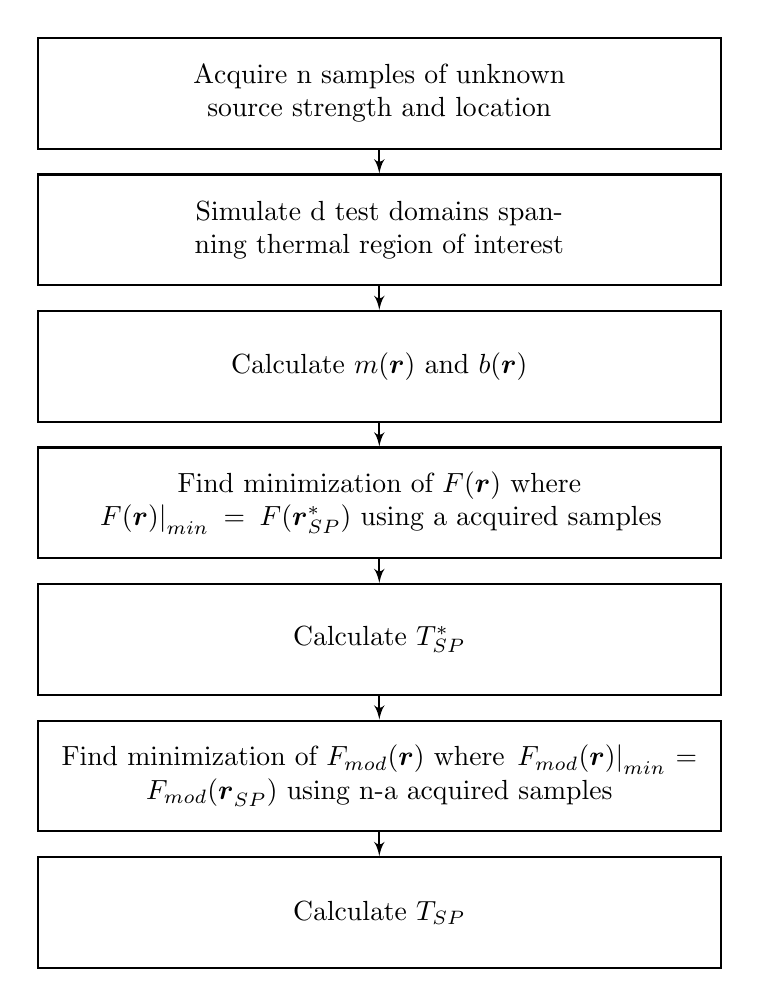
\begin{tikzpicture}[auto,
    %decision/.style={diamond, draw=black, thick, fill=white,
    %text width=8em, text badly centered,
    %inner sep=1pt, font=\sffamily\small},
    block_center/.style ={rectangle, draw=black, thick, fill=white,
      text width=24em, text centered,
      minimum height=4em},
    block_left/.style ={rectangle, draw=black, thick, fill=white,
      text width=16em, text ragged, minimum height=4em, inner sep=6pt},
    block_noborder/.style ={rectangle, draw=none, thick, fill=none,
      text width=18em, text centered, minimum height=1em},
    block_assign/.style ={rectangle, draw=black, thick, fill=white,
      text width=18em, text ragged, minimum height=3em, inner sep=6pt},
    block_lost/.style ={rectangle, draw=black, thick, fill=white,
      text width=16em, text ragged, minimum height=3em, inner sep=6pt},
      line/.style ={draw, thick, -latex', shorten >=0pt}]
    % outlining the flowchart using the PGF/TikZ matrix funtion
    \matrix [column sep=5mm,row sep=3mm] {
			\node [block_center] (acquire) {Acquire n samples of unknown source strength and location};\\
		  \node [block_center] (sim) {Simulate d test domains spanning thermal region of interest};	\\		
			\node [block_center] (calcm) {Calculate $m( \bv r)$ and $b( \bv r)$};	\\		
			\node [block_center] (minf) {Find minimization of $F( \bv r)$ where $\left. F( \bv r) \right|_{min} = F(\bv{r^{\ast}_{SP}})$ using a acquired samples};	\\					
			\node [block_center] (calcts) {Calculate $T^{\ast}_{SP}$};	\\		
			\node [block_center] (minfmod) {Find minimization of $F_{mod}(\bv r)$ where $\left. F_{mod}( \bv r) \right|_{min} = F_{mod}(\bv{r^{ }_{SP}})$ using n-a acquired samples};	\\					
			\node [block_center] (calct) {Calculate $T_{SP}$};	\\					
   };% end matrix
    % connecting nodes with paths
    \begin{scope}[every path/.style=line]
      \path (acquire)     -- (sim);
			\path (sim)     -- (calcm);
			\path (calcm)     -- (minf);
			\path (minf)     -- (calcts);
			\path (calcts)     -- (minfmod);
			\path (minfmod)     -- (calct);			
    \end{scope}		
  \end{tikzpicture}
\caption{Flow chart of the predictor - corrector methodology \cite{ijhmt1} }
\label{fig:flowchart}
\end{figure}




\section{Methodology}
  
The optimization of the predictor - corrector method begins with identifying the function needing to be optimized.  The function desired needs to minimize the error associated with the prediction of the source temperature, since the predictor step defines the effectiveness of the corrector step.  Thus, we start with \cref{eq:Tsp} and determine the error of this function.  \Cref{eq:Tsp} is rewritten here with a few modifications.  The first aspect to identify is the change from $ \bv{r^{\ast}_{SP}}$ to $\bv{r_0}$, indicating that $\bv{r_0}$ is fixed prior to the optimization.  The $\bv{\Delta}$ is now included in the local temperature function to keep the relative distance during the optimization process.  Lastly is the addition of $\bv{\delta}$,  that is used to calculate the error for the entire domain by varying the location of the sampled points.
%
\begin{equation}
\centering
T_{SO} = \frac{1}{n} \{ \sum^{n}_{i=0} [ m\left(\bv{r_0} + \bv{\Delta_i} + \bv{\delta} \right) T\left(\bv{r_0} + \bv{\Delta_i}\right)  + b\left(\bv{r_0} + \bv{\Delta_i} + \bv{\delta}\right) ] \}
\label{eq:Tsp2}
\end{equation}
%
The error of \cref{eq:Tsp2} is written via \cref{eq:optfunct1} where $\varepsilon$ is the percent error.
%
\begin{equation}
\centering
\left| \frac{T_{SO} - T_S}{T_S-T_{\infty}}\right| \times 100 = \varepsilon 
\label{eq:optfunct1}
\end{equation}
%
The effectiveness of any one sampled data point is determined by how much it reduces the error at the test location and how much it increases the error everywhere else.  This is accomplished with the area defined by \cref{eq:optfunct1} at a specified error $\varepsilon$.

The method used minimizes the area enclosed by \cref{eq:optfunct1} at a defined $\varepsilon$ using one variable sample point.  That is to say that the initial point is selected as $\bv{r_0}$, which through the optimization yields, $\bv{r_1}$.  Repeating this process, using $\bv{r_0}$ and $\bv{r_1}$, the optimization process can find $\bv{r_2}$.  If more accurate results are desired, this process may be continued indefinitely.  For this particular inverse problem of the plume in a crosswind, three total sampling points were enough to achieve the desired accuracy, i.e. better than the experimental temperature error of $2\%$.  This process is repeated for many iterations varying $U_\infty$, $T_S$, and $\bv{r_0}$ to cover the domain.  

While any global optimization method would likely work the genetic algorithm was chosen due to its robustness and ease of use.  A canned genetic algorithm within the Mathworks Matlab\cite{matlabsoftware} optimization toolkit was utilized.  The genetic algorithm is a bio-mimetic optimization strategy specifically designed to be robust and solve for global minimums \cite{onwubiko}.  The genetic algorithm roughly mimics the evolution of a species with the design parameters called chromosomes.  The process starts by generating a large pool of chromosomes, each is checked against function needing to be optimized and ranked.  A selection process then chooses pairs of parents to generate the next generation.  Information from each of the chromosomes is used to make children chromosomes in what is known as crossover.  These new chromosomes have a small chance at mutation, which randomly changes a design parameter.  This reduces the chances of stagnation of the chromosome pool.  This process repeats until a stopping criteria is met, usually the total number of iterations or a count of iterations where the best performing chromosome does not change.  In the case of the Matlab version those default numbers are 100 and 50 respectively.

The only parameters changed from the Matlab defaults are listed in \cref{tab:gaparam}.  Due to the repetitive nature and large total iteration count of the methodology, the population size of the genetic algorithm was kept small to reduce computation time.  While this could reduce the effectiveness of the genetic algorithm the large sample size reduces the effects.  Several test cases were performed with much larger populations and generation counts and found that the resultant solution was very similar to the reduced population version.  The computation time was approximately 2 weeks and run on a twin processor, twelve core computer at 3.2GHz with 32GB of RAM.
A flow chart of the methodology is shown in \cref{fig:optflowchart}.
%
\begin{table}[!h!t!b!p]
\begin{center}
\begin{tabular}{ l c}
\hline
Parameter & Value \\ \hline
PopulationSize & 60 \\
Generations & 200 \\ \hline
 \end{tabular}
 \end{center}
\caption{Genetic algorithm parameters}
\label{tab:gaparam}
\end{table}
%
%
\begin{figure}[!tbp]
\centering
  % setting the typeface to sans serif and the font size to small
  % the scope local to the environment
  \sffamily
  \footnotesize
  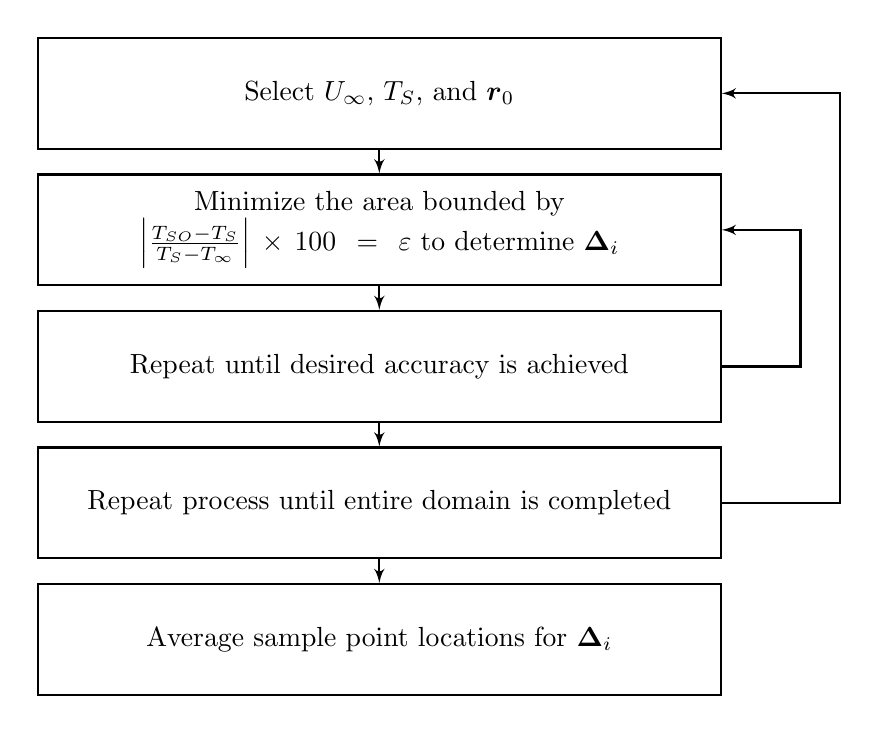
\begin{tikzpicture}[auto,
    %decision/.style={diamond, draw=black, thick, fill=white,
    %text width=8em, text badly centered,
    %inner sep=1pt, font=\sffamily\small},
    block_center/.style ={rectangle, draw=black, thick, fill=white,
      text width=24em, text centered,
      minimum height=4em},
    block_left/.style ={rectangle, draw=black, thick, fill=white,
      text width=16em, text ragged, minimum height=4em, inner sep=6pt},
    block_noborder/.style ={rectangle, draw=none, thick, fill=none,
      text width=18em, text centered, minimum height=1em},
    block_assign/.style ={rectangle, draw=black, thick, fill=white,
      text width=18em, text ragged, minimum height=3em, inner sep=6pt},
    block_lost/.style ={rectangle, draw=black, thick, fill=white,
      text width=16em, text ragged, minimum height=3em, inner sep=6pt},
      line/.style ={draw, thick, -latex', shorten >=0pt}]
    % outlining the flowchart using the PGF/TikZ matrix funtion
    \matrix [column sep=5mm,row sep=3mm] {
			\node [block_center] (select) {Select $U_\infty$, $T_S$, and $\bv{r_0}$};\\
		  \node [block_center] (mini) {Minimize the area bounded by $\left| \frac{T_{SO} - T_S}{T_S-T_{\infty}} \right| \times 100 = \varepsilon$ to determine $\bv{\Delta_i}$};	\\		
			\node [block_center] (repeat) {Repeat until desired accuracy is achieved};	\\		
			\node [block_center] (ra) {Repeat process until entire domain is completed};	\\		
			\node [block_center] (end) {Average sample point locations for $\bv{\Delta_i}$};	\\		
   };% end matrix
    % connecting nodes with paths
    \begin{scope}[every path/.style=line]
      \path (select)     -- (mini);
			\path (mini)     -- (repeat);
			\path (repeat)     -- (ra);
			\path (repeat.east)   |- ++(1,0) |- (mini.east);
			\path (ra.east) |- ++(1.5,0) |- (select.east);
			\path (ra) -- (end);
    \end{scope}		
    
    
  \end{tikzpicture}
\caption{Flow chart of the presented methodology}
\label{fig:optflowchart}
\end{figure}


\section{Results and discussions}

The methodology requires a large sampling of the domain of interest to function properly.  The selected parameters are varied as shown in \cref{tab:optparam}.  These parameters were selected to thoroughly cover the experimental domain, which has physical limitations.  The material properties of the wind tunnel limit $T_S$ to $450\, K$.  Which in turn limits $U_{\infty}$ to approximately $1.0, m/s$ due to the plume being pushed too close to the lower boundary and becoming difficult to measure accurately.  The parameter $r_{axial}$ is the coordinate in the direction of the free stream, and $r_{perp}$ is the coordinate perpendicular to the free stream.  The ranges for both $r_{axial}$ and $r_{perp}$ were selected to completely cover the effective range of the plume.  The end result of using these selected parameters is 1050 total samples in the domain.
\begin{table}[!h!t!b!p]
\begin{center}
\begin{tabular}{ r c c c }
\hline
 Parameter & Minimum & Maximum & Increments \\ \hline 
$U_\infty \, (m/s)$ & 0.0 & 1.0 & 0.2 \\
$T_S \, (K)$ & 350 & 450 & 25 \\
$r_{axial}$ $(mm)$ & 0 & 150 & 25 \\
$r_{perp}$ $(mm)$ & 0 & 10 & 2.5 \\ \hline
 \end{tabular}
\caption{Variable domain parameters used for optimization}
\label{tab:optparam}
\end{center}
\end{table}

The results of this optimization is a ``perfect'' search shape for each of the aforementioned domain parameters.  However, the point of the inverse problem is such that the domain parameter is not known and determining the domain parameters are in fact the desired result of the inverse methodology.  Therefore to make the optimization worthwhile all of the $\bv{r_1}$'s are averaged together and similarly for $\bv{r_2}$.

The result from averaging the 1050 domain optimization is shown in \cref{tab:optresults}.  While the methodology is capable of providing more sample points, the accuracy provided by the three sample points was more than enough to accurately solve the described inverse problem.  The predictor step uses the first and second samples, while the corrector step uses the first and third samples.  That is to say $\bv{r_0}$ is reused as previously described.
\begin{table}[!h!t!b!p]
\begin{center}
\begin{tabular}{ c c }
\hline
 Sample Point & $\bv{\Delta} \, (mm)$  \\ \hline 
0 & (0.0, 0.0) \\
1 & (1.7, 3.5) \\
2 & (2.8, 0.6) \\  \hline
 \end{tabular}
\caption{Search shape results of averaging over the domain}
\label{tab:optresults}
\end{center}
\end{table}

For comparisons sake, \cref{tab:original} contains the original search shape used in the inverse solution.  This search shape was selected based upon intuition only.  The original samples one through three were used for the predictor stage and one, four, and five were used in the corrector stage.
%
\begin{table}[!h!t!b!p]
\begin{center}
\begin{tabular}{ c c }
\hline
 Sample Point & $\bv{\Delta} \, (mm)$  \\ \hline 
1 & (0.0, 0.0) \\
2 & (1.0, 0.0) \\
3 & (2.0, 0.0) \\
4 & (0.0, 1.0) \\
5 & (0.0, 2.0) \\ \hline
 \end{tabular}
\caption{Original search shape for this inverse solution}
\label{tab:original}
\end{center}
\end{table}

The error plots of \cref{fig:ERO1PT,fig:ERO2PT,fig:ERO3PT,fig:ERN2PT,fig:ERN3PT} demonstrate the effectiveness of the new sampling points.  These plots are explained as the predicted source temperature error if an incorrect location was predicted.  The correct result location is at $\bv{r_0} = (100.0,\,2.0)\,mm$ and is indicated by an `x'.  The shaded regions indicate how much error is associated with the prediction stage as it searches for a match within the domain.  That is to say it is a plot of $\varepsilon$ from \cref{eq:optfunct1}.  The $x$ and $y$ distances are normalized to the heater width of $25.4\,mm$.  The size and scale of each plot is kept the same for comparison's sake.  The largest contour region is empty space and indicates an error of $20\%$ or more.

\Cref{fig:ERO1PT} is an error plot for 1 sample point.  This is the same for both the original sampled data and the optimized sampled data.  The darkest shaded regions indicate a $5\%$ or less error in source temperature for those locations, indicating that any of those regions are viable answers.  The biggest issue is that there are many local minimums, which will never converge to the correct solution.  \Cref{fig:ERN2PT,fig:ERO2PT} and \cref{fig:ERN3PT,fig:ERO3PT} show the differences between the original sampled data pattern and the optimized sampled data pattern.  In both cases the error from the optimized sampled data is smaller and more confined than the original sampled data.  
%
\begin{figure}[!htbp]
	\centering
	\setlength\figureheight{4cm} 
	\setlength\figurewidth{4cm}
	% This file was created by matlab2tikz v0.4.0.
% Copyright (c) 2008--2013, Nico Schlömer <nico.schloemer@gmail.com>
% All rights reserved.
% 
% The latest updates can be retrieved from
%   http://www.mathworks.com/matlabcentral/fileexchange/22022-matlab2tikz
% where you can also make suggestions and rate matlab2tikz.
% 
% 
% 

% defining custom colors
\definecolor{mycolor1}{rgb}{0.253968253968254,0.253968253968254,0.253968253968254}%
\definecolor{mycolor2}{rgb}{0.507936507936508,0.507936507936508,0.507936507936508}%
\definecolor{mycolor3}{rgb}{0.761904761904762,0.761904761904762,0.761904761904762}%

\begin{tikzpicture}

\begin{axis}[%
width=\figurewidth,
height=\figureheight,
scale only axis,
xmin=0,
xmax=7,
xlabel={Normalized Axial Distance},
ymin=0,
ymax=0.5,
ylabel={Normalized Distance Above Surface},
axis x line*=bottom,
axis y line*=left,
colormap/blackwhite,
colorbar horizontal,
point meta min=0,
point meta max=20
]

\addplot [solid,fill=black,draw=black,forget plot] table[row sep=crcr]{
-0.393700787401575 0.600001987202854\\
-0.346240157480315 0.600001987202854\\
-0.298779527559055 0.600001987202854\\
-0.251318897637795 0.600001987202854\\
-0.203858267716535 0.600001987202854\\
-0.156397637795276 0.600001987202854\\
-0.108937007874016 0.600001987202854\\
-0.0614763779527559 0.600001987202854\\
-0.0140157480314961 0.600001987202854\\
0.0334448818897638 0.600001987202854\\
0.0809055118110236 0.600001987202854\\
0.128366141732283 0.600001987202854\\
0.175826771653543 0.600001987202854\\
0.223287401574803 0.600001987202854\\
0.270748031496063 0.600001987202854\\
0.318208661417323 0.600001987202854\\
0.365669291338583 0.600001987202854\\
0.413129921259843 0.600001987202854\\
0.460590551181102 0.600001987202854\\
0.508051181102362 0.600001987202854\\
0.555511811023622 0.600001987202854\\
0.602972440944882 0.600001987202854\\
0.650433070866142 0.600001987202854\\
0.697893700787402 0.600001987202854\\
0.745354330708662 0.600001987202854\\
0.792814960629921 0.600001987202854\\
0.840275590551181 0.600001987202854\\
0.887736220472441 0.600001987202854\\
0.935196850393701 0.600001987202854\\
0.98265748031496 0.600001987202854\\
1.03011811023622 0.600001987202854\\
1.07757874015748 0.600001987202854\\
1.12503937007874 0.600001987202854\\
1.1725 0.600001987202854\\
1.21996062992126 0.600001987202854\\
1.26742125984252 0.600001987202854\\
1.31488188976378 0.600001987202854\\
1.36234251968504 0.600001987202854\\
1.4098031496063 0.600001987202854\\
1.45726377952756 0.600001987202854\\
1.50472440944882 0.600001987202854\\
1.55218503937008 0.600001987202854\\
1.59964566929134 0.600001987202854\\
1.6471062992126 0.600001987202854\\
1.69456692913386 0.600001987202854\\
1.74202755905512 0.600001987202854\\
1.78948818897638 0.600001987202854\\
1.83694881889764 0.600001987202854\\
1.8844094488189 0.600001987202854\\
1.93187007874016 0.600001987202854\\
1.97933070866142 0.600001987202854\\
2.02679133858268 0.600001987202854\\
2.07425196850394 0.600001987202854\\
2.1217125984252 0.600001987202854\\
2.16917322834646 0.600001987202854\\
2.21663385826772 0.600001987202854\\
2.26409448818898 0.600001987202854\\
2.31155511811024 0.600001987202854\\
2.3590157480315 0.600001987202854\\
2.40647637795276 0.600001987202854\\
2.45393700787402 0.600001987202854\\
2.50139763779528 0.600001987202854\\
2.54885826771654 0.600001987202854\\
2.5963188976378 0.600001987202854\\
2.64377952755906 0.600001987202854\\
2.69124015748032 0.600001987202854\\
2.73870078740157 0.600001987202854\\
2.78616141732283 0.600001987202854\\
2.83362204724409 0.600001987202854\\
2.88108267716535 0.600001987202854\\
2.92854330708661 0.600001987202854\\
2.97600393700787 0.600001987202854\\
3.02346456692913 0.600001987202854\\
3.07092519685039 0.600001987202854\\
3.11838582677165 0.600001987202854\\
3.16584645669291 0.600001987202854\\
3.21330708661417 0.600001987202854\\
3.26076771653543 0.600001987202854\\
3.30822834645669 0.600001987202854\\
3.35568897637795 0.600001987202854\\
3.40314960629921 0.600001987202854\\
3.45061023622047 0.600001987202854\\
3.49807086614173 0.600001987202854\\
3.54553149606299 0.600001987202854\\
3.59299212598425 0.600001987202854\\
3.64045275590551 0.600001987202854\\
3.68791338582677 0.600001987202854\\
3.73537401574803 0.600001987202854\\
3.78283464566929 0.600001987202854\\
3.83029527559055 0.600001987202854\\
3.87775590551181 0.600001987202854\\
3.92521653543307 0.600001987202854\\
3.97267716535433 0.600001987202854\\
4.02013779527559 0.600001987202854\\
4.06759842519685 0.600001987202854\\
4.11505905511811 0.600001987202854\\
4.16251968503937 0.600001987202854\\
4.20998031496063 0.600001987202854\\
4.25744094488189 0.600001987202854\\
4.30490157480315 0.600001987202854\\
4.35236220472441 0.600001987202854\\
4.39982283464567 0.600001987202854\\
4.44728346456693 0.600001987202854\\
4.49474409448819 0.600001987202854\\
4.54220472440945 0.600001987202854\\
4.58966535433071 0.600001987202854\\
4.63712598425197 0.600001987202854\\
4.68458661417323 0.600001987202854\\
4.73204724409449 0.600001987202854\\
4.77950787401575 0.600001987202854\\
4.82696850393701 0.600001987202854\\
4.87442913385827 0.600001987202854\\
4.92188976377953 0.600001987202854\\
4.96935039370079 0.600001987202854\\
5.01681102362205 0.600001987202854\\
5.06427165354331 0.600001987202854\\
5.11173228346457 0.600001987202854\\
5.15919291338583 0.600001987202854\\
5.20665354330709 0.600001987202854\\
5.25411417322835 0.600001987202854\\
5.30157480314961 0.600001987202854\\
5.34903543307087 0.600001987202854\\
5.39649606299213 0.600001987202854\\
5.44395669291338 0.600001987202854\\
5.49141732283465 0.600001987202854\\
5.53887795275591 0.600001987202854\\
5.58633858267717 0.600001987202854\\
5.63379921259842 0.600001987202854\\
5.68125984251968 0.600001987202854\\
5.72872047244094 0.600001987202854\\
5.7761811023622 0.600001987202854\\
5.82364173228346 0.600001987202854\\
5.87110236220472 0.600001987202854\\
5.91856299212598 0.600001987202854\\
5.96602362204724 0.600001987202854\\
6.0134842519685 0.600001987202854\\
6.06094488188976 0.600001987202854\\
6.10840551181102 0.600001987202854\\
6.15586614173228 0.600001987202854\\
6.20332677165354 0.600001987202854\\
6.2507874015748 0.600001987202854\\
6.29824803149606 0.600001987202854\\
6.34570866141732 0.600001987202854\\
6.39316929133858 0.600001987202854\\
6.44062992125984 0.600001987202854\\
6.4880905511811 0.600001987202854\\
6.53555118110236 0.600001987202854\\
6.58301181102362 0.600001987202854\\
6.63047244094488 0.600001987202854\\
6.67793307086614 0.600001987202854\\
6.7253937007874 0.600001987202854\\
6.77285433070866 0.600001987202854\\
6.82031496062992 0.600001987202854\\
6.86777559055118 0.600001987202854\\
6.91523622047244 0.600001987202854\\
6.9626968503937 0.600001987202854\\
7.01015748031496 0.600001987202854\\
7.05761811023622 0.600001987202854\\
7.10507874015748 0.600001987202854\\
7.15253937007874 0.600001987202854\\
7.2 0.600001987202854\\
7.20000474558843 0.6\\
7.20000474558843 0.580125984251968\\
7.20000474558843 0.560251968503937\\
7.20000474558843 0.540377952755905\\
7.20000474558843 0.520503937007874\\
7.20000474558843 0.500629921259843\\
7.20000474558843 0.480755905511811\\
7.20000474558843 0.460881889763779\\
7.20000474558843 0.441007874015748\\
7.20000474558843 0.421133858267717\\
7.20000474558843 0.401259842519685\\
7.20000474558843 0.381385826771654\\
7.20000474558843 0.361511811023622\\
7.20000474558843 0.341637795275591\\
7.20000474558843 0.321763779527559\\
7.20000474558843 0.301889763779528\\
7.20000474558843 0.282015748031496\\
7.20000474558843 0.262141732283465\\
7.2000044909465 0.242267716535433\\
7.20000409657343 0.222393700787401\\
7.20000378126375 0.20251968503937\\
7.20000353233019 0.182645669291338\\
7.20000333133117 0.162771653543307\\
7.20000318093718 0.142897637795276\\
7.20000308815432 0.123023622047244\\
7.20000302494975 0.103149606299213\\
7.20000298659693 0.0832755905511811\\
7.20000296932143 0.0634015748031495\\
7.20000296257056 0.0435275590551181\\
7.20000295904314 0.0236535433070866\\
7.20000295803653 0.00377952755905507\\
7.20000474558843 -0.0160944881889764\\
7.20000474558843 -0.0359685039370079\\
7.20000474558843 -0.0558425196850394\\
7.20000474558843 -0.0757165354330709\\
7.20000474558843 -0.0955905511811024\\
7.20000474558843 -0.115464566929134\\
7.20000474558843 -0.135338582677165\\
7.20000474558843 -0.155212598425197\\
7.20000474558843 -0.175086614173228\\
7.20000474558843 -0.19496062992126\\
7.20000474558843 -0.214834645669291\\
7.20000474558843 -0.234708661417323\\
7.20000474558843 -0.254582677165354\\
7.20000474558843 -0.274456692913386\\
7.20000474558843 -0.294330708661417\\
7.20000474558843 -0.314204724409449\\
7.20000474558843 -0.33407874015748\\
7.20000474558843 -0.353952755905512\\
7.20000474558843 -0.373826771653543\\
7.20000474558843 -0.393700787401575\\
7.2 -0.393702774604429\\
7.15253937007874 -0.393702774604429\\
7.10507874015748 -0.393702774604429\\
7.05761811023622 -0.393702774604429\\
7.01015748031496 -0.393702774604429\\
6.9626968503937 -0.393702774604429\\
6.91523622047244 -0.393702774604429\\
6.86777559055118 -0.393702774604429\\
6.82031496062992 -0.393702774604429\\
6.77285433070866 -0.393702774604429\\
6.7253937007874 -0.393702774604429\\
6.67793307086614 -0.393702774604429\\
6.63047244094488 -0.393702774604429\\
6.58301181102362 -0.393702774604429\\
6.53555118110236 -0.393702774604429\\
6.4880905511811 -0.393702774604429\\
6.44062992125984 -0.393702774604429\\
6.39316929133858 -0.393702774604429\\
6.34570866141732 -0.393702774604429\\
6.29824803149606 -0.393702774604429\\
6.2507874015748 -0.393702774604429\\
6.20332677165354 -0.393702774604429\\
6.15586614173228 -0.393702774604429\\
6.10840551181102 -0.393702774604429\\
6.06094488188976 -0.393702774604429\\
6.0134842519685 -0.393702774604429\\
5.96602362204724 -0.393702774604429\\
5.91856299212598 -0.393702774604429\\
5.87110236220472 -0.393702774604429\\
5.82364173228346 -0.393702774604429\\
5.7761811023622 -0.393702774604429\\
5.72872047244094 -0.393702774604429\\
5.68125984251968 -0.393702774604429\\
5.63379921259842 -0.393702774604429\\
5.58633858267717 -0.393702774604429\\
5.53887795275591 -0.393702774604429\\
5.49141732283465 -0.393702774604429\\
5.44395669291338 -0.393702774604429\\
5.39649606299213 -0.393702774604429\\
5.34903543307087 -0.393702774604429\\
5.30157480314961 -0.393702774604429\\
5.25411417322835 -0.393702774604429\\
5.20665354330709 -0.393702774604429\\
5.15919291338583 -0.393702774604429\\
5.11173228346457 -0.393702774604429\\
5.06427165354331 -0.393702774604429\\
5.01681102362205 -0.393702774604429\\
4.96935039370079 -0.393702774604429\\
4.92188976377953 -0.393702774604429\\
4.87442913385827 -0.393702774604429\\
4.82696850393701 -0.393702774604429\\
4.77950787401575 -0.393702774604429\\
4.73204724409449 -0.393702774604429\\
4.68458661417323 -0.393702774604429\\
4.63712598425197 -0.393702774604429\\
4.58966535433071 -0.393702774604429\\
4.54220472440945 -0.393702774604429\\
4.49474409448819 -0.393702774604429\\
4.44728346456693 -0.393702774604429\\
4.39982283464567 -0.393702774604429\\
4.35236220472441 -0.393702774604429\\
4.30490157480315 -0.393702774604429\\
4.25744094488189 -0.393702774604429\\
4.20998031496063 -0.393702774604429\\
4.16251968503937 -0.393702774604429\\
4.11505905511811 -0.393702774604429\\
4.06759842519685 -0.393702774604429\\
4.02013779527559 -0.393702774604429\\
3.97267716535433 -0.393702774604429\\
3.92521653543307 -0.393702774604429\\
3.87775590551181 -0.393702774604429\\
3.83029527559055 -0.393702774604429\\
3.78283464566929 -0.393702774604429\\
3.73537401574803 -0.393702774604429\\
3.68791338582677 -0.393702774604429\\
3.64045275590551 -0.393702774604429\\
3.59299212598425 -0.393702774604429\\
3.54553149606299 -0.393702774604429\\
3.49807086614173 -0.393702774604429\\
3.45061023622047 -0.393702774604429\\
3.40314960629921 -0.393702774604429\\
3.35568897637795 -0.393702774604429\\
3.30822834645669 -0.393702774604429\\
3.26076771653543 -0.393702774604429\\
3.21330708661417 -0.393702774604429\\
3.16584645669291 -0.393702774604429\\
3.11838582677165 -0.393702774604429\\
3.07092519685039 -0.393702774604429\\
3.02346456692913 -0.393702774604429\\
2.97600393700787 -0.393702774604429\\
2.92854330708661 -0.393702774604429\\
2.88108267716535 -0.393702774604429\\
2.83362204724409 -0.393702774604429\\
2.78616141732283 -0.393702774604429\\
2.73870078740157 -0.393702774604429\\
2.69124015748032 -0.393702774604429\\
2.64377952755906 -0.393702774604429\\
2.5963188976378 -0.393702774604429\\
2.54885826771654 -0.393702774604429\\
2.50139763779528 -0.393702774604429\\
2.45393700787402 -0.393702774604429\\
2.40647637795276 -0.393702774604429\\
2.3590157480315 -0.393702774604429\\
2.31155511811024 -0.393702774604429\\
2.26409448818898 -0.393702774604429\\
2.21663385826772 -0.393702774604429\\
2.16917322834646 -0.393702774604429\\
2.1217125984252 -0.393702774604429\\
2.07425196850394 -0.393702774604429\\
2.02679133858268 -0.393702774604429\\
1.97933070866142 -0.393702774604429\\
1.93187007874016 -0.393702774604429\\
1.8844094488189 -0.393702774604429\\
1.83694881889764 -0.393702774604429\\
1.78948818897638 -0.393702774604429\\
1.74202755905512 -0.393702774604429\\
1.69456692913386 -0.393702774604429\\
1.6471062992126 -0.393702774604429\\
1.59964566929134 -0.393702774604429\\
1.55218503937008 -0.393702774604429\\
1.50472440944882 -0.393702774604429\\
1.45726377952756 -0.393702774604429\\
1.4098031496063 -0.393702774604429\\
1.36234251968504 -0.393702774604429\\
1.31488188976378 -0.393702774604429\\
1.26742125984252 -0.393702774604429\\
1.21996062992126 -0.393702774604429\\
1.1725 -0.393702774604429\\
1.12503937007874 -0.393702774604429\\
1.07757874015748 -0.393702774604429\\
1.03011811023622 -0.393702774604429\\
0.98265748031496 -0.393702774604429\\
0.935196850393701 -0.393702774604429\\
0.887736220472441 -0.393702774604429\\
0.840275590551181 -0.393702774604429\\
0.792814960629921 -0.393702774604429\\
0.745354330708662 -0.393702774604429\\
0.697893700787402 -0.393702774604429\\
0.650433070866142 -0.393702774604429\\
0.602972440944882 -0.393702774604429\\
0.555511811023622 -0.393702774604429\\
0.508051181102362 -0.393702774604429\\
0.460590551181102 -0.393702774604429\\
0.413129921259843 -0.393702774604429\\
0.365669291338583 -0.393702774604429\\
0.318208661417323 -0.393702774604429\\
0.270748031496063 -0.393702774604429\\
0.223287401574803 -0.393702774604429\\
0.175826771653543 -0.393702774604429\\
0.128366141732283 -0.393702774604429\\
0.0809055118110236 -0.393702774604429\\
0.0334448818897638 -0.393702774604429\\
-0.0140157480314961 -0.393702774604429\\
-0.0614763779527559 -0.393702774604429\\
-0.108937007874016 -0.393702774604429\\
-0.156397637795276 -0.393702774604429\\
-0.203858267716535 -0.393702774604429\\
-0.251318897637795 -0.393702774604429\\
-0.298779527559055 -0.393702774604429\\
-0.346240157480315 -0.393702774604429\\
-0.393700787401575 -0.393702774604429\\
-0.393705532990008 -0.393700787401575\\
-0.393705532990008 -0.373826771653543\\
-0.393705532990008 -0.353952755905512\\
-0.393705532990008 -0.33407874015748\\
-0.393705532990008 -0.314204724409449\\
-0.393705532990008 -0.294330708661417\\
-0.393705532990008 -0.274456692913386\\
-0.393705532990008 -0.254582677165354\\
-0.393705532990008 -0.234708661417323\\
-0.393705532990008 -0.214834645669291\\
-0.393705532990008 -0.19496062992126\\
-0.393705532990008 -0.175086614173228\\
-0.393705532990008 -0.155212598425197\\
-0.393705532990008 -0.135338582677165\\
-0.393705532990008 -0.115464566929134\\
-0.393705532990008 -0.0955905511811024\\
-0.393705532990008 -0.0757165354330709\\
-0.393705532990008 -0.0558425196850394\\
-0.393705532990008 -0.0359685039370079\\
-0.393705532990008 -0.0160944881889764\\
-0.393705532990008 0.00377952755905507\\
-0.393705532990008 0.0236535433070866\\
-0.393705532990008 0.0435275590551181\\
-0.393705532990008 0.0634015748031495\\
-0.393705532990008 0.0832755905511811\\
-0.393705532990008 0.103149606299213\\
-0.393705532990008 0.123023622047244\\
-0.393705532990008 0.142897637795276\\
-0.393705532990008 0.162771653543307\\
-0.393705532990008 0.182645669291338\\
-0.393705532990008 0.20251968503937\\
-0.393705532990008 0.222393700787401\\
-0.393705532990008 0.242267716535433\\
-0.393705532990008 0.262141732283465\\
-0.393705532990008 0.282015748031496\\
-0.393705532990008 0.301889763779528\\
-0.393705532990008 0.321763779527559\\
-0.393705532990008 0.341637795275591\\
-0.393705532990008 0.361511811023622\\
-0.393705532990008 0.381385826771654\\
-0.393705532990008 0.401259842519685\\
-0.393705532990008 0.421133858267717\\
-0.393705532990008 0.441007874015748\\
-0.393705532990008 0.460881889763779\\
-0.393705532990008 0.480755905511811\\
-0.393705532990008 0.500629921259843\\
-0.393705532990008 0.520503937007874\\
-0.393705532990008 0.540377952755905\\
-0.393705532990008 0.560251968503937\\
-0.393705532990008 0.580125984251968\\
-0.393705532990008 0.6\\
-0.393700787401575 0.600001987202854\\
};

\addplot [solid,fill=mycolor1,draw=black,forget plot] table[row sep=crcr]{
-0.393700787401575 0.600001860937636\\
-0.346240157480315 0.600001860937636\\
-0.298779527559055 0.600001860937636\\
-0.251318897637795 0.600001860937636\\
-0.203858267716535 0.600001860937636\\
-0.156397637795276 0.600001860937636\\
-0.108937007874016 0.600001860937636\\
-0.0614763779527559 0.600001860937636\\
-0.0140157480314961 0.600001860937636\\
0.0334448818897638 0.600001860937636\\
0.0809055118110236 0.600001860937636\\
0.128366141732283 0.600001860937636\\
0.175826771653543 0.600001860937636\\
0.223287401574803 0.600001860937636\\
0.270748031496063 0.600001860937636\\
0.318208661417323 0.600001860937636\\
0.365669291338583 0.600001860937636\\
0.413129921259843 0.600001860937636\\
0.460590551181102 0.600001860937636\\
0.508051181102362 0.600001860937636\\
0.555511811023622 0.600001860937636\\
0.602972440944882 0.600001860937636\\
0.650433070866142 0.600001860937636\\
0.697893700787402 0.600001860937636\\
0.745354330708662 0.600001860937636\\
0.792814960629921 0.600001860937636\\
0.840275590551181 0.600001860937636\\
0.887736220472441 0.600001860937636\\
0.935196850393701 0.600001860937636\\
0.98265748031496 0.600001860937636\\
1.03011811023622 0.600001860937636\\
1.07757874015748 0.600001860937636\\
1.12503937007874 0.600001860937636\\
1.1725 0.600001860937636\\
1.21996062992126 0.600001860937636\\
1.26742125984252 0.600001860937636\\
1.31488188976378 0.600001860937636\\
1.36234251968504 0.600001860937636\\
1.4098031496063 0.600001860937636\\
1.45726377952756 0.600001860937636\\
1.50472440944882 0.600001860937636\\
1.55218503937008 0.600001860937636\\
1.59964566929134 0.600001860937636\\
1.6471062992126 0.600001860937636\\
1.69456692913386 0.600001860937636\\
1.74202755905512 0.600001860937636\\
1.78948818897638 0.600001860937636\\
1.83694881889764 0.600001860937636\\
1.8844094488189 0.600001860937636\\
1.93187007874016 0.600001860937636\\
1.97933070866142 0.600001860937636\\
2.02679133858268 0.600001860937636\\
2.07425196850394 0.600001860937636\\
2.1217125984252 0.600001860937636\\
2.16917322834646 0.600001860937636\\
2.21663385826772 0.600001860937636\\
2.26409448818898 0.600001860937636\\
2.31155511811024 0.600001860937636\\
2.3590157480315 0.600001860937636\\
2.40647637795276 0.600001860937636\\
2.45393700787402 0.600001860937636\\
2.50139763779528 0.600001860937636\\
2.54885826771654 0.600001860937636\\
2.5963188976378 0.600001860937636\\
2.64377952755906 0.600001860937636\\
2.69124015748032 0.600001860937636\\
2.73870078740157 0.600001860937636\\
2.78616141732283 0.600001860937636\\
2.83362204724409 0.600001860937636\\
2.88108267716535 0.600001860937636\\
2.92854330708661 0.600001860937636\\
2.97600393700787 0.600001860937636\\
3.02346456692913 0.600001860937636\\
3.07092519685039 0.600001860937636\\
3.11838582677165 0.600001860937636\\
3.16584645669291 0.600001860937636\\
3.21330708661417 0.600001860937636\\
3.26076771653543 0.600001860937636\\
3.30822834645669 0.600001860937636\\
3.35568897637795 0.600001860937636\\
3.40314960629921 0.600001860937636\\
3.45061023622047 0.600001860937636\\
3.49807086614173 0.600001860937636\\
3.54553149606299 0.600001860937636\\
3.59299212598425 0.600001860937636\\
3.64045275590551 0.600001860937636\\
3.68791338582677 0.600001860937636\\
3.73537401574803 0.600001860937636\\
3.78283464566929 0.600001860937636\\
3.83029527559055 0.600001860937636\\
3.87775590551181 0.600001860937636\\
3.92521653543307 0.600001860937636\\
3.97267716535433 0.600001860937636\\
4.02013779527559 0.600001860937636\\
4.06759842519685 0.600001860937636\\
4.11505905511811 0.600001860937636\\
4.16251968503937 0.600001860937636\\
4.20998031496063 0.600001860937636\\
4.25744094488189 0.600001860937636\\
4.30490157480315 0.600001860937636\\
4.35236220472441 0.600001860937636\\
4.39982283464567 0.600001860937636\\
4.44728346456693 0.600001860937636\\
4.49474409448819 0.600001860937636\\
4.54220472440945 0.600001860937636\\
4.58966535433071 0.600001860937636\\
4.63712598425197 0.600001860937636\\
4.68458661417323 0.600001860937636\\
4.73204724409449 0.600001860937636\\
4.77950787401575 0.600001860937636\\
4.82696850393701 0.600001860937636\\
4.87442913385827 0.600001860937636\\
4.92188976377953 0.600001860937636\\
4.96935039370079 0.600001860937636\\
5.01681102362205 0.600001860937636\\
5.06427165354331 0.600001860937636\\
5.11173228346457 0.600001860937636\\
5.15919291338583 0.600001860937636\\
5.20665354330709 0.600001860937636\\
5.25411417322835 0.600001860937636\\
5.30157480314961 0.600001860937636\\
5.34903543307087 0.600001860937636\\
5.39649606299213 0.600001860937636\\
5.44395669291338 0.600001860937636\\
5.49141732283465 0.600001860937636\\
5.53887795275591 0.600001860937636\\
5.58633858267717 0.600001860937636\\
5.63379921259842 0.600001860937636\\
5.68125984251968 0.600001860937636\\
5.72872047244094 0.600001860937636\\
5.7761811023622 0.600001860937636\\
5.82364173228346 0.600001860937636\\
5.87110236220472 0.600001860937636\\
5.91856299212598 0.600001860937636\\
5.96602362204724 0.600001860937636\\
6.0134842519685 0.600001860937636\\
6.06094488188976 0.600001860937636\\
6.10840551181102 0.600001860937636\\
6.15586614173228 0.600001860937636\\
6.20332677165354 0.600001860937636\\
6.2507874015748 0.600001860937636\\
6.29824803149606 0.600001860937636\\
6.34570866141732 0.600001860937636\\
6.39316929133858 0.600001860937636\\
6.44062992125984 0.600001860937636\\
6.4880905511811 0.600001860937636\\
6.53555118110236 0.600001860937636\\
6.58301181102362 0.600001860937636\\
6.63047244094488 0.600001860937636\\
6.67793307086614 0.600001860937636\\
6.7253937007874 0.600001860937636\\
6.77285433070866 0.600001860937636\\
6.82031496062992 0.600001860937636\\
6.86777559055118 0.600001860937636\\
6.91523622047244 0.600001860937636\\
6.9626968503937 0.600001860937636\\
7.01015748031496 0.600001860937636\\
7.05761811023622 0.600001860937636\\
7.10507874015748 0.600001860937636\\
7.15253937007874 0.600001860937636\\
7.2 0.600001860937636\\
7.20000444405769 0.6\\
7.20000444405769 0.580125984251968\\
7.20000444405769 0.560251968503937\\
7.20000444405769 0.540377952755905\\
7.20000444405769 0.520503937007874\\
7.20000444405769 0.500629921259843\\
7.20000444405769 0.480755905511811\\
7.20000444405769 0.460881889763779\\
7.20000444405769 0.441007874015748\\
7.20000444405769 0.421133858267717\\
7.20000444405769 0.401259842519685\\
7.20000444405769 0.381385826771654\\
7.20000444405769 0.361511811023622\\
7.20000444405769 0.341637795275591\\
7.20000444405769 0.321763779527559\\
7.20000444405769 0.301889763779528\\
7.20000444405769 0.282015748031496\\
7.20000444405769 0.262141732283465\\
7.20000418941413 0.242267716535433\\
7.20000379503856 0.222393700787401\\
7.20000347972688 0.20251968503937\\
7.20000323079174 0.182645669291338\\
7.20000302979144 0.162771653543307\\
7.20000287939649 0.142897637795276\\
7.20000278661304 0.123023622047244\\
7.20000272340807 0.103149606299213\\
7.20000268505501 0.0832755905511811\\
7.2000026677794 0.0634015748031495\\
7.20000266102848 0.0435275590551181\\
7.20000265750104 0.0236535433070866\\
7.20000265649443 0.00377952755905507\\
7.20000444405769 -0.0160944881889764\\
7.20000444405769 -0.0359685039370079\\
7.20000444405769 -0.0558425196850394\\
7.20000444405769 -0.0757165354330709\\
7.20000444405769 -0.0955905511811024\\
7.20000444405769 -0.115464566929134\\
7.20000444405769 -0.135338582677165\\
7.20000444405769 -0.155212598425197\\
7.20000444405769 -0.175086614173228\\
7.20000444405769 -0.19496062992126\\
7.20000444405769 -0.214834645669291\\
7.20000444405769 -0.234708661417323\\
7.20000444405769 -0.254582677165354\\
7.20000444405769 -0.274456692913386\\
7.20000444405769 -0.294330708661417\\
7.20000444405769 -0.314204724409449\\
7.20000444405769 -0.33407874015748\\
7.20000444405769 -0.353952755905512\\
7.20000444405769 -0.373826771653543\\
7.20000444405769 -0.393700787401575\\
7.2 -0.393702648339211\\
7.15253937007874 -0.393702648339211\\
7.10507874015748 -0.393702648339211\\
7.05761811023622 -0.393702648339211\\
7.01015748031496 -0.393702648339211\\
6.9626968503937 -0.393702648339211\\
6.91523622047244 -0.393702648339211\\
6.86777559055118 -0.393702648339211\\
6.82031496062992 -0.393702648339211\\
6.77285433070866 -0.393702648339211\\
6.7253937007874 -0.393702648339211\\
6.67793307086614 -0.393702648339211\\
6.63047244094488 -0.393702648339211\\
6.58301181102362 -0.393702648339211\\
6.53555118110236 -0.393702648339211\\
6.4880905511811 -0.393702648339211\\
6.44062992125984 -0.393702648339211\\
6.39316929133858 -0.393702648339211\\
6.34570866141732 -0.393702648339211\\
6.29824803149606 -0.393702648339211\\
6.2507874015748 -0.393702648339211\\
6.20332677165354 -0.393702648339211\\
6.15586614173228 -0.393702648339211\\
6.10840551181102 -0.393702648339211\\
6.06094488188976 -0.393702648339211\\
6.0134842519685 -0.393702648339211\\
5.96602362204724 -0.393702648339211\\
5.91856299212598 -0.393702648339211\\
5.87110236220472 -0.393702648339211\\
5.82364173228346 -0.393702648339211\\
5.7761811023622 -0.393702648339211\\
5.72872047244094 -0.393702648339211\\
5.68125984251968 -0.393702648339211\\
5.63379921259842 -0.393702648339211\\
5.58633858267717 -0.393702648339211\\
5.53887795275591 -0.393702648339211\\
5.49141732283465 -0.393702648339211\\
5.44395669291338 -0.393702648339211\\
5.39649606299213 -0.393702648339211\\
5.34903543307087 -0.393702648339211\\
5.30157480314961 -0.393702648339211\\
5.25411417322835 -0.393702648339211\\
5.20665354330709 -0.393702648339211\\
5.15919291338583 -0.393702648339211\\
5.11173228346457 -0.393702648339211\\
5.06427165354331 -0.393702648339211\\
5.01681102362205 -0.393702648339211\\
4.96935039370079 -0.393702648339211\\
4.92188976377953 -0.393702648339211\\
4.87442913385827 -0.393702648339211\\
4.82696850393701 -0.393702648339211\\
4.77950787401575 -0.393702648339211\\
4.73204724409449 -0.393702648339211\\
4.68458661417323 -0.393702648339211\\
4.63712598425197 -0.393702648339211\\
4.58966535433071 -0.393702648339211\\
4.54220472440945 -0.393702648339211\\
4.49474409448819 -0.393702648339211\\
4.44728346456693 -0.393702648339211\\
4.39982283464567 -0.393702648339211\\
4.35236220472441 -0.393702648339211\\
4.30490157480315 -0.393702648339211\\
4.25744094488189 -0.393702648339211\\
4.20998031496063 -0.393702648339211\\
4.16251968503937 -0.393702648339211\\
4.11505905511811 -0.393702648339211\\
4.06759842519685 -0.393702648339211\\
4.02013779527559 -0.393702648339211\\
3.97267716535433 -0.393702648339211\\
3.92521653543307 -0.393702648339211\\
3.87775590551181 -0.393702648339211\\
3.83029527559055 -0.393702648339211\\
3.78283464566929 -0.393702648339211\\
3.73537401574803 -0.393702648339211\\
3.68791338582677 -0.393702648339211\\
3.64045275590551 -0.393702648339211\\
3.59299212598425 -0.393702648339211\\
3.54553149606299 -0.393702648339211\\
3.49807086614173 -0.393702648339211\\
3.45061023622047 -0.393702648339211\\
3.40314960629921 -0.393702648339211\\
3.35568897637795 -0.393702648339211\\
3.30822834645669 -0.393702648339211\\
3.26076771653543 -0.393702648339211\\
3.21330708661417 -0.393702648339211\\
3.16584645669291 -0.393702648339211\\
3.11838582677165 -0.393702648339211\\
3.07092519685039 -0.393702648339211\\
3.02346456692913 -0.393702648339211\\
2.97600393700787 -0.393702648339211\\
2.92854330708661 -0.393702648339211\\
2.88108267716535 -0.393702648339211\\
2.83362204724409 -0.393702648339211\\
2.78616141732283 -0.393702648339211\\
2.73870078740157 -0.393702648339211\\
2.69124015748032 -0.393702648339211\\
2.64377952755906 -0.393702648339211\\
2.5963188976378 -0.393702648339211\\
2.54885826771654 -0.393702648339211\\
2.50139763779528 -0.393702648339211\\
2.45393700787402 -0.393702648339211\\
2.40647637795276 -0.393702648339211\\
2.3590157480315 -0.393702648339211\\
2.31155511811024 -0.393702648339211\\
2.26409448818898 -0.393702648339211\\
2.21663385826772 -0.393702648339211\\
2.16917322834646 -0.393702648339211\\
2.1217125984252 -0.393702648339211\\
2.07425196850394 -0.393702648339211\\
2.02679133858268 -0.393702648339211\\
1.97933070866142 -0.393702648339211\\
1.93187007874016 -0.393702648339211\\
1.8844094488189 -0.393702648339211\\
1.83694881889764 -0.393702648339211\\
1.78948818897638 -0.393702648339211\\
1.74202755905512 -0.393702648339211\\
1.69456692913386 -0.393702648339211\\
1.6471062992126 -0.393702648339211\\
1.59964566929134 -0.393702648339211\\
1.55218503937008 -0.393702648339211\\
1.50472440944882 -0.393702648339211\\
1.45726377952756 -0.393702648339211\\
1.4098031496063 -0.393702648339211\\
1.36234251968504 -0.393702648339211\\
1.31488188976378 -0.393702648339211\\
1.26742125984252 -0.393702648339211\\
1.21996062992126 -0.393702648339211\\
1.1725 -0.393702648339211\\
1.12503937007874 -0.393702648339211\\
1.07757874015748 -0.393702648339211\\
1.03011811023622 -0.393702648339211\\
0.98265748031496 -0.393702648339211\\
0.935196850393701 -0.393702648339211\\
0.887736220472441 -0.393702648339211\\
0.840275590551181 -0.393702648339211\\
0.792814960629921 -0.393702648339211\\
0.745354330708662 -0.393702648339211\\
0.697893700787402 -0.393702648339211\\
0.650433070866142 -0.393702648339211\\
0.602972440944882 -0.393702648339211\\
0.555511811023622 -0.393702648339211\\
0.508051181102362 -0.393702648339211\\
0.460590551181102 -0.393702648339211\\
0.413129921259843 -0.393702648339211\\
0.365669291338583 -0.393702648339211\\
0.318208661417323 -0.393702648339211\\
0.270748031496063 -0.393702648339211\\
0.223287401574803 -0.393702648339211\\
0.175826771653543 -0.393702648339211\\
0.128366141732283 -0.393702648339211\\
0.0809055118110236 -0.393702648339211\\
0.0334448818897638 -0.393702648339211\\
-0.0140157480314961 -0.393702648339211\\
-0.0614763779527559 -0.393702648339211\\
-0.108937007874016 -0.393702648339211\\
-0.156397637795276 -0.393702648339211\\
-0.203858267716535 -0.393702648339211\\
-0.251318897637795 -0.393702648339211\\
-0.298779527559055 -0.393702648339211\\
-0.346240157480315 -0.393702648339211\\
-0.393700787401575 -0.393702648339211\\
-0.393705231459261 -0.393700787401575\\
-0.393705231459261 -0.373826771653543\\
-0.393705231459261 -0.353952755905512\\
-0.393705231459261 -0.33407874015748\\
-0.393705231459261 -0.314204724409449\\
-0.393705231459261 -0.294330708661417\\
-0.393705231459261 -0.274456692913386\\
-0.393705231459261 -0.254582677165354\\
-0.393705231459261 -0.234708661417323\\
-0.393705231459261 -0.214834645669291\\
-0.393705231459261 -0.19496062992126\\
-0.393705231459261 -0.175086614173228\\
-0.393705231459261 -0.155212598425197\\
-0.393705231459261 -0.135338582677165\\
-0.393705231459261 -0.115464566929134\\
-0.393705231459261 -0.0955905511811024\\
-0.393705231459261 -0.0757165354330709\\
-0.393705231459261 -0.0558425196850394\\
-0.393705231459261 -0.0359685039370079\\
-0.393705231459261 -0.0160944881889764\\
-0.393705231459261 0.00377952755905507\\
-0.393705231459261 0.0236535433070866\\
-0.393705231459261 0.0435275590551181\\
-0.393705231459261 0.0634015748031495\\
-0.393705231459261 0.0832755905511811\\
-0.393705231459261 0.103149606299213\\
-0.393705231459261 0.123023622047244\\
-0.393705231459261 0.142897637795276\\
-0.393705231459261 0.162771653543307\\
-0.393705231459261 0.182645669291338\\
-0.393705231459261 0.20251968503937\\
-0.393705231459261 0.222393700787401\\
-0.393705231459261 0.242267716535433\\
-0.393705231459261 0.262141732283465\\
-0.393705231459261 0.282015748031496\\
-0.393705231459261 0.301889763779528\\
-0.393705231459261 0.321763779527559\\
-0.393705231459261 0.341637795275591\\
-0.393705231459261 0.361511811023622\\
-0.393705231459261 0.381385826771654\\
-0.393705231459261 0.401259842519685\\
-0.393705231459261 0.421133858267717\\
-0.393705231459261 0.441007874015748\\
-0.393705231459261 0.460881889763779\\
-0.393705231459261 0.480755905511811\\
-0.393705231459261 0.500629921259843\\
-0.393705231459261 0.520503937007874\\
-0.393705231459261 0.540377952755905\\
-0.393705231459261 0.560251968503937\\
-0.393705231459261 0.580125984251968\\
-0.393705231459261 0.6\\
-0.393700787401575 0.600001860937636\\
};

\addplot [solid,fill=mycolor2,draw=black,forget plot] table[row sep=crcr]{
-0.393700787401575 0.60000172943682\\
-0.346240157480315 0.60000172943682\\
-0.298779527559055 0.60000172943682\\
-0.251318897637795 0.60000172943682\\
-0.203858267716535 0.60000172943682\\
-0.156397637795276 0.60000172943682\\
-0.108937007874016 0.60000172943682\\
-0.0614763779527559 0.60000172943682\\
-0.0140157480314961 0.60000172943682\\
0.0334448818897638 0.60000172943682\\
0.0809055118110236 0.60000172943682\\
0.128366141732283 0.60000172943682\\
0.175826771653543 0.60000172943682\\
0.223287401574803 0.60000172943682\\
0.270748031496063 0.60000172943682\\
0.318208661417323 0.60000172943682\\
0.365669291338583 0.60000172943682\\
0.413129921259843 0.60000172943682\\
0.460590551181102 0.60000172943682\\
0.508051181102362 0.60000172943682\\
0.555511811023622 0.60000172943682\\
0.602972440944882 0.60000172943682\\
0.650433070866142 0.60000172943682\\
0.697893700787402 0.60000172943682\\
0.745354330708662 0.60000172943682\\
0.792814960629921 0.60000172943682\\
0.840275590551181 0.60000172943682\\
0.887736220472441 0.60000172943682\\
0.935196850393701 0.60000172943682\\
0.98265748031496 0.60000172943682\\
1.03011811023622 0.60000172943682\\
1.07757874015748 0.60000172943682\\
1.12503937007874 0.60000172943682\\
1.1725 0.60000172943682\\
1.21996062992126 0.60000172943682\\
1.26742125984252 0.60000172943682\\
1.31488188976378 0.60000172943682\\
1.36234251968504 0.60000172943682\\
1.4098031496063 0.60000172943682\\
1.45726377952756 0.60000172943682\\
1.50472440944882 0.60000172943682\\
1.55218503937008 0.60000172943682\\
1.59964566929134 0.60000172943682\\
1.6471062992126 0.60000172943682\\
1.69456692913386 0.60000172943682\\
1.74202755905512 0.60000172943682\\
1.78948818897638 0.60000172943682\\
1.83694881889764 0.60000172943682\\
1.8844094488189 0.60000172943682\\
1.93187007874016 0.60000172943682\\
1.97933070866142 0.60000172943682\\
2.02679133858268 0.60000172943682\\
2.07425196850394 0.60000172943682\\
2.1217125984252 0.60000172943682\\
2.16917322834646 0.60000172943682\\
2.21663385826772 0.60000172943682\\
2.26409448818898 0.60000172943682\\
2.31155511811024 0.60000172943682\\
2.3590157480315 0.60000172943682\\
2.40647637795276 0.60000172943682\\
2.45393700787402 0.60000172943682\\
2.50139763779528 0.60000172943682\\
2.54885826771654 0.60000172943682\\
2.5963188976378 0.60000172943682\\
2.64377952755906 0.60000172943682\\
2.69124015748032 0.60000172943682\\
2.73870078740157 0.60000172943682\\
2.78616141732283 0.60000172943682\\
2.83362204724409 0.60000172943682\\
2.88108267716535 0.60000172943682\\
2.92854330708661 0.60000172943682\\
2.97600393700787 0.60000172943682\\
3.02346456692913 0.60000172943682\\
3.07092519685039 0.60000172943682\\
3.11838582677165 0.60000172943682\\
3.16584645669291 0.60000172943682\\
3.21330708661417 0.60000172943682\\
3.26076771653543 0.60000172943682\\
3.30822834645669 0.60000172943682\\
3.35568897637795 0.60000172943682\\
3.40314960629921 0.60000172943682\\
3.45061023622047 0.60000172943682\\
3.49807086614173 0.60000172943682\\
3.54553149606299 0.60000172943682\\
3.59299212598425 0.60000172943682\\
3.64045275590551 0.60000172943682\\
3.68791338582677 0.60000172943682\\
3.73537401574803 0.60000172943682\\
3.78283464566929 0.60000172943682\\
3.83029527559055 0.60000172943682\\
3.87775590551181 0.60000172943682\\
3.92521653543307 0.60000172943682\\
3.97267716535433 0.60000172943682\\
4.02013779527559 0.60000172943682\\
4.06759842519685 0.60000172943682\\
4.11505905511811 0.60000172943682\\
4.16251968503937 0.60000172943682\\
4.20998031496063 0.60000172943682\\
4.25744094488189 0.60000172943682\\
4.30490157480315 0.60000172943682\\
4.35236220472441 0.60000172943682\\
4.39982283464567 0.60000172943682\\
4.44728346456693 0.60000172943682\\
4.49474409448819 0.60000172943682\\
4.54220472440945 0.60000172943682\\
4.58966535433071 0.60000172943682\\
4.63712598425197 0.60000172943682\\
4.68458661417323 0.60000172943682\\
4.73204724409449 0.60000172943682\\
4.77950787401575 0.60000172943682\\
4.82696850393701 0.60000172943682\\
4.87442913385827 0.60000172943682\\
4.92188976377953 0.60000172943682\\
4.96935039370079 0.60000172943682\\
5.01681102362205 0.60000172943682\\
5.06427165354331 0.60000172943682\\
5.11173228346457 0.60000172943682\\
5.15919291338583 0.60000172943682\\
5.20665354330709 0.60000172943682\\
5.25411417322835 0.60000172943682\\
5.30157480314961 0.60000172943682\\
5.34903543307087 0.60000172943682\\
5.39649606299213 0.60000172943682\\
5.44395669291338 0.60000172943682\\
5.49141732283465 0.60000172943682\\
5.53887795275591 0.60000172943682\\
5.58633858267717 0.60000172943682\\
5.63379921259842 0.60000172943682\\
5.68125984251968 0.60000172943682\\
5.72872047244094 0.60000172943682\\
5.7761811023622 0.60000172943682\\
5.82364173228346 0.60000172943682\\
5.87110236220472 0.60000172943682\\
5.91856299212598 0.60000172943682\\
5.96602362204724 0.60000172943682\\
6.0134842519685 0.60000172943682\\
6.06094488188976 0.60000172943682\\
6.10840551181102 0.60000172943682\\
6.15586614173228 0.60000172943682\\
6.20332677165354 0.60000172943682\\
6.2507874015748 0.60000172943682\\
6.29824803149606 0.60000172943682\\
6.34570866141732 0.60000172943682\\
6.39316929133858 0.60000172943682\\
6.44062992125984 0.60000172943682\\
6.4880905511811 0.60000172943682\\
6.53555118110236 0.60000172943682\\
6.58301181102362 0.60000172943682\\
6.63047244094488 0.60000172943682\\
6.67793307086614 0.60000172943682\\
6.7253937007874 0.60000172943682\\
6.77285433070866 0.60000172943682\\
6.82031496062992 0.60000172943682\\
6.86777559055118 0.60000172943682\\
6.91523622047244 0.60000172943682\\
6.9626968503937 0.60000172943682\\
7.01015748031496 0.60000172943682\\
7.05761811023622 0.60000172943682\\
7.10507874015748 0.60000172943682\\
7.15253937007874 0.60000172943682\\
7.2 0.60000172943682\\
7.20000413002394 0.6\\
7.20000413002394 0.580125984251968\\
7.20000413002394 0.560251968503937\\
7.20000413002394 0.540377952755905\\
7.20000413002394 0.520503937007874\\
7.20000413002394 0.500629921259843\\
7.20000413002394 0.480755905511811\\
7.20000413002394 0.460881889763779\\
7.20000413002394 0.441007874015748\\
7.20000413002394 0.421133858267717\\
7.20000413002394 0.401259842519685\\
7.20000413002394 0.381385826771654\\
7.20000413002394 0.361511811023622\\
7.20000413002394 0.341637795275591\\
7.20000413002394 0.321763779527559\\
7.20000413002394 0.301889763779528\\
7.20000413002394 0.282015748031496\\
7.20000413002394 0.262141732283465\\
7.20000387537871 0.242267716535433\\
7.20000348100052 0.222393700787401\\
7.20000316568676 0.20251968503937\\
7.20000291674997 0.182645669291338\\
7.20000271574833 0.162771653543307\\
7.2000025653524 0.142897637795276\\
7.20000247256833 0.123023622047244\\
7.20000240936294 0.103149606299213\\
7.20000237100963 0.0832755905511811\\
7.2000023537339 0.0634015748031495\\
7.20000234698294 0.0435275590551181\\
7.20000234345547 0.0236535433070866\\
7.20000234244885 0.00377952755905507\\
7.20000413002394 -0.0160944881889764\\
7.20000413002394 -0.0359685039370079\\
7.20000413002394 -0.0558425196850394\\
7.20000413002394 -0.0757165354330709\\
7.20000413002394 -0.0955905511811024\\
7.20000413002394 -0.115464566929134\\
7.20000413002394 -0.135338582677165\\
7.20000413002394 -0.155212598425197\\
7.20000413002394 -0.175086614173228\\
7.20000413002394 -0.19496062992126\\
7.20000413002394 -0.214834645669291\\
7.20000413002394 -0.234708661417323\\
7.20000413002394 -0.254582677165354\\
7.20000413002394 -0.274456692913386\\
7.20000413002394 -0.294330708661417\\
7.20000413002394 -0.314204724409449\\
7.20000413002394 -0.33407874015748\\
7.20000413002394 -0.353952755905512\\
7.20000413002394 -0.373826771653543\\
7.20000413002394 -0.393700787401575\\
7.2 -0.393702516838395\\
7.15253937007874 -0.393702516838395\\
7.10507874015748 -0.393702516838395\\
7.05761811023622 -0.393702516838395\\
7.01015748031496 -0.393702516838395\\
6.9626968503937 -0.393702516838395\\
6.91523622047244 -0.393702516838395\\
6.86777559055118 -0.393702516838395\\
6.82031496062992 -0.393702516838395\\
6.77285433070866 -0.393702516838395\\
6.7253937007874 -0.393702516838395\\
6.67793307086614 -0.393702516838395\\
6.63047244094488 -0.393702516838395\\
6.58301181102362 -0.393702516838395\\
6.53555118110236 -0.393702516838395\\
6.4880905511811 -0.393702516838395\\
6.44062992125984 -0.393702516838395\\
6.39316929133858 -0.393702516838395\\
6.34570866141732 -0.393702516838395\\
6.29824803149606 -0.393702516838395\\
6.2507874015748 -0.393702516838395\\
6.20332677165354 -0.393702516838395\\
6.15586614173228 -0.393702516838395\\
6.10840551181102 -0.393702516838395\\
6.06094488188976 -0.393702516838395\\
6.0134842519685 -0.393702516838395\\
5.96602362204724 -0.393702516838395\\
5.91856299212598 -0.393702516838395\\
5.87110236220472 -0.393702516838395\\
5.82364173228346 -0.393702516838395\\
5.7761811023622 -0.393702516838395\\
5.72872047244094 -0.393702516838395\\
5.68125984251968 -0.393702516838395\\
5.63379921259842 -0.393702516838395\\
5.58633858267717 -0.393702516838395\\
5.53887795275591 -0.393702516838395\\
5.49141732283465 -0.393702516838395\\
5.44395669291338 -0.393702516838395\\
5.39649606299213 -0.393702516838395\\
5.34903543307087 -0.393702516838395\\
5.30157480314961 -0.393702516838395\\
5.25411417322835 -0.393702516838395\\
5.20665354330709 -0.393702516838395\\
5.15919291338583 -0.393702516838395\\
5.11173228346457 -0.393702516838395\\
5.06427165354331 -0.393702516838395\\
5.01681102362205 -0.393702516838395\\
4.96935039370079 -0.393702516838395\\
4.92188976377953 -0.393702516838395\\
4.87442913385827 -0.393702516838395\\
4.82696850393701 -0.393702516838395\\
4.77950787401575 -0.393702516838395\\
4.73204724409449 -0.393702516838395\\
4.68458661417323 -0.393702516838395\\
4.63712598425197 -0.393702516838395\\
4.58966535433071 -0.393702516838395\\
4.54220472440945 -0.393702516838395\\
4.49474409448819 -0.393702516838395\\
4.44728346456693 -0.393702516838395\\
4.39982283464567 -0.393702516838395\\
4.35236220472441 -0.393702516838395\\
4.30490157480315 -0.393702516838395\\
4.25744094488189 -0.393702516838395\\
4.20998031496063 -0.393702516838395\\
4.16251968503937 -0.393702516838395\\
4.11505905511811 -0.393702516838395\\
4.06759842519685 -0.393702516838395\\
4.02013779527559 -0.393702516838395\\
3.97267716535433 -0.393702516838395\\
3.92521653543307 -0.393702516838395\\
3.87775590551181 -0.393702516838395\\
3.83029527559055 -0.393702516838395\\
3.78283464566929 -0.393702516838395\\
3.73537401574803 -0.393702516838395\\
3.68791338582677 -0.393702516838395\\
3.64045275590551 -0.393702516838395\\
3.59299212598425 -0.393702516838395\\
3.54553149606299 -0.393702516838395\\
3.49807086614173 -0.393702516838395\\
3.45061023622047 -0.393702516838395\\
3.40314960629921 -0.393702516838395\\
3.35568897637795 -0.393702516838395\\
3.30822834645669 -0.393702516838395\\
3.26076771653543 -0.393702516838395\\
3.21330708661417 -0.393702516838395\\
3.16584645669291 -0.393702516838395\\
3.11838582677165 -0.393702516838395\\
3.07092519685039 -0.393702516838395\\
3.02346456692913 -0.393702516838395\\
2.97600393700787 -0.393702516838395\\
2.92854330708661 -0.393702516838395\\
2.88108267716535 -0.393702516838395\\
2.83362204724409 -0.393702516838395\\
2.78616141732283 -0.393702516838395\\
2.73870078740157 -0.393702516838395\\
2.69124015748032 -0.393702516838395\\
2.64377952755906 -0.393702516838395\\
2.5963188976378 -0.393702516838395\\
2.54885826771654 -0.393702516838395\\
2.50139763779528 -0.393702516838395\\
2.45393700787402 -0.393702516838395\\
2.40647637795276 -0.393702516838395\\
2.3590157480315 -0.393702516838395\\
2.31155511811024 -0.393702516838395\\
2.26409448818898 -0.393702516838395\\
2.21663385826772 -0.393702516838395\\
2.16917322834646 -0.393702516838395\\
2.1217125984252 -0.393702516838395\\
2.07425196850394 -0.393702516838395\\
2.02679133858268 -0.393702516838395\\
1.97933070866142 -0.393702516838395\\
1.93187007874016 -0.393702516838395\\
1.8844094488189 -0.393702516838395\\
1.83694881889764 -0.393702516838395\\
1.78948818897638 -0.393702516838395\\
1.74202755905512 -0.393702516838395\\
1.69456692913386 -0.393702516838395\\
1.6471062992126 -0.393702516838395\\
1.59964566929134 -0.393702516838395\\
1.55218503937008 -0.393702516838395\\
1.50472440944882 -0.393702516838395\\
1.45726377952756 -0.393702516838395\\
1.4098031496063 -0.393702516838395\\
1.36234251968504 -0.393702516838395\\
1.31488188976378 -0.393702516838395\\
1.26742125984252 -0.393702516838395\\
1.21996062992126 -0.393702516838395\\
1.1725 -0.393702516838395\\
1.12503937007874 -0.393702516838395\\
1.07757874015748 -0.393702516838395\\
1.03011811023622 -0.393702516838395\\
0.98265748031496 -0.393702516838395\\
0.935196850393701 -0.393702516838395\\
0.887736220472441 -0.393702516838395\\
0.840275590551181 -0.393702516838395\\
0.792814960629921 -0.393702516838395\\
0.745354330708662 -0.393702516838395\\
0.697893700787402 -0.393702516838395\\
0.650433070866142 -0.393702516838395\\
0.602972440944882 -0.393702516838395\\
0.555511811023622 -0.393702516838395\\
0.508051181102362 -0.393702516838395\\
0.460590551181102 -0.393702516838395\\
0.413129921259843 -0.393702516838395\\
0.365669291338583 -0.393702516838395\\
0.318208661417323 -0.393702516838395\\
0.270748031496063 -0.393702516838395\\
0.223287401574803 -0.393702516838395\\
0.175826771653543 -0.393702516838395\\
0.128366141732283 -0.393702516838395\\
0.0809055118110236 -0.393702516838395\\
0.0334448818897638 -0.393702516838395\\
-0.0140157480314961 -0.393702516838395\\
-0.0614763779527559 -0.393702516838395\\
-0.108937007874016 -0.393702516838395\\
-0.156397637795276 -0.393702516838395\\
-0.203858267716535 -0.393702516838395\\
-0.251318897637795 -0.393702516838395\\
-0.298779527559055 -0.393702516838395\\
-0.346240157480315 -0.393702516838395\\
-0.393700787401575 -0.393702516838395\\
-0.393704917425519 -0.393700787401575\\
-0.393704917425519 -0.373826771653543\\
-0.393704917425519 -0.353952755905512\\
-0.393704917425519 -0.33407874015748\\
-0.393704917425519 -0.314204724409449\\
-0.393704917425519 -0.294330708661417\\
-0.393704917425519 -0.274456692913386\\
-0.393704917425519 -0.254582677165354\\
-0.393704917425519 -0.234708661417323\\
-0.393704917425519 -0.214834645669291\\
-0.393704917425519 -0.19496062992126\\
-0.393704917425519 -0.175086614173228\\
-0.393704917425519 -0.155212598425197\\
-0.393704917425519 -0.135338582677165\\
-0.393704917425519 -0.115464566929134\\
-0.393704917425519 -0.0955905511811024\\
-0.393704917425519 -0.0757165354330709\\
-0.393704917425519 -0.0558425196850394\\
-0.393704917425519 -0.0359685039370079\\
-0.393704917425519 -0.0160944881889764\\
-0.393704917425519 0.00377952755905507\\
-0.393704917425519 0.0236535433070866\\
-0.393704917425519 0.0435275590551181\\
-0.393704917425519 0.0634015748031495\\
-0.393704917425519 0.0832755905511811\\
-0.393704917425519 0.103149606299213\\
-0.393704917425519 0.123023622047244\\
-0.393704917425519 0.142897637795276\\
-0.393704917425519 0.162771653543307\\
-0.393704917425519 0.182645669291338\\
-0.393704917425519 0.20251968503937\\
-0.393704917425519 0.222393700787401\\
-0.393704917425519 0.242267716535433\\
-0.393704917425519 0.262141732283465\\
-0.393704917425519 0.282015748031496\\
-0.393704917425519 0.301889763779528\\
-0.393704917425519 0.321763779527559\\
-0.393704917425519 0.341637795275591\\
-0.393704917425519 0.361511811023622\\
-0.393704917425519 0.381385826771654\\
-0.393704917425519 0.401259842519685\\
-0.393704917425519 0.421133858267717\\
-0.393704917425519 0.441007874015748\\
-0.393704917425519 0.460881889763779\\
-0.393704917425519 0.480755905511811\\
-0.393704917425519 0.500629921259843\\
-0.393704917425519 0.520503937007874\\
-0.393704917425519 0.540377952755905\\
-0.393704917425519 0.560251968503937\\
-0.393704917425519 0.580125984251968\\
-0.393704917425519 0.6\\
-0.393700787401575 0.60000172943682\\
};

\addplot [solid,fill=mycolor3,draw=black,forget plot] table[row sep=crcr]{
-0.393700787401575 0.600001597936005\\
-0.346240157480315 0.600001597936005\\
-0.298779527559055 0.600001597936005\\
-0.251318897637795 0.600001597936005\\
-0.203858267716535 0.600001597936005\\
-0.156397637795276 0.600001597936005\\
-0.108937007874016 0.600001597936005\\
-0.0614763779527559 0.600001597936005\\
-0.0140157480314961 0.600001597936005\\
0.0334448818897638 0.600001597936005\\
0.0809055118110236 0.600001597936005\\
0.128366141732283 0.600001597936005\\
0.175826771653543 0.600001597936005\\
0.223287401574803 0.600001597936005\\
0.270748031496063 0.600001597936005\\
0.318208661417323 0.600001597936005\\
0.365669291338583 0.600001597936005\\
0.413129921259843 0.600001597936005\\
0.460590551181102 0.600001597936005\\
0.508051181102362 0.600001597936005\\
0.555511811023622 0.600001597936005\\
0.602972440944882 0.600001597936005\\
0.650433070866142 0.600001597936005\\
0.697893700787402 0.600001597936005\\
0.745354330708662 0.600001597936005\\
0.792814960629921 0.600001597936005\\
0.840275590551181 0.600001597936005\\
0.887736220472441 0.600001597936005\\
0.935196850393701 0.600001597936005\\
0.98265748031496 0.600001597936005\\
1.03011811023622 0.600001597936005\\
1.07757874015748 0.600001597936005\\
1.12503937007874 0.600001597936005\\
1.1725 0.600001597936005\\
1.21996062992126 0.600001597936005\\
1.26742125984252 0.600001597936005\\
1.31488188976378 0.600001597936005\\
1.36234251968504 0.600001597936005\\
1.4098031496063 0.600001597936005\\
1.45726377952756 0.600001597936005\\
1.50472440944882 0.600001597936005\\
1.55218503937008 0.600001597936005\\
1.59964566929134 0.600001597936005\\
1.6471062992126 0.600001597936005\\
1.69456692913386 0.600001597936005\\
1.74202755905512 0.600001597936005\\
1.78948818897638 0.600001597936005\\
1.83694881889764 0.600001597936005\\
1.8844094488189 0.600001597936005\\
1.93187007874016 0.600001597936005\\
1.97933070866142 0.600001597936005\\
2.02679133858268 0.600001597936005\\
2.07425196850394 0.600001597936005\\
2.1217125984252 0.600001597936005\\
2.16917322834646 0.600001597936005\\
2.21663385826772 0.600001597936005\\
2.26409448818898 0.600001597936005\\
2.31155511811024 0.600001597936005\\
2.3590157480315 0.600001597936005\\
2.40647637795276 0.600001597936005\\
2.45393700787402 0.600001597936005\\
2.50139763779528 0.600001597936005\\
2.54885826771654 0.600001597936005\\
2.5963188976378 0.600001597936005\\
2.64377952755906 0.600001597936005\\
2.69124015748032 0.600001597936005\\
2.73870078740157 0.600001597936005\\
2.78616141732283 0.600001597936005\\
2.83362204724409 0.600001597936005\\
2.88108267716535 0.600001597936005\\
2.92854330708661 0.600001597936005\\
2.97600393700787 0.600001597936005\\
3.02346456692913 0.600001597936005\\
3.07092519685039 0.600001597936005\\
3.11838582677165 0.600001597936005\\
3.16584645669291 0.600001597936005\\
3.21330708661417 0.600001597936005\\
3.26076771653543 0.600001597936005\\
3.30822834645669 0.600001597936005\\
3.35568897637795 0.600001597936005\\
3.40314960629921 0.600001597936005\\
3.45061023622047 0.600001597936005\\
3.49807086614173 0.600001597936005\\
3.54553149606299 0.600001597936005\\
3.59299212598425 0.600001597936005\\
3.64045275590551 0.600001597936005\\
3.68791338582677 0.600001597936005\\
3.73537401574803 0.600001597936005\\
3.78283464566929 0.600001597936005\\
3.83029527559055 0.600001597936005\\
3.87775590551181 0.600001597936005\\
3.92521653543307 0.600001597936005\\
3.97267716535433 0.600001597936005\\
4.02013779527559 0.600001597936005\\
4.06759842519685 0.600001597936005\\
4.11505905511811 0.600001597936005\\
4.16251968503937 0.600001597936005\\
4.20998031496063 0.600001597936005\\
4.25744094488189 0.600001597936005\\
4.30490157480315 0.600001597936005\\
4.35236220472441 0.600001597936005\\
4.39982283464567 0.600001597936005\\
4.44728346456693 0.600001597936005\\
4.49474409448819 0.600001597936005\\
4.54220472440945 0.600001597936005\\
4.58966535433071 0.600001597936005\\
4.63712598425197 0.600001597936005\\
4.68458661417323 0.600001597936005\\
4.73204724409449 0.600001597936005\\
4.77950787401575 0.600001597936005\\
4.82696850393701 0.600001597936005\\
4.87442913385827 0.600001597936005\\
4.92188976377953 0.600001597936005\\
4.96935039370079 0.600001597936005\\
5.01681102362205 0.600001597936005\\
5.06427165354331 0.600001597936005\\
5.11173228346457 0.600001597936005\\
5.15919291338583 0.600001597936005\\
5.20665354330709 0.600001597936005\\
5.25411417322835 0.600001597936005\\
5.30157480314961 0.600001597936005\\
5.34903543307087 0.600001597936005\\
5.39649606299213 0.600001597936005\\
5.44395669291338 0.600001597936005\\
5.49141732283465 0.600001597936005\\
5.53887795275591 0.600001597936005\\
5.58633858267717 0.600001597936005\\
5.63379921259842 0.600001597936005\\
5.68125984251968 0.600001597936005\\
5.72872047244094 0.600001597936005\\
5.7761811023622 0.600001597936005\\
5.82364173228346 0.600001597936005\\
5.87110236220472 0.600001597936005\\
5.91856299212598 0.600001597936005\\
5.96602362204724 0.600001597936005\\
6.0134842519685 0.600001597936005\\
6.06094488188976 0.600001597936005\\
6.10840551181102 0.600001597936005\\
6.15586614173228 0.600001597936005\\
6.20332677165354 0.600001597936005\\
6.2507874015748 0.600001597936005\\
6.29824803149606 0.600001597936005\\
6.34570866141732 0.600001597936005\\
6.39316929133858 0.600001597936005\\
6.44062992125984 0.600001597936005\\
6.4880905511811 0.600001597936005\\
6.53555118110236 0.600001597936005\\
6.58301181102362 0.600001597936005\\
6.63047244094488 0.600001597936005\\
6.67793307086614 0.600001597936005\\
6.7253937007874 0.600001597936005\\
6.77285433070866 0.600001597936005\\
6.82031496062992 0.600001597936005\\
6.86777559055118 0.600001597936005\\
6.91523622047244 0.600001597936005\\
6.9626968503937 0.600001597936005\\
7.01015748031496 0.600001597936005\\
7.05761811023622 0.600001597936005\\
7.10507874015748 0.600001597936005\\
7.15253937007874 0.600001597936005\\
7.2 0.600001597936005\\
7.2000038159902 0.6\\
7.2000038159902 0.580125984251968\\
7.2000038159902 0.560251968503937\\
7.2000038159902 0.540377952755905\\
7.2000038159902 0.520503937007874\\
7.2000038159902 0.500629921259843\\
7.2000038159902 0.480755905511811\\
7.2000038159902 0.460881889763779\\
7.2000038159902 0.441007874015748\\
7.2000038159902 0.421133858267717\\
7.2000038159902 0.401259842519685\\
7.2000038159902 0.381385826771654\\
7.2000038159902 0.361511811023622\\
7.2000038159902 0.341637795275591\\
7.2000038159902 0.321763779527559\\
7.2000038159902 0.301889763779528\\
7.2000038159902 0.282015748031496\\
7.2000038159902 0.262141732283465\\
7.20000356134328 0.242267716535433\\
7.20000316696248 0.222393700787401\\
7.20000285164663 0.20251968503937\\
7.20000260270819 0.182645669291338\\
7.20000240170523 0.162771653543307\\
7.2000022513083 0.142897637795276\\
7.20000215852362 0.123023622047244\\
7.20000209531781 0.103149606299213\\
7.20000205696425 0.0832755905511811\\
7.20000203968841 0.0634015748031495\\
7.2000020329374 0.0435275590551181\\
7.20000202940991 0.0236535433070866\\
7.20000202840328 0.00377952755905507\\
7.2000038159902 -0.0160944881889764\\
7.2000038159902 -0.0359685039370079\\
7.2000038159902 -0.0558425196850394\\
7.2000038159902 -0.0757165354330709\\
7.2000038159902 -0.0955905511811024\\
7.2000038159902 -0.115464566929134\\
7.2000038159902 -0.135338582677165\\
7.2000038159902 -0.155212598425197\\
7.2000038159902 -0.175086614173228\\
7.2000038159902 -0.19496062992126\\
7.2000038159902 -0.214834645669291\\
7.2000038159902 -0.234708661417323\\
7.2000038159902 -0.254582677165354\\
7.2000038159902 -0.274456692913386\\
7.2000038159902 -0.294330708661417\\
7.2000038159902 -0.314204724409449\\
7.2000038159902 -0.33407874015748\\
7.2000038159902 -0.353952755905512\\
7.2000038159902 -0.373826771653543\\
7.2000038159902 -0.393700787401575\\
7.2 -0.39370238533758\\
7.15253937007874 -0.39370238533758\\
7.10507874015748 -0.39370238533758\\
7.05761811023622 -0.39370238533758\\
7.01015748031496 -0.39370238533758\\
6.9626968503937 -0.39370238533758\\
6.91523622047244 -0.39370238533758\\
6.86777559055118 -0.39370238533758\\
6.82031496062992 -0.39370238533758\\
6.77285433070866 -0.39370238533758\\
6.7253937007874 -0.39370238533758\\
6.67793307086614 -0.39370238533758\\
6.63047244094488 -0.39370238533758\\
6.58301181102362 -0.39370238533758\\
6.53555118110236 -0.39370238533758\\
6.4880905511811 -0.39370238533758\\
6.44062992125984 -0.39370238533758\\
6.39316929133858 -0.39370238533758\\
6.34570866141732 -0.39370238533758\\
6.29824803149606 -0.39370238533758\\
6.2507874015748 -0.39370238533758\\
6.20332677165354 -0.39370238533758\\
6.15586614173228 -0.39370238533758\\
6.10840551181102 -0.39370238533758\\
6.06094488188976 -0.39370238533758\\
6.0134842519685 -0.39370238533758\\
5.96602362204724 -0.39370238533758\\
5.91856299212598 -0.39370238533758\\
5.87110236220472 -0.39370238533758\\
5.82364173228346 -0.39370238533758\\
5.7761811023622 -0.39370238533758\\
5.72872047244094 -0.39370238533758\\
5.68125984251968 -0.39370238533758\\
5.63379921259842 -0.39370238533758\\
5.58633858267717 -0.39370238533758\\
5.53887795275591 -0.39370238533758\\
5.49141732283465 -0.39370238533758\\
5.44395669291338 -0.39370238533758\\
5.39649606299213 -0.39370238533758\\
5.34903543307087 -0.39370238533758\\
5.30157480314961 -0.39370238533758\\
5.25411417322835 -0.39370238533758\\
5.20665354330709 -0.39370238533758\\
5.15919291338583 -0.39370238533758\\
5.11173228346457 -0.39370238533758\\
5.06427165354331 -0.39370238533758\\
5.01681102362205 -0.39370238533758\\
4.96935039370079 -0.39370238533758\\
4.92188976377953 -0.39370238533758\\
4.87442913385827 -0.39370238533758\\
4.82696850393701 -0.39370238533758\\
4.77950787401575 -0.39370238533758\\
4.73204724409449 -0.39370238533758\\
4.68458661417323 -0.39370238533758\\
4.63712598425197 -0.39370238533758\\
4.58966535433071 -0.39370238533758\\
4.54220472440945 -0.39370238533758\\
4.49474409448819 -0.39370238533758\\
4.44728346456693 -0.39370238533758\\
4.39982283464567 -0.39370238533758\\
4.35236220472441 -0.39370238533758\\
4.30490157480315 -0.39370238533758\\
4.25744094488189 -0.39370238533758\\
4.20998031496063 -0.39370238533758\\
4.16251968503937 -0.39370238533758\\
4.11505905511811 -0.39370238533758\\
4.06759842519685 -0.39370238533758\\
4.02013779527559 -0.39370238533758\\
3.97267716535433 -0.39370238533758\\
3.92521653543307 -0.39370238533758\\
3.87775590551181 -0.39370238533758\\
3.83029527559055 -0.39370238533758\\
3.78283464566929 -0.39370238533758\\
3.73537401574803 -0.39370238533758\\
3.68791338582677 -0.39370238533758\\
3.64045275590551 -0.39370238533758\\
3.59299212598425 -0.39370238533758\\
3.54553149606299 -0.39370238533758\\
3.49807086614173 -0.39370238533758\\
3.45061023622047 -0.39370238533758\\
3.40314960629921 -0.39370238533758\\
3.35568897637795 -0.39370238533758\\
3.30822834645669 -0.39370238533758\\
3.26076771653543 -0.39370238533758\\
3.21330708661417 -0.39370238533758\\
3.16584645669291 -0.39370238533758\\
3.11838582677165 -0.39370238533758\\
3.07092519685039 -0.39370238533758\\
3.02346456692913 -0.39370238533758\\
2.97600393700787 -0.39370238533758\\
2.92854330708661 -0.39370238533758\\
2.88108267716535 -0.39370238533758\\
2.83362204724409 -0.39370238533758\\
2.78616141732283 -0.39370238533758\\
2.73870078740157 -0.39370238533758\\
2.69124015748032 -0.39370238533758\\
2.64377952755906 -0.39370238533758\\
2.5963188976378 -0.39370238533758\\
2.54885826771654 -0.39370238533758\\
2.50139763779528 -0.39370238533758\\
2.45393700787402 -0.39370238533758\\
2.40647637795276 -0.39370238533758\\
2.3590157480315 -0.39370238533758\\
2.31155511811024 -0.39370238533758\\
2.26409448818898 -0.39370238533758\\
2.21663385826772 -0.39370238533758\\
2.16917322834646 -0.39370238533758\\
2.1217125984252 -0.39370238533758\\
2.07425196850394 -0.39370238533758\\
2.02679133858268 -0.39370238533758\\
1.97933070866142 -0.39370238533758\\
1.93187007874016 -0.39370238533758\\
1.8844094488189 -0.39370238533758\\
1.83694881889764 -0.39370238533758\\
1.78948818897638 -0.39370238533758\\
1.74202755905512 -0.39370238533758\\
1.69456692913386 -0.39370238533758\\
1.6471062992126 -0.39370238533758\\
1.59964566929134 -0.39370238533758\\
1.55218503937008 -0.39370238533758\\
1.50472440944882 -0.39370238533758\\
1.45726377952756 -0.39370238533758\\
1.4098031496063 -0.39370238533758\\
1.36234251968504 -0.39370238533758\\
1.31488188976378 -0.39370238533758\\
1.26742125984252 -0.39370238533758\\
1.21996062992126 -0.39370238533758\\
1.1725 -0.39370238533758\\
1.12503937007874 -0.39370238533758\\
1.07757874015748 -0.39370238533758\\
1.03011811023622 -0.39370238533758\\
0.98265748031496 -0.39370238533758\\
0.935196850393701 -0.39370238533758\\
0.887736220472441 -0.39370238533758\\
0.840275590551181 -0.39370238533758\\
0.792814960629921 -0.39370238533758\\
0.745354330708662 -0.39370238533758\\
0.697893700787402 -0.39370238533758\\
0.650433070866142 -0.39370238533758\\
0.602972440944882 -0.39370238533758\\
0.555511811023622 -0.39370238533758\\
0.508051181102362 -0.39370238533758\\
0.460590551181102 -0.39370238533758\\
0.413129921259843 -0.39370238533758\\
0.365669291338583 -0.39370238533758\\
0.318208661417323 -0.39370238533758\\
0.270748031496063 -0.39370238533758\\
0.223287401574803 -0.39370238533758\\
0.175826771653543 -0.39370238533758\\
0.128366141732283 -0.39370238533758\\
0.0809055118110236 -0.39370238533758\\
0.0334448818897638 -0.39370238533758\\
-0.0140157480314961 -0.39370238533758\\
-0.0614763779527559 -0.39370238533758\\
-0.108937007874016 -0.39370238533758\\
-0.156397637795276 -0.39370238533758\\
-0.203858267716535 -0.39370238533758\\
-0.251318897637795 -0.39370238533758\\
-0.298779527559055 -0.39370238533758\\
-0.346240157480315 -0.39370238533758\\
-0.393700787401575 -0.39370238533758\\
-0.393704603391777 -0.393700787401575\\
-0.393704603391777 -0.373826771653543\\
-0.393704603391777 -0.353952755905512\\
-0.393704603391777 -0.33407874015748\\
-0.393704603391777 -0.314204724409449\\
-0.393704603391777 -0.294330708661417\\
-0.393704603391777 -0.274456692913386\\
-0.393704603391777 -0.254582677165354\\
-0.393704603391777 -0.234708661417323\\
-0.393704603391777 -0.214834645669291\\
-0.393704603391777 -0.19496062992126\\
-0.393704603391777 -0.175086614173228\\
-0.393704603391777 -0.155212598425197\\
-0.393704603391777 -0.135338582677165\\
-0.393704603391777 -0.115464566929134\\
-0.393704603391777 -0.0955905511811024\\
-0.393704603391777 -0.0757165354330709\\
-0.393704603391777 -0.0558425196850394\\
-0.393704603391777 -0.0359685039370079\\
-0.393704603391777 -0.0160944881889764\\
-0.393704603391777 0.00377952755905507\\
-0.393704603391777 0.0236535433070866\\
-0.393704603391777 0.0435275590551181\\
-0.393704603391777 0.0634015748031495\\
-0.393704603391777 0.0832755905511811\\
-0.393704603391777 0.103149606299213\\
-0.393704603391777 0.123023622047244\\
-0.393704603391777 0.142897637795276\\
-0.393704603391777 0.162771653543307\\
-0.393704603391777 0.182645669291338\\
-0.393704603391777 0.20251968503937\\
-0.393704603391777 0.222393700787401\\
-0.393704603391777 0.242267716535433\\
-0.393704603391777 0.262141732283465\\
-0.393704603391777 0.282015748031496\\
-0.393704603391777 0.301889763779528\\
-0.393704603391777 0.321763779527559\\
-0.393704603391777 0.341637795275591\\
-0.393704603391777 0.361511811023622\\
-0.393704603391777 0.381385826771654\\
-0.393704603391777 0.401259842519685\\
-0.393704603391777 0.421133858267717\\
-0.393704603391777 0.441007874015748\\
-0.393704603391777 0.460881889763779\\
-0.393704603391777 0.480755905511811\\
-0.393704603391777 0.500629921259843\\
-0.393704603391777 0.520503937007874\\
-0.393704603391777 0.540377952755905\\
-0.393704603391777 0.560251968503937\\
-0.393704603391777 0.580125984251968\\
-0.393704603391777 0.6\\
-0.393700787401575 0.600001597936005\\
};

\addplot [solid,fill=white,draw=black,forget plot] table[row sep=crcr]{
-0.393700787401575 0.600001466435189\\
-0.346240157480315 0.600001466435189\\
-0.298779527559055 0.600001466435189\\
-0.251318897637795 0.600001466435189\\
-0.203858267716535 0.600001466435189\\
-0.156397637795276 0.600001466435189\\
-0.108937007874016 0.600001466435189\\
-0.0614763779527559 0.600001466435189\\
-0.0140157480314961 0.600001466435189\\
0.0334448818897638 0.600001466435189\\
0.0809055118110236 0.600001466435189\\
0.128366141732283 0.600001466435189\\
0.175826771653543 0.600001466435189\\
0.223287401574803 0.600001466435189\\
0.270748031496063 0.600001466435189\\
0.318208661417323 0.600001466435189\\
0.365669291338583 0.600001466435189\\
0.413129921259843 0.600001466435189\\
0.460590551181102 0.600001466435189\\
0.508051181102362 0.600001466435189\\
0.555511811023622 0.600001466435189\\
0.602972440944882 0.600001466435189\\
0.650433070866142 0.600001466435189\\
0.697893700787402 0.600001466435189\\
0.745354330708662 0.600001466435189\\
0.792814960629921 0.600001466435189\\
0.840275590551181 0.600001466435189\\
0.887736220472441 0.600001466435189\\
0.935196850393701 0.600001466435189\\
0.98265748031496 0.600001466435189\\
1.03011811023622 0.600001466435189\\
1.07757874015748 0.600001466435189\\
1.12503937007874 0.600001466435189\\
1.1725 0.600001466435189\\
1.21996062992126 0.600001466435189\\
1.26742125984252 0.600001466435189\\
1.31488188976378 0.600001466435189\\
1.36234251968504 0.600001466435189\\
1.4098031496063 0.600001466435189\\
1.45726377952756 0.600001466435189\\
1.50472440944882 0.600001466435189\\
1.55218503937008 0.600001466435189\\
1.59964566929134 0.600001466435189\\
1.6471062992126 0.600001466435189\\
1.69456692913386 0.600001466435189\\
1.74202755905512 0.600001466435189\\
1.78948818897638 0.600001466435189\\
1.83694881889764 0.600001466435189\\
1.8844094488189 0.600001466435189\\
1.93187007874016 0.600001466435189\\
1.97933070866142 0.600001466435189\\
2.02679133858268 0.600001466435189\\
2.07425196850394 0.600001466435189\\
2.1217125984252 0.600001466435189\\
2.16917322834646 0.600001466435189\\
2.21663385826772 0.600001466435189\\
2.26409448818898 0.600001466435189\\
2.31155511811024 0.600001466435189\\
2.3590157480315 0.600001466435189\\
2.40647637795276 0.600001466435189\\
2.45393700787402 0.600001466435189\\
2.50139763779528 0.600001466435189\\
2.54885826771654 0.600001466435189\\
2.5963188976378 0.600001466435189\\
2.64377952755906 0.600001466435189\\
2.69124015748032 0.600001466435189\\
2.73870078740157 0.600001466435189\\
2.78616141732283 0.600001466435189\\
2.83362204724409 0.600001466435189\\
2.88108267716535 0.600001466435189\\
2.92854330708661 0.600001466435189\\
2.97600393700787 0.600001466435189\\
3.02346456692913 0.600001466435189\\
3.07092519685039 0.600001466435189\\
3.11838582677165 0.600001466435189\\
3.16584645669291 0.600001466435189\\
3.21330708661417 0.600001466435189\\
3.26076771653543 0.600001466435189\\
3.30822834645669 0.600001466435189\\
3.35568897637795 0.600001466435189\\
3.40314960629921 0.600001466435189\\
3.45061023622047 0.600001466435189\\
3.49807086614173 0.600001466435189\\
3.54553149606299 0.600001466435189\\
3.59299212598425 0.600001466435189\\
3.64045275590551 0.600001466435189\\
3.68791338582677 0.600001466435189\\
3.73537401574803 0.600001466435189\\
3.78283464566929 0.600001466435189\\
3.83029527559055 0.600001466435189\\
3.87775590551181 0.600001466435189\\
3.92521653543307 0.600001466435189\\
3.97267716535433 0.600001466435189\\
4.02013779527559 0.600001466435189\\
4.06759842519685 0.600001466435189\\
4.11505905511811 0.600001466435189\\
4.16251968503937 0.600001466435189\\
4.20998031496063 0.600001466435189\\
4.25744094488189 0.600001466435189\\
4.30490157480315 0.600001466435189\\
4.35236220472441 0.600001466435189\\
4.39982283464567 0.600001466435189\\
4.44728346456693 0.600001466435189\\
4.49474409448819 0.600001466435189\\
4.54220472440945 0.600001466435189\\
4.58966535433071 0.600001466435189\\
4.63712598425197 0.600001466435189\\
4.68458661417323 0.600001466435189\\
4.73204724409449 0.600001466435189\\
4.77950787401575 0.600001466435189\\
4.82696850393701 0.600001466435189\\
4.87442913385827 0.600001466435189\\
4.92188976377953 0.600001466435189\\
4.96935039370079 0.600001466435189\\
5.01681102362205 0.600001466435189\\
5.06427165354331 0.600001466435189\\
5.11173228346457 0.600001466435189\\
5.15919291338583 0.600001466435189\\
5.20665354330709 0.600001466435189\\
5.25411417322835 0.600001466435189\\
5.30157480314961 0.600001466435189\\
5.34903543307087 0.600001466435189\\
5.39649606299213 0.600001466435189\\
5.44395669291338 0.600001466435189\\
5.49141732283465 0.600001466435189\\
5.53887795275591 0.600001466435189\\
5.58633858267717 0.600001466435189\\
5.63379921259842 0.600001466435189\\
5.68125984251968 0.600001466435189\\
5.72872047244094 0.600001466435189\\
5.7761811023622 0.600001466435189\\
5.82364173228346 0.600001466435189\\
5.87110236220472 0.600001466435189\\
5.91856299212598 0.600001466435189\\
5.96602362204724 0.600001466435189\\
6.0134842519685 0.600001466435189\\
6.06094488188976 0.600001466435189\\
6.10840551181102 0.600001466435189\\
6.15586614173228 0.600001466435189\\
6.20332677165354 0.600001466435189\\
6.2507874015748 0.600001466435189\\
6.29824803149606 0.600001466435189\\
6.34570866141732 0.600001466435189\\
6.39316929133858 0.600001466435189\\
6.44062992125984 0.600001466435189\\
6.4880905511811 0.600001466435189\\
6.53555118110236 0.600001466435189\\
6.58301181102362 0.600001466435189\\
6.63047244094488 0.600001466435189\\
6.67793307086614 0.600001466435189\\
6.7253937007874 0.600001466435189\\
6.77285433070866 0.600001466435189\\
6.82031496062992 0.600001466435189\\
6.86777559055118 0.600001466435189\\
6.91523622047244 0.600001466435189\\
6.9626968503937 0.600001466435189\\
7.01015748031496 0.600001466435189\\
7.05761811023622 0.600001466435189\\
7.10507874015748 0.600001466435189\\
7.15253937007874 0.600001466435189\\
7.2 0.600001466435189\\
7.20000350195646 0.6\\
7.20000350195646 0.580125984251968\\
7.20000350195646 0.560251968503937\\
7.20000350195646 0.540377952755905\\
7.20000350195646 0.520503937007874\\
7.20000350195646 0.500629921259843\\
7.20000350195646 0.480755905511811\\
7.20000350195646 0.460881889763779\\
7.20000350195646 0.441007874015748\\
7.20000350195646 0.421133858267717\\
7.20000350195646 0.401259842519685\\
7.20000350195646 0.381385826771654\\
7.20000350195646 0.361511811023622\\
7.20000350195646 0.341637795275591\\
7.20000350195646 0.321763779527559\\
7.20000350195646 0.301889763779528\\
7.20000350195646 0.282015748031496\\
7.20000350195646 0.262141732283465\\
7.20000324730785 0.242267716535433\\
7.20000285292445 0.222393700787401\\
7.20000253760651 0.20251968503937\\
7.20000228866642 0.182645669291338\\
7.20000208766213 0.162771653543307\\
7.2000019372642 0.142897637795276\\
7.20000184447891 0.123023622047244\\
7.20000178127268 0.103149606299213\\
7.20000174291887 0.0832755905511811\\
7.20000172564291 0.0634015748031495\\
7.20000171889186 0.0435275590551181\\
7.20000171536434 0.0236535433070866\\
7.20000171435771 0.00377952755905507\\
7.20000350195646 -0.0160944881889764\\
7.20000350195646 -0.0359685039370079\\
7.20000350195646 -0.0558425196850394\\
7.20000350195646 -0.0757165354330709\\
7.20000350195646 -0.0955905511811024\\
7.20000350195646 -0.115464566929134\\
7.20000350195646 -0.135338582677165\\
7.20000350195646 -0.155212598425197\\
7.20000350195646 -0.175086614173228\\
7.20000350195646 -0.19496062992126\\
7.20000350195646 -0.214834645669291\\
7.20000350195646 -0.234708661417323\\
7.20000350195646 -0.254582677165354\\
7.20000350195646 -0.274456692913386\\
7.20000350195646 -0.294330708661417\\
7.20000350195646 -0.314204724409449\\
7.20000350195646 -0.33407874015748\\
7.20000350195646 -0.353952755905512\\
7.20000350195646 -0.373826771653543\\
7.20000350195646 -0.393700787401575\\
7.2 -0.393702253836764\\
7.15253937007874 -0.393702253836764\\
7.10507874015748 -0.393702253836764\\
7.05761811023622 -0.393702253836764\\
7.01015748031496 -0.393702253836764\\
6.9626968503937 -0.393702253836764\\
6.91523622047244 -0.393702253836764\\
6.86777559055118 -0.393702253836764\\
6.82031496062992 -0.393702253836764\\
6.77285433070866 -0.393702253836764\\
6.7253937007874 -0.393702253836764\\
6.67793307086614 -0.393702253836764\\
6.63047244094488 -0.393702253836764\\
6.58301181102362 -0.393702253836764\\
6.53555118110236 -0.393702253836764\\
6.4880905511811 -0.393702253836764\\
6.44062992125984 -0.393702253836764\\
6.39316929133858 -0.393702253836764\\
6.34570866141732 -0.393702253836764\\
6.29824803149606 -0.393702253836764\\
6.2507874015748 -0.393702253836764\\
6.20332677165354 -0.393702253836764\\
6.15586614173228 -0.393702253836764\\
6.10840551181102 -0.393702253836764\\
6.06094488188976 -0.393702253836764\\
6.0134842519685 -0.393702253836764\\
5.96602362204724 -0.393702253836764\\
5.91856299212598 -0.393702253836764\\
5.87110236220472 -0.393702253836764\\
5.82364173228346 -0.393702253836764\\
5.7761811023622 -0.393702253836764\\
5.72872047244094 -0.393702253836764\\
5.68125984251968 -0.393702253836764\\
5.63379921259842 -0.393702253836764\\
5.58633858267717 -0.393702253836764\\
5.53887795275591 -0.393702253836764\\
5.49141732283465 -0.393702253836764\\
5.44395669291338 -0.393702253836764\\
5.39649606299213 -0.393702253836764\\
5.34903543307087 -0.393702253836764\\
5.30157480314961 -0.393702253836764\\
5.25411417322835 -0.393702253836764\\
5.20665354330709 -0.393702253836764\\
5.15919291338583 -0.393702253836764\\
5.11173228346457 -0.393702253836764\\
5.06427165354331 -0.393702253836764\\
5.01681102362205 -0.393702253836764\\
4.96935039370079 -0.393702253836764\\
4.92188976377953 -0.393702253836764\\
4.87442913385827 -0.393702253836764\\
4.82696850393701 -0.393702253836764\\
4.77950787401575 -0.393702253836764\\
4.73204724409449 -0.393702253836764\\
4.68458661417323 -0.393702253836764\\
4.63712598425197 -0.393702253836764\\
4.58966535433071 -0.393702253836764\\
4.54220472440945 -0.393702253836764\\
4.49474409448819 -0.393702253836764\\
4.44728346456693 -0.393702253836764\\
4.39982283464567 -0.393702253836764\\
4.35236220472441 -0.393702253836764\\
4.30490157480315 -0.393702253836764\\
4.25744094488189 -0.393702253836764\\
4.20998031496063 -0.393702253836764\\
4.16251968503937 -0.393702253836764\\
4.11505905511811 -0.393702253836764\\
4.06759842519685 -0.393702253836764\\
4.02013779527559 -0.393702253836764\\
3.97267716535433 -0.393702253836764\\
3.92521653543307 -0.393702253836764\\
3.87775590551181 -0.393702253836764\\
3.83029527559055 -0.393702253836764\\
3.78283464566929 -0.393702253836764\\
3.73537401574803 -0.393702253836764\\
3.68791338582677 -0.393702253836764\\
3.64045275590551 -0.393702253836764\\
3.59299212598425 -0.393702253836764\\
3.54553149606299 -0.393702253836764\\
3.49807086614173 -0.393702253836764\\
3.45061023622047 -0.393702253836764\\
3.40314960629921 -0.393702253836764\\
3.35568897637795 -0.393702253836764\\
3.30822834645669 -0.393702253836764\\
3.26076771653543 -0.393702253836764\\
3.21330708661417 -0.393702253836764\\
3.16584645669291 -0.393702253836764\\
3.11838582677165 -0.393702253836764\\
3.07092519685039 -0.393702253836764\\
3.02346456692913 -0.393702253836764\\
2.97600393700787 -0.393702253836764\\
2.92854330708661 -0.393702253836764\\
2.88108267716535 -0.393702253836764\\
2.83362204724409 -0.393702253836764\\
2.78616141732283 -0.393702253836764\\
2.73870078740157 -0.393702253836764\\
2.69124015748032 -0.393702253836764\\
2.64377952755906 -0.393702253836764\\
2.5963188976378 -0.393702253836764\\
2.54885826771654 -0.393702253836764\\
2.50139763779528 -0.393702253836764\\
2.45393700787402 -0.393702253836764\\
2.40647637795276 -0.393702253836764\\
2.3590157480315 -0.393702253836764\\
2.31155511811024 -0.393702253836764\\
2.26409448818898 -0.393702253836764\\
2.21663385826772 -0.393702253836764\\
2.16917322834646 -0.393702253836764\\
2.1217125984252 -0.393702253836764\\
2.07425196850394 -0.393702253836764\\
2.02679133858268 -0.393702253836764\\
1.97933070866142 -0.393702253836764\\
1.93187007874016 -0.393702253836764\\
1.8844094488189 -0.393702253836764\\
1.83694881889764 -0.393702253836764\\
1.78948818897638 -0.393702253836764\\
1.74202755905512 -0.393702253836764\\
1.69456692913386 -0.393702253836764\\
1.6471062992126 -0.393702253836764\\
1.59964566929134 -0.393702253836764\\
1.55218503937008 -0.393702253836764\\
1.50472440944882 -0.393702253836764\\
1.45726377952756 -0.393702253836764\\
1.4098031496063 -0.393702253836764\\
1.36234251968504 -0.393702253836764\\
1.31488188976378 -0.393702253836764\\
1.26742125984252 -0.393702253836764\\
1.21996062992126 -0.393702253836764\\
1.1725 -0.393702253836764\\
1.12503937007874 -0.393702253836764\\
1.07757874015748 -0.393702253836764\\
1.03011811023622 -0.393702253836764\\
0.98265748031496 -0.393702253836764\\
0.935196850393701 -0.393702253836764\\
0.887736220472441 -0.393702253836764\\
0.840275590551181 -0.393702253836764\\
0.792814960629921 -0.393702253836764\\
0.745354330708662 -0.393702253836764\\
0.697893700787402 -0.393702253836764\\
0.650433070866142 -0.393702253836764\\
0.602972440944882 -0.393702253836764\\
0.555511811023622 -0.393702253836764\\
0.508051181102362 -0.393702253836764\\
0.460590551181102 -0.393702253836764\\
0.413129921259843 -0.393702253836764\\
0.365669291338583 -0.393702253836764\\
0.318208661417323 -0.393702253836764\\
0.270748031496063 -0.393702253836764\\
0.223287401574803 -0.393702253836764\\
0.175826771653543 -0.393702253836764\\
0.128366141732283 -0.393702253836764\\
0.0809055118110236 -0.393702253836764\\
0.0334448818897638 -0.393702253836764\\
-0.0140157480314961 -0.393702253836764\\
-0.0614763779527559 -0.393702253836764\\
-0.108937007874016 -0.393702253836764\\
-0.156397637795276 -0.393702253836764\\
-0.203858267716535 -0.393702253836764\\
-0.251318897637795 -0.393702253836764\\
-0.298779527559055 -0.393702253836764\\
-0.346240157480315 -0.393702253836764\\
-0.393700787401575 -0.393702253836764\\
-0.393704289358034 -0.393700787401575\\
-0.393704289358034 -0.373826771653543\\
-0.393704289358034 -0.353952755905512\\
-0.393704289358034 -0.33407874015748\\
-0.393704289358034 -0.314204724409449\\
-0.393704289358034 -0.294330708661417\\
-0.393704289358034 -0.274456692913386\\
-0.393704289358034 -0.254582677165354\\
-0.393704289358034 -0.234708661417323\\
-0.393704289358034 -0.214834645669291\\
-0.393704289358034 -0.19496062992126\\
-0.393704289358034 -0.175086614173228\\
-0.393704289358034 -0.155212598425197\\
-0.393704289358034 -0.135338582677165\\
-0.393704289358034 -0.115464566929134\\
-0.393704289358034 -0.0955905511811024\\
-0.393704289358034 -0.0757165354330709\\
-0.393704289358034 -0.0558425196850394\\
-0.393704289358034 -0.0359685039370079\\
-0.393704289358034 -0.0160944881889764\\
-0.393704289358034 0.00377952755905507\\
-0.393704289358034 0.0236535433070866\\
-0.393704289358034 0.0435275590551181\\
-0.393704289358034 0.0634015748031495\\
-0.393704289358034 0.0832755905511811\\
-0.393704289358034 0.103149606299213\\
-0.393704289358034 0.123023622047244\\
-0.393704289358034 0.142897637795276\\
-0.393704289358034 0.162771653543307\\
-0.393704289358034 0.182645669291338\\
-0.393704289358034 0.20251968503937\\
-0.393704289358034 0.222393700787401\\
-0.393704289358034 0.242267716535433\\
-0.393704289358034 0.262141732283465\\
-0.393704289358034 0.282015748031496\\
-0.393704289358034 0.301889763779528\\
-0.393704289358034 0.321763779527559\\
-0.393704289358034 0.341637795275591\\
-0.393704289358034 0.361511811023622\\
-0.393704289358034 0.381385826771654\\
-0.393704289358034 0.401259842519685\\
-0.393704289358034 0.421133858267717\\
-0.393704289358034 0.441007874015748\\
-0.393704289358034 0.460881889763779\\
-0.393704289358034 0.480755905511811\\
-0.393704289358034 0.500629921259843\\
-0.393704289358034 0.520503937007874\\
-0.393704289358034 0.540377952755905\\
-0.393704289358034 0.560251968503937\\
-0.393704289358034 0.580125984251968\\
-0.393704289358034 0.6\\
-0.393700787401575 0.600001466435189\\
};

\addplot [solid,fill=mycolor3,draw=black,forget plot] table[row sep=crcr]{
-0.156397637795276 0.128345526355928\\
-0.165177078227712 0.123023622047244\\
-0.156397637795276 0.110462202958926\\
-0.108937007874016 0.111385887889005\\
-0.0614763779527559 0.115443874341602\\
-0.0140157480314961 0.119761254512759\\
0.0192987895809699 0.123023622047244\\
0.0334448818897638 0.127041127358963\\
0.0809055118110236 0.129428359451151\\
0.128366141732283 0.132333717662815\\
0.175826771653543 0.135584008201595\\
0.223287401574803 0.140015629379411\\
0.253657604046247 0.142897637795276\\
0.270748031496063 0.146356547228284\\
0.318208661417323 0.148659820355517\\
0.365669291338583 0.151812428134923\\
0.413129921259843 0.154348392342364\\
0.460590551181102 0.158129572913128\\
0.508051181102362 0.161759601703253\\
0.520635735240734 0.162771653543307\\
0.555511811023622 0.166454550919448\\
0.602972440944882 0.168323983640783\\
0.650433070866142 0.170558867780499\\
0.697893700787402 0.173312320153467\\
0.745354330708662 0.176321187516181\\
0.792814960629921 0.17931173224754\\
0.840275590551181 0.182297189661178\\
0.845893504912188 0.182645669291338\\
0.887736220472441 0.185540526100715\\
0.935196850393701 0.187442296015177\\
0.982657480314961 0.189456645948959\\
1.03011811023622 0.191573469855495\\
1.07757874015748 0.193823683489968\\
1.12503937007874 0.196209936359126\\
1.1725 0.199132844855626\\
1.21996062992126 0.200840550707103\\
1.25565505233858 0.20251968503937\\
1.26742125984252 0.203091120976434\\
1.31488188976378 0.204561198479081\\
1.36234251968504 0.206262471412091\\
1.4098031496063 0.207695706743562\\
1.45726377952756 0.209249409890539\\
1.50472440944882 0.210675078254163\\
1.55218503937008 0.212086629388803\\
1.59964566929134 0.213489550245433\\
1.6471062992126 0.214411028319247\\
1.69456692913386 0.215551217961567\\
1.74202755905512 0.216569935010182\\
1.78948818897638 0.217487662078354\\
1.83694881889764 0.218375560602378\\
1.8844094488189 0.219036386069181\\
1.93187007874016 0.219725844098614\\
1.97933070866142 0.220233734351968\\
2.02679133858268 0.220668052907727\\
2.07425196850394 0.220987368287895\\
2.1217125984252 0.221237495115215\\
2.16917322834646 0.221378098943992\\
2.21663385826772 0.221456077714471\\
2.26409448818898 0.221373119731391\\
2.31155511811024 0.221222865038592\\
2.3590157480315 0.220945529336678\\
2.40647637795276 0.220529084510162\\
2.45393700787402 0.219991766840213\\
2.50139763779528 0.219298272683347\\
2.54885826771654 0.218561628385585\\
2.5963188976378 0.217561409268409\\
2.64377952755906 0.216513493224856\\
2.69124015748032 0.215222789659623\\
2.73870078740157 0.213960191308933\\
2.78616141732283 0.212513019287933\\
2.83362204724409 0.210765991984215\\
2.88108267716535 0.208872414970922\\
2.92854330708661 0.207048434967338\\
2.97600393700787 0.205268793348575\\
3.02346456692913 0.203040025254808\\
3.03413073009074 0.20251968503937\\
3.07092519685039 0.200085145204894\\
3.11838582677165 0.196815267794191\\
3.16584645669291 0.193431734916114\\
3.21330708661417 0.190001356784528\\
3.26076771653543 0.18616937157799\\
3.30301965780315 0.182645669291338\\
3.30822834645669 0.181979650190016\\
3.35568897637795 0.176011968649517\\
3.40314960629921 0.169785239264503\\
3.45061023622047 0.163374883368939\\
3.45508485433674 0.162771653543307\\
3.49807086614173 0.149749139012516\\
3.5208567427826 0.142897637795276\\
3.49974390052438 0.123023622047244\\
3.49807086614173 0.122760313433391\\
3.45061023622047 0.115362415728233\\
3.40314960629921 0.1081745224943\\
3.36846194704005 0.103149606299213\\
3.35568897637795 0.102258223432883\\
3.30822834645669 0.099019906884037\\
3.26076771653543 0.0959155763199714\\
3.21330708661417 0.0928969012526402\\
3.16584645669291 0.0899915432224025\\
3.11838582677165 0.086949261041746\\
3.07092519685039 0.0833337026282136\\
3.07024934480106 0.0832755905511811\\
3.02346456692913 0.0812872216276728\\
2.97600393700787 0.0786560779305244\\
2.92854330708661 0.0759306411104528\\
2.88108267716535 0.0729243798662436\\
2.83362204724409 0.0694774672591529\\
2.78616141732283 0.0661297790388576\\
2.75340793004534 0.0634015748031495\\
2.73870078740157 0.0617366996006344\\
2.69124015748032 0.0591414201710149\\
2.64377952755906 0.0578222818770272\\
2.5963188976378 0.0564767500072618\\
2.54885826771654 0.0538329245054553\\
2.50139763779528 0.0510875403548028\\
2.45393700787402 0.0480269086314356\\
2.40647637795276 0.0444579585468571\\
2.39500916113769 0.0435275590551181\\
2.40647637795276 0.042761906159349\\
2.45393700787402 0.0408411943732374\\
2.50139763779528 0.0398659970241117\\
2.54885826771654 0.0392941173249807\\
2.5963188976378 0.0387395440526373\\
2.64377952755906 0.0388578194237217\\
2.69124015748031 0.039521457373283\\
2.73870078740157 0.0404939320871351\\
2.78616141732283 0.0416305497265383\\
2.83362204724409 0.0428741626225437\\
2.85524706053193 0.0435275590551181\\
2.88108267716535 0.0480311565620931\\
2.92854330708661 0.0511082667212839\\
2.97600393700787 0.0522802123036846\\
3.02346456692913 0.0511069596010037\\
3.07092519685039 0.0466634608326302\\
3.10392349517891 0.0435275590551181\\
3.11838582677165 0.0426596323444529\\
3.16584645669291 0.0404998823698593\\
3.21330708661417 0.0389328775151121\\
3.26076771653543 0.0377363609184944\\
3.30822834645669 0.0370579409470273\\
3.35568897637795 0.0366219307352214\\
3.40314960629921 0.0364786861942615\\
3.45061023622047 0.0365201607885522\\
3.49807086614173 0.0367167787048487\\
3.54553149606299 0.0370485138001174\\
3.59299212598425 0.0375157603018016\\
3.64045275590551 0.0380811220138887\\
3.68791338582677 0.0388102996430185\\
3.73537401574803 0.0395595741995522\\
3.78283464566929 0.0403720906215654\\
3.83029527559055 0.0412635280846768\\
3.87775590551181 0.042193739381594\\
3.92521653543307 0.0432041635512938\\
3.93956018763053 0.0435275590551181\\
3.97267716535433 0.0445775322264724\\
4.02013779527559 0.0460139425531289\\
4.06759842519685 0.0475930241696751\\
4.11505905511811 0.0491562770678273\\
4.16251968503937 0.0507815543828612\\
4.20998031496063 0.0525090695887319\\
4.25744094488189 0.0542076931506572\\
4.30490157480315 0.0558930037554274\\
4.35236220472441 0.0573952991676696\\
4.39982283464567 0.0591164113957992\\
4.44728346456693 0.0611430708085494\\
4.49474409448819 0.0628125071756159\\
4.51348391221899 0.0634015748031495\\
4.54220472440945 0.0647072628549827\\
4.58966535433071 0.0671965972928249\\
4.63712598425197 0.0696371910658346\\
4.68458661417323 0.0721133726279122\\
4.73204724409449 0.0746554624634546\\
4.77950787401575 0.0771323848380873\\
4.82696850393701 0.0795743643191527\\
4.87442913385827 0.0819807640974665\\
4.89836266085946 0.0832755905511811\\
4.92188976377953 0.0852676964383594\\
4.96935039370079 0.0886992547048883\\
5.01681102362205 0.0924723822018307\\
5.06427165354331 0.0961308769551811\\
5.11173228346457 0.0998668428396359\\
5.1558835404933 0.103149606299213\\
5.15919291338583 0.103621543212703\\
5.20665354330709 0.110365278110211\\
5.25411417322835 0.116641206955746\\
5.30157480314961 0.122964187739893\\
5.30203074424181 0.123023622047244\\
5.3450472054794 0.142897637795276\\
5.30157480314961 0.160294744392966\\
5.29515185039461 0.162771653543307\\
5.25411417322835 0.168778952685679\\
5.20665354330709 0.175495123020924\\
5.15919291338583 0.182051679835689\\
5.15480284055706 0.182645669291338\\
5.11173228346457 0.186419505946315\\
5.06427165354331 0.190484083988772\\
5.01681102362205 0.19471442170481\\
4.96935039370079 0.198775794712162\\
4.9256959595561 0.20251968503937\\
4.92188976377953 0.202764596297931\\
4.87442913385827 0.205751610411036\\
4.82696850393701 0.208714184529136\\
4.77950787401575 0.211655123236511\\
4.73204724409449 0.214607439787902\\
4.68458661417323 0.217379685686113\\
4.63712598425197 0.22039047315262\\
4.60353345197995 0.222393700787401\\
4.58966535433071 0.223050867824251\\
4.54220472440945 0.225310019053506\\
4.49474409448819 0.227612161652845\\
4.44728346456693 0.229841862552989\\
4.39982283464567 0.23204675558684\\
4.35236220472441 0.234216835217395\\
4.30490157480315 0.236402995724057\\
4.25744094488189 0.238657051783401\\
4.20998031496063 0.240774613861567\\
4.17588227825945 0.242267716535433\\
4.16251968503937 0.24274320947223\\
4.11505905511811 0.244498749357776\\
4.06759842519685 0.246248601714815\\
4.02013779527559 0.24810516943315\\
3.97267716535433 0.249575567511492\\
3.92521653543307 0.251340238425789\\
3.87775590551181 0.252781050642854\\
3.83029527559055 0.254482595621391\\
3.78283464566929 0.255820062309693\\
3.73537401574803 0.257302243554431\\
3.68791338582677 0.258879390986676\\
3.64045275590551 0.260011586235602\\
3.59299212598425 0.26164269824223\\
3.56556433257897 0.262141732283465\\
3.54553149606299 0.262444469057985\\
3.49807086614173 0.263815687184798\\
3.45061023622047 0.26465914215286\\
3.40314960629921 0.265694617164054\\
3.35568897637795 0.266750934686078\\
3.30822834645669 0.267343393134686\\
3.26076771653543 0.268303256381288\\
3.21330708661417 0.268783985468204\\
3.16584645669291 0.26954305753576\\
3.11838582677165 0.269885884302028\\
3.07092519685039 0.270441476663879\\
3.02346456692913 0.270632799525351\\
2.97600393700787 0.271281482921331\\
2.92854330708661 0.271273495200742\\
2.88108267716535 0.271665302590714\\
2.83362204724409 0.272031984142809\\
2.78616141732283 0.271818231169283\\
2.73870078740157 0.272002050495749\\
2.69124015748032 0.271728663561586\\
2.64377952755906 0.271530910278398\\
2.5963188976378 0.271323884276153\\
2.54885826771654 0.270819431706316\\
2.50139763779528 0.270699171119646\\
2.45393700787402 0.270222966452079\\
2.40647637795276 0.269950752036835\\
2.3590157480315 0.269107447057521\\
2.31155511811024 0.268282166103421\\
2.26409448818898 0.267901079050802\\
2.21663385826772 0.267227161122316\\
2.16917322834646 0.26649178590352\\
2.1217125984252 0.265625862058388\\
2.07425196850394 0.264793340280831\\
2.02679133858268 0.263711610377637\\
1.97933070866142 0.26244437675765\\
1.96410093945776 0.262141732283465\\
1.93187007874016 0.261267688638627\\
1.8844094488189 0.259539112154493\\
1.83694881889764 0.257995065071339\\
1.78948818897638 0.256289577463287\\
1.74202755905512 0.254751877432491\\
1.69456692913386 0.253325142656659\\
1.6471062992126 0.251878256572669\\
1.59964566929134 0.250284457827604\\
1.55218503937008 0.248308938438906\\
1.50472440944882 0.24638137193827\\
1.45726377952756 0.24452062554198\\
1.4098031496063 0.242621881259679\\
1.40135969618775 0.242267716535433\\
1.36234251968504 0.23949228821227\\
1.31488188976378 0.237319863579016\\
1.26742125984252 0.234622089447002\\
1.21996062992126 0.232253791564925\\
1.1725 0.23000621891154\\
1.12503937007874 0.227786606574037\\
1.07757874015748 0.225693975348852\\
1.03011811023622 0.22323598882673\\
1.01687564316615 0.222393700787401\\
0.982657480314961 0.217803686345411\\
0.935196850393701 0.215087228045384\\
0.887736220472441 0.212143810568269\\
0.840275590551181 0.210291516758591\\
0.792814960629921 0.207318715168306\\
0.745354330708662 0.204262380791743\\
0.719668318856743 0.20251968503937\\
0.697893700787402 0.198169347796953\\
0.650433070866142 0.194914180898801\\
0.602972440944882 0.192294050828586\\
0.555511811023622 0.189465138759701\\
0.508051181102362 0.186398283437155\\
0.460590551181102 0.18316435333159\\
0.453348630632819 0.182645669291338\\
0.413129921259843 0.174901953396693\\
0.365669291338583 0.171840728343658\\
0.318208661417323 0.170406546885471\\
0.270748031496063 0.166740534131904\\
0.223287401574803 0.162974630963328\\
0.220736327296727 0.162771653543307\\
0.175826771653543 0.153279347505492\\
0.128366141732283 0.151514620298383\\
0.0809055118110236 0.149500618409469\\
0.0334448818897638 0.145667462512525\\
-0.0030860194054482 0.142897637795276\\
-0.0140157480314961 0.136260422865509\\
-0.0614763779527559 0.132318048139925\\
-0.108937007874016 0.131686827063231\\
-0.156397637795276 0.128345526355928\\
};

\addplot [solid,fill=mycolor2,draw=black,forget plot] table[row sep=crcr]{
0.508051181102362 0.184110688157589\\
0.486246747480958 0.182645669291338\\
0.508051181102362 0.173696638386123\\
0.555511811023622 0.172545603826715\\
0.602972440944882 0.172782244204328\\
0.650433070866142 0.174602766092275\\
0.697893700787402 0.177662212346668\\
0.745354330708662 0.181006728690841\\
0.769831622033899 0.182645669291338\\
0.792814960629922 0.188053226770431\\
0.840275590551181 0.189538185766501\\
0.887736220472441 0.191391075997761\\
0.935196850393701 0.192184129828507\\
0.98265748031496 0.194158358007067\\
1.03011811023622 0.196337828924371\\
1.07757874015748 0.198807000746952\\
1.12503937007874 0.201460582317337\\
1.14084199790962 0.20251968503937\\
1.1725 0.206993680380021\\
1.21996062992126 0.208004198176181\\
1.26742125984252 0.209026206767178\\
1.31488188976378 0.209306260259352\\
1.36234251968504 0.211187664436583\\
1.4098031496063 0.212887511896429\\
1.45726377952756 0.214589357548991\\
1.50472440944882 0.216169366775002\\
1.55218503937008 0.217786975121563\\
1.59964566929134 0.219225495016668\\
1.6471062992126 0.220533838634109\\
1.69456692913386 0.221837623591202\\
1.71687916013686 0.222393700787401\\
1.74202755905512 0.223359779941596\\
1.78948818897638 0.224546941205175\\
1.83694881889764 0.225342228691475\\
1.8844094488189 0.22571070819909\\
1.93187007874016 0.226139634381625\\
1.97933070866142 0.22661203561599\\
2.02679133858268 0.227008938591926\\
2.07425196850394 0.227397710017273\\
2.1217125984252 0.227795932142259\\
2.16917322834646 0.228132517548186\\
2.21663385826772 0.228325159813664\\
2.26409448818898 0.228384653182854\\
2.31155511811024 0.228332176627206\\
2.3590157480315 0.228189828635731\\
2.40647637795276 0.228002121986555\\
2.45393700787402 0.227707843060454\\
2.50139763779528 0.227323860955269\\
2.54885826771654 0.227076677869974\\
2.5963188976378 0.226212651552769\\
2.64377952755906 0.225517175006236\\
2.69124015748032 0.224642667380003\\
2.73870078740157 0.223788252838486\\
2.78616141732283 0.222662213402978\\
2.7982941104538 0.222393700787402\\
2.83362204724409 0.221393298838875\\
2.88108267716535 0.219648840151292\\
2.92854330708661 0.218030181380715\\
2.97600393700787 0.216279408543304\\
3.02346456692913 0.21434796794834\\
3.07092519685039 0.212222356251492\\
3.11838582677165 0.209992838195128\\
3.16584645669291 0.2076736067775\\
3.21330708661417 0.205368158877477\\
3.26076771653543 0.202730912828425\\
3.2649408641854 0.20251968503937\\
3.30822834645669 0.199466067615826\\
3.35568897637795 0.195479904873796\\
3.40314960629921 0.19187354286265\\
3.45061023622047 0.187646319226256\\
3.49807086614173 0.183611103159016\\
3.50917293080157 0.182645669291338\\
3.54553149606299 0.177770453961512\\
3.59299212598425 0.171942347935657\\
3.64045275590551 0.165298302938595\\
3.65975737460421 0.162771653543307\\
3.68791338582677 0.154709636723831\\
3.72945786867575 0.142897637795276\\
3.71135600692172 0.123023622047244\\
3.68791338582677 0.119212459637837\\
3.64045275590551 0.11157814920441\\
3.59299212598425 0.104321017622019\\
3.58532214461105 0.103149606299213\\
3.54553149606299 0.10015234918741\\
3.49807086614173 0.0966736705220104\\
3.45061023622047 0.0933584627573661\\
3.40314960629921 0.0903299552003025\\
3.35568897637795 0.0874345927326924\\
3.30822834645669 0.0847756369137257\\
3.27977170865184 0.0832755905511811\\
3.26076771653543 0.0826820768256166\\
3.21330708661417 0.0811924949417097\\
3.16584645669291 0.0798982512248998\\
3.11838582677165 0.0786184624590557\\
3.07092519685039 0.0772208543429335\\
3.02346456692913 0.0755534562462921\\
2.97600393700787 0.072909317836715\\
2.92854330708661 0.0699248659124407\\
2.88108267716535 0.066763644969687\\
2.83863484383386 0.0634015748031495\\
2.88108267716535 0.0579749778841668\\
2.92854330708661 0.05700103182993\\
2.97600393700787 0.056469912988594\\
3.02346456692913 0.0550483568406497\\
3.07092519685039 0.0517806512973227\\
3.11838582677165 0.0484016364662509\\
3.16584645669291 0.0449277819193236\\
3.18948753631105 0.0435275590551181\\
3.21330708661417 0.0428603544128061\\
3.26076771653543 0.0419549357007543\\
3.30822834645669 0.0414535747074917\\
3.35568897637795 0.041197284279396\\
3.40314960629921 0.0411707855761035\\
3.45061023622047 0.0413238442457328\\
3.49807086614173 0.041644961750075\\
3.54553149606299 0.0420642892213407\\
3.59299212598425 0.0426221826194486\\
3.64045275590551 0.0432483066028239\\
3.65757461087133 0.0435275590551181\\
3.68791338582677 0.0442377678608439\\
3.73537401574803 0.0453781443556823\\
3.78283464566929 0.0466082265975501\\
3.83029527559055 0.0479196052027491\\
3.87775590551181 0.0492812092178222\\
3.92521653543307 0.0507263797563695\\
3.97267716535433 0.0522003083170786\\
4.02013779527559 0.053712793127479\\
4.06759842519685 0.0553333083796598\\
4.11505905511811 0.0569057160720086\\
4.16251968503937 0.0585253442083224\\
4.20998031496063 0.0603091076870092\\
4.25744094488189 0.0620044480143399\\
4.29744518241502 0.0634015748031495\\
4.30490157480315 0.0637742380659889\\
4.35236220472441 0.0658360941142585\\
4.39982283464567 0.0683658498511402\\
4.44728346456693 0.0711793436863574\\
4.49474409448819 0.0735380559056751\\
4.54220472440945 0.0758395023172879\\
4.58966535433071 0.0783057328966283\\
4.63712598425197 0.0806240046949648\\
4.68458661417323 0.0829697234055322\\
4.69028346343795 0.0832755905511811\\
4.73204724409449 0.086910163186349\\
4.77950787401575 0.0907962946085728\\
4.82696850393701 0.0946919428909725\\
4.87442913385827 0.0982891137372962\\
4.92188976377953 0.1019528825846\\
4.93780015673866 0.103149606299213\\
4.96935039370079 0.107898170396659\\
5.01681102362205 0.114972328596004\\
5.06427165354331 0.121711526727266\\
5.07363639406741 0.123023622047244\\
5.10994390670523 0.142897637795276\\
5.06427165354331 0.158864951804246\\
5.05278858571273 0.162771653543307\\
5.01681102362205 0.167772787032778\\
4.96935039370079 0.17425057721867\\
4.92188976377953 0.180616319558166\\
4.90644745213931 0.182645669291338\\
4.87442913385827 0.18539236752308\\
4.82696850393701 0.189407394660569\\
4.77950787401575 0.193543699846926\\
4.73204724409449 0.197467340000128\\
4.68458661417323 0.201403009088515\\
4.67131221070715 0.20251968503937\\
4.63712598425197 0.204675742453663\\
4.58966535433071 0.207609481553738\\
4.54220472440945 0.210719385610276\\
4.49474409448819 0.213573342395924\\
4.44728346456693 0.216382764991877\\
4.39982283464567 0.21921526467939\\
4.35236220472441 0.222027326382115\\
4.34598984526553 0.222393700787401\\
4.30490157480315 0.224298949797901\\
4.25744094488189 0.226706345056633\\
4.20998031496063 0.228825869236342\\
4.16251968503937 0.230978734488115\\
4.11505905511811 0.233180529799556\\
4.06759842519685 0.23534931468678\\
4.02013779527559 0.237511378391049\\
3.97267716535433 0.239605308460977\\
3.92521653543307 0.24175435127789\\
3.91319663118426 0.242267716535433\\
3.87775590551181 0.243492389418345\\
3.83029527559055 0.245163952843077\\
3.78283464566929 0.246704554611422\\
3.73537401574803 0.248275315231047\\
3.68791338582677 0.249881045206234\\
3.64045275590551 0.251390336457549\\
3.59299212598425 0.252857376234639\\
3.54553149606299 0.254121344072458\\
3.49807086614173 0.255582390647431\\
3.45061023622047 0.256770703782393\\
3.40314960629921 0.258052308955692\\
3.35568897637795 0.259610322640403\\
3.30822834645669 0.260243939356152\\
3.26076771653543 0.261284582382905\\
3.21330708661417 0.262106961950663\\
3.21179880266229 0.262141732283465\\
3.16584645669291 0.263007769521009\\
3.11838582677165 0.263540979613045\\
3.07092519685039 0.264115577024624\\
3.02346456692913 0.264558573835163\\
2.97600393700787 0.265143920239453\\
2.92854330708661 0.265374637684936\\
2.88108267716535 0.265864611420386\\
2.83362204724409 0.266540324367681\\
2.78616141732283 0.266224250535487\\
2.73870078740157 0.26669181021781\\
2.69124015748032 0.266323670423083\\
2.64377952755906 0.266384810623999\\
2.5963188976378 0.266149395703874\\
2.54885826771654 0.265715347301506\\
2.50139763779528 0.265719693714356\\
2.45393700787402 0.265301071202026\\
2.40647637795276 0.264945792745887\\
2.3590157480315 0.264412847770952\\
2.31155511811024 0.263638555525186\\
2.26409448818898 0.263490050135645\\
2.21663385826772 0.262951940730451\\
2.16917322834646 0.262326431600521\\
2.15797208493976 0.262141732283465\\
2.1217125984252 0.260965323678792\\
2.07425196850394 0.259785699687219\\
2.02679133858268 0.258381922134687\\
1.97933070866142 0.256971838192262\\
1.93187007874016 0.256124924343092\\
1.8844094488189 0.254730793453622\\
1.83694881889764 0.253289357948712\\
1.78948818897638 0.251838541525516\\
1.74202755905512 0.25052187029571\\
1.69456692913386 0.249358516074696\\
1.6471062992126 0.248098717041764\\
1.59964566929134 0.246688054329969\\
1.55218503937008 0.244798458442697\\
1.50472440944882 0.243030084786941\\
1.48423898008528 0.242267716535433\\
1.45726377952756 0.238887179651917\\
1.4098031496063 0.235792064256486\\
1.36234251968504 0.234271741063983\\
1.31488188976378 0.233348151512811\\
1.26742125984252 0.230862149765983\\
1.21996062992126 0.228802994826087\\
1.1725 0.226822303961736\\
1.12503937007874 0.224800690273066\\
1.07757874015748 0.222941388028343\\
1.0667994846891 0.222393700787401\\
1.03011811023622 0.215578922145309\\
0.98265748031496 0.212302594850591\\
0.935196850393701 0.211134739966661\\
0.887736220472441 0.208827602337597\\
0.840275590551181 0.207473897850884\\
0.792814960629921 0.204764200740401\\
0.757152886698933 0.20251968503937\\
0.745354330708662 0.193499492160401\\
0.697893700787402 0.19093439634021\\
0.650433070866142 0.190809487582465\\
0.602972440944882 0.189290563672178\\
0.555511811023622 0.186899673646222\\
0.508051181102362 0.184110688157589\\
};

\addplot [solid,fill=mycolor1,draw=black,forget plot] table[row sep=crcr]{
1.59964566929134 0.243091650832335\\
1.578249678658 0.242267716535433\\
1.59964566929134 0.235539855706728\\
1.6471062992126 0.23356146334316\\
1.69456692913386 0.233055465873967\\
1.74202755905512 0.233049532405215\\
1.78948818897638 0.232788216949102\\
1.83694881889764 0.23256859232596\\
1.8844094488189 0.232098486541204\\
1.93187007874016 0.232125178237742\\
1.97933070866142 0.232597144197249\\
2.02679133858268 0.233011427745223\\
2.07425196850394 0.233530323063982\\
2.1217125984252 0.234139325045237\\
2.16917322834646 0.23471308013217\\
2.21663385826772 0.235034793453789\\
2.26409448818898 0.235217397016735\\
2.31155511811024 0.235226783033561\\
2.3590157480315 0.235158308714888\\
2.40647637795276 0.235116817305043\\
2.45393700787402 0.234958118137082\\
2.50139763779528 0.234745055616244\\
2.54885826771654 0.234990705488504\\
2.5963188976378 0.233923658177676\\
2.64377952755906 0.233366962775695\\
2.69124015748032 0.232635677927413\\
2.73870078740157 0.231869884321573\\
2.78616141732283 0.230967879126681\\
2.83362204724409 0.229999512088711\\
2.88108267716535 0.228842117793309\\
2.92854330708661 0.227688271374238\\
2.97600393700787 0.226512166449851\\
3.02346456692913 0.225292198518512\\
3.07092519685039 0.223756564133244\\
3.10346016620799 0.222393700787402\\
3.11838582677165 0.221756356731324\\
3.16584645669291 0.219662713749357\\
3.21330708661417 0.217377331186445\\
3.26076771653543 0.215123545207227\\
3.30822834645669 0.212703373425363\\
3.35568897637795 0.210065451784674\\
3.40314960629921 0.207637183479091\\
3.45061023622047 0.2046358994228\\
3.48658521687241 0.20251968503937\\
3.49807086614173 0.201590718280511\\
3.54553149606299 0.197653366571023\\
3.59299212598425 0.193668624198985\\
3.64045275590551 0.189608397812512\\
3.68791338582677 0.185802374612606\\
3.72438268023115 0.182645669291338\\
3.73537401574803 0.181178491899272\\
3.78283464566929 0.175041909651816\\
3.83029527559055 0.169064223647475\\
3.87775590551181 0.16279214472136\\
3.8779128597813 0.162771653543307\\
3.92521653543307 0.149320900325083\\
3.94812305296322 0.142897637795276\\
3.93141112629237 0.123023622047244\\
3.92521653543307 0.12198775554614\\
3.87775590551181 0.114022723544554\\
3.83029527559055 0.106167375083657\\
3.81139252756881 0.103149606299213\\
3.78283464566929 0.100939553449854\\
3.73537401574803 0.0972342370694781\\
3.68791338582677 0.093591290348512\\
3.64045275590551 0.0903158034086091\\
3.59299212598425 0.0870392671355658\\
3.54553149606299 0.0835254768480671\\
3.54175283795893 0.0832755905511811\\
3.49807086614173 0.0814936341203778\\
3.45061023622047 0.0795758619305207\\
3.40314960629921 0.0780605736243085\\
3.35568897637795 0.0765448302934061\\
3.30822834645669 0.075247251860723\\
3.26076771653543 0.0742428040285041\\
3.21330708661417 0.0731868765967345\\
3.16584645669291 0.0724824448369195\\
3.11838582677165 0.0718582023021077\\
3.07092519685039 0.0711356335380253\\
3.02346456692913 0.0698196908649114\\
2.97600393700787 0.0671625577429055\\
2.92854330708661 0.0639190907144285\\
2.92097607126237 0.0634015748031495\\
2.92854330708661 0.0628937969385762\\
2.97600393700787 0.0606596136735032\\
3.02346456692913 0.0589897540802958\\
3.07092519685039 0.0568978417620153\\
3.11838582677165 0.0550655146382274\\
3.16584645669291 0.0532323681144843\\
3.21330708661417 0.0515657620812548\\
3.26076771653543 0.0500476286803129\\
3.30822834645669 0.0492068556798049\\
3.35568897637795 0.0486722543826391\\
3.40314960629921 0.0484378920380752\\
3.45061023622047 0.0485242244458747\\
3.49807086614173 0.0486838484799851\\
3.54553149606299 0.0492992430010393\\
3.59299212598425 0.0499130516419042\\
3.64045275590551 0.0507860816184981\\
3.68791338582677 0.0516542133124679\\
3.73537401574803 0.0528714254099849\\
3.78283464566929 0.0541714732223744\\
3.83029527559055 0.0554939225379122\\
3.87775590551181 0.0569203148392906\\
3.92521653543307 0.0583819203781767\\
3.97267716535433 0.0598230844076847\\
4.02013779527559 0.0614116437018291\\
4.06759842519685 0.0630735925896446\\
4.07744996878017 0.0634015748031495\\
4.11505905511811 0.0652342696319796\\
4.16251968503937 0.0676075469686627\\
4.20998031496063 0.0701672671134305\\
4.25744094488189 0.0725476802455818\\
4.30490157480315 0.0749318662485544\\
4.35236220472441 0.0772220239987224\\
4.39982283464567 0.0796934298527881\\
4.44728346456693 0.0821512501043286\\
4.4698677617749 0.0832755905511811\\
4.49474409448819 0.0853250076355989\\
4.54220472440945 0.0892600123689606\\
4.58966535433071 0.093128033430448\\
4.63712598425197 0.0969372353080004\\
4.68458661417323 0.100710017965838\\
4.71486795340365 0.103149606299213\\
4.73204724409449 0.105852686604247\\
4.77950787401575 0.113269751390417\\
4.82696850393701 0.12050256858002\\
4.84440574658342 0.123023622047244\\
4.87359807088259 0.142897637795276\\
4.82696850393701 0.157544919737683\\
4.81024215124569 0.162771653543307\\
4.77950787401575 0.166961446467142\\
4.73204724409449 0.173145837377831\\
4.68458661417323 0.179310302970719\\
4.65901338691844 0.182645669291338\\
4.63712598425197 0.184522472594624\\
4.58966535433071 0.188532053907445\\
4.54220472440945 0.192756009460924\\
4.49474409448819 0.196743551916413\\
4.44728346456693 0.200607337628222\\
4.42260607571995 0.20251968503937\\
4.39982283464567 0.203841768229358\\
4.35236220472441 0.20701937067123\\
4.30490157480315 0.209950240387837\\
4.25744094488189 0.212721118815914\\
4.20998031496063 0.215536372935188\\
4.16251968503937 0.218301194618112\\
4.11505905511811 0.221191295886929\\
4.0947439531031 0.222393700787401\\
4.06759842519685 0.223666233360985\\
4.02013779527559 0.225880413052223\\
3.97267716535433 0.228047721688114\\
3.92521653543307 0.230273843590868\\
3.87775590551181 0.23239631186667\\
3.83029527559055 0.234504434580627\\
3.78283464566929 0.236542472536631\\
3.73537401574803 0.238584533508807\\
3.68791338582677 0.240541186673235\\
3.65346744573316 0.242267716535433\\
3.64045275590551 0.242769086679496\\
3.59299212598425 0.244072054227047\\
3.54553149606299 0.245753802025806\\
3.49807086614173 0.24702035601131\\
3.45061023622047 0.248363113649885\\
3.40314960629921 0.249712444187542\\
3.35568897637795 0.251189910573852\\
3.30822834645669 0.252138066111119\\
3.26076771653543 0.253278145443065\\
3.21330708661417 0.254113008936893\\
3.16584645669291 0.255236854145448\\
3.11838582677165 0.255654375511315\\
3.07092519685039 0.256176507989327\\
3.02346456692913 0.256920070956133\\
2.97600393700787 0.257552043477171\\
2.92854330708661 0.257887825300406\\
2.88108267716535 0.258414359910337\\
2.83362204724409 0.259759043731143\\
2.78616141732283 0.258848744689957\\
2.73870078740157 0.260151895624683\\
2.69124015748032 0.25899982306559\\
2.64377952755906 0.259478274125598\\
2.5963188976378 0.258714437776518\\
2.54885826771654 0.257254527338873\\
2.50139763779528 0.257822702129182\\
2.45393700787402 0.256932734204357\\
2.40647637795276 0.256092952914817\\
2.3590157480315 0.255464317927167\\
2.31155511811024 0.254214277851463\\
2.26409448818898 0.254147673589218\\
2.21663385826772 0.253612304282629\\
2.16917322834646 0.253113383699235\\
2.1217125984252 0.252769633000054\\
2.07425196850394 0.252561021480289\\
2.02679133858268 0.25204292534991\\
1.97933070866142 0.251350507177597\\
1.93187007874016 0.250982160047557\\
1.8844094488189 0.249922474752752\\
1.83694881889764 0.248583650826085\\
1.78948818897638 0.247387505587745\\
1.74202755905512 0.246291863158929\\
1.69456692913386 0.245391889492733\\
1.6471062992126 0.244319177510859\\
1.59964566929134 0.243091650832335\\
};

\addplot [solid,fill=black,draw=black,forget plot] table[row sep=crcr]{
4.63712598425197 0.143275295596059\\
4.58966535433071 0.157174307549897\\
4.57032160918906 0.162771653543307\\
4.54220472440945 0.166482264280113\\
4.49474409448819 0.1726172640395\\
4.44728346456693 0.178794967583709\\
4.42159731235767 0.182645669291338\\
4.39982283464567 0.184712115811293\\
4.35236220472441 0.188191128220598\\
4.30490157480315 0.192266450753385\\
4.25744094488189 0.195980997662534\\
4.20998031496063 0.200008346486085\\
4.17924128310175 0.20251968503937\\
4.16251968503937 0.203514074839926\\
4.11505905511811 0.206440396057942\\
4.06759842519685 0.209342071060086\\
4.02013779527559 0.212156754957629\\
3.97267716535433 0.214895453865627\\
3.92521653543307 0.21693187645657\\
3.87775590551181 0.219590878647187\\
3.84854354843267 0.222393700787401\\
3.83029527559055 0.2232402376391\\
3.78283464566929 0.22538791152702\\
3.73537401574803 0.227572874206204\\
3.68791338582677 0.229324059756768\\
3.64045275590551 0.230946437711855\\
3.59299212598425 0.232144140401127\\
3.54553149606299 0.233579884976533\\
3.49807086614173 0.233445077426311\\
3.45061023622047 0.233633210295427\\
3.40314960629921 0.234681865606006\\
3.37263226846627 0.242267716535433\\
3.35568897637795 0.242769498507302\\
3.30822834645669 0.244032192866086\\
3.26076771653543 0.245271708503226\\
3.21330708661417 0.246119055923124\\
3.16584645669291 0.247277183791805\\
3.11838582677165 0.247331586969474\\
3.07092519685039 0.24750579700476\\
3.02346456692913 0.24824787569883\\
2.97600393700787 0.248567630065165\\
2.92854330708661 0.248475356470365\\
2.88108267716535 0.248008540872956\\
2.83362204724409 0.247788225282984\\
2.78616141732283 0.246661270461335\\
2.73870078740157 0.246251561227656\\
2.69124015748032 0.245114921912415\\
2.64377952755906 0.244299871473008\\
2.5963188976378 0.243515505672919\\
2.57235431788206 0.242267716535433\\
2.5963188976378 0.241634664802584\\
2.64377952755906 0.241216750545155\\
2.69124015748032 0.240628688474823\\
2.73870078740157 0.239951515804659\\
2.78616141732283 0.239273544850384\\
2.83362204724409 0.238395698751586\\
2.88108267716535 0.237494340285333\\
2.92854330708661 0.236473650221712\\
2.97600393700787 0.235773573644425\\
3.02346456692913 0.235339389748655\\
3.07092519685039 0.235296377135885\\
3.11838582677165 0.23448775978927\\
3.16584645669291 0.233343539069731\\
3.21330708661417 0.233269310175362\\
3.26076771653543 0.232811481500982\\
3.30822834645669 0.232307914621852\\
3.35568897637795 0.229494020094628\\
3.3632839847473 0.222393700787401\\
3.40314960629921 0.22020805976789\\
3.45061023622047 0.217712500047191\\
3.49807086614173 0.215037378841713\\
3.54553149606299 0.212333635408598\\
3.59299212598425 0.210550255994\\
3.64045275590551 0.208457630478895\\
3.68791338582677 0.205186889239705\\
3.70998323731168 0.20251968503937\\
3.73537401574803 0.200451398649945\\
3.78283464566929 0.196500007374483\\
3.83029527559055 0.192468835656476\\
3.87775590551181 0.188559940393568\\
3.92521653543307 0.184783166778393\\
3.94803409782432 0.182645669291338\\
3.97267716535433 0.179577731147853\\
4.02013779527559 0.173270216473845\\
4.06759842519685 0.167203768940263\\
4.10228514551897 0.162771653543307\\
4.11505905511811 0.159255498389964\\
4.16251968503937 0.146054987162138\\
4.17408813724219 0.142897637795276\\
4.16251968503937 0.129128098791338\\
4.15752658188582 0.123023622047244\\
4.11505905511811 0.115929140441974\\
4.06759842519685 0.108076484819968\\
4.03919009666274 0.103149606299213\\
4.02013779527559 0.101369493938739\\
3.97267716535433 0.0975665108630311\\
3.92521653543307 0.0940676729786195\\
3.87775590551181 0.0902430195630407\\
3.83029527559055 0.08644979741283\\
3.78734711796619 0.0832755905511811\\
3.78283464566929 0.0817482464661515\\
3.73537401574803 0.0762607109326743\\
3.68791338582677 0.075022328032583\\
3.64045275590551 0.0738143495047812\\
3.59299212598425 0.0730977344391635\\
3.54553149606299 0.0718648956635941\\
3.49807086614173 0.0712371014812698\\
3.45061023622047 0.0695392739595681\\
3.40314960629921 0.0683956936046878\\
3.35568897637795 0.0671892016169809\\
3.30822834645669 0.0662739454248341\\
3.26076771653543 0.0658035312313917\\
3.21330708661417 0.0651812582517593\\
3.16584645669291 0.0650666384489393\\
3.11838582677165 0.0650979421451598\\
3.07092519685039 0.0650504127331172\\
3.02346456692913 0.0640859254835308\\
3.01127997176122 0.0634015748031495\\
3.02346456692913 0.0629311513199419\\
3.07092519685039 0.0620150322267078\\
3.11838582677165 0.0617293928102039\\
3.16584645669291 0.0615369543096449\\
3.21330708661417 0.0612489585173841\\
3.26076771653543 0.0604429069191488\\
3.30822834645669 0.0599596023439315\\
3.35568897637795 0.0591568753817925\\
3.40314960629921 0.0583036543824557\\
3.45061023622047 0.0577560276443469\\
3.49807086614173 0.0570274448478817\\
3.54553149606299 0.0574482718378481\\
3.59299212598425 0.0576746954730792\\
3.64045275590551 0.0584592908365194\\
3.68791338582677 0.0590706587640919\\
3.73537401574803 0.0603647064642876\\
3.78283464566929 0.0617347198471988\\
3.83029527559055 0.0630682398730752\\
3.84097483884897 0.0634015748031495\\
3.87775590551181 0.0690375266239718\\
3.92521653543307 0.0707043790877468\\
3.97267716535433 0.0716791931693503\\
4.02013779527559 0.0724205517601158\\
4.06759842519685 0.0743147505528927\\
4.11505905511811 0.0765637050855624\\
4.16251968503937 0.0789656957781197\\
4.20998031496063 0.0813774343061634\\
4.24888534608399 0.0832755905511811\\
4.25744094488189 0.0840765380805411\\
4.30490157480315 0.0879435602362978\\
4.35236220472441 0.0918668102347854\\
4.39982283464567 0.0957433906089283\\
4.44728346456693 0.0995657151744869\\
4.49072142626161 0.103149606299213\\
4.49474409448819 0.10381513548598\\
4.54220472440945 0.111438592380207\\
4.58966535433071 0.119002837752437\\
4.61552611308162 0.123023622047244\\
4.63712598425197 0.141812486964915\\
4.63835280505401 0.142897637795276\\
4.63712598425197 0.143275295596059\\
};

\addplot [solid,fill=mycolor1,draw=black,forget plot] table[row sep=crcr]{
1.1725 0.223638389011932\\
1.14077413806674 0.222393700787401\\
1.1725 0.218065423155826\\
1.21996062992126 0.215751580085108\\
1.26742125984252 0.214961292557923\\
1.31488188976378 0.214051322039623\\
1.36234251968504 0.216112857461075\\
1.4098031496063 0.218079317049296\\
1.45726377952756 0.219929305207443\\
1.50472440944882 0.221663655295842\\
1.52414471929508 0.222393700787402\\
1.50472440944882 0.225310383609577\\
1.45726377952756 0.227601884893375\\
1.4098031496063 0.228474547920908\\
1.36234251968504 0.229051193915697\\
1.31488188976378 0.229376439446605\\
1.26742125984252 0.227102210084964\\
1.21996062992126 0.225352198087248\\
1.1725 0.223638389011932\\
};

\addplot [solid,fill=mycolor2,draw=black,forget plot] table[row sep=crcr]{
2.45393700787402 0.043800304565406\\
2.45035961310602 0.0435275590551181\\
2.45393700787402 0.043364714649821\\
2.50139763779528 0.041800438363546\\
2.54885826771654 0.0408686257818952\\
2.5963188976378 0.0400923630619355\\
2.64377952755906 0.0402212446349572\\
2.69124015748032 0.0409443935210882\\
2.73870078740157 0.0420040737376545\\
2.78616141732283 0.0432426161996016\\
2.79667831868965 0.0435275590551181\\
2.78616141732283 0.0481032829714317\\
2.73870078740157 0.0526721765567124\\
2.69124015748032 0.0535954981867174\\
2.64377952755906 0.0536486475801644\\
2.5963188976378 0.0528180497596611\\
2.54885826771654 0.0500001364130529\\
2.50139763779528 0.0470935235314852\\
2.45393700787402 0.043800304565406\\
};

\addplot [solid,fill=black,draw=black,forget plot] table[row sep=crcr]{
1.78948818897638 0.242936469649974\\
1.75363941302863 0.242267716535433\\
1.78948818897638 0.241029492693029\\
1.83694881889764 0.239794955960444\\
1.8844094488189 0.238486264883318\\
1.93187007874016 0.238110722093858\\
1.97933070866142 0.238582252778509\\
2.02679133858268 0.23901391689852\\
2.07425196850394 0.23966293611069\\
2.1217125984252 0.240482717948214\\
2.16917322834646 0.241293642716155\\
2.21663385826772 0.241744427093914\\
2.26409448818898 0.242050140850616\\
2.31155511811024 0.242121389439916\\
2.3590157480315 0.242126788794044\\
2.40647637795276 0.242231512623532\\
2.45393700787402 0.242208393213709\\
2.50139763779528 0.242166250277218\\
2.50828882020974 0.242267716535433\\
2.50139763779528 0.24247752343777\\
2.45393700787402 0.242386735052436\\
2.40647637795276 0.242337711598119\\
2.3590157480315 0.242529308959879\\
2.31155511811024 0.242515994071121\\
2.26409448818898 0.242634336769412\\
2.21663385826772 0.243088477784998\\
2.16917322834646 0.243666126713361\\
2.1217125984252 0.244573942321316\\
2.07425196850394 0.245336343273358\\
2.02679133858268 0.245703928565133\\
1.97933070866142 0.245729176162932\\
1.93187007874016 0.245839395752022\\
1.8844094488189 0.245114156051881\\
1.83694881889764 0.243877943703458\\
1.78948818897638 0.242936469649974\\
};

\addplot [solid,fill=mycolor2,draw=black,forget plot] table[row sep=crcr]{
0.270748031496063 0.164640918446255\\
0.247115089045398 0.162771653543307\\
0.270748031496063 0.155040460470634\\
0.318208661417323 0.152979756385079\\
0.365669291338583 0.155894652249937\\
0.413129921259843 0.158277131050618\\
0.460590551181102 0.16246710847781\\
0.464501520691335 0.162771653543307\\
0.460590551181102 0.164465574625851\\
0.413129921259843 0.169244194787546\\
0.365669291338583 0.168462570264846\\
0.318208661417323 0.16806934162009\\
0.270748031496063 0.164640918446255\\
};

\addplot [solid,fill=mycolor1,draw=black,forget plot] table[row sep=crcr]{
0.840275590551181 0.204656278943177\\
0.799362447845347 0.20251968503937\\
0.840275590551181 0.196921178623937\\
0.887736220472441 0.197241625894806\\
0.935196850393701 0.196925963641838\\
0.98265748031496 0.198860070065176\\
1.03011811023622 0.201102187993247\\
1.0556757163196 0.20251968503937\\
1.03011811023622 0.205514162697525\\
0.98265748031496 0.206801503355771\\
0.935196850393701 0.207182251887937\\
0.887736220472441 0.205511394106925\\
0.840275590551181 0.204656278943177\\
};

\addplot [solid,fill=mycolor2,draw=black,forget plot] table[row sep=crcr]{
0.0334448818897638 0.143694343834629\\
0.0229372170892921 0.142897637795276\\
0.0334448818897638 0.13833670744145\\
0.0809055118110236 0.133796861973372\\
0.128366141732283 0.13608253526903\\
0.175826771653543 0.139294470364243\\
0.212310032975378 0.142897637795276\\
0.175826771653543 0.148012340122914\\
0.128366141732283 0.148456712313937\\
0.0809055118110236 0.147359068080615\\
0.0334448818897638 0.143694343834629\\
};

\addplot [solid,fill=mycolor2,draw=black,forget plot] table[row sep=crcr]{
-0.156397637795276 0.126242882987303\\
-0.161708388988904 0.123023622047244\\
-0.156397637795276 0.115425122811407\\
-0.108937007874016 0.114686142115522\\
-0.0614763779527559 0.119039881314077\\
-0.0200831242744858 0.123023622047244\\
-0.0614763779527559 0.127908558229126\\
-0.108937007874016 0.129230096347402\\
-0.156397637795276 0.126242882987303\\
};

\addplot [solid,fill=mycolor3,draw=black,forget plot] table[row sep=crcr]{
2.1217125984252 0.0286787324287926\\
2.07557567165278 0.0236535433070866\\
2.1217125984252 0.0207802999864414\\
2.16917322834646 0.0190115384624398\\
2.21663385826772 0.0216601132270313\\
2.24952067445341 0.0236535433070866\\
2.21663385826772 0.0289391553993114\\
2.16917322834646 0.0322512304891095\\
2.1217125984252 0.0286787324287926\\
};

\addplot [solid,fill=mycolor1,draw=black,forget plot] table[row sep=crcr]{
2.54885826771654 0.0461673483206505\\
2.50778844060494 0.0435275590551181\\
2.54885826771654 0.0424431342388096\\
2.5963188976378 0.0414451820712338\\
2.64377952755906 0.0415846698461928\\
2.69124015748032 0.0423673296688935\\
2.73870078740157 0.0435142153881738\\
2.73920478218791 0.0435275590551181\\
2.73870078740157 0.0436076535127904\\
2.69124015748031 0.04804957620242\\
2.64377952755906 0.0494750132833016\\
2.5963188976378 0.0491593495120603\\
2.54885826771654 0.0461673483206505\\
};

\addplot [solid,fill=mycolor1,draw=black,forget plot] table[row sep=crcr]{
0.555511811023622 0.184334208532744\\
0.524819302286781 0.182645669291338\\
0.555511811023622 0.178636656733982\\
0.602972440944882 0.177240504767874\\
0.650433070866142 0.178646664404052\\
0.697893700787402 0.182012104539869\\
0.706579448976016 0.182645669291338\\
0.697893700787402 0.183699444883467\\
0.650433070866142 0.186704794266128\\
0.602972440944882 0.186287076515771\\
0.555511811023622 0.184334208532744\\
};

\addplot [solid,fill=mycolor1,draw=black,forget plot] table[row sep=crcr]{
0.318208661417323 0.16573213635471\\
0.274531086959478 0.162771653543307\\
0.318208661417323 0.157299692414641\\
0.365669291338583 0.15997687636495\\
0.413129921259843 0.162205869758873\\
0.419495053673648 0.162771653543307\\
0.413129921259843 0.163586436178399\\
0.365669291338583 0.165084412186034\\
0.318208661417323 0.16573213635471\\
};

\addplot [solid,fill=mycolor2,draw=black,forget plot] table[row sep=crcr]{
2.1217125984252 0.0260124003886258\\
2.10005561919481 0.0236535433070866\\
2.1217125984252 0.0223048238480291\\
2.16917322834646 0.0203774507573874\\
2.21663385826772 0.0232635332849388\\
2.22306808841067 0.0236535433070866\\
2.21663385826772 0.0246876611875071\\
2.16917322834646 0.029721356647297\\
2.1217125984252 0.0260124003886258\\
};

\addplot [solid,fill=mycolor1,draw=black,forget plot] table[row sep=crcr]{
0.0809055118110236 0.145217517751762\\
0.0502934207280167 0.142897637795276\\
0.0809055118110236 0.138165364495593\\
0.128366141732283 0.139831352875246\\
0.174206167140598 0.142897637795276\\
0.128366141732283 0.145398804329491\\
0.0809055118110236 0.145217517751762\\
};

\addplot [solid,fill=mycolor1,draw=black,forget plot] table[row sep=crcr]{
-0.156397637795276 0.124140239618678\\
-0.158239699750096 0.123023622047244\\
-0.156397637795276 0.120388042663887\\
-0.108937007874016 0.117986396342039\\
-0.0614763779527559 0.122635888286551\\
-0.0574476112756521 0.123023622047244\\
-0.0614763779527559 0.123499068318328\\
-0.108937007874016 0.126773365631574\\
-0.156397637795276 0.124140239618678\\
};

\addplot [solid,fill=black,draw=black,forget plot] table[row sep=crcr]{
1.26742125984252 0.223342270403944\\
1.23710438770391 0.222393700787401\\
1.26742125984252 0.220896378348668\\
1.31488188976378 0.218796383819894\\
1.36234251968504 0.221038050485567\\
1.39174819031114 0.222393700787401\\
1.36234251968504 0.223830646767411\\
1.31488188976378 0.2254047273804\\
1.26742125984252 0.223342270403944\\
};

\addplot [solid,fill=mycolor1,draw=black,forget plot] table[row sep=crcr]{
2.16917322834646 0.0271914828054845\\
2.12532807518735 0.0236535433070866\\
2.16917322834646 0.0217433630523351\\
2.19996904482908 0.0236535433070866\\
2.16917322834646 0.0271914828054845\\
};

\addplot [solid,fill=black,draw=black,forget plot] table[row sep=crcr]{
2.5963188976378 0.0455006492644595\\
2.56622665897142 0.0435275590551181\\
2.5963188976378 0.042798001080532\\
2.64377952755906 0.0429480950574284\\
2.67686695133203 0.0435275590551181\\
2.64377952755906 0.0453013789864387\\
2.5963188976378 0.0455006492644595\\
};

\addplot [solid,fill=black,draw=black,forget plot] table[row sep=crcr]{
-0.108937007874016 0.124316634915745\\
-0.134035181969031 0.123023622047244\\
-0.108937007874016 0.121286650568556\\
-0.0913272982077675 0.123023622047244\\
-0.108937007874016 0.124316634915745\\
};

\addplot [solid,fill=black,draw=black,forget plot] table[row sep=crcr]{
0.602972440944882 0.183283589359363\\
0.584783911108563 0.182645669291338\\
0.602972440944882 0.18169876533142\\
0.648075586329915 0.182645669291338\\
0.602972440944882 0.183283589359363\\
};

\addplot [solid,fill=black,draw=black,forget plot] table[row sep=crcr]{
0.935196850393701 0.203229763809214\\
0.904471492574546 0.20251968503937\\
0.935196850393701 0.201667797455168\\
0.956444211220414 0.20251968503937\\
0.935196850393701 0.203229763809214\\
};

\addplot [solid,fill=black,draw=black,forget plot] table[row sep=crcr]{
0.318208661417323 0.163394931089329\\
0.309013116920521 0.162771653543307\\
0.318208661417323 0.161619628444203\\
0.339953387036648 0.162771653543307\\
0.318208661417323 0.163394931089329\\
};

\addplot [solid,fill=black,draw=black,forget plot] table[row sep=crcr]{
2.16917322834646 0.024661608963672\\
2.156680421975 0.0236535433070866\\
2.16917322834646 0.0231092753472826\\
2.17794788517049 0.0236535433070866\\
2.16917322834646 0.024661608963672\\
};

\addplot [solid,fill=black,draw=black,forget plot] table[row sep=crcr]{
0.0809055118110236 0.143075967422908\\
0.0785523543605194 0.142897637795276\\
0.0809055118110236 0.142533867017815\\
0.095800159982722 0.142897637795276\\
0.0809055118110236 0.143075967422908\\
};
\addplot [
color=white,
only marks,
mark=x,
mark options={solid},
forget plot
]
table[row sep=crcr]{
3.93700787401575 0.078740157480315\\
};
\end{axis}
\end{tikzpicture}%
	\caption{Contours of source prediction error, utilizing 1 point of information indicated by the `x'}
	\label{fig:ERO1PT}
\end{figure}
\begin{figure}[!htbp]
	\centering
	\setlength\figureheight{4cm} 
	\setlength\figurewidth{4cm}
	% This file was created by matlab2tikz v0.4.0.
% Copyright (c) 2008--2013, Nico Schlömer <nico.schloemer@gmail.com>
% All rights reserved.
% 
% The latest updates can be retrieved from
%   http://www.mathworks.com/matlabcentral/fileexchange/22022-matlab2tikz
% where you can also make suggestions and rate matlab2tikz.
% 
% 
% 

% defining custom colors
\definecolor{mycolor1}{rgb}{0.0158730158730159,0.0158730158730159,0.0158730158730159}%
\definecolor{mycolor2}{rgb}{0.253968253968254,0.253968253968254,0.253968253968254}%
\definecolor{mycolor3}{rgb}{0.507936507936508,0.507936507936508,0.507936507936508}%
\definecolor{mycolor4}{rgb}{0.761904761904762,0.761904761904762,0.761904761904762}%

\begin{tikzpicture}

\begin{axis}[%
width=\figurewidth,
height=\figureheight,
scale only axis,
xmin=0,
xmax=7,
xlabel={Normalized Axial Distance},
ymin=0,
ymax=0.5,
ylabel={Normalized Distance Above Surface},
axis x line*=bottom,
axis y line*=left,
colormap/blackwhite,
colorbar horizontal,
point meta min=0,
point meta max=20
]

\addplot [solid,fill=mycolor1,draw=black,forget plot] table[row sep=crcr]{
-0.393700787401575 0.600001987202854\\
-0.346240157480315 0.600001987202854\\
-0.298779527559055 0.600001987202854\\
-0.251318897637795 0.600001987202854\\
-0.203858267716535 0.600001987202854\\
-0.156397637795276 0.600001987202854\\
-0.108937007874016 0.600001987202854\\
-0.0614763779527559 0.600001987202854\\
-0.0140157480314961 0.600001987202854\\
0.0334448818897638 0.600001987202854\\
0.0809055118110236 0.600001987202854\\
0.128366141732283 0.600001987202854\\
0.175826771653543 0.600001987202854\\
0.223287401574803 0.600001987202854\\
0.270748031496063 0.600001987202854\\
0.318208661417323 0.600001987202854\\
0.365669291338583 0.600001987202854\\
0.413129921259843 0.600001987202854\\
0.460590551181102 0.600001987202854\\
0.508051181102362 0.600001987202854\\
0.555511811023622 0.600001987202854\\
0.602972440944882 0.600001987202854\\
0.650433070866142 0.600001987202854\\
0.697893700787402 0.600001987202854\\
0.745354330708662 0.600001987202854\\
0.792814960629921 0.600001987202854\\
0.840275590551181 0.600001987202854\\
0.887736220472441 0.600001987202854\\
0.935196850393701 0.600001987202854\\
0.98265748031496 0.600001987202854\\
1.03011811023622 0.600001987202854\\
1.07757874015748 0.600001987202854\\
1.12503937007874 0.600001987202854\\
1.1725 0.600001987202854\\
1.21996062992126 0.600001987202854\\
1.26742125984252 0.600001987202854\\
1.31488188976378 0.600001987202854\\
1.36234251968504 0.600001987202854\\
1.4098031496063 0.600001987202854\\
1.45726377952756 0.600001987202854\\
1.50472440944882 0.600001987202854\\
1.55218503937008 0.600001987202854\\
1.59964566929134 0.600001987202854\\
1.6471062992126 0.600001987202854\\
1.69456692913386 0.600001987202854\\
1.74202755905512 0.600001987202854\\
1.78948818897638 0.600001987202854\\
1.83694881889764 0.600001987202854\\
1.8844094488189 0.600001987202854\\
1.93187007874016 0.600001987202854\\
1.97933070866142 0.600001987202854\\
2.02679133858268 0.600001987202854\\
2.07425196850394 0.600001987202854\\
2.1217125984252 0.600001987202854\\
2.16917322834646 0.600001987202854\\
2.21663385826772 0.600001987202854\\
2.26409448818898 0.600001987202854\\
2.31155511811024 0.600001987202854\\
2.3590157480315 0.600001987202854\\
2.40647637795276 0.600001987202854\\
2.45393700787402 0.600001987202854\\
2.50139763779528 0.600001987202854\\
2.54885826771654 0.600001987202854\\
2.5963188976378 0.600001987202854\\
2.64377952755906 0.600001987202854\\
2.69124015748032 0.600001987202854\\
2.73870078740157 0.600001987202854\\
2.78616141732283 0.600001987202854\\
2.83362204724409 0.600001987202854\\
2.88108267716535 0.600001987202854\\
2.92854330708661 0.600001987202854\\
2.97600393700787 0.600001987202854\\
3.02346456692913 0.600001987202854\\
3.07092519685039 0.600001987202854\\
3.11838582677165 0.600001987202854\\
3.16584645669291 0.600001987202854\\
3.21330708661417 0.600001987202854\\
3.26076771653543 0.600001987202854\\
3.30822834645669 0.600001987202854\\
3.35568897637795 0.600001987202854\\
3.40314960629921 0.600001987202854\\
3.45061023622047 0.600001987202854\\
3.49807086614173 0.600001987202854\\
3.54553149606299 0.600001987202854\\
3.59299212598425 0.600001987202854\\
3.64045275590551 0.600001987202854\\
3.68791338582677 0.600001987202854\\
3.73537401574803 0.600001987202854\\
3.78283464566929 0.600001987202854\\
3.83029527559055 0.600001987202854\\
3.87775590551181 0.600001987202854\\
3.92521653543307 0.600001987202854\\
3.97267716535433 0.600001987202854\\
4.02013779527559 0.600001987202854\\
4.06759842519685 0.600001987202854\\
4.11505905511811 0.600001987202854\\
4.16251968503937 0.600001987202854\\
4.20998031496063 0.600001987202854\\
4.25744094488189 0.600001987202854\\
4.30490157480315 0.600001987202854\\
4.35236220472441 0.600001987202854\\
4.39982283464567 0.600001987202854\\
4.44728346456693 0.600001987202854\\
4.49474409448819 0.600001987202854\\
4.54220472440945 0.600001987202854\\
4.58966535433071 0.600001987202854\\
4.63712598425197 0.600001987202854\\
4.68458661417323 0.600001987202854\\
4.73204724409449 0.600001987202854\\
4.77950787401575 0.600001987202854\\
4.82696850393701 0.600001987202854\\
4.87442913385827 0.600001987202854\\
4.92188976377953 0.600001987202854\\
4.96935039370079 0.600001987202854\\
5.01681102362205 0.600001987202854\\
5.06427165354331 0.600001987202854\\
5.11173228346457 0.600001987202854\\
5.15919291338583 0.600001987202854\\
5.20665354330709 0.600001987202854\\
5.25411417322835 0.600001987202854\\
5.30157480314961 0.600001987202854\\
5.34903543307087 0.600001987202854\\
5.39649606299213 0.600001987202854\\
5.44395669291338 0.600001987202854\\
5.49141732283465 0.600001987202854\\
5.53887795275591 0.600001987202854\\
5.58633858267717 0.600001987202854\\
5.63379921259842 0.600001987202854\\
5.68125984251968 0.600001987202854\\
5.72872047244094 0.600001987202854\\
5.7761811023622 0.600001987202854\\
5.82364173228346 0.600001987202854\\
5.87110236220472 0.600001987202854\\
5.91856299212598 0.600001987202854\\
5.96602362204724 0.600001987202854\\
6.0134842519685 0.600001987202854\\
6.06094488188976 0.600001987202854\\
6.10840551181102 0.600001987202854\\
6.15586614173228 0.600001987202854\\
6.20332677165354 0.600001987202854\\
6.2507874015748 0.600001987202854\\
6.29824803149606 0.600001987202854\\
6.34570866141732 0.600001987202854\\
6.39316929133858 0.600001987202854\\
6.44062992125984 0.600001987202854\\
6.4880905511811 0.600001987202854\\
6.53555118110236 0.600001987202854\\
6.58301181102362 0.600001987202854\\
6.63047244094488 0.600001987202854\\
6.67793307086614 0.600001987202854\\
6.7253937007874 0.600001987202854\\
6.77285433070866 0.600001987202854\\
6.82031496062992 0.600001987202854\\
6.86777559055118 0.600001987202854\\
6.91523622047244 0.600001987202854\\
6.9626968503937 0.600001987202854\\
7.01015748031496 0.600001987202854\\
7.05761811023622 0.600001987202854\\
7.10507874015748 0.600001987202854\\
7.15253937007874 0.600001987202854\\
7.2 0.600001987202854\\
7.20000474558843 0.6\\
7.20000474558843 0.580125984251968\\
7.20000474558843 0.560251968503937\\
7.20000474558843 0.540377952755905\\
7.20000474558843 0.520503937007874\\
7.20000474558843 0.500629921259843\\
7.20000474558843 0.480755905511811\\
7.20000474558843 0.460881889763779\\
7.20000474558843 0.441007874015748\\
7.20000474558843 0.421133858267717\\
7.20000474558843 0.401259842519685\\
7.20000474558843 0.381385826771654\\
7.20000474558843 0.361511811023622\\
7.20000474558843 0.341637795275591\\
7.20000474558843 0.321763779527559\\
7.20000474558843 0.301889763779528\\
7.20000474558843 0.282015748031496\\
7.20000474558843 0.262141732283465\\
7.20000474558843 0.242267716535433\\
7.20000474558843 0.222393700787401\\
7.20000474558843 0.20251968503937\\
7.20000474558843 0.182645669291338\\
7.20000474558843 0.162771653543307\\
7.20000474558843 0.142897637795276\\
7.20000474558843 0.123023622047244\\
7.20000474558843 0.103149606299213\\
7.20000474558843 0.0832755905511811\\
7.20000474558843 0.0634015748031495\\
7.20000474558843 0.0435275590551181\\
7.20000474558843 0.0236535433070866\\
7.20000474558843 0.00377952755905507\\
7.20000474558843 -0.0160944881889764\\
7.20000474558843 -0.0359685039370079\\
7.20000474558843 -0.0558425196850394\\
7.20000474558843 -0.0757165354330709\\
7.20000474558843 -0.0955905511811024\\
7.20000474558843 -0.115464566929134\\
7.20000474558843 -0.135338582677165\\
7.20000474558843 -0.155212598425197\\
7.20000474558843 -0.175086614173228\\
7.20000474558843 -0.19496062992126\\
7.20000474558843 -0.214834645669291\\
7.20000474558843 -0.234708661417323\\
7.20000474558843 -0.254582677165354\\
7.20000474558843 -0.274456692913386\\
7.20000474558843 -0.294330708661417\\
7.20000474558843 -0.314204724409449\\
7.20000474558843 -0.33407874015748\\
7.20000474558843 -0.353952755905512\\
7.20000474558843 -0.373826771653543\\
7.20000474558843 -0.393700787401575\\
7.2 -0.393702774604429\\
7.15253937007874 -0.393702774604429\\
7.10507874015748 -0.393702774604429\\
7.05761811023622 -0.393702774604429\\
7.01015748031496 -0.393702774604429\\
6.9626968503937 -0.393702774604429\\
6.91523622047244 -0.393702774604429\\
6.86777559055118 -0.393702774604429\\
6.82031496062992 -0.393702774604429\\
6.77285433070866 -0.393702774604429\\
6.7253937007874 -0.393702774604429\\
6.67793307086614 -0.393702774604429\\
6.63047244094488 -0.393702774604429\\
6.58301181102362 -0.393702774604429\\
6.53555118110236 -0.393702774604429\\
6.4880905511811 -0.393702774604429\\
6.44062992125984 -0.393702774604429\\
6.39316929133858 -0.393702774604429\\
6.34570866141732 -0.393702774604429\\
6.29824803149606 -0.393702774604429\\
6.2507874015748 -0.393702774604429\\
6.20332677165354 -0.393702774604429\\
6.15586614173228 -0.393702774604429\\
6.10840551181102 -0.393702774604429\\
6.06094488188976 -0.393702774604429\\
6.0134842519685 -0.393702774604429\\
5.96602362204724 -0.393702774604429\\
5.91856299212598 -0.393702774604429\\
5.87110236220472 -0.393702774604429\\
5.82364173228346 -0.393702774604429\\
5.7761811023622 -0.393702774604429\\
5.72872047244094 -0.393702774604429\\
5.68125984251968 -0.393702774604429\\
5.63379921259842 -0.393702774604429\\
5.58633858267717 -0.393702774604429\\
5.53887795275591 -0.393702774604429\\
5.49141732283465 -0.393702774604429\\
5.44395669291338 -0.393702774604429\\
5.39649606299213 -0.393702774604429\\
5.34903543307087 -0.393702774604429\\
5.30157480314961 -0.393702774604429\\
5.25411417322835 -0.393702774604429\\
5.20665354330709 -0.393702774604429\\
5.15919291338583 -0.393702774604429\\
5.11173228346457 -0.393702774604429\\
5.06427165354331 -0.393702774604429\\
5.01681102362205 -0.393702774604429\\
4.96935039370079 -0.393702774604429\\
4.92188976377953 -0.393702774604429\\
4.87442913385827 -0.393702774604429\\
4.82696850393701 -0.393702774604429\\
4.77950787401575 -0.393702774604429\\
4.73204724409449 -0.393702774604429\\
4.68458661417323 -0.393702774604429\\
4.63712598425197 -0.393702774604429\\
4.58966535433071 -0.393702774604429\\
4.54220472440945 -0.393702774604429\\
4.49474409448819 -0.393702774604429\\
4.44728346456693 -0.393702774604429\\
4.39982283464567 -0.393702774604429\\
4.35236220472441 -0.393702774604429\\
4.30490157480315 -0.393702774604429\\
4.25744094488189 -0.393702774604429\\
4.20998031496063 -0.393702774604429\\
4.16251968503937 -0.393702774604429\\
4.11505905511811 -0.393702774604429\\
4.06759842519685 -0.393702774604429\\
4.02013779527559 -0.393702774604429\\
3.97267716535433 -0.393702774604429\\
3.92521653543307 -0.393702774604429\\
3.87775590551181 -0.393702774604429\\
3.83029527559055 -0.393702774604429\\
3.78283464566929 -0.393702774604429\\
3.73537401574803 -0.393702774604429\\
3.68791338582677 -0.393702774604429\\
3.64045275590551 -0.393702774604429\\
3.59299212598425 -0.393702774604429\\
3.54553149606299 -0.393702774604429\\
3.49807086614173 -0.393702774604429\\
3.45061023622047 -0.393702774604429\\
3.40314960629921 -0.393702774604429\\
3.35568897637795 -0.393702774604429\\
3.30822834645669 -0.393702774604429\\
3.26076771653543 -0.393702774604429\\
3.21330708661417 -0.393702774604429\\
3.16584645669291 -0.393702774604429\\
3.11838582677165 -0.393702774604429\\
3.07092519685039 -0.393702774604429\\
3.02346456692913 -0.393702774604429\\
2.97600393700787 -0.393702774604429\\
2.92854330708661 -0.393702774604429\\
2.88108267716535 -0.393702774604429\\
2.83362204724409 -0.393702774604429\\
2.78616141732283 -0.393702774604429\\
2.73870078740157 -0.393702774604429\\
2.69124015748032 -0.393702774604429\\
2.64377952755906 -0.393702774604429\\
2.5963188976378 -0.393702774604429\\
2.54885826771654 -0.393702774604429\\
2.50139763779528 -0.393702774604429\\
2.45393700787402 -0.393702774604429\\
2.40647637795276 -0.393702774604429\\
2.3590157480315 -0.393702774604429\\
2.31155511811024 -0.393702774604429\\
2.26409448818898 -0.393702774604429\\
2.21663385826772 -0.393702774604429\\
2.16917322834646 -0.393702774604429\\
2.1217125984252 -0.393702774604429\\
2.07425196850394 -0.393702774604429\\
2.02679133858268 -0.393702774604429\\
1.97933070866142 -0.393702774604429\\
1.93187007874016 -0.393702774604429\\
1.8844094488189 -0.393702774604429\\
1.83694881889764 -0.393702774604429\\
1.78948818897638 -0.393702774604429\\
1.74202755905512 -0.393702774604429\\
1.69456692913386 -0.393702774604429\\
1.6471062992126 -0.393702774604429\\
1.59964566929134 -0.393702774604429\\
1.55218503937008 -0.393702774604429\\
1.50472440944882 -0.393702774604429\\
1.45726377952756 -0.393702774604429\\
1.4098031496063 -0.393702774604429\\
1.36234251968504 -0.393702774604429\\
1.31488188976378 -0.393702774604429\\
1.26742125984252 -0.393702774604429\\
1.21996062992126 -0.393702774604429\\
1.1725 -0.393702774604429\\
1.12503937007874 -0.393702774604429\\
1.07757874015748 -0.393702774604429\\
1.03011811023622 -0.393702774604429\\
0.98265748031496 -0.393702774604429\\
0.935196850393701 -0.393702774604429\\
0.887736220472441 -0.393702774604429\\
0.840275590551181 -0.393702774604429\\
0.792814960629921 -0.393702774604429\\
0.745354330708662 -0.393702774604429\\
0.697893700787402 -0.393702774604429\\
0.650433070866142 -0.393702774604429\\
0.602972440944882 -0.393702774604429\\
0.555511811023622 -0.393702774604429\\
0.508051181102362 -0.393702774604429\\
0.460590551181102 -0.393702774604429\\
0.413129921259843 -0.393702774604429\\
0.365669291338583 -0.393702774604429\\
0.318208661417323 -0.393702774604429\\
0.270748031496063 -0.393702774604429\\
0.223287401574803 -0.393702774604429\\
0.175826771653543 -0.393702774604429\\
0.128366141732283 -0.393702774604429\\
0.0809055118110236 -0.393702774604429\\
0.0334448818897638 -0.393702774604429\\
-0.0140157480314961 -0.393702774604429\\
-0.0614763779527559 -0.393702774604429\\
-0.108937007874016 -0.393702774604429\\
-0.156397637795276 -0.393702774604429\\
-0.203858267716535 -0.393702774604429\\
-0.251318897637795 -0.393702774604429\\
-0.298779527559055 -0.393702774604429\\
-0.346240157480315 -0.393702774604429\\
-0.393700787401575 -0.393702774604429\\
-0.393705532990008 -0.393700787401575\\
-0.393705532990008 -0.373826771653543\\
-0.393705532990008 -0.353952755905512\\
-0.393705532990008 -0.33407874015748\\
-0.393705532990008 -0.314204724409449\\
-0.393705532990008 -0.294330708661417\\
-0.393705532990008 -0.274456692913386\\
-0.393705532990008 -0.254582677165354\\
-0.393705532990008 -0.234708661417323\\
-0.393705532990008 -0.214834645669291\\
-0.393705532990008 -0.19496062992126\\
-0.393705532990008 -0.175086614173228\\
-0.393705532990008 -0.155212598425197\\
-0.393705532990008 -0.135338582677165\\
-0.393705532990008 -0.115464566929134\\
-0.393705532990008 -0.0955905511811024\\
-0.393705532990008 -0.0757165354330709\\
-0.393705532990008 -0.0558425196850394\\
-0.393705532990008 -0.0359685039370079\\
-0.393705532990008 -0.0160944881889764\\
-0.393705532990008 0.00377952755905507\\
-0.393705532990008 0.0236535433070866\\
-0.393705532990008 0.0435275590551181\\
-0.393705532990008 0.0634015748031495\\
-0.393705532990008 0.0832755905511811\\
-0.393705532990008 0.103149606299213\\
-0.393705532990008 0.123023622047244\\
-0.393705532990008 0.142897637795276\\
-0.393705532990008 0.162771653543307\\
-0.393705532990008 0.182645669291338\\
-0.393705532990008 0.20251968503937\\
-0.393705532990008 0.222393700787401\\
-0.393705532990008 0.242267716535433\\
-0.393705532990008 0.262141732283465\\
-0.393705532990008 0.282015748031496\\
-0.393705532990008 0.301889763779528\\
-0.393705532990008 0.321763779527559\\
-0.393705532990008 0.341637795275591\\
-0.393705532990008 0.361511811023622\\
-0.393705532990008 0.381385826771654\\
-0.393705532990008 0.401259842519685\\
-0.393705532990008 0.421133858267717\\
-0.393705532990008 0.441007874015748\\
-0.393705532990008 0.460881889763779\\
-0.393705532990008 0.480755905511811\\
-0.393705532990008 0.500629921259843\\
-0.393705532990008 0.520503937007874\\
-0.393705532990008 0.540377952755905\\
-0.393705532990008 0.560251968503937\\
-0.393705532990008 0.580125984251968\\
-0.393705532990008 0.6\\
-0.393700787401575 0.600001987202854\\
};

\addplot [solid,fill=mycolor2,draw=black,forget plot] table[row sep=crcr]{
-0.393700787401575 0.600001865245556\\
-0.346240157480315 0.600001865245556\\
-0.298779527559055 0.600001865245556\\
-0.251318897637795 0.600001865245556\\
-0.203858267716535 0.600001865245556\\
-0.156397637795276 0.600001865245556\\
-0.108937007874016 0.600001865245556\\
-0.0614763779527559 0.600001865245556\\
-0.0140157480314961 0.600001865245556\\
0.0334448818897638 0.600001865245556\\
0.0809055118110236 0.600001865245556\\
0.128366141732283 0.600001865245556\\
0.175826771653543 0.600001865245556\\
0.223287401574803 0.600001865245556\\
0.270748031496063 0.600001865245556\\
0.318208661417323 0.600001865245556\\
0.365669291338583 0.600001865245556\\
0.413129921259843 0.600001865245556\\
0.460590551181102 0.600001865245556\\
0.508051181102362 0.600001865245556\\
0.555511811023622 0.600001865245556\\
0.602972440944882 0.600001865245556\\
0.650433070866142 0.600001865245556\\
0.697893700787402 0.600001865245556\\
0.745354330708662 0.600001865245556\\
0.792814960629921 0.600001865245556\\
0.840275590551181 0.600001865245556\\
0.887736220472441 0.600001865245556\\
0.935196850393701 0.600001865245556\\
0.98265748031496 0.600001865245556\\
1.03011811023622 0.600001865245556\\
1.07757874015748 0.600001865245556\\
1.12503937007874 0.600001865245556\\
1.1725 0.600001865245556\\
1.21996062992126 0.600001865245556\\
1.26742125984252 0.600001865245556\\
1.31488188976378 0.600001865245556\\
1.36234251968504 0.600001865245556\\
1.4098031496063 0.600001865245556\\
1.45726377952756 0.600001865245556\\
1.50472440944882 0.600001865245556\\
1.55218503937008 0.600001865245556\\
1.59964566929134 0.600001865245556\\
1.6471062992126 0.600001865245556\\
1.69456692913386 0.600001865245556\\
1.74202755905512 0.600001865245556\\
1.78948818897638 0.600001865245556\\
1.83694881889764 0.600001865245556\\
1.8844094488189 0.600001865245556\\
1.93187007874016 0.600001865245556\\
1.97933070866142 0.600001865245556\\
2.02679133858268 0.600001865245556\\
2.07425196850394 0.600001865245556\\
2.1217125984252 0.600001865245556\\
2.16917322834646 0.600001865245556\\
2.21663385826772 0.600001865245556\\
2.26409448818898 0.600001865245556\\
2.31155511811024 0.600001865245556\\
2.3590157480315 0.600001865245556\\
2.40647637795276 0.600001865245556\\
2.45393700787402 0.600001865245556\\
2.50139763779528 0.600001865245556\\
2.54885826771654 0.600001865245556\\
2.5963188976378 0.600001865245556\\
2.64377952755906 0.600001865245556\\
2.69124015748032 0.600001865245556\\
2.73870078740157 0.600001865245556\\
2.78616141732283 0.600001865245556\\
2.83362204724409 0.600001865245556\\
2.88108267716535 0.600001865245556\\
2.92854330708661 0.600001865245556\\
2.97600393700787 0.600001865245556\\
3.02346456692913 0.600001865245556\\
3.07092519685039 0.600001865245556\\
3.11838582677165 0.600001865245556\\
3.16584645669291 0.600001865245556\\
3.21330708661417 0.600001865245556\\
3.26076771653543 0.600001865245556\\
3.30822834645669 0.600001865245556\\
3.35568897637795 0.600001865245556\\
3.40314960629921 0.600001865245556\\
3.45061023622047 0.600001865245556\\
3.49807086614173 0.600001865245556\\
3.54553149606299 0.600001865245556\\
3.59299212598425 0.600001865245556\\
3.64045275590551 0.600001865245556\\
3.68791338582677 0.600001865245556\\
3.73537401574803 0.600001865245556\\
3.78283464566929 0.600001865245556\\
3.83029527559055 0.600001865245556\\
3.87775590551181 0.600001865245556\\
3.92521653543307 0.600001865245556\\
3.97267716535433 0.600001865245556\\
4.02013779527559 0.600001865245556\\
4.06759842519685 0.600001865245556\\
4.11505905511811 0.600001865245556\\
4.16251968503937 0.600001865245556\\
4.20998031496063 0.600001865245556\\
4.25744094488189 0.600001865245556\\
4.30490157480315 0.600001865245556\\
4.35236220472441 0.600001865245556\\
4.39982283464567 0.600001865245556\\
4.44728346456693 0.600001865245556\\
4.49474409448819 0.600001865245556\\
4.54220472440945 0.600001865245556\\
4.58966535433071 0.600001865245556\\
4.63712598425197 0.600001865245556\\
4.68458661417323 0.600001865245556\\
4.73204724409449 0.600001865245556\\
4.77950787401575 0.600001865245556\\
4.82696850393701 0.600001865245556\\
4.87442913385827 0.600001865245556\\
4.92188976377953 0.600001865245556\\
4.96935039370079 0.600001865245556\\
5.01681102362205 0.600001865245556\\
5.06427165354331 0.600001865245556\\
5.11173228346457 0.600001865245556\\
5.15919291338583 0.600001865245556\\
5.20665354330709 0.600001865245556\\
5.25411417322835 0.600001865245556\\
5.30157480314961 0.600001865245556\\
5.34903543307087 0.600001865245556\\
5.39649606299213 0.600001865245556\\
5.44395669291338 0.600001865245556\\
5.49141732283465 0.600001865245556\\
5.53887795275591 0.600001865245556\\
5.58633858267717 0.600001865245556\\
5.63379921259842 0.600001865245556\\
5.68125984251968 0.600001865245556\\
5.72872047244094 0.600001865245556\\
5.7761811023622 0.600001865245556\\
5.82364173228346 0.600001865245556\\
5.87110236220472 0.600001865245556\\
5.91856299212598 0.600001865245556\\
5.96602362204724 0.600001865245556\\
6.0134842519685 0.600001865245556\\
6.06094488188976 0.600001865245556\\
6.10840551181102 0.600001865245556\\
6.15586614173228 0.600001865245556\\
6.20332677165354 0.600001865245556\\
6.2507874015748 0.600001865245556\\
6.29824803149606 0.600001865245556\\
6.34570866141732 0.600001865245556\\
6.39316929133858 0.600001865245556\\
6.44062992125984 0.600001865245556\\
6.4880905511811 0.600001865245556\\
6.53555118110236 0.600001865245556\\
6.58301181102362 0.600001865245556\\
6.63047244094488 0.600001865245556\\
6.67793307086614 0.600001865245556\\
6.7253937007874 0.600001865245556\\
6.77285433070866 0.600001865245556\\
6.82031496062992 0.600001865245556\\
6.86777559055118 0.600001865245556\\
6.91523622047244 0.600001865245556\\
6.9626968503937 0.600001865245556\\
7.01015748031496 0.600001865245556\\
7.05761811023622 0.600001865245556\\
7.10507874015748 0.600001865245556\\
7.15253937007874 0.600001865245556\\
7.2 0.600001865245556\\
7.20000445434532 0.6\\
7.20000445434532 0.580125984251968\\
7.20000445434532 0.560251968503937\\
7.20000445434532 0.540377952755905\\
7.20000445434532 0.520503937007874\\
7.20000445434532 0.500629921259843\\
7.20000445434532 0.480755905511811\\
7.20000445434532 0.460881889763779\\
7.20000445434532 0.441007874015748\\
7.20000445434532 0.421133858267717\\
7.20000445434532 0.401259842519685\\
7.20000445434532 0.381385826771654\\
7.20000445434532 0.361511811023622\\
7.20000445434532 0.341637795275591\\
7.20000445434532 0.321763779527559\\
7.20000445434532 0.301889763779528\\
7.20000445434532 0.282015748031496\\
7.20000445434532 0.262141732283465\\
7.20000445434532 0.242267716535433\\
7.20000445434532 0.222393700787401\\
7.20000445434532 0.20251968503937\\
7.20000445434532 0.182645669291338\\
7.20000445434532 0.162771653543307\\
7.20000445434532 0.142897637795276\\
7.20000445434532 0.123023622047244\\
7.20000445434532 0.103149606299213\\
7.20000445434532 0.0832755905511811\\
7.20000445434532 0.0634015748031495\\
7.20000445434532 0.0435275590551181\\
7.20000445434532 0.0236535433070866\\
7.20000445434532 0.00377952755905507\\
7.20000445434532 -0.0160944881889764\\
7.20000445434532 -0.0359685039370079\\
7.20000445434532 -0.0558425196850394\\
7.20000445434532 -0.0757165354330709\\
7.20000445434532 -0.0955905511811024\\
7.20000445434532 -0.115464566929134\\
7.20000445434532 -0.135338582677165\\
7.20000445434532 -0.155212598425197\\
7.20000445434532 -0.175086614173228\\
7.20000445434532 -0.19496062992126\\
7.20000445434532 -0.214834645669291\\
7.20000445434532 -0.234708661417323\\
7.20000445434532 -0.254582677165354\\
7.20000445434532 -0.274456692913386\\
7.20000445434532 -0.294330708661417\\
7.20000445434532 -0.314204724409449\\
7.20000445434532 -0.33407874015748\\
7.20000445434532 -0.353952755905512\\
7.20000445434532 -0.373826771653543\\
7.20000445434532 -0.393700787401575\\
7.2 -0.393702652647131\\
7.15253937007874 -0.393702652647131\\
7.10507874015748 -0.393702652647131\\
7.05761811023622 -0.393702652647131\\
7.01015748031496 -0.393702652647131\\
6.9626968503937 -0.393702652647131\\
6.91523622047244 -0.393702652647131\\
6.86777559055118 -0.393702652647131\\
6.82031496062992 -0.393702652647131\\
6.77285433070866 -0.393702652647131\\
6.7253937007874 -0.393702652647131\\
6.67793307086614 -0.393702652647131\\
6.63047244094488 -0.393702652647131\\
6.58301181102362 -0.393702652647131\\
6.53555118110236 -0.393702652647131\\
6.4880905511811 -0.393702652647131\\
6.44062992125984 -0.393702652647131\\
6.39316929133858 -0.393702652647131\\
6.34570866141732 -0.393702652647131\\
6.29824803149606 -0.393702652647131\\
6.2507874015748 -0.393702652647131\\
6.20332677165354 -0.393702652647131\\
6.15586614173228 -0.393702652647131\\
6.10840551181102 -0.393702652647131\\
6.06094488188976 -0.393702652647131\\
6.0134842519685 -0.393702652647131\\
5.96602362204724 -0.393702652647131\\
5.91856299212598 -0.393702652647131\\
5.87110236220472 -0.393702652647131\\
5.82364173228346 -0.393702652647131\\
5.7761811023622 -0.393702652647131\\
5.72872047244094 -0.393702652647131\\
5.68125984251968 -0.393702652647131\\
5.63379921259842 -0.393702652647131\\
5.58633858267717 -0.393702652647131\\
5.53887795275591 -0.393702652647131\\
5.49141732283465 -0.393702652647131\\
5.44395669291338 -0.393702652647131\\
5.39649606299213 -0.393702652647131\\
5.34903543307087 -0.393702652647131\\
5.30157480314961 -0.393702652647131\\
5.25411417322835 -0.393702652647131\\
5.20665354330709 -0.393702652647131\\
5.15919291338583 -0.393702652647131\\
5.11173228346457 -0.393702652647131\\
5.06427165354331 -0.393702652647131\\
5.01681102362205 -0.393702652647131\\
4.96935039370079 -0.393702652647131\\
4.92188976377953 -0.393702652647131\\
4.87442913385827 -0.393702652647131\\
4.82696850393701 -0.393702652647131\\
4.77950787401575 -0.393702652647131\\
4.73204724409449 -0.393702652647131\\
4.68458661417323 -0.393702652647131\\
4.63712598425197 -0.393702652647131\\
4.58966535433071 -0.393702652647131\\
4.54220472440945 -0.393702652647131\\
4.49474409448819 -0.393702652647131\\
4.44728346456693 -0.393702652647131\\
4.39982283464567 -0.393702652647131\\
4.35236220472441 -0.393702652647131\\
4.30490157480315 -0.393702652647131\\
4.25744094488189 -0.393702652647131\\
4.20998031496063 -0.393702652647131\\
4.16251968503937 -0.393702652647131\\
4.11505905511811 -0.393702652647131\\
4.06759842519685 -0.393702652647131\\
4.02013779527559 -0.393702652647131\\
3.97267716535433 -0.393702652647131\\
3.92521653543307 -0.393702652647131\\
3.87775590551181 -0.393702652647131\\
3.83029527559055 -0.393702652647131\\
3.78283464566929 -0.393702652647131\\
3.73537401574803 -0.393702652647131\\
3.68791338582677 -0.393702652647131\\
3.64045275590551 -0.393702652647131\\
3.59299212598425 -0.393702652647131\\
3.54553149606299 -0.393702652647131\\
3.49807086614173 -0.393702652647131\\
3.45061023622047 -0.393702652647131\\
3.40314960629921 -0.393702652647131\\
3.35568897637795 -0.393702652647131\\
3.30822834645669 -0.393702652647131\\
3.26076771653543 -0.393702652647131\\
3.21330708661417 -0.393702652647131\\
3.16584645669291 -0.393702652647131\\
3.11838582677165 -0.393702652647131\\
3.07092519685039 -0.393702652647131\\
3.02346456692913 -0.393702652647131\\
2.97600393700787 -0.393702652647131\\
2.92854330708661 -0.393702652647131\\
2.88108267716535 -0.393702652647131\\
2.83362204724409 -0.393702652647131\\
2.78616141732283 -0.393702652647131\\
2.73870078740157 -0.393702652647131\\
2.69124015748032 -0.393702652647131\\
2.64377952755906 -0.393702652647131\\
2.5963188976378 -0.393702652647131\\
2.54885826771654 -0.393702652647131\\
2.50139763779528 -0.393702652647131\\
2.45393700787402 -0.393702652647131\\
2.40647637795276 -0.393702652647131\\
2.3590157480315 -0.393702652647131\\
2.31155511811024 -0.393702652647131\\
2.26409448818898 -0.393702652647131\\
2.21663385826772 -0.393702652647131\\
2.16917322834646 -0.393702652647131\\
2.1217125984252 -0.393702652647131\\
2.07425196850394 -0.393702652647131\\
2.02679133858268 -0.393702652647131\\
1.97933070866142 -0.393702652647131\\
1.93187007874016 -0.393702652647131\\
1.8844094488189 -0.393702652647131\\
1.83694881889764 -0.393702652647131\\
1.78948818897638 -0.393702652647131\\
1.74202755905512 -0.393702652647131\\
1.69456692913386 -0.393702652647131\\
1.6471062992126 -0.393702652647131\\
1.59964566929134 -0.393702652647131\\
1.55218503937008 -0.393702652647131\\
1.50472440944882 -0.393702652647131\\
1.45726377952756 -0.393702652647131\\
1.4098031496063 -0.393702652647131\\
1.36234251968504 -0.393702652647131\\
1.31488188976378 -0.393702652647131\\
1.26742125984252 -0.393702652647131\\
1.21996062992126 -0.393702652647131\\
1.1725 -0.393702652647131\\
1.12503937007874 -0.393702652647131\\
1.07757874015748 -0.393702652647131\\
1.03011811023622 -0.393702652647131\\
0.98265748031496 -0.393702652647131\\
0.935196850393701 -0.393702652647131\\
0.887736220472441 -0.393702652647131\\
0.840275590551181 -0.393702652647131\\
0.792814960629921 -0.393702652647131\\
0.745354330708662 -0.393702652647131\\
0.697893700787402 -0.393702652647131\\
0.650433070866142 -0.393702652647131\\
0.602972440944882 -0.393702652647131\\
0.555511811023622 -0.393702652647131\\
0.508051181102362 -0.393702652647131\\
0.460590551181102 -0.393702652647131\\
0.413129921259843 -0.393702652647131\\
0.365669291338583 -0.393702652647131\\
0.318208661417323 -0.393702652647131\\
0.270748031496063 -0.393702652647131\\
0.223287401574803 -0.393702652647131\\
0.175826771653543 -0.393702652647131\\
0.128366141732283 -0.393702652647131\\
0.0809055118110236 -0.393702652647131\\
0.0334448818897638 -0.393702652647131\\
-0.0140157480314961 -0.393702652647131\\
-0.0614763779527559 -0.393702652647131\\
-0.108937007874016 -0.393702652647131\\
-0.156397637795276 -0.393702652647131\\
-0.203858267716535 -0.393702652647131\\
-0.251318897637795 -0.393702652647131\\
-0.298779527559055 -0.393702652647131\\
-0.346240157480315 -0.393702652647131\\
-0.393700787401575 -0.393702652647131\\
-0.393705241746895 -0.393700787401575\\
-0.393705241746895 -0.373826771653543\\
-0.393705241746895 -0.353952755905512\\
-0.393705241746895 -0.33407874015748\\
-0.393705241746895 -0.314204724409449\\
-0.393705241746895 -0.294330708661417\\
-0.393705241746895 -0.274456692913386\\
-0.393705241746895 -0.254582677165354\\
-0.393705241746895 -0.234708661417323\\
-0.393705241746895 -0.214834645669291\\
-0.393705241746895 -0.19496062992126\\
-0.393705241746895 -0.175086614173228\\
-0.393705241746895 -0.155212598425197\\
-0.393705241746895 -0.135338582677165\\
-0.393705241746895 -0.115464566929134\\
-0.393705241746895 -0.0955905511811024\\
-0.393705241746895 -0.0757165354330709\\
-0.393705241746895 -0.0558425196850394\\
-0.393705241746895 -0.0359685039370079\\
-0.393705241746895 -0.0160944881889764\\
-0.393705241746895 0.00377952755905507\\
-0.393705241746895 0.0236535433070866\\
-0.393705241746895 0.0435275590551181\\
-0.393705241746895 0.0634015748031495\\
-0.393705241746895 0.0832755905511811\\
-0.393705241746895 0.103149606299213\\
-0.393705241746895 0.123023622047244\\
-0.393705241746895 0.142897637795276\\
-0.393705241746895 0.162771653543307\\
-0.393705241746895 0.182645669291338\\
-0.393705241746895 0.20251968503937\\
-0.393705241746895 0.222393700787401\\
-0.393705241746895 0.242267716535433\\
-0.393705241746895 0.262141732283465\\
-0.393705241746895 0.282015748031496\\
-0.393705241746895 0.301889763779528\\
-0.393705241746895 0.321763779527559\\
-0.393705241746895 0.341637795275591\\
-0.393705241746895 0.361511811023622\\
-0.393705241746895 0.381385826771654\\
-0.393705241746895 0.401259842519685\\
-0.393705241746895 0.421133858267717\\
-0.393705241746895 0.441007874015748\\
-0.393705241746895 0.460881889763779\\
-0.393705241746895 0.480755905511811\\
-0.393705241746895 0.500629921259843\\
-0.393705241746895 0.520503937007874\\
-0.393705241746895 0.540377952755905\\
-0.393705241746895 0.560251968503937\\
-0.393705241746895 0.580125984251968\\
-0.393705241746895 0.6\\
-0.393700787401575 0.600001865245556\\
};

\addplot [solid,fill=mycolor3,draw=black,forget plot] table[row sep=crcr]{
-0.393700787401575 0.600001733440327\\
-0.346240157480315 0.600001733440327\\
-0.298779527559055 0.600001733440327\\
-0.251318897637795 0.600001733440327\\
-0.203858267716535 0.600001733440327\\
-0.156397637795276 0.600001733440327\\
-0.108937007874016 0.600001733440327\\
-0.0614763779527559 0.600001733440327\\
-0.0140157480314961 0.600001733440327\\
0.0334448818897638 0.600001733440327\\
0.0809055118110236 0.600001733440327\\
0.128366141732283 0.600001733440327\\
0.175826771653543 0.600001733440327\\
0.223287401574803 0.600001733440327\\
0.270748031496063 0.600001733440327\\
0.318208661417323 0.600001733440327\\
0.365669291338583 0.600001733440327\\
0.413129921259843 0.600001733440327\\
0.460590551181102 0.600001733440327\\
0.508051181102362 0.600001733440327\\
0.555511811023622 0.600001733440327\\
0.602972440944882 0.600001733440327\\
0.650433070866142 0.600001733440327\\
0.697893700787402 0.600001733440327\\
0.745354330708662 0.600001733440327\\
0.792814960629921 0.600001733440327\\
0.840275590551181 0.600001733440327\\
0.887736220472441 0.600001733440327\\
0.935196850393701 0.600001733440327\\
0.98265748031496 0.600001733440327\\
1.03011811023622 0.600001733440327\\
1.07757874015748 0.600001733440327\\
1.12503937007874 0.600001733440327\\
1.1725 0.600001733440327\\
1.21996062992126 0.600001733440327\\
1.26742125984252 0.600001733440327\\
1.31488188976378 0.600001733440327\\
1.36234251968504 0.600001733440327\\
1.4098031496063 0.600001733440327\\
1.45726377952756 0.600001733440327\\
1.50472440944882 0.600001733440327\\
1.55218503937008 0.600001733440327\\
1.59964566929134 0.600001733440327\\
1.6471062992126 0.600001733440327\\
1.69456692913386 0.600001733440327\\
1.74202755905512 0.600001733440327\\
1.78948818897638 0.600001733440327\\
1.83694881889764 0.600001733440327\\
1.8844094488189 0.600001733440327\\
1.93187007874016 0.600001733440327\\
1.97933070866142 0.600001733440327\\
2.02679133858268 0.600001733440327\\
2.07425196850394 0.600001733440327\\
2.1217125984252 0.600001733440327\\
2.16917322834646 0.600001733440327\\
2.21663385826772 0.600001733440327\\
2.26409448818898 0.600001733440327\\
2.31155511811024 0.600001733440327\\
2.3590157480315 0.600001733440327\\
2.40647637795276 0.600001733440327\\
2.45393700787402 0.600001733440327\\
2.50139763779528 0.600001733440327\\
2.54885826771654 0.600001733440327\\
2.5963188976378 0.600001733440327\\
2.64377952755906 0.600001733440327\\
2.69124015748032 0.600001733440327\\
2.73870078740157 0.600001733440327\\
2.78616141732283 0.600001733440327\\
2.83362204724409 0.600001733440327\\
2.88108267716535 0.600001733440327\\
2.92854330708661 0.600001733440327\\
2.97600393700787 0.600001733440327\\
3.02346456692913 0.600001733440327\\
3.07092519685039 0.600001733440327\\
3.11838582677165 0.600001733440327\\
3.16584645669291 0.600001733440327\\
3.21330708661417 0.600001733440327\\
3.26076771653543 0.600001733440327\\
3.30822834645669 0.600001733440327\\
3.35568897637795 0.600001733440327\\
3.40314960629921 0.600001733440327\\
3.45061023622047 0.600001733440327\\
3.49807086614173 0.600001733440327\\
3.54553149606299 0.600001733440327\\
3.59299212598425 0.600001733440327\\
3.64045275590551 0.600001733440327\\
3.68791338582677 0.600001733440327\\
3.73537401574803 0.600001733440327\\
3.78283464566929 0.600001733440327\\
3.83029527559055 0.600001733440327\\
3.87775590551181 0.600001733440327\\
3.92521653543307 0.600001733440327\\
3.97267716535433 0.600001733440327\\
4.02013779527559 0.600001733440327\\
4.06759842519685 0.600001733440327\\
4.11505905511811 0.600001733440327\\
4.16251968503937 0.600001733440327\\
4.20998031496063 0.600001733440327\\
4.25744094488189 0.600001733440327\\
4.30490157480315 0.600001733440327\\
4.35236220472441 0.600001733440327\\
4.39982283464567 0.600001733440327\\
4.44728346456693 0.600001733440327\\
4.49474409448819 0.600001733440327\\
4.54220472440945 0.600001733440327\\
4.58966535433071 0.600001733440327\\
4.63712598425197 0.600001733440327\\
4.68458661417323 0.600001733440327\\
4.73204724409449 0.600001733440327\\
4.77950787401575 0.600001733440327\\
4.82696850393701 0.600001733440327\\
4.87442913385827 0.600001733440327\\
4.92188976377953 0.600001733440327\\
4.96935039370079 0.600001733440327\\
5.01681102362205 0.600001733440327\\
5.06427165354331 0.600001733440327\\
5.11173228346457 0.600001733440327\\
5.15919291338583 0.600001733440327\\
5.20665354330709 0.600001733440327\\
5.25411417322835 0.600001733440327\\
5.30157480314961 0.600001733440327\\
5.34903543307087 0.600001733440327\\
5.39649606299213 0.600001733440327\\
5.44395669291338 0.600001733440327\\
5.49141732283465 0.600001733440327\\
5.53887795275591 0.600001733440327\\
5.58633858267717 0.600001733440327\\
5.63379921259842 0.600001733440327\\
5.68125984251968 0.600001733440327\\
5.72872047244094 0.600001733440327\\
5.7761811023622 0.600001733440327\\
5.82364173228346 0.600001733440327\\
5.87110236220472 0.600001733440327\\
5.91856299212598 0.600001733440327\\
5.96602362204724 0.600001733440327\\
6.0134842519685 0.600001733440327\\
6.06094488188976 0.600001733440327\\
6.10840551181102 0.600001733440327\\
6.15586614173228 0.600001733440327\\
6.20332677165354 0.600001733440327\\
6.2507874015748 0.600001733440327\\
6.29824803149606 0.600001733440327\\
6.34570866141732 0.600001733440327\\
6.39316929133858 0.600001733440327\\
6.44062992125984 0.600001733440327\\
6.4880905511811 0.600001733440327\\
6.53555118110236 0.600001733440327\\
6.58301181102362 0.600001733440327\\
6.63047244094488 0.600001733440327\\
6.67793307086614 0.600001733440327\\
6.7253937007874 0.600001733440327\\
6.77285433070866 0.600001733440327\\
6.82031496062992 0.600001733440327\\
6.86777559055118 0.600001733440327\\
6.91523622047244 0.600001733440327\\
6.9626968503937 0.600001733440327\\
7.01015748031496 0.600001733440327\\
7.05761811023622 0.600001733440327\\
7.10507874015748 0.600001733440327\\
7.15253937007874 0.600001733440327\\
7.2 0.600001733440327\\
7.20000413958462 0.6\\
7.20000413958462 0.580125984251968\\
7.20000413958462 0.560251968503937\\
7.20000413958462 0.540377952755905\\
7.20000413958462 0.520503937007874\\
7.20000413958462 0.500629921259843\\
7.20000413958462 0.480755905511811\\
7.20000413958462 0.460881889763779\\
7.20000413958462 0.441007874015748\\
7.20000413958462 0.421133858267717\\
7.20000413958462 0.401259842519685\\
7.20000413958462 0.381385826771654\\
7.20000413958462 0.361511811023622\\
7.20000413958462 0.341637795275591\\
7.20000413958462 0.321763779527559\\
7.20000413958462 0.301889763779528\\
7.20000413958462 0.282015748031496\\
7.20000413958462 0.262141732283465\\
7.20000413958462 0.242267716535433\\
7.20000413958462 0.222393700787401\\
7.20000413958462 0.20251968503937\\
7.20000413958462 0.182645669291338\\
7.20000413958462 0.162771653543307\\
7.20000413958462 0.142897637795276\\
7.20000413958462 0.123023622047244\\
7.20000413958462 0.103149606299213\\
7.20000413958462 0.0832755905511811\\
7.20000413958462 0.0634015748031495\\
7.20000413958462 0.0435275590551181\\
7.20000413958462 0.0236535433070866\\
7.20000413958462 0.00377952755905507\\
7.20000413958462 -0.0160944881889764\\
7.20000413958462 -0.0359685039370079\\
7.20000413958462 -0.0558425196850394\\
7.20000413958462 -0.0757165354330709\\
7.20000413958462 -0.0955905511811024\\
7.20000413958462 -0.115464566929134\\
7.20000413958462 -0.135338582677165\\
7.20000413958462 -0.155212598425197\\
7.20000413958462 -0.175086614173228\\
7.20000413958462 -0.19496062992126\\
7.20000413958462 -0.214834645669291\\
7.20000413958462 -0.234708661417323\\
7.20000413958462 -0.254582677165354\\
7.20000413958462 -0.274456692913386\\
7.20000413958462 -0.294330708661417\\
7.20000413958462 -0.314204724409449\\
7.20000413958462 -0.33407874015748\\
7.20000413958462 -0.353952755905512\\
7.20000413958462 -0.373826771653543\\
7.20000413958462 -0.393700787401575\\
7.2 -0.393702520841902\\
7.15253937007874 -0.393702520841902\\
7.10507874015748 -0.393702520841902\\
7.05761811023622 -0.393702520841902\\
7.01015748031496 -0.393702520841902\\
6.9626968503937 -0.393702520841902\\
6.91523622047244 -0.393702520841902\\
6.86777559055118 -0.393702520841902\\
6.82031496062992 -0.393702520841902\\
6.77285433070866 -0.393702520841902\\
6.7253937007874 -0.393702520841902\\
6.67793307086614 -0.393702520841902\\
6.63047244094488 -0.393702520841902\\
6.58301181102362 -0.393702520841902\\
6.53555118110236 -0.393702520841902\\
6.4880905511811 -0.393702520841902\\
6.44062992125984 -0.393702520841902\\
6.39316929133858 -0.393702520841902\\
6.34570866141732 -0.393702520841902\\
6.29824803149606 -0.393702520841902\\
6.2507874015748 -0.393702520841902\\
6.20332677165354 -0.393702520841902\\
6.15586614173228 -0.393702520841902\\
6.10840551181102 -0.393702520841902\\
6.06094488188976 -0.393702520841902\\
6.0134842519685 -0.393702520841902\\
5.96602362204724 -0.393702520841902\\
5.91856299212598 -0.393702520841902\\
5.87110236220472 -0.393702520841902\\
5.82364173228346 -0.393702520841902\\
5.7761811023622 -0.393702520841902\\
5.72872047244094 -0.393702520841902\\
5.68125984251968 -0.393702520841902\\
5.63379921259842 -0.393702520841902\\
5.58633858267717 -0.393702520841902\\
5.53887795275591 -0.393702520841902\\
5.49141732283465 -0.393702520841902\\
5.44395669291338 -0.393702520841902\\
5.39649606299213 -0.393702520841902\\
5.34903543307087 -0.393702520841902\\
5.30157480314961 -0.393702520841902\\
5.25411417322835 -0.393702520841902\\
5.20665354330709 -0.393702520841902\\
5.15919291338583 -0.393702520841902\\
5.11173228346457 -0.393702520841902\\
5.06427165354331 -0.393702520841902\\
5.01681102362205 -0.393702520841902\\
4.96935039370079 -0.393702520841902\\
4.92188976377953 -0.393702520841902\\
4.87442913385827 -0.393702520841902\\
4.82696850393701 -0.393702520841902\\
4.77950787401575 -0.393702520841902\\
4.73204724409449 -0.393702520841902\\
4.68458661417323 -0.393702520841902\\
4.63712598425197 -0.393702520841902\\
4.58966535433071 -0.393702520841902\\
4.54220472440945 -0.393702520841902\\
4.49474409448819 -0.393702520841902\\
4.44728346456693 -0.393702520841902\\
4.39982283464567 -0.393702520841902\\
4.35236220472441 -0.393702520841902\\
4.30490157480315 -0.393702520841902\\
4.25744094488189 -0.393702520841902\\
4.20998031496063 -0.393702520841902\\
4.16251968503937 -0.393702520841902\\
4.11505905511811 -0.393702520841902\\
4.06759842519685 -0.393702520841902\\
4.02013779527559 -0.393702520841902\\
3.97267716535433 -0.393702520841902\\
3.92521653543307 -0.393702520841902\\
3.87775590551181 -0.393702520841902\\
3.83029527559055 -0.393702520841902\\
3.78283464566929 -0.393702520841902\\
3.73537401574803 -0.393702520841902\\
3.68791338582677 -0.393702520841902\\
3.64045275590551 -0.393702520841902\\
3.59299212598425 -0.393702520841902\\
3.54553149606299 -0.393702520841902\\
3.49807086614173 -0.393702520841902\\
3.45061023622047 -0.393702520841902\\
3.40314960629921 -0.393702520841902\\
3.35568897637795 -0.393702520841902\\
3.30822834645669 -0.393702520841902\\
3.26076771653543 -0.393702520841902\\
3.21330708661417 -0.393702520841902\\
3.16584645669291 -0.393702520841902\\
3.11838582677165 -0.393702520841902\\
3.07092519685039 -0.393702520841902\\
3.02346456692913 -0.393702520841902\\
2.97600393700787 -0.393702520841902\\
2.92854330708661 -0.393702520841902\\
2.88108267716535 -0.393702520841902\\
2.83362204724409 -0.393702520841902\\
2.78616141732283 -0.393702520841902\\
2.73870078740157 -0.393702520841902\\
2.69124015748032 -0.393702520841902\\
2.64377952755906 -0.393702520841902\\
2.5963188976378 -0.393702520841902\\
2.54885826771654 -0.393702520841902\\
2.50139763779528 -0.393702520841902\\
2.45393700787402 -0.393702520841902\\
2.40647637795276 -0.393702520841902\\
2.3590157480315 -0.393702520841902\\
2.31155511811024 -0.393702520841902\\
2.26409448818898 -0.393702520841902\\
2.21663385826772 -0.393702520841902\\
2.16917322834646 -0.393702520841902\\
2.1217125984252 -0.393702520841902\\
2.07425196850394 -0.393702520841902\\
2.02679133858268 -0.393702520841902\\
1.97933070866142 -0.393702520841902\\
1.93187007874016 -0.393702520841902\\
1.8844094488189 -0.393702520841902\\
1.83694881889764 -0.393702520841902\\
1.78948818897638 -0.393702520841902\\
1.74202755905512 -0.393702520841902\\
1.69456692913386 -0.393702520841902\\
1.6471062992126 -0.393702520841902\\
1.59964566929134 -0.393702520841902\\
1.55218503937008 -0.393702520841902\\
1.50472440944882 -0.393702520841902\\
1.45726377952756 -0.393702520841902\\
1.4098031496063 -0.393702520841902\\
1.36234251968504 -0.393702520841902\\
1.31488188976378 -0.393702520841902\\
1.26742125984252 -0.393702520841902\\
1.21996062992126 -0.393702520841902\\
1.1725 -0.393702520841902\\
1.12503937007874 -0.393702520841902\\
1.07757874015748 -0.393702520841902\\
1.03011811023622 -0.393702520841902\\
0.98265748031496 -0.393702520841902\\
0.935196850393701 -0.393702520841902\\
0.887736220472441 -0.393702520841902\\
0.840275590551181 -0.393702520841902\\
0.792814960629921 -0.393702520841902\\
0.745354330708662 -0.393702520841902\\
0.697893700787402 -0.393702520841902\\
0.650433070866142 -0.393702520841902\\
0.602972440944882 -0.393702520841902\\
0.555511811023622 -0.393702520841902\\
0.508051181102362 -0.393702520841902\\
0.460590551181102 -0.393702520841902\\
0.413129921259843 -0.393702520841902\\
0.365669291338583 -0.393702520841902\\
0.318208661417323 -0.393702520841902\\
0.270748031496063 -0.393702520841902\\
0.223287401574803 -0.393702520841902\\
0.175826771653543 -0.393702520841902\\
0.128366141732283 -0.393702520841902\\
0.0809055118110236 -0.393702520841902\\
0.0334448818897638 -0.393702520841902\\
-0.0140157480314961 -0.393702520841902\\
-0.0614763779527559 -0.393702520841902\\
-0.108937007874016 -0.393702520841902\\
-0.156397637795276 -0.393702520841902\\
-0.203858267716535 -0.393702520841902\\
-0.251318897637795 -0.393702520841902\\
-0.298779527559055 -0.393702520841902\\
-0.346240157480315 -0.393702520841902\\
-0.393700787401575 -0.393702520841902\\
-0.39370492698619 -0.393700787401575\\
-0.39370492698619 -0.373826771653543\\
-0.39370492698619 -0.353952755905512\\
-0.39370492698619 -0.33407874015748\\
-0.39370492698619 -0.314204724409449\\
-0.39370492698619 -0.294330708661417\\
-0.39370492698619 -0.274456692913386\\
-0.39370492698619 -0.254582677165354\\
-0.39370492698619 -0.234708661417323\\
-0.39370492698619 -0.214834645669291\\
-0.39370492698619 -0.19496062992126\\
-0.39370492698619 -0.175086614173228\\
-0.39370492698619 -0.155212598425197\\
-0.39370492698619 -0.135338582677165\\
-0.39370492698619 -0.115464566929134\\
-0.39370492698619 -0.0955905511811024\\
-0.39370492698619 -0.0757165354330709\\
-0.39370492698619 -0.0558425196850394\\
-0.39370492698619 -0.0359685039370079\\
-0.39370492698619 -0.0160944881889764\\
-0.39370492698619 0.00377952755905507\\
-0.39370492698619 0.0236535433070866\\
-0.39370492698619 0.0435275590551181\\
-0.39370492698619 0.0634015748031495\\
-0.39370492698619 0.0832755905511811\\
-0.39370492698619 0.103149606299213\\
-0.39370492698619 0.123023622047244\\
-0.39370492698619 0.142897637795276\\
-0.39370492698619 0.162771653543307\\
-0.39370492698619 0.182645669291338\\
-0.39370492698619 0.20251968503937\\
-0.39370492698619 0.222393700787401\\
-0.39370492698619 0.242267716535433\\
-0.39370492698619 0.262141732283465\\
-0.39370492698619 0.282015748031496\\
-0.39370492698619 0.301889763779528\\
-0.39370492698619 0.321763779527559\\
-0.39370492698619 0.341637795275591\\
-0.39370492698619 0.361511811023622\\
-0.39370492698619 0.381385826771654\\
-0.39370492698619 0.401259842519685\\
-0.39370492698619 0.421133858267717\\
-0.39370492698619 0.441007874015748\\
-0.39370492698619 0.460881889763779\\
-0.39370492698619 0.480755905511811\\
-0.39370492698619 0.500629921259843\\
-0.39370492698619 0.520503937007874\\
-0.39370492698619 0.540377952755905\\
-0.39370492698619 0.560251968503937\\
-0.39370492698619 0.580125984251968\\
-0.39370492698619 0.6\\
-0.393700787401575 0.600001733440327\\
};

\addplot [solid,fill=mycolor4,draw=black,forget plot] table[row sep=crcr]{
-0.393700787401575 0.600001601635098\\
-0.346240157480315 0.600001601635098\\
-0.298779527559055 0.600001601635098\\
-0.251318897637795 0.600001601635098\\
-0.203858267716535 0.600001601635098\\
-0.156397637795276 0.600001601635098\\
-0.108937007874016 0.600001601635098\\
-0.0614763779527559 0.600001601635098\\
-0.0140157480314961 0.600001601635098\\
0.0334448818897638 0.600001601635098\\
0.0809055118110236 0.600001601635098\\
0.128366141732283 0.600001601635098\\
0.175826771653543 0.600001601635098\\
0.223287401574803 0.600001601635098\\
0.270748031496063 0.600001601635098\\
0.318208661417323 0.600001601635098\\
0.365669291338583 0.600001601635098\\
0.413129921259843 0.600001601635098\\
0.460590551181102 0.600001601635098\\
0.508051181102362 0.600001601635098\\
0.555511811023622 0.600001601635098\\
0.602972440944882 0.600001601635098\\
0.650433070866142 0.600001601635098\\
0.697893700787402 0.600001601635098\\
0.745354330708662 0.600001601635098\\
0.792814960629921 0.600001601635098\\
0.840275590551181 0.600001601635098\\
0.887736220472441 0.600001601635098\\
0.935196850393701 0.600001601635098\\
0.98265748031496 0.600001601635098\\
1.03011811023622 0.600001601635098\\
1.07757874015748 0.600001601635098\\
1.12503937007874 0.600001601635098\\
1.1725 0.600001601635098\\
1.21996062992126 0.600001601635098\\
1.26742125984252 0.600001601635098\\
1.31488188976378 0.600001601635098\\
1.36234251968504 0.600001601635098\\
1.4098031496063 0.600001601635098\\
1.45726377952756 0.600001601635098\\
1.50472440944882 0.600001601635098\\
1.55218503937008 0.600001601635098\\
1.59964566929134 0.600001601635098\\
1.6471062992126 0.600001601635098\\
1.69456692913386 0.600001601635098\\
1.74202755905512 0.600001601635098\\
1.78948818897638 0.600001601635098\\
1.83694881889764 0.600001601635098\\
1.8844094488189 0.600001601635098\\
1.93187007874016 0.600001601635098\\
1.97933070866142 0.600001601635098\\
2.02679133858268 0.600001601635098\\
2.07425196850394 0.600001601635098\\
2.1217125984252 0.600001601635098\\
2.16917322834646 0.600001601635098\\
2.21663385826772 0.600001601635098\\
2.26409448818898 0.600001601635098\\
2.31155511811024 0.600001601635098\\
2.3590157480315 0.600001601635098\\
2.40647637795276 0.600001601635098\\
2.45393700787402 0.600001601635098\\
2.50139763779528 0.600001601635098\\
2.54885826771654 0.600001601635098\\
2.5963188976378 0.600001601635098\\
2.64377952755906 0.600001601635098\\
2.69124015748032 0.600001601635098\\
2.73870078740157 0.600001601635098\\
2.78616141732283 0.600001601635098\\
2.83362204724409 0.600001601635098\\
2.88108267716535 0.600001601635098\\
2.92854330708661 0.600001601635098\\
2.97600393700787 0.600001601635098\\
3.02346456692913 0.600001601635098\\
3.07092519685039 0.600001601635098\\
3.11838582677165 0.600001601635098\\
3.16584645669291 0.600001601635098\\
3.21330708661417 0.600001601635098\\
3.26076771653543 0.600001601635098\\
3.30822834645669 0.600001601635098\\
3.35568897637795 0.600001601635098\\
3.40314960629921 0.600001601635098\\
3.45061023622047 0.600001601635098\\
3.49807086614173 0.600001601635098\\
3.54553149606299 0.600001601635098\\
3.59299212598425 0.600001601635098\\
3.64045275590551 0.600001601635098\\
3.68791338582677 0.600001601635098\\
3.73537401574803 0.600001601635098\\
3.78283464566929 0.600001601635098\\
3.83029527559055 0.600001601635098\\
3.87775590551181 0.600001601635098\\
3.92521653543307 0.600001601635098\\
3.97267716535433 0.600001601635098\\
4.02013779527559 0.600001601635098\\
4.06759842519685 0.600001601635098\\
4.11505905511811 0.600001601635098\\
4.16251968503937 0.600001601635098\\
4.20998031496063 0.600001601635098\\
4.25744094488189 0.600001601635098\\
4.30490157480315 0.600001601635098\\
4.35236220472441 0.600001601635098\\
4.39982283464567 0.600001601635098\\
4.44728346456693 0.600001601635098\\
4.49474409448819 0.600001601635098\\
4.54220472440945 0.600001601635098\\
4.58966535433071 0.600001601635098\\
4.63712598425197 0.600001601635098\\
4.68458661417323 0.600001601635098\\
4.73204724409449 0.600001601635098\\
4.77950787401575 0.600001601635098\\
4.82696850393701 0.600001601635098\\
4.87442913385827 0.600001601635098\\
4.92188976377953 0.600001601635098\\
4.96935039370079 0.600001601635098\\
5.01681102362205 0.600001601635098\\
5.06427165354331 0.600001601635098\\
5.11173228346457 0.600001601635098\\
5.15919291338583 0.600001601635098\\
5.20665354330709 0.600001601635098\\
5.25411417322835 0.600001601635098\\
5.30157480314961 0.600001601635098\\
5.34903543307087 0.600001601635098\\
5.39649606299213 0.600001601635098\\
5.44395669291338 0.600001601635098\\
5.49141732283465 0.600001601635098\\
5.53887795275591 0.600001601635098\\
5.58633858267717 0.600001601635098\\
5.63379921259842 0.600001601635098\\
5.68125984251968 0.600001601635098\\
5.72872047244094 0.600001601635098\\
5.7761811023622 0.600001601635098\\
5.82364173228346 0.600001601635098\\
5.87110236220472 0.600001601635098\\
5.91856299212598 0.600001601635098\\
5.96602362204724 0.600001601635098\\
6.0134842519685 0.600001601635098\\
6.06094488188976 0.600001601635098\\
6.10840551181102 0.600001601635098\\
6.15586614173228 0.600001601635098\\
6.20332677165354 0.600001601635098\\
6.2507874015748 0.600001601635098\\
6.29824803149606 0.600001601635098\\
6.34570866141732 0.600001601635098\\
6.39316929133858 0.600001601635098\\
6.44062992125984 0.600001601635098\\
6.4880905511811 0.600001601635098\\
6.53555118110236 0.600001601635098\\
6.58301181102362 0.600001601635098\\
6.63047244094488 0.600001601635098\\
6.67793307086614 0.600001601635098\\
6.7253937007874 0.600001601635098\\
6.77285433070866 0.600001601635098\\
6.82031496062992 0.600001601635098\\
6.86777559055118 0.600001601635098\\
6.91523622047244 0.600001601635098\\
6.9626968503937 0.600001601635098\\
7.01015748031496 0.600001601635098\\
7.05761811023622 0.600001601635098\\
7.10507874015748 0.600001601635098\\
7.15253937007874 0.600001601635098\\
7.2 0.600001601635098\\
7.20000382482391 0.6\\
7.20000382482391 0.580125984251968\\
7.20000382482391 0.560251968503937\\
7.20000382482391 0.540377952755905\\
7.20000382482391 0.520503937007874\\
7.20000382482391 0.500629921259843\\
7.20000382482391 0.480755905511811\\
7.20000382482391 0.460881889763779\\
7.20000382482391 0.441007874015748\\
7.20000382482391 0.421133858267717\\
7.20000382482391 0.401259842519685\\
7.20000382482391 0.381385826771654\\
7.20000382482391 0.361511811023622\\
7.20000382482391 0.341637795275591\\
7.20000382482391 0.321763779527559\\
7.20000382482391 0.301889763779528\\
7.20000382482391 0.282015748031496\\
7.20000382482391 0.262141732283465\\
7.20000382482391 0.242267716535433\\
7.20000382482391 0.222393700787401\\
7.20000382482391 0.20251968503937\\
7.20000382482391 0.182645669291338\\
7.20000382482391 0.162771653543307\\
7.20000382482391 0.142897637795276\\
7.20000382482391 0.123023622047244\\
7.20000382482391 0.103149606299213\\
7.20000382482391 0.0832755905511811\\
7.20000382482391 0.0634015748031495\\
7.20000382482391 0.0435275590551181\\
7.20000382482391 0.0236535433070866\\
7.20000382482391 0.00377952755905507\\
7.20000382482391 -0.0160944881889764\\
7.20000382482391 -0.0359685039370079\\
7.20000382482391 -0.0558425196850394\\
7.20000382482391 -0.0757165354330709\\
7.20000382482391 -0.0955905511811024\\
7.20000382482391 -0.115464566929134\\
7.20000382482391 -0.135338582677165\\
7.20000382482391 -0.155212598425197\\
7.20000382482391 -0.175086614173228\\
7.20000382482391 -0.19496062992126\\
7.20000382482391 -0.214834645669291\\
7.20000382482391 -0.234708661417323\\
7.20000382482391 -0.254582677165354\\
7.20000382482391 -0.274456692913386\\
7.20000382482391 -0.294330708661417\\
7.20000382482391 -0.314204724409449\\
7.20000382482391 -0.33407874015748\\
7.20000382482391 -0.353952755905512\\
7.20000382482391 -0.373826771653543\\
7.20000382482391 -0.393700787401575\\
7.2 -0.393702389036672\\
7.15253937007874 -0.393702389036672\\
7.10507874015748 -0.393702389036672\\
7.05761811023622 -0.393702389036672\\
7.01015748031496 -0.393702389036672\\
6.9626968503937 -0.393702389036672\\
6.91523622047244 -0.393702389036672\\
6.86777559055118 -0.393702389036672\\
6.82031496062992 -0.393702389036672\\
6.77285433070866 -0.393702389036672\\
6.7253937007874 -0.393702389036672\\
6.67793307086614 -0.393702389036672\\
6.63047244094488 -0.393702389036672\\
6.58301181102362 -0.393702389036672\\
6.53555118110236 -0.393702389036672\\
6.4880905511811 -0.393702389036672\\
6.44062992125984 -0.393702389036672\\
6.39316929133858 -0.393702389036672\\
6.34570866141732 -0.393702389036672\\
6.29824803149606 -0.393702389036672\\
6.2507874015748 -0.393702389036672\\
6.20332677165354 -0.393702389036672\\
6.15586614173228 -0.393702389036672\\
6.10840551181102 -0.393702389036672\\
6.06094488188976 -0.393702389036672\\
6.0134842519685 -0.393702389036672\\
5.96602362204724 -0.393702389036672\\
5.91856299212598 -0.393702389036672\\
5.87110236220472 -0.393702389036672\\
5.82364173228346 -0.393702389036672\\
5.7761811023622 -0.393702389036672\\
5.72872047244094 -0.393702389036672\\
5.68125984251968 -0.393702389036672\\
5.63379921259842 -0.393702389036672\\
5.58633858267717 -0.393702389036672\\
5.53887795275591 -0.393702389036672\\
5.49141732283465 -0.393702389036672\\
5.44395669291338 -0.393702389036672\\
5.39649606299213 -0.393702389036672\\
5.34903543307087 -0.393702389036672\\
5.30157480314961 -0.393702389036672\\
5.25411417322835 -0.393702389036672\\
5.20665354330709 -0.393702389036672\\
5.15919291338583 -0.393702389036672\\
5.11173228346457 -0.393702389036672\\
5.06427165354331 -0.393702389036672\\
5.01681102362205 -0.393702389036672\\
4.96935039370079 -0.393702389036672\\
4.92188976377953 -0.393702389036672\\
4.87442913385827 -0.393702389036672\\
4.82696850393701 -0.393702389036672\\
4.77950787401575 -0.393702389036672\\
4.73204724409449 -0.393702389036672\\
4.68458661417323 -0.393702389036672\\
4.63712598425197 -0.393702389036672\\
4.58966535433071 -0.393702389036672\\
4.54220472440945 -0.393702389036672\\
4.49474409448819 -0.393702389036672\\
4.44728346456693 -0.393702389036672\\
4.39982283464567 -0.393702389036672\\
4.35236220472441 -0.393702389036672\\
4.30490157480315 -0.393702389036672\\
4.25744094488189 -0.393702389036672\\
4.20998031496063 -0.393702389036672\\
4.16251968503937 -0.393702389036672\\
4.11505905511811 -0.393702389036672\\
4.06759842519685 -0.393702389036672\\
4.02013779527559 -0.393702389036672\\
3.97267716535433 -0.393702389036672\\
3.92521653543307 -0.393702389036672\\
3.87775590551181 -0.393702389036672\\
3.83029527559055 -0.393702389036672\\
3.78283464566929 -0.393702389036672\\
3.73537401574803 -0.393702389036672\\
3.68791338582677 -0.393702389036672\\
3.64045275590551 -0.393702389036672\\
3.59299212598425 -0.393702389036672\\
3.54553149606299 -0.393702389036672\\
3.49807086614173 -0.393702389036672\\
3.45061023622047 -0.393702389036672\\
3.40314960629921 -0.393702389036672\\
3.35568897637795 -0.393702389036672\\
3.30822834645669 -0.393702389036672\\
3.26076771653543 -0.393702389036672\\
3.21330708661417 -0.393702389036672\\
3.16584645669291 -0.393702389036672\\
3.11838582677165 -0.393702389036672\\
3.07092519685039 -0.393702389036672\\
3.02346456692913 -0.393702389036672\\
2.97600393700787 -0.393702389036672\\
2.92854330708661 -0.393702389036672\\
2.88108267716535 -0.393702389036672\\
2.83362204724409 -0.393702389036672\\
2.78616141732283 -0.393702389036672\\
2.73870078740157 -0.393702389036672\\
2.69124015748032 -0.393702389036672\\
2.64377952755906 -0.393702389036672\\
2.5963188976378 -0.393702389036672\\
2.54885826771654 -0.393702389036672\\
2.50139763779528 -0.393702389036672\\
2.45393700787402 -0.393702389036672\\
2.40647637795276 -0.393702389036672\\
2.3590157480315 -0.393702389036672\\
2.31155511811024 -0.393702389036672\\
2.26409448818898 -0.393702389036672\\
2.21663385826772 -0.393702389036672\\
2.16917322834646 -0.393702389036672\\
2.1217125984252 -0.393702389036672\\
2.07425196850394 -0.393702389036672\\
2.02679133858268 -0.393702389036672\\
1.97933070866142 -0.393702389036672\\
1.93187007874016 -0.393702389036672\\
1.8844094488189 -0.393702389036672\\
1.83694881889764 -0.393702389036672\\
1.78948818897638 -0.393702389036672\\
1.74202755905512 -0.393702389036672\\
1.69456692913386 -0.393702389036672\\
1.6471062992126 -0.393702389036672\\
1.59964566929134 -0.393702389036672\\
1.55218503937008 -0.393702389036672\\
1.50472440944882 -0.393702389036672\\
1.45726377952756 -0.393702389036672\\
1.4098031496063 -0.393702389036672\\
1.36234251968504 -0.393702389036672\\
1.31488188976378 -0.393702389036672\\
1.26742125984252 -0.393702389036672\\
1.21996062992126 -0.393702389036672\\
1.1725 -0.393702389036672\\
1.12503937007874 -0.393702389036672\\
1.07757874015748 -0.393702389036672\\
1.03011811023622 -0.393702389036672\\
0.98265748031496 -0.393702389036672\\
0.935196850393701 -0.393702389036672\\
0.887736220472441 -0.393702389036672\\
0.840275590551181 -0.393702389036672\\
0.792814960629921 -0.393702389036672\\
0.745354330708662 -0.393702389036672\\
0.697893700787402 -0.393702389036672\\
0.650433070866142 -0.393702389036672\\
0.602972440944882 -0.393702389036672\\
0.555511811023622 -0.393702389036672\\
0.508051181102362 -0.393702389036672\\
0.460590551181102 -0.393702389036672\\
0.413129921259843 -0.393702389036672\\
0.365669291338583 -0.393702389036672\\
0.318208661417323 -0.393702389036672\\
0.270748031496063 -0.393702389036672\\
0.223287401574803 -0.393702389036672\\
0.175826771653543 -0.393702389036672\\
0.128366141732283 -0.393702389036672\\
0.0809055118110236 -0.393702389036672\\
0.0334448818897638 -0.393702389036672\\
-0.0140157480314961 -0.393702389036672\\
-0.0614763779527559 -0.393702389036672\\
-0.108937007874016 -0.393702389036672\\
-0.156397637795276 -0.393702389036672\\
-0.203858267716535 -0.393702389036672\\
-0.251318897637795 -0.393702389036672\\
-0.298779527559055 -0.393702389036672\\
-0.346240157480315 -0.393702389036672\\
-0.393700787401575 -0.393702389036672\\
-0.393704612225485 -0.393700787401575\\
-0.393704612225485 -0.373826771653543\\
-0.393704612225485 -0.353952755905512\\
-0.393704612225485 -0.33407874015748\\
-0.393704612225485 -0.314204724409449\\
-0.393704612225485 -0.294330708661417\\
-0.393704612225485 -0.274456692913386\\
-0.393704612225485 -0.254582677165354\\
-0.393704612225485 -0.234708661417323\\
-0.393704612225485 -0.214834645669291\\
-0.393704612225485 -0.19496062992126\\
-0.393704612225485 -0.175086614173228\\
-0.393704612225485 -0.155212598425197\\
-0.393704612225485 -0.135338582677165\\
-0.393704612225485 -0.115464566929134\\
-0.393704612225485 -0.0955905511811024\\
-0.393704612225485 -0.0757165354330709\\
-0.393704612225485 -0.0558425196850394\\
-0.393704612225485 -0.0359685039370079\\
-0.393704612225485 -0.0160944881889764\\
-0.393704612225485 0.00377952755905507\\
-0.393704612225485 0.0236535433070866\\
-0.393704612225485 0.0435275590551181\\
-0.393704612225485 0.0634015748031495\\
-0.393704612225485 0.0832755905511811\\
-0.393704612225485 0.103149606299213\\
-0.393704612225485 0.123023622047244\\
-0.393704612225485 0.142897637795276\\
-0.393704612225485 0.162771653543307\\
-0.393704612225485 0.182645669291338\\
-0.393704612225485 0.20251968503937\\
-0.393704612225485 0.222393700787401\\
-0.393704612225485 0.242267716535433\\
-0.393704612225485 0.262141732283465\\
-0.393704612225485 0.282015748031496\\
-0.393704612225485 0.301889763779528\\
-0.393704612225485 0.321763779527559\\
-0.393704612225485 0.341637795275591\\
-0.393704612225485 0.361511811023622\\
-0.393704612225485 0.381385826771654\\
-0.393704612225485 0.401259842519685\\
-0.393704612225485 0.421133858267717\\
-0.393704612225485 0.441007874015748\\
-0.393704612225485 0.460881889763779\\
-0.393704612225485 0.480755905511811\\
-0.393704612225485 0.500629921259843\\
-0.393704612225485 0.520503937007874\\
-0.393704612225485 0.540377952755905\\
-0.393704612225485 0.560251968503937\\
-0.393704612225485 0.580125984251968\\
-0.393704612225485 0.6\\
-0.393700787401575 0.600001601635098\\
};

\addplot [solid,fill=white,draw=black,forget plot] table[row sep=crcr]{
-0.393700787401575 0.600001469829868\\
-0.346240157480315 0.600001469829868\\
-0.298779527559055 0.600001469829868\\
-0.251318897637795 0.600001469829868\\
-0.203858267716535 0.600001469829868\\
-0.156397637795276 0.600001469829868\\
-0.108937007874016 0.600001469829868\\
-0.0614763779527559 0.600001469829868\\
-0.0140157480314961 0.600001469829868\\
0.0334448818897638 0.600001469829868\\
0.0809055118110236 0.600001469829868\\
0.128366141732283 0.600001469829868\\
0.175826771653543 0.600001469829868\\
0.223287401574803 0.600001469829868\\
0.270748031496063 0.600001469829868\\
0.318208661417323 0.600001469829868\\
0.365669291338583 0.600001469829868\\
0.413129921259843 0.600001469829868\\
0.460590551181102 0.600001469829868\\
0.508051181102362 0.600001469829868\\
0.555511811023622 0.600001469829868\\
0.602972440944882 0.600001469829868\\
0.650433070866142 0.600001469829868\\
0.697893700787402 0.600001469829868\\
0.745354330708662 0.600001469829868\\
0.792814960629921 0.600001469829868\\
0.840275590551181 0.600001469829868\\
0.887736220472441 0.600001469829868\\
0.935196850393701 0.600001469829868\\
0.98265748031496 0.600001469829868\\
1.03011811023622 0.600001469829868\\
1.07757874015748 0.600001469829868\\
1.12503937007874 0.600001469829868\\
1.1725 0.600001469829868\\
1.21996062992126 0.600001469829868\\
1.26742125984252 0.600001469829868\\
1.31488188976378 0.600001469829868\\
1.36234251968504 0.600001469829868\\
1.4098031496063 0.600001469829868\\
1.45726377952756 0.600001469829868\\
1.50472440944882 0.600001469829868\\
1.55218503937008 0.600001469829868\\
1.59964566929134 0.600001469829868\\
1.6471062992126 0.600001469829868\\
1.69456692913386 0.600001469829868\\
1.74202755905512 0.600001469829868\\
1.78948818897638 0.600001469829868\\
1.83694881889764 0.600001469829868\\
1.8844094488189 0.600001469829868\\
1.93187007874016 0.600001469829868\\
1.97933070866142 0.600001469829868\\
2.02679133858268 0.600001469829868\\
2.07425196850394 0.600001469829868\\
2.1217125984252 0.600001469829868\\
2.16917322834646 0.600001469829868\\
2.21663385826772 0.600001469829868\\
2.26409448818898 0.600001469829868\\
2.31155511811024 0.600001469829868\\
2.3590157480315 0.600001469829868\\
2.40647637795276 0.600001469829868\\
2.45393700787402 0.600001469829868\\
2.50139763779528 0.600001469829868\\
2.54885826771654 0.600001469829868\\
2.5963188976378 0.600001469829868\\
2.64377952755906 0.600001469829868\\
2.69124015748032 0.600001469829868\\
2.73870078740157 0.600001469829868\\
2.78616141732283 0.600001469829868\\
2.83362204724409 0.600001469829868\\
2.88108267716535 0.600001469829868\\
2.92854330708661 0.600001469829868\\
2.97600393700787 0.600001469829868\\
3.02346456692913 0.600001469829868\\
3.07092519685039 0.600001469829868\\
3.11838582677165 0.600001469829868\\
3.16584645669291 0.600001469829868\\
3.21330708661417 0.600001469829868\\
3.26076771653543 0.600001469829868\\
3.30822834645669 0.600001469829868\\
3.35568897637795 0.600001469829868\\
3.40314960629921 0.600001469829868\\
3.45061023622047 0.600001469829868\\
3.49807086614173 0.600001469829868\\
3.54553149606299 0.600001469829868\\
3.59299212598425 0.600001469829868\\
3.64045275590551 0.600001469829868\\
3.68791338582677 0.600001469829868\\
3.73537401574803 0.600001469829868\\
3.78283464566929 0.600001469829868\\
3.83029527559055 0.600001469829868\\
3.87775590551181 0.600001469829868\\
3.92521653543307 0.600001469829868\\
3.97267716535433 0.600001469829868\\
4.02013779527559 0.600001469829868\\
4.06759842519685 0.600001469829868\\
4.11505905511811 0.600001469829868\\
4.16251968503937 0.600001469829868\\
4.20998031496063 0.600001469829868\\
4.25744094488189 0.600001469829868\\
4.30490157480315 0.600001469829868\\
4.35236220472441 0.600001469829868\\
4.39982283464567 0.600001469829868\\
4.44728346456693 0.600001469829868\\
4.49474409448819 0.600001469829868\\
4.54220472440945 0.600001469829868\\
4.58966535433071 0.600001469829868\\
4.63712598425197 0.600001469829868\\
4.68458661417323 0.600001469829868\\
4.73204724409449 0.600001469829868\\
4.77950787401575 0.600001469829868\\
4.82696850393701 0.600001469829868\\
4.87442913385827 0.600001469829868\\
4.92188976377953 0.600001469829868\\
4.96935039370079 0.600001469829868\\
5.01681102362205 0.600001469829868\\
5.06427165354331 0.600001469829868\\
5.11173228346457 0.600001469829868\\
5.15919291338583 0.600001469829868\\
5.20665354330709 0.600001469829868\\
5.25411417322835 0.600001469829868\\
5.30157480314961 0.600001469829868\\
5.34903543307087 0.600001469829868\\
5.39649606299213 0.600001469829868\\
5.44395669291338 0.600001469829868\\
5.49141732283465 0.600001469829868\\
5.53887795275591 0.600001469829868\\
5.58633858267717 0.600001469829868\\
5.63379921259842 0.600001469829868\\
5.68125984251968 0.600001469829868\\
5.72872047244094 0.600001469829868\\
5.7761811023622 0.600001469829868\\
5.82364173228346 0.600001469829868\\
5.87110236220472 0.600001469829868\\
5.91856299212598 0.600001469829868\\
5.96602362204724 0.600001469829868\\
6.0134842519685 0.600001469829868\\
6.06094488188976 0.600001469829868\\
6.10840551181102 0.600001469829868\\
6.15586614173228 0.600001469829868\\
6.20332677165354 0.600001469829868\\
6.2507874015748 0.600001469829868\\
6.29824803149606 0.600001469829868\\
6.34570866141732 0.600001469829868\\
6.39316929133858 0.600001469829868\\
6.44062992125984 0.600001469829868\\
6.4880905511811 0.600001469829868\\
6.53555118110236 0.600001469829868\\
6.58301181102362 0.600001469829868\\
6.63047244094488 0.600001469829868\\
6.67793307086614 0.600001469829868\\
6.7253937007874 0.600001469829868\\
6.77285433070866 0.600001469829868\\
6.82031496062992 0.600001469829868\\
6.86777559055118 0.600001469829868\\
6.91523622047244 0.600001469829868\\
6.9626968503937 0.600001469829868\\
7.01015748031496 0.600001469829868\\
7.05761811023622 0.600001469829868\\
7.10507874015748 0.600001469829868\\
7.15253937007874 0.600001469829868\\
7.2 0.600001469829868\\
7.20000351006321 0.6\\
7.20000351006321 0.580125984251968\\
7.20000351006321 0.560251968503937\\
7.20000351006321 0.540377952755905\\
7.20000351006321 0.520503937007874\\
7.20000351006321 0.500629921259843\\
7.20000351006321 0.480755905511811\\
7.20000351006321 0.460881889763779\\
7.20000351006321 0.441007874015748\\
7.20000351006321 0.421133858267717\\
7.20000351006321 0.401259842519685\\
7.20000351006321 0.381385826771654\\
7.20000351006321 0.361511811023622\\
7.20000351006321 0.341637795275591\\
7.20000351006321 0.321763779527559\\
7.20000351006321 0.301889763779528\\
7.20000351006321 0.282015748031496\\
7.20000351006321 0.262141732283465\\
7.20000351006321 0.242267716535433\\
7.20000351006321 0.222393700787401\\
7.20000351006321 0.20251968503937\\
7.20000351006321 0.182645669291338\\
7.20000351006321 0.162771653543307\\
7.20000351006321 0.142897637795276\\
7.20000351006321 0.123023622047244\\
7.20000351006321 0.103149606299213\\
7.20000351006321 0.0832755905511811\\
7.20000351006321 0.0634015748031495\\
7.20000351006321 0.0435275590551181\\
7.20000351006321 0.0236535433070866\\
7.20000351006321 0.00377952755905507\\
7.20000351006321 -0.0160944881889764\\
7.20000351006321 -0.0359685039370079\\
7.20000351006321 -0.0558425196850394\\
7.20000351006321 -0.0757165354330709\\
7.20000351006321 -0.0955905511811024\\
7.20000351006321 -0.115464566929134\\
7.20000351006321 -0.135338582677165\\
7.20000351006321 -0.155212598425197\\
7.20000351006321 -0.175086614173228\\
7.20000351006321 -0.19496062992126\\
7.20000351006321 -0.214834645669291\\
7.20000351006321 -0.234708661417323\\
7.20000351006321 -0.254582677165354\\
7.20000351006321 -0.274456692913386\\
7.20000351006321 -0.294330708661417\\
7.20000351006321 -0.314204724409449\\
7.20000351006321 -0.33407874015748\\
7.20000351006321 -0.353952755905512\\
7.20000351006321 -0.373826771653543\\
7.20000351006321 -0.393700787401575\\
7.2 -0.393702257231443\\
7.15253937007874 -0.393702257231443\\
7.10507874015748 -0.393702257231443\\
7.05761811023622 -0.393702257231443\\
7.01015748031496 -0.393702257231443\\
6.9626968503937 -0.393702257231443\\
6.91523622047244 -0.393702257231443\\
6.86777559055118 -0.393702257231443\\
6.82031496062992 -0.393702257231443\\
6.77285433070866 -0.393702257231443\\
6.7253937007874 -0.393702257231443\\
6.67793307086614 -0.393702257231443\\
6.63047244094488 -0.393702257231443\\
6.58301181102362 -0.393702257231443\\
6.53555118110236 -0.393702257231443\\
6.4880905511811 -0.393702257231443\\
6.44062992125984 -0.393702257231443\\
6.39316929133858 -0.393702257231443\\
6.34570866141732 -0.393702257231443\\
6.29824803149606 -0.393702257231443\\
6.2507874015748 -0.393702257231443\\
6.20332677165354 -0.393702257231443\\
6.15586614173228 -0.393702257231443\\
6.10840551181102 -0.393702257231443\\
6.06094488188976 -0.393702257231443\\
6.0134842519685 -0.393702257231443\\
5.96602362204724 -0.393702257231443\\
5.91856299212598 -0.393702257231443\\
5.87110236220472 -0.393702257231443\\
5.82364173228346 -0.393702257231443\\
5.7761811023622 -0.393702257231443\\
5.72872047244094 -0.393702257231443\\
5.68125984251968 -0.393702257231443\\
5.63379921259842 -0.393702257231443\\
5.58633858267717 -0.393702257231443\\
5.53887795275591 -0.393702257231443\\
5.49141732283465 -0.393702257231443\\
5.44395669291338 -0.393702257231443\\
5.39649606299213 -0.393702257231443\\
5.34903543307087 -0.393702257231443\\
5.30157480314961 -0.393702257231443\\
5.25411417322835 -0.393702257231443\\
5.20665354330709 -0.393702257231443\\
5.15919291338583 -0.393702257231443\\
5.11173228346457 -0.393702257231443\\
5.06427165354331 -0.393702257231443\\
5.01681102362205 -0.393702257231443\\
4.96935039370079 -0.393702257231443\\
4.92188976377953 -0.393702257231443\\
4.87442913385827 -0.393702257231443\\
4.82696850393701 -0.393702257231443\\
4.77950787401575 -0.393702257231443\\
4.73204724409449 -0.393702257231443\\
4.68458661417323 -0.393702257231443\\
4.63712598425197 -0.393702257231443\\
4.58966535433071 -0.393702257231443\\
4.54220472440945 -0.393702257231443\\
4.49474409448819 -0.393702257231443\\
4.44728346456693 -0.393702257231443\\
4.39982283464567 -0.393702257231443\\
4.35236220472441 -0.393702257231443\\
4.30490157480315 -0.393702257231443\\
4.25744094488189 -0.393702257231443\\
4.20998031496063 -0.393702257231443\\
4.16251968503937 -0.393702257231443\\
4.11505905511811 -0.393702257231443\\
4.06759842519685 -0.393702257231443\\
4.02013779527559 -0.393702257231443\\
3.97267716535433 -0.393702257231443\\
3.92521653543307 -0.393702257231443\\
3.87775590551181 -0.393702257231443\\
3.83029527559055 -0.393702257231443\\
3.78283464566929 -0.393702257231443\\
3.73537401574803 -0.393702257231443\\
3.68791338582677 -0.393702257231443\\
3.64045275590551 -0.393702257231443\\
3.59299212598425 -0.393702257231443\\
3.54553149606299 -0.393702257231443\\
3.49807086614173 -0.393702257231443\\
3.45061023622047 -0.393702257231443\\
3.40314960629921 -0.393702257231443\\
3.35568897637795 -0.393702257231443\\
3.30822834645669 -0.393702257231443\\
3.26076771653543 -0.393702257231443\\
3.21330708661417 -0.393702257231443\\
3.16584645669291 -0.393702257231443\\
3.11838582677165 -0.393702257231443\\
3.07092519685039 -0.393702257231443\\
3.02346456692913 -0.393702257231443\\
2.97600393700787 -0.393702257231443\\
2.92854330708661 -0.393702257231443\\
2.88108267716535 -0.393702257231443\\
2.83362204724409 -0.393702257231443\\
2.78616141732283 -0.393702257231443\\
2.73870078740157 -0.393702257231443\\
2.69124015748032 -0.393702257231443\\
2.64377952755906 -0.393702257231443\\
2.5963188976378 -0.393702257231443\\
2.54885826771654 -0.393702257231443\\
2.50139763779528 -0.393702257231443\\
2.45393700787402 -0.393702257231443\\
2.40647637795276 -0.393702257231443\\
2.3590157480315 -0.393702257231443\\
2.31155511811024 -0.393702257231443\\
2.26409448818898 -0.393702257231443\\
2.21663385826772 -0.393702257231443\\
2.16917322834646 -0.393702257231443\\
2.1217125984252 -0.393702257231443\\
2.07425196850394 -0.393702257231443\\
2.02679133858268 -0.393702257231443\\
1.97933070866142 -0.393702257231443\\
1.93187007874016 -0.393702257231443\\
1.8844094488189 -0.393702257231443\\
1.83694881889764 -0.393702257231443\\
1.78948818897638 -0.393702257231443\\
1.74202755905512 -0.393702257231443\\
1.69456692913386 -0.393702257231443\\
1.6471062992126 -0.393702257231443\\
1.59964566929134 -0.393702257231443\\
1.55218503937008 -0.393702257231443\\
1.50472440944882 -0.393702257231443\\
1.45726377952756 -0.393702257231443\\
1.4098031496063 -0.393702257231443\\
1.36234251968504 -0.393702257231443\\
1.31488188976378 -0.393702257231443\\
1.26742125984252 -0.393702257231443\\
1.21996062992126 -0.393702257231443\\
1.1725 -0.393702257231443\\
1.12503937007874 -0.393702257231443\\
1.07757874015748 -0.393702257231443\\
1.03011811023622 -0.393702257231443\\
0.98265748031496 -0.393702257231443\\
0.935196850393701 -0.393702257231443\\
0.887736220472441 -0.393702257231443\\
0.840275590551181 -0.393702257231443\\
0.792814960629921 -0.393702257231443\\
0.745354330708662 -0.393702257231443\\
0.697893700787402 -0.393702257231443\\
0.650433070866142 -0.393702257231443\\
0.602972440944882 -0.393702257231443\\
0.555511811023622 -0.393702257231443\\
0.508051181102362 -0.393702257231443\\
0.460590551181102 -0.393702257231443\\
0.413129921259843 -0.393702257231443\\
0.365669291338583 -0.393702257231443\\
0.318208661417323 -0.393702257231443\\
0.270748031496063 -0.393702257231443\\
0.223287401574803 -0.393702257231443\\
0.175826771653543 -0.393702257231443\\
0.128366141732283 -0.393702257231443\\
0.0809055118110236 -0.393702257231443\\
0.0334448818897638 -0.393702257231443\\
-0.0140157480314961 -0.393702257231443\\
-0.0614763779527559 -0.393702257231443\\
-0.108937007874016 -0.393702257231443\\
-0.156397637795276 -0.393702257231443\\
-0.203858267716535 -0.393702257231443\\
-0.251318897637795 -0.393702257231443\\
-0.298779527559055 -0.393702257231443\\
-0.346240157480315 -0.393702257231443\\
-0.393700787401575 -0.393702257231443\\
-0.39370429746478 -0.393700787401575\\
-0.39370429746478 -0.373826771653543\\
-0.39370429746478 -0.353952755905512\\
-0.39370429746478 -0.33407874015748\\
-0.39370429746478 -0.314204724409449\\
-0.39370429746478 -0.294330708661417\\
-0.39370429746478 -0.274456692913386\\
-0.39370429746478 -0.254582677165354\\
-0.39370429746478 -0.234708661417323\\
-0.39370429746478 -0.214834645669291\\
-0.39370429746478 -0.19496062992126\\
-0.39370429746478 -0.175086614173228\\
-0.39370429746478 -0.155212598425197\\
-0.39370429746478 -0.135338582677165\\
-0.39370429746478 -0.115464566929134\\
-0.39370429746478 -0.0955905511811024\\
-0.39370429746478 -0.0757165354330709\\
-0.39370429746478 -0.0558425196850394\\
-0.39370429746478 -0.0359685039370079\\
-0.39370429746478 -0.0160944881889764\\
-0.39370429746478 0.00377952755905507\\
-0.39370429746478 0.0236535433070866\\
-0.39370429746478 0.0435275590551181\\
-0.39370429746478 0.0634015748031495\\
-0.39370429746478 0.0832755905511811\\
-0.39370429746478 0.103149606299213\\
-0.39370429746478 0.123023622047244\\
-0.39370429746478 0.142897637795276\\
-0.39370429746478 0.162771653543307\\
-0.39370429746478 0.182645669291338\\
-0.39370429746478 0.20251968503937\\
-0.39370429746478 0.222393700787401\\
-0.39370429746478 0.242267716535433\\
-0.39370429746478 0.262141732283465\\
-0.39370429746478 0.282015748031496\\
-0.39370429746478 0.301889763779528\\
-0.39370429746478 0.321763779527559\\
-0.39370429746478 0.341637795275591\\
-0.39370429746478 0.361511811023622\\
-0.39370429746478 0.381385826771654\\
-0.39370429746478 0.401259842519685\\
-0.39370429746478 0.421133858267717\\
-0.39370429746478 0.441007874015748\\
-0.39370429746478 0.460881889763779\\
-0.39370429746478 0.480755905511811\\
-0.39370429746478 0.500629921259843\\
-0.39370429746478 0.520503937007874\\
-0.39370429746478 0.540377952755905\\
-0.39370429746478 0.560251968503937\\
-0.39370429746478 0.580125984251968\\
-0.39370429746478 0.6\\
-0.393700787401575 0.600001469829868\\
};

\addplot [solid,fill=mycolor4,draw=black,forget plot] table[row sep=crcr]{
1.59964566929134 0.243845893032459\\
1.55305766228086 0.242267716535433\\
1.59964566929134 0.234126147802603\\
1.6471062992126 0.233276782812101\\
1.69456692913386 0.23307173608999\\
1.74202755905512 0.233095594094647\\
1.78948818897638 0.232782388603886\\
1.83694881889764 0.232547903570904\\
1.8844094488189 0.232227695827667\\
1.93187007874016 0.232715651082824\\
1.97933070866142 0.233157126186766\\
2.02679133858268 0.233666666759844\\
2.07425196850394 0.234173949316487\\
2.1217125984252 0.234708753541864\\
2.16917322834646 0.235236168317252\\
2.21663385826772 0.235501167538788\\
2.26409448818898 0.235634046676211\\
2.31155511811024 0.235672719226977\\
2.3590157480315 0.235636126618273\\
2.40647637795276 0.235557117156499\\
2.45393700787402 0.235386835910881\\
2.50139763779528 0.235278539607765\\
2.54885826771654 0.235114918054853\\
2.5963188976378 0.234243224886481\\
2.64377952755906 0.233598875472991\\
2.69124015748032 0.232903765310059\\
2.73870078740157 0.232056116730153\\
2.78616141732283 0.231162317553356\\
2.83362204724409 0.23005838956739\\
2.88108267716535 0.228996075160934\\
2.92854330708661 0.227784286714818\\
2.97600393700787 0.226581315319659\\
3.02346456692913 0.225278308546678\\
3.07092519685039 0.223772652789653\\
3.10356230086253 0.222393700787402\\
3.11838582677165 0.221749815365679\\
3.16584645669291 0.219571477519836\\
3.21330708661417 0.217329407117305\\
3.26076771653543 0.215016082681768\\
3.30822834645669 0.212548740547407\\
3.35568897637795 0.209923742083782\\
3.40314960629921 0.207326843447566\\
3.45061023622047 0.204373699404164\\
3.48255809490884 0.20251968503937\\
3.49807086614173 0.201283326359512\\
3.54553149606299 0.197366641912224\\
3.59299212598425 0.193395166343256\\
3.64045275590551 0.189368637636026\\
3.68791338582677 0.185482238214439\\
3.72034021841471 0.182645669291338\\
3.73537401574803 0.180626952314148\\
3.78283464566929 0.174614188499942\\
3.83029527559055 0.168538740140617\\
3.87494511725627 0.162771653543307\\
3.87775590551181 0.161969212532897\\
3.92521653543307 0.148474279831695\\
3.94487794222622 0.142897637795276\\
3.92844255650409 0.123023622047244\\
3.92521653543307 0.122480170426077\\
3.87775590551181 0.11451641305139\\
3.83029527559055 0.106775954493727\\
3.80798754616252 0.103149606299213\\
3.78283464566929 0.101154284569878\\
3.73537401574803 0.0974429936734657\\
3.68791338582677 0.0937684056771284\\
3.64045275590551 0.0904136042298404\\
3.59299212598425 0.0871428844156832\\
3.54553149606299 0.0836839424348754\\
3.53949721377574 0.0832755905511811\\
3.49807086614173 0.0815477179771864\\
3.45061023622047 0.0795905834396089\\
3.40314960629921 0.0780320598081216\\
3.35568897637795 0.0764575450988765\\
3.30822834645669 0.07508660888349\\
3.26076771653543 0.0739746566190057\\
3.21330708661417 0.0730497468295519\\
3.16584645669291 0.0721887842049153\\
3.11838582677165 0.0715674132098836\\
3.07092519685039 0.0709393059377773\\
3.02346456692913 0.0700069392902647\\
2.97600393700787 0.0679627419506638\\
2.92854330708661 0.0649073509796731\\
2.90608121140768 0.0634015748031495\\
2.92854330708661 0.0620693710977474\\
2.97600393700787 0.0600861687743405\\
3.02346456692913 0.0583451199109012\\
3.07092519685039 0.056333431209878\\
3.11838582677165 0.0543923598518871\\
3.16584645669291 0.0524320818965261\\
3.21330708661417 0.0506011512817191\\
3.26076771653543 0.0492535800394688\\
3.30822834645669 0.048441460040231\\
3.35568897637795 0.0480051832304814\\
3.40314960629921 0.0479098430917404\\
3.45061023622047 0.0481225367421764\\
3.49807086614173 0.0483500124970786\\
3.54553149606299 0.0490366629988515\\
3.59299212598425 0.0497298233821368\\
3.64045275590551 0.0505902884735724\\
3.68791338582677 0.051479761703829\\
3.73537401574803 0.0526873101790755\\
3.78283464566929 0.054063664099757\\
3.83029527559055 0.0553946533600054\\
3.87775590551181 0.0568593236443031\\
3.92521653543307 0.0582788660396364\\
3.97267716535433 0.0597979155722699\\
4.02013779527559 0.061390522689396\\
4.06759842519685 0.0630464768037268\\
4.07835166940797 0.0634015748031495\\
4.11505905511811 0.0651754143147843\\
4.16251968503937 0.0677150772457333\\
4.20998031496063 0.0702662771658074\\
4.25744094488189 0.0724971902744038\\
4.30490157480315 0.0748990500207872\\
4.35236220472441 0.0772573009862926\\
4.39982283464567 0.0797054064142242\\
4.44728346456693 0.0821735223662644\\
4.46926541068127 0.0832755905511811\\
4.49474409448819 0.0853686685398813\\
4.54220472440945 0.0892537322732686\\
4.58966535433071 0.0930939975372735\\
4.63712598425197 0.0969639144160735\\
4.68458661417323 0.1007262305376\\
4.71467753552027 0.103149606299213\\
4.73204724409449 0.105878845503086\\
4.77950787401575 0.113169966956788\\
4.82696850393701 0.120340869352649\\
4.84539215911472 0.123023622047244\\
4.87442913385827 0.142367459115715\\
4.87524569920851 0.142897637795276\\
4.87442913385827 0.143167515383582\\
4.82696850393701 0.158359461603335\\
4.81291920937005 0.162771653543307\\
4.77950787401575 0.167233735302655\\
4.73204724409449 0.173478490169838\\
4.68458661417323 0.179631174793699\\
4.66149441979066 0.182645669291338\\
4.63712598425197 0.18473464285675\\
4.58966535433071 0.188759662675679\\
4.54220472440945 0.192876310621059\\
4.49474409448819 0.197019498700667\\
4.44728346456693 0.200821521411167\\
4.42578756507401 0.20251968503937\\
4.39982283464567 0.204049588778013\\
4.35236220472441 0.207057986697887\\
4.30490157480315 0.210105499301117\\
4.25744094488189 0.212894380803143\\
4.20998031496063 0.215691438542995\\
4.16251968503937 0.218492674901667\\
4.11505905511811 0.221341902681883\\
4.09726634867507 0.222393700787401\\
4.06759842519685 0.223783691569352\\
4.02013779527559 0.226008003037255\\
3.97267716535433 0.228207636120037\\
3.92521653543307 0.230388476098431\\
3.87775590551181 0.232541209399987\\
3.83029527559055 0.234636737587258\\
3.78283464566929 0.236701836080713\\
3.73537401574803 0.238722068009212\\
3.68791338582677 0.240683431647317\\
3.65432721528705 0.242267716535433\\
3.64045275590551 0.242779228501055\\
3.59299212598425 0.244407194448718\\
3.54553149606299 0.245834125401106\\
3.49807086614173 0.247307851157796\\
3.45061023622047 0.24857038053952\\
3.40314960629921 0.249889155905806\\
3.35568897637795 0.251282101821143\\
3.30822834645669 0.252381498747682\\
3.26076771653543 0.253501112601206\\
3.21330708661417 0.254352834759409\\
3.16584645669291 0.255374756294257\\
3.11838582677165 0.255929451029814\\
3.07092519685039 0.256467436873386\\
3.02346456692913 0.257222607572301\\
2.97600393700787 0.257876339844504\\
2.92854330708661 0.25827135959896\\
2.88108267716535 0.258760796408744\\
2.83362204724409 0.260000426349026\\
2.78616141732283 0.259706359552499\\
2.73870078740157 0.260481572659832\\
2.69124015748032 0.260280492215484\\
2.64377952755906 0.260118354349227\\
2.5963188976378 0.259400646922784\\
2.54885826771654 0.25882931560397\\
2.50139763779528 0.258507528863048\\
2.45393700787402 0.258110688729228\\
2.40647637795276 0.257005326100425\\
2.3590157480315 0.256262897198653\\
2.31155511811024 0.254974428105111\\
2.26409448818898 0.254680881307279\\
2.21663385826772 0.254177463213174\\
2.16917322834646 0.253449733546995\\
2.1217125984252 0.253115087221026\\
2.07425196850394 0.252669075722139\\
2.02679133858268 0.252230457907564\\
1.97933070866142 0.251606371570975\\
1.93187007874016 0.251103423833209\\
1.8844094488189 0.250601037396774\\
1.83694881889764 0.249297517667614\\
1.78948818897638 0.248081556990076\\
1.74202755905512 0.246886080113889\\
1.69456692913386 0.246007586099246\\
1.6471062992126 0.244989466694847\\
1.59964566929134 0.243845893032459\\
};

\addplot [solid,fill=mycolor3,draw=black,forget plot] table[row sep=crcr]{
1.6471062992126 0.24304787939501\\
1.61195480770657 0.242267716535433\\
1.6471062992126 0.239690553991841\\
1.69456692913386 0.23813617531886\\
1.74202755905512 0.23744810914221\\
1.78948818897638 0.2365394279978\\
1.83694881889764 0.235899230402338\\
1.8844094488189 0.235252116470427\\
1.93187007874016 0.235712372786626\\
1.97933070866142 0.236156831547704\\
2.02679133858268 0.23671192027024\\
2.07425196850394 0.237286853551204\\
2.1217125984252 0.237912066113371\\
2.16917322834646 0.238548569020327\\
2.21663385826772 0.238873896936596\\
2.26409448818898 0.239059459037517\\
2.31155511811024 0.239146861962416\\
2.3590157480315 0.239164724706262\\
2.40647637795276 0.239156546655174\\
2.45393700787402 0.239058952321044\\
2.50139763779528 0.239074297913955\\
2.54885826771654 0.239057077798281\\
2.5963188976378 0.238141152445305\\
2.64377952755906 0.237571680630281\\
2.69124015748032 0.236930632337705\\
2.73870078740157 0.236161073770994\\
2.78616141732283 0.235354592140683\\
2.83362204724409 0.234308157713768\\
2.88108267716535 0.233381025357156\\
2.92854330708661 0.232225153643626\\
2.97600393700787 0.231257317068004\\
3.02346456692913 0.23034317345481\\
3.07092519685039 0.229559179740507\\
3.11838582677165 0.228098526689309\\
3.16584645669291 0.226161801724696\\
3.21330708661417 0.223977200650285\\
3.23637754509032 0.222393700787401\\
3.26076771653543 0.221262291418581\\
3.30822834645669 0.218824600426991\\
3.35568897637795 0.216328856522562\\
3.40314960629921 0.213753791904134\\
3.45061023622047 0.210977904549352\\
3.49807086614173 0.208283683032283\\
3.54553149606299 0.205479150610921\\
3.59299212598425 0.202613134465556\\
3.59433615295552 0.20251968503937\\
3.64045275590551 0.198688804774131\\
3.68791338582677 0.194811860056775\\
3.73537401574803 0.190780359628787\\
3.78283464566929 0.186826213027312\\
3.83029527559055 0.182791913091865\\
3.83204270488554 0.182645669291338\\
3.87775590551181 0.176854072279923\\
3.92521653543307 0.170665069978264\\
3.97267716535433 0.164729623272128\\
3.98725038738232 0.162771653543307\\
4.02013779527559 0.153247208482888\\
4.05781609603197 0.142897637795276\\
4.04175518232858 0.123023622047244\\
4.02013779527559 0.119411534338298\\
3.97267716535433 0.111480091863875\\
3.92521653543307 0.103560523813193\\
3.92275060247604 0.103149606299213\\
3.87775590551181 0.099537890101447\\
3.83029527559055 0.0958004834156961\\
3.78283464566929 0.0920935964531761\\
3.73537401574803 0.088488851650036\\
3.68791338582677 0.0848372136790731\\
3.66408954290151 0.0832755905511811\\
3.64045275590551 0.0818963046372706\\
3.59299212598425 0.0796725035696157\\
3.54553149606299 0.0777125717964527\\
3.49807086614173 0.0763727363357759\\
3.45061023622047 0.0745232812425253\\
3.40314960629921 0.0731206494410729\\
3.35568897637795 0.0717148893111877\\
3.30822834645669 0.0704939374871612\\
3.26076771653543 0.0696273508620397\\
3.21330708661417 0.0689367835417751\\
3.16584645669291 0.0683436406596442\\
3.11838582677165 0.0680383334884738\\
3.07092519685039 0.0677452572634907\\
3.02346456692913 0.0670641832055469\\
2.97600393700787 0.0650998410623836\\
2.95005281332734 0.0634015748031495\\
2.97600393700787 0.0621671446644829\\
3.02346456692913 0.0605978212463522\\
3.07092519685039 0.059328496206299\\
3.11838582677165 0.0582859267101418\\
3.16584645669291 0.0572321581114304\\
3.21330708661417 0.0560579022463129\\
3.26076771653543 0.0550707731868286\\
3.30822834645669 0.0543213651123993\\
3.35568897637795 0.0535980104158753\\
3.40314960629921 0.0531103714204386\\
3.45061023622047 0.052905010139672\\
3.49807086614173 0.0526424705616611\\
3.54553149606299 0.0532035360725136\\
3.59299212598425 0.0536938937919245\\
3.64045275590551 0.0544419784443554\\
3.68791338582677 0.0552225839955693\\
3.73537401574803 0.0564673096911934\\
3.78283464566929 0.0578760457923219\\
3.83029527559055 0.0592120000586721\\
3.87775590551181 0.0607018824761527\\
3.92521653543307 0.0621329695150293\\
3.96502626529726 0.0634015748031495\\
3.97267716535433 0.0638929700919882\\
4.02013779527559 0.0663230050909372\\
4.06759842519685 0.0685912066950084\\
4.11505905511811 0.0708721059542327\\
4.16251968503937 0.0733685097990203\\
4.20998031496063 0.0758383456881115\\
4.25744094488189 0.0781167704984141\\
4.30490157480315 0.0805499317652499\\
4.35236220472441 0.0829636206643686\\
4.35852999248297 0.0832755905511811\\
4.39982283464567 0.0866290461086774\\
4.44728346456693 0.0905517264783408\\
4.49474409448819 0.0944545848574858\\
4.54220472440945 0.0982892801171412\\
4.58966535433071 0.102080453253472\\
4.60284570194138 0.103149606299213\\
4.63712598425197 0.108622940804475\\
4.68458661417323 0.116054401921612\\
4.73022090509897 0.123023622047244\\
4.73204724409449 0.124414972221795\\
4.75687783270524 0.142897637795276\\
4.73204724409449 0.150487450493349\\
4.69130764901516 0.162771653543307\\
4.68458661417323 0.163663517318382\\
4.63712598425197 0.169959723497657\\
4.58966535433071 0.176129981477329\\
4.54220472440945 0.182239500670468\\
4.53904353169285 0.182645669291338\\
4.49474409448819 0.186483243903109\\
4.44728346456693 0.190488351714775\\
4.39982283464567 0.194488460142445\\
4.35236220472441 0.198429538344498\\
4.30674806969702 0.20251968503937\\
4.30490157480315 0.202641802240794\\
4.25744094488189 0.205356245960785\\
4.20998031496063 0.2081880765944\\
4.16251968503937 0.211022910133937\\
4.11505905511811 0.213946295743262\\
4.06759842519685 0.216772302111351\\
4.02013779527559 0.219580644089611\\
3.97267716535433 0.22237243563463\\
3.97232211373872 0.222393700787401\\
3.92521653543307 0.224610040496903\\
3.87775590551181 0.226812131510338\\
3.83029527559055 0.228967237863884\\
3.78283464566929 0.231083905525977\\
3.73537401574803 0.233163757524498\\
3.68791338582677 0.235038473355936\\
3.64045275590551 0.236963708549832\\
3.59299212598425 0.238960501057114\\
3.54553149606299 0.241003670906548\\
3.52303085019281 0.242267716535433\\
3.49807086614173 0.243067919383159\\
3.45061023622047 0.244318174168296\\
3.40314960629921 0.245690545833949\\
3.35568897637795 0.247076350324443\\
3.30822834645669 0.248281882668965\\
3.26076771653543 0.249463844997447\\
3.21330708661417 0.250296106700034\\
3.16584645669291 0.251349742139685\\
3.11838582677165 0.251679935764918\\
3.07092519685039 0.252024788523558\\
3.02346456692913 0.252764270774002\\
2.97600393700787 0.25322352312265\\
2.92854330708661 0.253364369327905\\
2.88108267716535 0.253311482960165\\
2.83362204724409 0.253828103704868\\
2.78616141732283 0.253123293057013\\
2.73870078740157 0.253159791708326\\
2.69124015748032 0.252534290775879\\
2.64377952755906 0.251937663821308\\
2.5963188976378 0.251078260354037\\
2.54885826771654 0.249701633716659\\
2.50139763779528 0.249687834760085\\
2.45393700787402 0.249655777017636\\
2.40647637795276 0.249100371026709\\
2.3590157480315 0.248816211208387\\
2.31155511811024 0.248280728680168\\
2.26409448818898 0.248271124874602\\
2.21663385826772 0.248241150218118\\
2.16917322834646 0.248182142418895\\
2.1217125984252 0.248518224011811\\
2.07425196850394 0.248668659823926\\
2.02679133858268 0.248703089280684\\
1.97933070866142 0.248531574823236\\
1.93187007874016 0.248331441589258\\
1.8844094488189 0.248090737032923\\
1.83694881889764 0.246873689015777\\
1.78948818897638 0.245778755465906\\
1.74202755905512 0.244694493913408\\
1.69456692913386 0.243947953388824\\
1.6471062992126 0.24304787939501\\
};

\addplot [solid,fill=mycolor2,draw=black,forget plot] table[row sep=crcr]{
4.63712598425197 0.143393375252653\\
4.58966535433071 0.157509216344849\\
4.57162043537823 0.162771653543307\\
4.54220472440945 0.16661223351082\\
4.49474409448819 0.172747373612218\\
4.44728346456693 0.17890495651655\\
4.4202345026916 0.182645669291338\\
4.39982283464567 0.184468138936041\\
4.35236220472441 0.188309906513036\\
4.30490157480315 0.192319173661082\\
4.25744094488189 0.19617643888101\\
4.20998031496063 0.200037685698683\\
4.17966828679024 0.20251968503937\\
4.16251968503937 0.203553145366207\\
4.11505905511811 0.206550688804642\\
4.06759842519685 0.209403460926586\\
4.02013779527559 0.212224526421261\\
3.97267716535433 0.215016747568801\\
3.92521653543307 0.216990060064131\\
3.87775590551181 0.219721790488409\\
3.84978873982771 0.222393700787402\\
3.83029527559055 0.223297738140509\\
3.78283464566929 0.225465974971242\\
3.73537401574803 0.227605447039783\\
3.68791338582677 0.229393515064554\\
3.64045275590551 0.230964116100743\\
3.59299212598425 0.232426924247815\\
3.54553149606299 0.233573978297485\\
3.49807086614173 0.233894365040732\\
3.45061023622047 0.234011188198223\\
3.40314960629921 0.235327315589447\\
3.37642342151528 0.242267716535433\\
3.35568897637795 0.242870598827744\\
3.30822834645669 0.244182266590248\\
3.26076771653543 0.245426577393687\\
3.21330708661417 0.24623937864066\\
3.16584645669291 0.247324727985114\\
3.11838582677165 0.247430420500023\\
3.07092519685039 0.24758214017373\\
3.02346456692913 0.248305933975704\\
2.97600393700787 0.248570706400796\\
2.92854330708661 0.24845737905685\\
2.88108267716535 0.247862169511585\\
2.83362204724409 0.24765578106071\\
2.78616141732283 0.246540226561527\\
2.73870078740157 0.245838010756819\\
2.69124015748032 0.244788089336274\\
2.64377952755906 0.243756973293389\\
2.5963188976378 0.242755873785291\\
2.58491994002824 0.242267716535433\\
2.5963188976378 0.242039080004128\\
2.64377952755906 0.241544485787571\\
2.69124015748032 0.240957499365351\\
2.73870078740157 0.240266030811834\\
2.78616141732283 0.23954686672801\\
2.83362204724409 0.238557925860147\\
2.88108267716535 0.237765975553378\\
2.92854330708661 0.236666020572434\\
2.97600393700787 0.235933318816348\\
3.02346456692913 0.235408038362943\\
3.07092519685039 0.23534570669136\\
3.11838582677165 0.234495762779357\\
3.16584645669291 0.233299695616471\\
3.21330708661417 0.233219358478995\\
3.26076771653543 0.232556836658658\\
3.30822834645669 0.231935684156417\\
3.35568897637795 0.227767510128633\\
3.36203275485993 0.222393700787401\\
3.40314960629921 0.220180740360701\\
3.45061023622047 0.217582109694539\\
3.49807086614173 0.214957401706728\\
3.54553149606299 0.212231977597061\\
3.59299212598425 0.210414148982009\\
3.64045275590551 0.208321597040684\\
3.68791338582677 0.204963207386842\\
3.7078640684234 0.20251968503937\\
3.73537401574803 0.200249863808448\\
3.78283464566929 0.196310863606663\\
3.83029527559055 0.192336250113869\\
3.87775590551181 0.188392570198162\\
3.92521653543307 0.184477659607275\\
3.94479454401296 0.182645669291338\\
3.97267716535433 0.179192959339587\\
4.02013779527559 0.173028666143943\\
4.06759842519685 0.166909268221176\\
4.09986649283177 0.162771653543307\\
4.11505905511811 0.158606807661976\\
4.16251968503937 0.145487937615467\\
4.17199312731638 0.142897637795276\\
4.16251968503937 0.131790957399091\\
4.15510281212118 0.123023622047244\\
4.11505905511811 0.116407406361032\\
4.06759842519685 0.108377427647866\\
4.03672567675426 0.103149606299213\\
4.02013779527559 0.101627536269752\\
3.97267716535433 0.0977162920849244\\
3.92521653543307 0.0941987860652611\\
3.87775590551181 0.0904242490633005\\
3.83029527559055 0.086667648950902\\
3.78602700376478 0.0832755905511811\\
3.78283464566929 0.0821576458985563\\
3.73537401574803 0.076645086451028\\
3.68791338582677 0.0751184756147594\\
3.64045275590551 0.0739455038911515\\
3.59299212598425 0.0730283722690167\\
3.54553149606299 0.0718651623480541\\
3.49807086614173 0.0711977546943653\\
3.45061023622047 0.0694559790454417\\
3.40314960629921 0.0682092390740242\\
3.35568897637795 0.0669722335234988\\
3.30822834645669 0.0659012660908323\\
3.26076771653543 0.0652800451050738\\
3.21330708661417 0.0648238202539982\\
3.16584645669291 0.0644984971143732\\
3.11838582677165 0.0645092537670639\\
3.07092519685039 0.0645512085892042\\
3.02346456692913 0.0641214271208291\\
3.00564237627212 0.0634015748031495\\
3.02346456692913 0.0628505225818032\\
3.07092519685039 0.0623235612027199\\
3.11838582677165 0.0621794935683965\\
3.16584645669291 0.0620322343263348\\
3.21330708661417 0.0615146532109068\\
3.26076771653543 0.0608879663341885\\
3.30822834645669 0.0602012701845675\\
3.35568897637795 0.0591908376012693\\
3.40314960629921 0.0583108997491368\\
3.45061023622047 0.0576874835371675\\
3.49807086614173 0.0569349286262436\\
3.54553149606299 0.0573704091461758\\
3.59299212598425 0.0576579642017121\\
3.64045275590551 0.0582936684151385\\
3.68791338582677 0.0589654062873096\\
3.73537401574803 0.0602473092033112\\
3.78283464566929 0.0616884274848868\\
3.83029527559055 0.0630293467573389\\
3.84201338773313 0.0634015748031495\\
3.87775590551181 0.0688655393282276\\
3.92521653543307 0.0705514543511266\\
3.97267716535433 0.0716608864975487\\
4.02013779527559 0.0724003301585046\\
4.06759842519685 0.074301738415455\\
4.11505905511811 0.0765687975936812\\
4.16251968503937 0.0790219423523074\\
4.20998031496063 0.0814104142104157\\
4.24810300378165 0.0832755905511811\\
4.25744094488189 0.0841533656345175\\
4.30490157480315 0.0880545560147682\\
4.35236220472441 0.0919463577795141\\
4.39982283464567 0.0957910531716137\\
4.44728346456693 0.099632700562142\\
4.48999896122987 0.103149606299213\\
4.49474409448819 0.103934368294394\\
4.54220472440945 0.111517028719034\\
4.58966535433071 0.11905053425747\\
4.61539929085603 0.123023622047244\\
4.63712598425197 0.14150781697831\\
4.63874276825571 0.142897637795276\\
4.63712598425197 0.143393375252653\\
};

\addplot [solid,fill=black,draw=black,forget plot] table[row sep=crcr]{
4.49474409448819 0.150563849305086\\
4.45198362987787 0.162771653543307\\
4.44728346456693 0.163384531936551\\
4.39982283464567 0.169662968705391\\
4.35236220472441 0.175775495070498\\
4.30490157480315 0.18103592034948\\
4.29688244880526 0.182645669291338\\
4.25744094488189 0.186006175542815\\
4.20998031496063 0.189888563143542\\
4.16251968503937 0.191850960039247\\
4.11505905511811 0.192753072163446\\
4.06759842519685 0.192355110596543\\
4.06034999904838 0.182645669291338\\
4.06759842519685 0.18171471659721\\
4.11505905511811 0.175658805684386\\
4.16251968503937 0.170338964287622\\
4.20998031496063 0.164117807715302\\
4.21599715425617 0.162771653543307\\
4.25744094488189 0.151248128846793\\
4.28744541287205 0.142897637795276\\
4.27005673380591 0.123023622047244\\
4.25744094488189 0.120495087465391\\
4.20998031496063 0.113059625213648\\
4.16251968503937 0.105268064383157\\
4.14980793858142 0.103149606299213\\
4.16251968503937 0.0969730169695207\\
4.20998031496063 0.0943792520041352\\
4.25744094488189 0.0948589947389893\\
4.30490157480315 0.0972864569940902\\
4.35236220472441 0.101118579006099\\
4.37748772043247 0.103149606299213\\
4.39982283464567 0.106828202754928\\
4.44728346456693 0.114560478326194\\
4.49474409448819 0.122175287419872\\
4.50011379080002 0.123023622047244\\
4.521684905508 0.142897637795276\\
4.49474409448819 0.150563849305086\\
};

\addplot [solid,fill=mycolor4,draw=black,forget plot] table[row sep=crcr]{
1.12503937007874 0.222858481406877\\
1.11446385147 0.222393700787401\\
1.12503937007874 0.220219190594437\\
1.1725 0.216177570474227\\
1.21996062992126 0.215229872742271\\
1.26742125984252 0.214753108043009\\
1.31488188976378 0.215212594960996\\
1.36234251968504 0.217166291314907\\
1.4098031496063 0.219176787263557\\
1.45726377952756 0.221015615670712\\
1.49466784670452 0.222393700787401\\
1.45726377952756 0.22642828131756\\
1.4098031496063 0.227993256652435\\
1.36234251968504 0.228818556621555\\
1.31488188976378 0.229197580428041\\
1.26742125984252 0.22802878721792\\
1.21996062992126 0.226270015885254\\
1.1725 0.224729521984804\\
1.12503937007874 0.222858481406877\\
};

\addplot [solid,fill=black,draw=black,forget plot] table[row sep=crcr]{
4.02013779527559 0.204868408752912\\
3.97267716535433 0.207661059502971\\
3.92521653543307 0.208224268552704\\
3.87775590551181 0.208042383088878\\
3.83029527559055 0.203986105081116\\
3.82258808010762 0.20251968503937\\
3.83029527559055 0.201880587135873\\
3.87775590551181 0.197984205948752\\
3.92521653543307 0.195407067664149\\
3.97267716535433 0.193006716656986\\
4.02013779527559 0.19302212444064\\
4.05948612449724 0.20251968503937\\
4.02013779527559 0.204868408752912\\
};

\addplot [solid,fill=mycolor2,draw=black,forget plot] table[row sep=crcr]{
1.74202755905512 0.242502907712927\\
1.72455622838287 0.242267716535433\\
1.74202755905512 0.241800624189773\\
1.78948818897638 0.240296467391713\\
1.83694881889764 0.239250557233771\\
1.8844094488189 0.238276537113186\\
1.93187007874016 0.238709094490429\\
1.97933070866142 0.239156536908642\\
2.02679133858268 0.239757173780636\\
2.07425196850394 0.240399757785921\\
2.1217125984252 0.241115378684879\\
2.16917322834646 0.241860969723402\\
2.21663385826772 0.242246626334404\\
2.22089495662738 0.242267716535433\\
2.21663385826772 0.242304837223063\\
2.16917322834646 0.242914551290795\\
2.1217125984252 0.243921360802595\\
2.07425196850394 0.244668243925713\\
2.02679133858268 0.245175720653804\\
1.97933070866142 0.245456778075497\\
1.93187007874016 0.245559459345307\\
1.8844094488189 0.245580436669071\\
1.83694881889764 0.244449860363941\\
1.78948818897638 0.243475953941735\\
1.74202755905512 0.242502907712927\\
};

\addplot [solid,fill=black,draw=black,forget plot] table[row sep=crcr]{
4.11505905511811 0.0905787712973053\\
4.06759842519685 0.0920440165296865\\
4.02013779527559 0.0913720816206648\\
3.97267716535433 0.0880583479966558\\
3.92521653543307 0.0850492461472641\\
3.90274715129126 0.0832755905511811\\
3.92521653543307 0.081209506926892\\
3.97267716535433 0.0794288029031092\\
4.02013779527559 0.0784776552260719\\
4.06759842519685 0.0800122701359016\\
4.11505905511811 0.0822654892331295\\
4.13486410864905 0.0832755905511811\\
4.11505905511811 0.0905787712973053\\
};

\addplot [solid,fill=mycolor4,draw=black,forget plot] table[row sep=crcr]{
0.792814960629921 0.203282472524679\\
0.782271880488937 0.20251968503937\\
0.792814960629921 0.200129907817062\\
0.840275590551181 0.196438737200308\\
0.887736220472441 0.197143277954289\\
0.935196850393701 0.197662210277178\\
0.98265748031496 0.200129259333117\\
1.03011811023622 0.202485939713542\\
1.03073015843998 0.20251968503937\\
1.03011811023622 0.202626074633562\\
0.98265748031496 0.206072039171989\\
0.935196850393701 0.207262351728969\\
0.887736220472441 0.20622035097214\\
0.840275590551181 0.20547617506392\\
0.792814960629921 0.203282472524679\\
};

\addplot [solid,fill=mycolor3,draw=black,forget plot] table[row sep=crcr]{
1.1725 0.223092007866285\\
1.15504339472831 0.222393700787401\\
1.1725 0.220535353151127\\
1.21996062992126 0.218556465782949\\
1.26742125984252 0.217425197973416\\
1.31488188976378 0.217626088844725\\
1.36234251968504 0.219683400873494\\
1.4098031496063 0.221817394360296\\
1.42436200112583 0.222393700787402\\
1.4098031496063 0.223396854900819\\
1.36234251968504 0.225724851007371\\
1.31488188976378 0.226910868284359\\
1.26742125984252 0.226058068687082\\
1.21996062992126 0.224470011369965\\
1.1725 0.223092007866285\\
};

\addplot [solid,fill=mycolor4,draw=black,forget plot] table[row sep=crcr]{
2.50139763779528 0.0440611491627109\\
2.49324320872298 0.0435275590551181\\
2.50139763779528 0.0430574277926777\\
2.54885826771654 0.0406345851101129\\
2.5963188976378 0.038907384239234\\
2.64377952755906 0.0399666989043978\\
2.69124015748032 0.0417156346977972\\
2.72429633906569 0.0435275590551181\\
2.69124015748032 0.0470622391602624\\
2.64377952755906 0.0490517223548304\\
2.5963188976378 0.0497392341000426\\
2.54885826771654 0.0471170756889647\\
2.50139763779528 0.0440611491627109\\
};

\addplot [solid,fill=black,draw=black,forget plot] table[row sep=crcr]{
3.68791338582677 0.223748556773172\\
3.64045275590551 0.224964523651654\\
3.59299212598425 0.225893347438517\\
3.54553149606299 0.226144285688421\\
3.49807086614173 0.223573075248145\\
3.48401039127174 0.222393700787401\\
3.49807086614173 0.221631120381173\\
3.54553149606299 0.218984804583201\\
3.59299212598425 0.218215163498462\\
3.64045275590551 0.218172565085391\\
3.68791338582677 0.219019924372252\\
3.72558707982272 0.222393700787402\\
3.68791338582677 0.223748556773172\\
};

\addplot [solid,fill=mycolor4,draw=black,forget plot] table[row sep=crcr]{
0.508051181102362 0.183178455306518\\
0.502236833672302 0.182645669291338\\
0.508051181102362 0.181332937007148\\
0.555511811023622 0.177383453632727\\
0.602972440944882 0.178028631351175\\
0.650433070866142 0.180228148646973\\
0.683747343694575 0.182645669291338\\
0.650433070866142 0.185682230116528\\
0.602972440944882 0.186405138363179\\
0.555511811023622 0.185792892484845\\
0.508051181102362 0.183178455306518\\
};

\addplot [solid,fill=black,draw=black,forget plot] table[row sep=crcr]{
3.68791338582677 0.0652328553117399\\
3.64045275590551 0.0659947031450324\\
3.59299212598425 0.0663842409684177\\
3.54553149606299 0.0660177528996555\\
3.49807086614173 0.0660227730529548\\
3.45061023622047 0.0643886768483581\\
3.40779264714497 0.0634015748031495\\
3.45061023622047 0.0624699569346631\\
3.49807086614173 0.0612273866908261\\
3.54553149606299 0.0615372822198379\\
3.59299212598425 0.0616220346114997\\
3.64045275590551 0.0621453583859215\\
3.68791338582677 0.0627082285790499\\
3.71297698522329 0.0634015748031495\\
3.68791338582677 0.0652328553117399\\
};

\addplot [solid,fill=black,draw=black,forget plot] table[row sep=crcr]{
2.88108267716535 0.242412856063005\\
2.87285801792886 0.242267716535433\\
2.88108267716535 0.2421509257496\\
2.92854330708661 0.241106887501242\\
2.97600393700787 0.240609320564692\\
3.02346456692913 0.240472903271075\\
3.07092519685039 0.241132233642214\\
3.11838582677165 0.240892998869405\\
3.16584645669291 0.240437589508247\\
3.2097190104791 0.242267716535433\\
3.16584645669291 0.243299713830542\\
3.11838582677165 0.243180905235127\\
3.07092519685039 0.243139491823902\\
3.02346456692913 0.243847597177405\\
2.97600393700787 0.243917889678942\\
2.92854330708661 0.243550388785795\\
2.88108267716535 0.242412856063005\\
};

\addplot [solid,fill=mycolor3,draw=black,forget plot] table[row sep=crcr]{
2.54885826771654 0.0452276868247731\\
2.52265222489634 0.0435275590551181\\
2.54885826771654 0.0421573396516435\\
2.5963188976378 0.0402752541158086\\
2.64377952755906 0.0414295615520873\\
2.69124015748032 0.0433353310635316\\
2.69474710487026 0.0435275590551181\\
2.69124015748032 0.0439025550944215\\
2.64377952755906 0.0467823009766132\\
2.5963188976378 0.0479001774591964\\
2.54885826771654 0.0452276868247731\\
};

\addplot [solid,fill=mycolor3,draw=black,forget plot] table[row sep=crcr]{
0.840275590551181 0.203959116250585\\
0.810328844106527 0.20251968503937\\
0.840275590551181 0.19955904385992\\
0.887736220472441 0.199766009307928\\
0.935196850393701 0.199976061156984\\
0.98265748031496 0.202507577415487\\
0.982901225579459 0.20251968503937\\
0.98265748031496 0.202537677887935\\
0.935196850393701 0.20500318950382\\
0.887736220472441 0.204415083547701\\
0.840275590551181 0.203959116250585\\
};

\addplot [solid,fill=mycolor4,draw=black,forget plot] table[row sep=crcr]{
0.270748031496063 0.164211688249208\\
0.257145775737617 0.162771653543307\\
0.270748031496063 0.160140700130085\\
0.318208661417323 0.158559153985236\\
0.365669291338583 0.160936590176774\\
0.392276668284759 0.162771653543307\\
0.365669291338583 0.164666207747789\\
0.318208661417323 0.165811193716701\\
0.270748031496063 0.164211688249208\\
};

\addplot [solid,fill=mycolor4,draw=black,forget plot] table[row sep=crcr]{
0.0334448818897638 0.143519075932282\\
0.0285621681457285 0.142897637795276\\
0.0334448818897638 0.141725585660495\\
0.0809055118110236 0.138963414169389\\
0.128366141732283 0.141255578089678\\
0.148196292555609 0.142897637795276\\
0.128366141732283 0.144563404336639\\
0.0809055118110236 0.145848511074385\\
0.0334448818897638 0.143519075932282\\
};

\addplot [solid,fill=mycolor2,draw=black,forget plot] table[row sep=crcr]{
1.21996062992126 0.222670006854676\\
1.20994033931497 0.222393700787401\\
1.21996062992126 0.221883058823626\\
1.26742125984252 0.220097287903824\\
1.31488188976378 0.220039582728453\\
1.36234251968504 0.222200510432081\\
1.36658553809675 0.222393700787401\\
1.36234251968504 0.222631145393188\\
1.31488188976378 0.224624156140676\\
1.26742125984252 0.224087350156243\\
1.21996062992126 0.222670006854676\\
};

\addplot [solid,fill=mycolor3,draw=black,forget plot] table[row sep=crcr]{
0.555511811023622 0.184292937439501\\
0.526410132283877 0.182645669291338\\
0.555511811023622 0.179891406339452\\
0.602972440944882 0.180157239686097\\
0.650433070866142 0.182322847396885\\
0.654881668520051 0.182645669291338\\
0.650433070866142 0.183051154274681\\
0.602972440944882 0.184671897851641\\
0.555511811023622 0.184292937439501\\
};

\addplot [solid,fill=mycolor4,draw=black,forget plot] table[row sep=crcr]{
-0.156397637795276 0.12568856498469\\
-0.162761720028023 0.123023622047244\\
-0.156397637795276 0.119444800471023\\
-0.108937007874016 0.119989671420048\\
-0.0782630380666662 0.123023622047244\\
-0.108937007874016 0.125759699959831\\
-0.156397637795276 0.12568856498469\\
};

\addplot [solid,fill=mycolor2,draw=black,forget plot] table[row sep=crcr]{
2.5963188976378 0.0460611208183501\\
2.55207529047192 0.0435275590551181\\
2.5963188976378 0.0416431239923832\\
2.64377952755906 0.0428924241997767\\
2.65944371908921 0.0435275590551181\\
2.64377952755906 0.0445128795983961\\
2.5963188976378 0.0460611208183501\\
};

\addplot [solid,fill=mycolor4,draw=black,forget plot] table[row sep=crcr]{
2.1217125984252 0.0246628382379962\\
2.11251385584447 0.0236535433070866\\
2.1217125984252 0.022644248376177\\
2.16917322834646 0.0215466187945946\\
2.18425006058244 0.0236535433070866\\
2.16917322834646 0.0257604678195785\\
2.1217125984252 0.0246628382379962\\
};

\addplot [solid,fill=mycolor3,draw=black,forget plot] table[row sep=crcr]{
0.318208661417323 0.16430158232578\\
0.276101836827978 0.162771653543307\\
0.318208661417323 0.160651324825016\\
0.362349866306796 0.162771653543307\\
0.318208661417323 0.16430158232578\\
};

\addplot [solid,fill=mycolor3,draw=black,forget plot] table[row sep=crcr]{
-0.156397637795276 0.124145362036259\\
-0.159076436441785 0.123023622047244\\
-0.156397637795276 0.121517208075226\\
-0.108937007874016 0.121699450747993\\
-0.0955493178803556 0.123023622047244\\
-0.108937007874016 0.12421778645186\\
-0.156397637795276 0.124145362036259\\
};

\addplot [solid,fill=black,draw=black,forget plot] table[row sep=crcr]{
1.8844094488189 0.24307013630522\\
1.84823354304624 0.242267716535433\\
1.8844094488189 0.241300957755946\\
1.93187007874016 0.241705816194231\\
1.97933070866142 0.24215624226958\\
1.987620812314 0.242267716535433\\
1.97933070866142 0.242381981327758\\
1.93187007874016 0.242787477101356\\
1.8844094488189 0.24307013630522\\
};

\addplot [solid,fill=mycolor3,draw=black,forget plot] table[row sep=crcr]{
0.0809055118110236 0.144330948586144\\
0.0526159318741315 0.142897637795276\\
0.0809055118110236 0.140986689867896\\
0.123145502585888 0.142897637795276\\
0.0809055118110236 0.144330948586144\\
};

\addplot [solid,fill=mycolor2,draw=black,forget plot] table[row sep=crcr]{
0.555511811023622 0.182792982394157\\
0.552909284776044 0.182645669291338\\
0.555511811023622 0.182399359046176\\
0.602972440944882 0.182285848021018\\
0.610877221631517 0.182645669291338\\
0.602972440944882 0.182938657340103\\
0.555511811023622 0.182792982394157\\
};

\addplot [solid,fill=mycolor2,draw=black,forget plot] table[row sep=crcr]{
0.887736220472441 0.202609816123262\\
0.864297693379039 0.20251968503937\\
0.887736220472441 0.202388740661567\\
0.935196850393701 0.202289912036791\\
0.939504054748102 0.20251968503937\\
0.935196850393701 0.202744027278671\\
0.887736220472441 0.202609816123262\\
};

\addplot [solid,fill=black,draw=black,forget plot] table[row sep=crcr]{
2.5963188976378 0.0442220641775039\\
2.58419074972546 0.0435275590551181\\
2.5963188976378 0.0430109938689577\\
2.61531594020901 0.0435275590551181\\
2.5963188976378 0.0442220641775039\\
};

\addplot [solid,fill=mycolor3,draw=black,forget plot] table[row sep=crcr]{
2.16917322834646 0.0241672252386736\\
2.14809001818607 0.0236535433070866\\
2.16917322834646 0.0231398613754995\\
2.17284905833433 0.0236535433070866\\
2.16917322834646 0.0241672252386736\\
};

\addplot [solid,fill=mycolor2,draw=black,forget plot] table[row sep=crcr]{
0.318208661417323 0.162791970934858\\
0.317649484511871 0.162771653543307\\
0.318208661417323 0.162743495664797\\
0.318794854809813 0.162771653543307\\
0.318208661417323 0.162791970934858\\
};
\addplot [
color=white,
only marks,
mark=x,
mark options={solid},
forget plot
]
table[row sep=crcr]{
3.93700787401575 0.078740157480315\\
};
\end{axis}
\end{tikzpicture}%
	\caption{Contours of source prediction error, utilizing 2 points of sampled data from the original search shape}
	\label{fig:ERN2PT}
\end{figure}
\begin{figure}[!htbp]
	\centering
	\setlength\figureheight{4cm} 
	\setlength\figurewidth{4cm}
	% This file was created by matlab2tikz v0.4.0.
% Copyright (c) 2008--2013, Nico Schlömer <nico.schloemer@gmail.com>
% All rights reserved.
% 
% The latest updates can be retrieved from
%   http://www.mathworks.com/matlabcentral/fileexchange/22022-matlab2tikz
% where you can also make suggestions and rate matlab2tikz.
% 
% 
% 

% defining custom colors
\definecolor{mycolor1}{rgb}{0.158730158730159,0.158730158730159,0.158730158730159}%
\definecolor{mycolor2}{rgb}{0.253968253968254,0.253968253968254,0.253968253968254}%
\definecolor{mycolor3}{rgb}{0.507936507936508,0.507936507936508,0.507936507936508}%
\definecolor{mycolor4}{rgb}{0.761904761904762,0.761904761904762,0.761904761904762}%

\begin{tikzpicture}

\begin{axis}[%
width=\figurewidth,
height=\figureheight,
scale only axis,
xmin=0,
xmax=7,
xlabel={Normalized Axial Distance},
ymin=0,
ymax=0.5,
ylabel={Normalized Distance Above Surface},
axis x line*=bottom,
axis y line*=left,
colormap/blackwhite,
colorbar horizontal,
point meta min=0,
point meta max=20
]

\addplot [solid,fill=mycolor1,draw=black,forget plot] table[row sep=crcr]{
-0.393700787401575 0.600001987202854\\
-0.346240157480315 0.600001987202854\\
-0.298779527559055 0.600001987202854\\
-0.251318897637795 0.600001987202854\\
-0.203858267716535 0.600001987202854\\
-0.156397637795276 0.600001987202854\\
-0.108937007874016 0.600001987202854\\
-0.0614763779527559 0.600001987202854\\
-0.0140157480314961 0.600001987202854\\
0.0334448818897638 0.600001987202854\\
0.0809055118110236 0.600001987202854\\
0.128366141732283 0.600001987202854\\
0.175826771653543 0.600001987202854\\
0.223287401574803 0.600001987202854\\
0.270748031496063 0.600001987202854\\
0.318208661417323 0.600001987202854\\
0.365669291338583 0.600001987202854\\
0.413129921259843 0.600001987202854\\
0.460590551181102 0.600001987202854\\
0.508051181102362 0.600001987202854\\
0.555511811023622 0.600001987202854\\
0.602972440944882 0.600001987202854\\
0.650433070866142 0.600001987202854\\
0.697893700787402 0.600001987202854\\
0.745354330708662 0.600001987202854\\
0.792814960629921 0.600001987202854\\
0.840275590551181 0.600001987202854\\
0.887736220472441 0.600001987202854\\
0.935196850393701 0.600001987202854\\
0.98265748031496 0.600001987202854\\
1.03011811023622 0.600001987202854\\
1.07757874015748 0.600001987202854\\
1.12503937007874 0.600001987202854\\
1.1725 0.600001987202854\\
1.21996062992126 0.600001987202854\\
1.26742125984252 0.600001987202854\\
1.31488188976378 0.600001987202854\\
1.36234251968504 0.600001987202854\\
1.4098031496063 0.600001987202854\\
1.45726377952756 0.600001987202854\\
1.50472440944882 0.600001987202854\\
1.55218503937008 0.600001987202854\\
1.59964566929134 0.600001987202854\\
1.6471062992126 0.600001987202854\\
1.69456692913386 0.600001987202854\\
1.74202755905512 0.600001987202854\\
1.78948818897638 0.600001987202854\\
1.83694881889764 0.600001987202854\\
1.8844094488189 0.600001987202854\\
1.93187007874016 0.600001987202854\\
1.97933070866142 0.600001987202854\\
2.02679133858268 0.600001987202854\\
2.07425196850394 0.600001987202854\\
2.1217125984252 0.600001987202854\\
2.16917322834646 0.600001987202854\\
2.21663385826772 0.600001987202854\\
2.26409448818898 0.600001987202854\\
2.31155511811024 0.600001987202854\\
2.3590157480315 0.600001987202854\\
2.40647637795276 0.600001987202854\\
2.45393700787402 0.600001987202854\\
2.50139763779528 0.600001987202854\\
2.54885826771654 0.600001987202854\\
2.5963188976378 0.600001987202854\\
2.64377952755906 0.600001987202854\\
2.69124015748032 0.600001987202854\\
2.73870078740157 0.600001987202854\\
2.78616141732283 0.600001987202854\\
2.83362204724409 0.600001987202854\\
2.88108267716535 0.600001987202854\\
2.92854330708661 0.600001987202854\\
2.97600393700787 0.600001987202854\\
3.02346456692913 0.600001987202854\\
3.07092519685039 0.600001987202854\\
3.11838582677165 0.600001987202854\\
3.16584645669291 0.600001987202854\\
3.21330708661417 0.600001987202854\\
3.26076771653543 0.600001987202854\\
3.30822834645669 0.600001987202854\\
3.35568897637795 0.600001987202854\\
3.40314960629921 0.600001987202854\\
3.45061023622047 0.600001987202854\\
3.49807086614173 0.600001987202854\\
3.54553149606299 0.600001987202854\\
3.59299212598425 0.600001987202854\\
3.64045275590551 0.600001987202854\\
3.68791338582677 0.600001987202854\\
3.73537401574803 0.600001987202854\\
3.78283464566929 0.600001987202854\\
3.83029527559055 0.600001987202854\\
3.87775590551181 0.600001987202854\\
3.92521653543307 0.600001987202854\\
3.97267716535433 0.600001987202854\\
4.02013779527559 0.600001987202854\\
4.06759842519685 0.600001987202854\\
4.11505905511811 0.600001987202854\\
4.16251968503937 0.600001987202854\\
4.20998031496063 0.600001987202854\\
4.25744094488189 0.600001987202854\\
4.30490157480315 0.600001987202854\\
4.35236220472441 0.600001987202854\\
4.39982283464567 0.600001987202854\\
4.44728346456693 0.600001987202854\\
4.49474409448819 0.600001987202854\\
4.54220472440945 0.600001987202854\\
4.58966535433071 0.600001987202854\\
4.63712598425197 0.600001987202854\\
4.68458661417323 0.600001987202854\\
4.73204724409449 0.600001987202854\\
4.77950787401575 0.600001987202854\\
4.82696850393701 0.600001987202854\\
4.87442913385827 0.600001987202854\\
4.92188976377953 0.600001987202854\\
4.96935039370079 0.600001987202854\\
5.01681102362205 0.600001987202854\\
5.06427165354331 0.600001987202854\\
5.11173228346457 0.600001987202854\\
5.15919291338583 0.600001987202854\\
5.20665354330709 0.600001987202854\\
5.25411417322835 0.600001987202854\\
5.30157480314961 0.600001987202854\\
5.34903543307087 0.600001987202854\\
5.39649606299213 0.600001987202854\\
5.44395669291338 0.600001987202854\\
5.49141732283465 0.600001987202854\\
5.53887795275591 0.600001987202854\\
5.58633858267717 0.600001987202854\\
5.63379921259842 0.600001987202854\\
5.68125984251968 0.600001987202854\\
5.72872047244094 0.600001987202854\\
5.7761811023622 0.600001987202854\\
5.82364173228346 0.600001987202854\\
5.87110236220472 0.600001987202854\\
5.91856299212598 0.600001987202854\\
5.96602362204724 0.600001987202854\\
6.0134842519685 0.600001987202854\\
6.06094488188976 0.600001987202854\\
6.10840551181102 0.600001987202854\\
6.15586614173228 0.600001987202854\\
6.20332677165354 0.600001987202854\\
6.2507874015748 0.600001987202854\\
6.29824803149606 0.600001987202854\\
6.34570866141732 0.600001987202854\\
6.39316929133858 0.600001987202854\\
6.44062992125984 0.600001987202854\\
6.4880905511811 0.600001987202854\\
6.53555118110236 0.600001987202854\\
6.58301181102362 0.600001987202854\\
6.63047244094488 0.600001987202854\\
6.67793307086614 0.600001987202854\\
6.7253937007874 0.600001987202854\\
6.77285433070866 0.600001987202854\\
6.82031496062992 0.600001987202854\\
6.86777559055118 0.600001987202854\\
6.91523622047244 0.600001987202854\\
6.9626968503937 0.600001987202854\\
7.01015748031496 0.600001987202854\\
7.05761811023622 0.600001987202854\\
7.10507874015748 0.600001987202854\\
7.15253937007874 0.600001987202854\\
7.2 0.600001987202854\\
7.20000474558843 0.6\\
7.20000474558843 0.580125984251968\\
7.20000474558843 0.560251968503937\\
7.20000474558843 0.540377952755905\\
7.20000474558843 0.520503937007874\\
7.20000474558843 0.500629921259843\\
7.20000474558843 0.480755905511811\\
7.20000474558843 0.460881889763779\\
7.20000474558843 0.441007874015748\\
7.20000474558843 0.421133858267717\\
7.20000474558843 0.401259842519685\\
7.20000474558843 0.381385826771654\\
7.20000474558843 0.361511811023622\\
7.20000474558843 0.341637795275591\\
7.20000474558843 0.321763779527559\\
7.20000474558843 0.301889763779528\\
7.20000474558843 0.282015748031496\\
7.20000474558843 0.262141732283465\\
7.20000474558843 0.242267716535433\\
7.20000474558843 0.222393700787401\\
7.20000474558843 0.20251968503937\\
7.20000474558843 0.182645669291338\\
7.20000474558843 0.162771653543307\\
7.20000474558843 0.142897637795276\\
7.20000474558843 0.123023622047244\\
7.20000474558843 0.103149606299213\\
7.20000474558843 0.0832755905511811\\
7.20000474558843 0.0634015748031495\\
7.20000474558843 0.0435275590551181\\
7.20000474558843 0.0236535433070866\\
7.20000474558843 0.00377952755905507\\
7.20000474558843 -0.0160944881889764\\
7.20000474558843 -0.0359685039370079\\
7.20000474558843 -0.0558425196850394\\
7.20000474558843 -0.0757165354330709\\
7.20000474558843 -0.0955905511811024\\
7.20000474558843 -0.115464566929134\\
7.20000474558843 -0.135338582677165\\
7.20000474558843 -0.155212598425197\\
7.20000474558843 -0.175086614173228\\
7.20000474558843 -0.19496062992126\\
7.20000474558843 -0.214834645669291\\
7.20000474558843 -0.234708661417323\\
7.20000474558843 -0.254582677165354\\
7.20000474558843 -0.274456692913386\\
7.20000474558843 -0.294330708661417\\
7.20000474558843 -0.314204724409449\\
7.20000474558843 -0.33407874015748\\
7.20000474558843 -0.353952755905512\\
7.20000474558843 -0.373826771653543\\
7.20000474558843 -0.393700787401575\\
7.2 -0.393702774604429\\
7.15253937007874 -0.393702774604429\\
7.10507874015748 -0.393702774604429\\
7.05761811023622 -0.393702774604429\\
7.01015748031496 -0.393702774604429\\
6.9626968503937 -0.393702774604429\\
6.91523622047244 -0.393702774604429\\
6.86777559055118 -0.393702774604429\\
6.82031496062992 -0.393702774604429\\
6.77285433070866 -0.393702774604429\\
6.7253937007874 -0.393702774604429\\
6.67793307086614 -0.393702774604429\\
6.63047244094488 -0.393702774604429\\
6.58301181102362 -0.393702774604429\\
6.53555118110236 -0.393702774604429\\
6.4880905511811 -0.393702774604429\\
6.44062992125984 -0.393702774604429\\
6.39316929133858 -0.393702774604429\\
6.34570866141732 -0.393702774604429\\
6.29824803149606 -0.393702774604429\\
6.2507874015748 -0.393702774604429\\
6.20332677165354 -0.393702774604429\\
6.15586614173228 -0.393702774604429\\
6.10840551181102 -0.393702774604429\\
6.06094488188976 -0.393702774604429\\
6.0134842519685 -0.393702774604429\\
5.96602362204724 -0.393702774604429\\
5.91856299212598 -0.393702774604429\\
5.87110236220472 -0.393702774604429\\
5.82364173228346 -0.393702774604429\\
5.7761811023622 -0.393702774604429\\
5.72872047244094 -0.393702774604429\\
5.68125984251968 -0.393702774604429\\
5.63379921259842 -0.393702774604429\\
5.58633858267717 -0.393702774604429\\
5.53887795275591 -0.393702774604429\\
5.49141732283465 -0.393702774604429\\
5.44395669291338 -0.393702774604429\\
5.39649606299213 -0.393702774604429\\
5.34903543307087 -0.393702774604429\\
5.30157480314961 -0.393702774604429\\
5.25411417322835 -0.393702774604429\\
5.20665354330709 -0.393702774604429\\
5.15919291338583 -0.393702774604429\\
5.11173228346457 -0.393702774604429\\
5.06427165354331 -0.393702774604429\\
5.01681102362205 -0.393702774604429\\
4.96935039370079 -0.393702774604429\\
4.92188976377953 -0.393702774604429\\
4.87442913385827 -0.393702774604429\\
4.82696850393701 -0.393702774604429\\
4.77950787401575 -0.393702774604429\\
4.73204724409449 -0.393702774604429\\
4.68458661417323 -0.393702774604429\\
4.63712598425197 -0.393702774604429\\
4.58966535433071 -0.393702774604429\\
4.54220472440945 -0.393702774604429\\
4.49474409448819 -0.393702774604429\\
4.44728346456693 -0.393702774604429\\
4.39982283464567 -0.393702774604429\\
4.35236220472441 -0.393702774604429\\
4.30490157480315 -0.393702774604429\\
4.25744094488189 -0.393702774604429\\
4.20998031496063 -0.393702774604429\\
4.16251968503937 -0.393702774604429\\
4.11505905511811 -0.393702774604429\\
4.06759842519685 -0.393702774604429\\
4.02013779527559 -0.393702774604429\\
3.97267716535433 -0.393702774604429\\
3.92521653543307 -0.393702774604429\\
3.87775590551181 -0.393702774604429\\
3.83029527559055 -0.393702774604429\\
3.78283464566929 -0.393702774604429\\
3.73537401574803 -0.393702774604429\\
3.68791338582677 -0.393702774604429\\
3.64045275590551 -0.393702774604429\\
3.59299212598425 -0.393702774604429\\
3.54553149606299 -0.393702774604429\\
3.49807086614173 -0.393702774604429\\
3.45061023622047 -0.393702774604429\\
3.40314960629921 -0.393702774604429\\
3.35568897637795 -0.393702774604429\\
3.30822834645669 -0.393702774604429\\
3.26076771653543 -0.393702774604429\\
3.21330708661417 -0.393702774604429\\
3.16584645669291 -0.393702774604429\\
3.11838582677165 -0.393702774604429\\
3.07092519685039 -0.393702774604429\\
3.02346456692913 -0.393702774604429\\
2.97600393700787 -0.393702774604429\\
2.92854330708661 -0.393702774604429\\
2.88108267716535 -0.393702774604429\\
2.83362204724409 -0.393702774604429\\
2.78616141732283 -0.393702774604429\\
2.73870078740157 -0.393702774604429\\
2.69124015748032 -0.393702774604429\\
2.64377952755906 -0.393702774604429\\
2.5963188976378 -0.393702774604429\\
2.54885826771654 -0.393702774604429\\
2.50139763779528 -0.393702774604429\\
2.45393700787402 -0.393702774604429\\
2.40647637795276 -0.393702774604429\\
2.3590157480315 -0.393702774604429\\
2.31155511811024 -0.393702774604429\\
2.26409448818898 -0.393702774604429\\
2.21663385826772 -0.393702774604429\\
2.16917322834646 -0.393702774604429\\
2.1217125984252 -0.393702774604429\\
2.07425196850394 -0.393702774604429\\
2.02679133858268 -0.393702774604429\\
1.97933070866142 -0.393702774604429\\
1.93187007874016 -0.393702774604429\\
1.8844094488189 -0.393702774604429\\
1.83694881889764 -0.393702774604429\\
1.78948818897638 -0.393702774604429\\
1.74202755905512 -0.393702774604429\\
1.69456692913386 -0.393702774604429\\
1.6471062992126 -0.393702774604429\\
1.59964566929134 -0.393702774604429\\
1.55218503937008 -0.393702774604429\\
1.50472440944882 -0.393702774604429\\
1.45726377952756 -0.393702774604429\\
1.4098031496063 -0.393702774604429\\
1.36234251968504 -0.393702774604429\\
1.31488188976378 -0.393702774604429\\
1.26742125984252 -0.393702774604429\\
1.21996062992126 -0.393702774604429\\
1.1725 -0.393702774604429\\
1.12503937007874 -0.393702774604429\\
1.07757874015748 -0.393702774604429\\
1.03011811023622 -0.393702774604429\\
0.98265748031496 -0.393702774604429\\
0.935196850393701 -0.393702774604429\\
0.887736220472441 -0.393702774604429\\
0.840275590551181 -0.393702774604429\\
0.792814960629921 -0.393702774604429\\
0.745354330708662 -0.393702774604429\\
0.697893700787402 -0.393702774604429\\
0.650433070866142 -0.393702774604429\\
0.602972440944882 -0.393702774604429\\
0.555511811023622 -0.393702774604429\\
0.508051181102362 -0.393702774604429\\
0.460590551181102 -0.393702774604429\\
0.413129921259843 -0.393702774604429\\
0.365669291338583 -0.393702774604429\\
0.318208661417323 -0.393702774604429\\
0.270748031496063 -0.393702774604429\\
0.223287401574803 -0.393702774604429\\
0.175826771653543 -0.393702774604429\\
0.128366141732283 -0.393702774604429\\
0.0809055118110236 -0.393702774604429\\
0.0334448818897638 -0.393702774604429\\
-0.0140157480314961 -0.393702774604429\\
-0.0614763779527559 -0.393702774604429\\
-0.108937007874016 -0.393702774604429\\
-0.156397637795276 -0.393702774604429\\
-0.203858267716535 -0.393702774604429\\
-0.251318897637795 -0.393702774604429\\
-0.298779527559055 -0.393702774604429\\
-0.346240157480315 -0.393702774604429\\
-0.393700787401575 -0.393702774604429\\
-0.393705532990008 -0.393700787401575\\
-0.393705532990008 -0.373826771653543\\
-0.393705532990008 -0.353952755905512\\
-0.393705532990008 -0.33407874015748\\
-0.393705532990008 -0.314204724409449\\
-0.393705532990008 -0.294330708661417\\
-0.393705532990008 -0.274456692913386\\
-0.393705532990008 -0.254582677165354\\
-0.393705532990008 -0.234708661417323\\
-0.393705532990008 -0.214834645669291\\
-0.393705532990008 -0.19496062992126\\
-0.393705532990008 -0.175086614173228\\
-0.393705532990008 -0.155212598425197\\
-0.393705532990008 -0.135338582677165\\
-0.393705532990008 -0.115464566929134\\
-0.393705532990008 -0.0955905511811024\\
-0.393705532990008 -0.0757165354330709\\
-0.393705532990008 -0.0558425196850394\\
-0.393705532990008 -0.0359685039370079\\
-0.393705532990008 -0.0160944881889764\\
-0.393705532990008 0.00377952755905507\\
-0.393705532990008 0.0236535433070866\\
-0.393705532990008 0.0435275590551181\\
-0.393705532990008 0.0634015748031495\\
-0.393705532990008 0.0832755905511811\\
-0.393705532990008 0.103149606299213\\
-0.393705532990008 0.123023622047244\\
-0.393705532990008 0.142897637795276\\
-0.393705532990008 0.162771653543307\\
-0.393705532990008 0.182645669291338\\
-0.393705532990008 0.20251968503937\\
-0.393705532990008 0.222393700787401\\
-0.393705532990008 0.242267716535433\\
-0.393705532990008 0.262141732283465\\
-0.393705532990008 0.282015748031496\\
-0.393705532990008 0.301889763779528\\
-0.393705532990008 0.321763779527559\\
-0.393705532990008 0.341637795275591\\
-0.393705532990008 0.361511811023622\\
-0.393705532990008 0.381385826771654\\
-0.393705532990008 0.401259842519685\\
-0.393705532990008 0.421133858267717\\
-0.393705532990008 0.441007874015748\\
-0.393705532990008 0.460881889763779\\
-0.393705532990008 0.480755905511811\\
-0.393705532990008 0.500629921259843\\
-0.393705532990008 0.520503937007874\\
-0.393705532990008 0.540377952755905\\
-0.393705532990008 0.560251968503937\\
-0.393705532990008 0.580125984251968\\
-0.393705532990008 0.6\\
-0.393700787401575 0.600001987202854\\
};

\addplot [solid,fill=mycolor2,draw=black,forget plot] table[row sep=crcr]{
-0.393700787401575 0.600001941757409\\
-0.346240157480315 0.600001941757409\\
-0.298779527559055 0.600001941757409\\
-0.251318897637795 0.600001941757409\\
-0.203858267716535 0.600001941757409\\
-0.156397637795276 0.600001941757409\\
-0.108937007874016 0.600001941757409\\
-0.0614763779527559 0.600001941757409\\
-0.0140157480314961 0.600001941757409\\
0.0334448818897638 0.600001941757409\\
0.0809055118110236 0.600001941757409\\
0.128366141732283 0.600001941757409\\
0.175826771653543 0.600001941757409\\
0.223287401574803 0.600001941757409\\
0.270748031496063 0.600001941757409\\
0.318208661417323 0.600001941757409\\
0.365669291338583 0.600001941757409\\
0.413129921259843 0.600001941757409\\
0.460590551181102 0.600001941757409\\
0.508051181102362 0.600001941757409\\
0.555511811023622 0.600001941757409\\
0.602972440944882 0.600001941757409\\
0.650433070866142 0.600001941757409\\
0.697893700787402 0.600001941757409\\
0.745354330708662 0.600001941757409\\
0.792814960629921 0.600001941757409\\
0.840275590551181 0.600001941757409\\
0.887736220472441 0.600001941757409\\
0.935196850393701 0.600001941757409\\
0.98265748031496 0.600001941757409\\
1.03011811023622 0.600001941757409\\
1.07757874015748 0.600001941757409\\
1.12503937007874 0.600001941757409\\
1.1725 0.600001941757409\\
1.21996062992126 0.600001941757409\\
1.26742125984252 0.600001941757409\\
1.31488188976378 0.600001941757409\\
1.36234251968504 0.600001941757409\\
1.4098031496063 0.600001941757409\\
1.45726377952756 0.600001941757409\\
1.50472440944882 0.600001941757409\\
1.55218503937008 0.600001941757409\\
1.59964566929134 0.600001941757409\\
1.6471062992126 0.600001941757409\\
1.69456692913386 0.600001941757409\\
1.74202755905512 0.600001941757409\\
1.78948818897638 0.600001941757409\\
1.83694881889764 0.600001941757409\\
1.8844094488189 0.600001941757409\\
1.93187007874016 0.600001941757409\\
1.97933070866142 0.600001941757409\\
2.02679133858268 0.600001941757409\\
2.07425196850394 0.600001941757409\\
2.1217125984252 0.600001941757409\\
2.16917322834646 0.600001941757409\\
2.21663385826772 0.600001941757409\\
2.26409448818898 0.600001941757409\\
2.31155511811024 0.600001941757409\\
2.3590157480315 0.600001941757409\\
2.40647637795276 0.600001941757409\\
2.45393700787402 0.600001941757409\\
2.50139763779528 0.600001941757409\\
2.54885826771654 0.600001941757409\\
2.5963188976378 0.600001941757409\\
2.64377952755906 0.600001941757409\\
2.69124015748032 0.600001941757409\\
2.73870078740157 0.600001941757409\\
2.78616141732283 0.600001941757409\\
2.83362204724409 0.600001941757409\\
2.88108267716535 0.600001941757409\\
2.92854330708661 0.600001941757409\\
2.97600393700787 0.600001941757409\\
3.02346456692913 0.600001941757409\\
3.07092519685039 0.600001941757409\\
3.11838582677165 0.600001941757409\\
3.16584645669291 0.600001941757409\\
3.21330708661417 0.600001941757409\\
3.26076771653543 0.600001941757409\\
3.30822834645669 0.600001941757409\\
3.35568897637795 0.600001941757409\\
3.40314960629921 0.600001941757409\\
3.45061023622047 0.600001941757409\\
3.49807086614173 0.600001941757409\\
3.54553149606299 0.600001941757409\\
3.59299212598425 0.600001941757409\\
3.64045275590551 0.600001941757409\\
3.68791338582677 0.600001941757409\\
3.73537401574803 0.600001941757409\\
3.78283464566929 0.600001941757409\\
3.83029527559055 0.600001941757409\\
3.87775590551181 0.600001941757409\\
3.92521653543307 0.600001941757409\\
3.97267716535433 0.600001941757409\\
4.02013779527559 0.600001941757409\\
4.06759842519685 0.600001941757409\\
4.11505905511811 0.600001941757409\\
4.16251968503937 0.600001941757409\\
4.20998031496063 0.600001941757409\\
4.25744094488189 0.600001941757409\\
4.30490157480315 0.600001941757409\\
4.35236220472441 0.600001941757409\\
4.39982283464567 0.600001941757409\\
4.44728346456693 0.600001941757409\\
4.49474409448819 0.600001941757409\\
4.54220472440945 0.600001941757409\\
4.58966535433071 0.600001941757409\\
4.63712598425197 0.600001941757409\\
4.68458661417323 0.600001941757409\\
4.73204724409449 0.600001941757409\\
4.77950787401575 0.600001941757409\\
4.82696850393701 0.600001941757409\\
4.87442913385827 0.600001941757409\\
4.92188976377953 0.600001941757409\\
4.96935039370079 0.600001941757409\\
5.01681102362205 0.600001941757409\\
5.06427165354331 0.600001941757409\\
5.11173228346457 0.600001941757409\\
5.15919291338583 0.600001941757409\\
5.20665354330709 0.600001941757409\\
5.25411417322835 0.600001941757409\\
5.30157480314961 0.600001941757409\\
5.34903543307087 0.600001941757409\\
5.39649606299213 0.600001941757409\\
5.44395669291338 0.600001941757409\\
5.49141732283465 0.600001941757409\\
5.53887795275591 0.600001941757409\\
5.58633858267717 0.600001941757409\\
5.63379921259842 0.600001941757409\\
5.68125984251968 0.600001941757409\\
5.72872047244094 0.600001941757409\\
5.7761811023622 0.600001941757409\\
5.82364173228346 0.600001941757409\\
5.87110236220472 0.600001941757409\\
5.91856299212598 0.600001941757409\\
5.96602362204724 0.600001941757409\\
6.0134842519685 0.600001941757409\\
6.06094488188976 0.600001941757409\\
6.10840551181102 0.600001941757409\\
6.15586614173228 0.600001941757409\\
6.20332677165354 0.600001941757409\\
6.2507874015748 0.600001941757409\\
6.29824803149606 0.600001941757409\\
6.34570866141732 0.600001941757409\\
6.39316929133858 0.600001941757409\\
6.44062992125984 0.600001941757409\\
6.4880905511811 0.600001941757409\\
6.53555118110236 0.600001941757409\\
6.58301181102362 0.600001941757409\\
6.63047244094488 0.600001941757409\\
6.67793307086614 0.600001941757409\\
6.7253937007874 0.600001941757409\\
6.77285433070866 0.600001941757409\\
6.82031496062992 0.600001941757409\\
6.86777559055118 0.600001941757409\\
6.91523622047244 0.600001941757409\\
6.9626968503937 0.600001941757409\\
7.01015748031496 0.600001941757409\\
7.05761811023622 0.600001941757409\\
7.10507874015748 0.600001941757409\\
7.15253937007874 0.600001941757409\\
7.2 0.600001941757409\\
7.20000463706132 0.6\\
7.20000463706132 0.580125984251968\\
7.20000463706132 0.560251968503937\\
7.20000463706132 0.540377952755905\\
7.20000463706132 0.520503937007874\\
7.20000463706132 0.500629921259843\\
7.20000463706132 0.480755905511811\\
7.20000463706132 0.460881889763779\\
7.20000463706132 0.441007874015748\\
7.20000463706132 0.421133858267717\\
7.20000463706132 0.401259842519685\\
7.20000463706132 0.381385826771654\\
7.20000463706132 0.361511811023622\\
7.20000463706132 0.341637795275591\\
7.20000463706132 0.321763779527559\\
7.20000463706132 0.301889763779528\\
7.20000463706132 0.282015748031496\\
7.20000463706132 0.262141732283465\\
7.20000463706132 0.242267716535433\\
7.20000463706132 0.222393700787401\\
7.20000463706132 0.20251968503937\\
7.20000463706132 0.182645669291338\\
7.20000463706132 0.162771653543307\\
7.20000463706132 0.142897637795276\\
7.20000463706132 0.123023622047244\\
7.20000463706132 0.103149606299213\\
7.20000463706132 0.0832755905511811\\
7.20000463706132 0.0634015748031495\\
7.20000463706132 0.0435275590551181\\
7.20000463706132 0.0236535433070866\\
7.20000463706132 0.00377952755905507\\
7.20000463706132 -0.0160944881889764\\
7.20000463706132 -0.0359685039370079\\
7.20000463706132 -0.0558425196850394\\
7.20000463706132 -0.0757165354330709\\
7.20000463706132 -0.0955905511811024\\
7.20000463706132 -0.115464566929134\\
7.20000463706132 -0.135338582677165\\
7.20000463706132 -0.155212598425197\\
7.20000463706132 -0.175086614173228\\
7.20000463706132 -0.19496062992126\\
7.20000463706132 -0.214834645669291\\
7.20000463706132 -0.234708661417323\\
7.20000463706132 -0.254582677165354\\
7.20000463706132 -0.274456692913386\\
7.20000463706132 -0.294330708661417\\
7.20000463706132 -0.314204724409449\\
7.20000463706132 -0.33407874015748\\
7.20000463706132 -0.353952755905512\\
7.20000463706132 -0.373826771653543\\
7.20000463706132 -0.393700787401575\\
7.2 -0.393702729158984\\
7.15253937007874 -0.393702729158984\\
7.10507874015748 -0.393702729158984\\
7.05761811023622 -0.393702729158984\\
7.01015748031496 -0.393702729158984\\
6.9626968503937 -0.393702729158984\\
6.91523622047244 -0.393702729158984\\
6.86777559055118 -0.393702729158984\\
6.82031496062992 -0.393702729158984\\
6.77285433070866 -0.393702729158984\\
6.7253937007874 -0.393702729158984\\
6.67793307086614 -0.393702729158984\\
6.63047244094488 -0.393702729158984\\
6.58301181102362 -0.393702729158984\\
6.53555118110236 -0.393702729158984\\
6.4880905511811 -0.393702729158984\\
6.44062992125984 -0.393702729158984\\
6.39316929133858 -0.393702729158984\\
6.34570866141732 -0.393702729158984\\
6.29824803149606 -0.393702729158984\\
6.2507874015748 -0.393702729158984\\
6.20332677165354 -0.393702729158984\\
6.15586614173228 -0.393702729158984\\
6.10840551181102 -0.393702729158984\\
6.06094488188976 -0.393702729158984\\
6.0134842519685 -0.393702729158984\\
5.96602362204724 -0.393702729158984\\
5.91856299212598 -0.393702729158984\\
5.87110236220472 -0.393702729158984\\
5.82364173228346 -0.393702729158984\\
5.7761811023622 -0.393702729158984\\
5.72872047244094 -0.393702729158984\\
5.68125984251968 -0.393702729158984\\
5.63379921259842 -0.393702729158984\\
5.58633858267717 -0.393702729158984\\
5.53887795275591 -0.393702729158984\\
5.49141732283465 -0.393702729158984\\
5.44395669291338 -0.393702729158984\\
5.39649606299213 -0.393702729158984\\
5.34903543307087 -0.393702729158984\\
5.30157480314961 -0.393702729158984\\
5.25411417322835 -0.393702729158984\\
5.20665354330709 -0.393702729158984\\
5.15919291338583 -0.393702729158984\\
5.11173228346457 -0.393702729158984\\
5.06427165354331 -0.393702729158984\\
5.01681102362205 -0.393702729158984\\
4.96935039370079 -0.393702729158984\\
4.92188976377953 -0.393702729158984\\
4.87442913385827 -0.393702729158984\\
4.82696850393701 -0.393702729158984\\
4.77950787401575 -0.393702729158984\\
4.73204724409449 -0.393702729158984\\
4.68458661417323 -0.393702729158984\\
4.63712598425197 -0.393702729158984\\
4.58966535433071 -0.393702729158984\\
4.54220472440945 -0.393702729158984\\
4.49474409448819 -0.393702729158984\\
4.44728346456693 -0.393702729158984\\
4.39982283464567 -0.393702729158984\\
4.35236220472441 -0.393702729158984\\
4.30490157480315 -0.393702729158984\\
4.25744094488189 -0.393702729158984\\
4.20998031496063 -0.393702729158984\\
4.16251968503937 -0.393702729158984\\
4.11505905511811 -0.393702729158984\\
4.06759842519685 -0.393702729158984\\
4.02013779527559 -0.393702729158984\\
3.97267716535433 -0.393702729158984\\
3.92521653543307 -0.393702729158984\\
3.87775590551181 -0.393702729158984\\
3.83029527559055 -0.393702729158984\\
3.78283464566929 -0.393702729158984\\
3.73537401574803 -0.393702729158984\\
3.68791338582677 -0.393702729158984\\
3.64045275590551 -0.393702729158984\\
3.59299212598425 -0.393702729158984\\
3.54553149606299 -0.393702729158984\\
3.49807086614173 -0.393702729158984\\
3.45061023622047 -0.393702729158984\\
3.40314960629921 -0.393702729158984\\
3.35568897637795 -0.393702729158984\\
3.30822834645669 -0.393702729158984\\
3.26076771653543 -0.393702729158984\\
3.21330708661417 -0.393702729158984\\
3.16584645669291 -0.393702729158984\\
3.11838582677165 -0.393702729158984\\
3.07092519685039 -0.393702729158984\\
3.02346456692913 -0.393702729158984\\
2.97600393700787 -0.393702729158984\\
2.92854330708661 -0.393702729158984\\
2.88108267716535 -0.393702729158984\\
2.83362204724409 -0.393702729158984\\
2.78616141732283 -0.393702729158984\\
2.73870078740157 -0.393702729158984\\
2.69124015748032 -0.393702729158984\\
2.64377952755906 -0.393702729158984\\
2.5963188976378 -0.393702729158984\\
2.54885826771654 -0.393702729158984\\
2.50139763779528 -0.393702729158984\\
2.45393700787402 -0.393702729158984\\
2.40647637795276 -0.393702729158984\\
2.3590157480315 -0.393702729158984\\
2.31155511811024 -0.393702729158984\\
2.26409448818898 -0.393702729158984\\
2.21663385826772 -0.393702729158984\\
2.16917322834646 -0.393702729158984\\
2.1217125984252 -0.393702729158984\\
2.07425196850394 -0.393702729158984\\
2.02679133858268 -0.393702729158984\\
1.97933070866142 -0.393702729158984\\
1.93187007874016 -0.393702729158984\\
1.8844094488189 -0.393702729158984\\
1.83694881889764 -0.393702729158984\\
1.78948818897638 -0.393702729158984\\
1.74202755905512 -0.393702729158984\\
1.69456692913386 -0.393702729158984\\
1.6471062992126 -0.393702729158984\\
1.59964566929134 -0.393702729158984\\
1.55218503937008 -0.393702729158984\\
1.50472440944882 -0.393702729158984\\
1.45726377952756 -0.393702729158984\\
1.4098031496063 -0.393702729158984\\
1.36234251968504 -0.393702729158984\\
1.31488188976378 -0.393702729158984\\
1.26742125984252 -0.393702729158984\\
1.21996062992126 -0.393702729158984\\
1.1725 -0.393702729158984\\
1.12503937007874 -0.393702729158984\\
1.07757874015748 -0.393702729158984\\
1.03011811023622 -0.393702729158984\\
0.98265748031496 -0.393702729158984\\
0.935196850393701 -0.393702729158984\\
0.887736220472441 -0.393702729158984\\
0.840275590551181 -0.393702729158984\\
0.792814960629921 -0.393702729158984\\
0.745354330708662 -0.393702729158984\\
0.697893700787402 -0.393702729158984\\
0.650433070866142 -0.393702729158984\\
0.602972440944882 -0.393702729158984\\
0.555511811023622 -0.393702729158984\\
0.508051181102362 -0.393702729158984\\
0.460590551181102 -0.393702729158984\\
0.413129921259843 -0.393702729158984\\
0.365669291338583 -0.393702729158984\\
0.318208661417323 -0.393702729158984\\
0.270748031496063 -0.393702729158984\\
0.223287401574803 -0.393702729158984\\
0.175826771653543 -0.393702729158984\\
0.128366141732283 -0.393702729158984\\
0.0809055118110236 -0.393702729158984\\
0.0334448818897638 -0.393702729158984\\
-0.0140157480314961 -0.393702729158984\\
-0.0614763779527559 -0.393702729158984\\
-0.108937007874016 -0.393702729158984\\
-0.156397637795276 -0.393702729158984\\
-0.203858267716535 -0.393702729158984\\
-0.251318897637795 -0.393702729158984\\
-0.298779527559055 -0.393702729158984\\
-0.346240157480315 -0.393702729158984\\
-0.393700787401575 -0.393702729158984\\
-0.393705424462899 -0.393700787401575\\
-0.393705424462899 -0.373826771653543\\
-0.393705424462899 -0.353952755905512\\
-0.393705424462899 -0.33407874015748\\
-0.393705424462899 -0.314204724409449\\
-0.393705424462899 -0.294330708661417\\
-0.393705424462899 -0.274456692913386\\
-0.393705424462899 -0.254582677165354\\
-0.393705424462899 -0.234708661417323\\
-0.393705424462899 -0.214834645669291\\
-0.393705424462899 -0.19496062992126\\
-0.393705424462899 -0.175086614173228\\
-0.393705424462899 -0.155212598425197\\
-0.393705424462899 -0.135338582677165\\
-0.393705424462899 -0.115464566929134\\
-0.393705424462899 -0.0955905511811024\\
-0.393705424462899 -0.0757165354330709\\
-0.393705424462899 -0.0558425196850394\\
-0.393705424462899 -0.0359685039370079\\
-0.393705424462899 -0.0160944881889764\\
-0.393705424462899 0.00377952755905507\\
-0.393705424462899 0.0236535433070866\\
-0.393705424462899 0.0435275590551181\\
-0.393705424462899 0.0634015748031495\\
-0.393705424462899 0.0832755905511811\\
-0.393705424462899 0.103149606299213\\
-0.393705424462899 0.123023622047244\\
-0.393705424462899 0.142897637795276\\
-0.393705424462899 0.162771653543307\\
-0.393705424462899 0.182645669291338\\
-0.393705424462899 0.20251968503937\\
-0.393705424462899 0.222393700787401\\
-0.393705424462899 0.242267716535433\\
-0.393705424462899 0.262141732283465\\
-0.393705424462899 0.282015748031496\\
-0.393705424462899 0.301889763779528\\
-0.393705424462899 0.321763779527559\\
-0.393705424462899 0.341637795275591\\
-0.393705424462899 0.361511811023622\\
-0.393705424462899 0.381385826771654\\
-0.393705424462899 0.401259842519685\\
-0.393705424462899 0.421133858267717\\
-0.393705424462899 0.441007874015748\\
-0.393705424462899 0.460881889763779\\
-0.393705424462899 0.480755905511811\\
-0.393705424462899 0.500629921259843\\
-0.393705424462899 0.520503937007874\\
-0.393705424462899 0.540377952755905\\
-0.393705424462899 0.560251968503937\\
-0.393705424462899 0.580125984251968\\
-0.393705424462899 0.6\\
-0.393700787401575 0.600001941757409\\
};

\addplot [solid,fill=mycolor3,draw=black,forget plot] table[row sep=crcr]{
-0.393700787401575 0.600001804545566\\
-0.346240157480315 0.600001804545566\\
-0.298779527559055 0.600001804545566\\
-0.251318897637795 0.600001804545566\\
-0.203858267716535 0.600001804545566\\
-0.156397637795276 0.600001804545566\\
-0.108937007874016 0.600001804545566\\
-0.0614763779527559 0.600001804545566\\
-0.0140157480314961 0.600001804545566\\
0.0334448818897638 0.600001804545566\\
0.0809055118110236 0.600001804545566\\
0.128366141732283 0.600001804545566\\
0.175826771653543 0.600001804545566\\
0.223287401574803 0.600001804545566\\
0.270748031496063 0.600001804545566\\
0.318208661417323 0.600001804545566\\
0.365669291338583 0.600001804545566\\
0.413129921259843 0.600001804545566\\
0.460590551181102 0.600001804545566\\
0.508051181102362 0.600001804545566\\
0.555511811023622 0.600001804545566\\
0.602972440944882 0.600001804545566\\
0.650433070866142 0.600001804545566\\
0.697893700787402 0.600001804545566\\
0.745354330708662 0.600001804545566\\
0.792814960629921 0.600001804545566\\
0.840275590551181 0.600001804545566\\
0.887736220472441 0.600001804545566\\
0.935196850393701 0.600001804545566\\
0.98265748031496 0.600001804545566\\
1.03011811023622 0.600001804545566\\
1.07757874015748 0.600001804545566\\
1.12503937007874 0.600001804545566\\
1.1725 0.600001804545566\\
1.21996062992126 0.600001804545566\\
1.26742125984252 0.600001804545566\\
1.31488188976378 0.600001804545566\\
1.36234251968504 0.600001804545566\\
1.4098031496063 0.600001804545566\\
1.45726377952756 0.600001804545566\\
1.50472440944882 0.600001804545566\\
1.55218503937008 0.600001804545566\\
1.59964566929134 0.600001804545566\\
1.6471062992126 0.600001804545566\\
1.69456692913386 0.600001804545566\\
1.74202755905512 0.600001804545566\\
1.78948818897638 0.600001804545566\\
1.83694881889764 0.600001804545566\\
1.8844094488189 0.600001804545566\\
1.93187007874016 0.600001804545566\\
1.97933070866142 0.600001804545566\\
2.02679133858268 0.600001804545566\\
2.07425196850394 0.600001804545566\\
2.1217125984252 0.600001804545566\\
2.16917322834646 0.600001804545566\\
2.21663385826772 0.600001804545566\\
2.26409448818898 0.600001804545566\\
2.31155511811024 0.600001804545566\\
2.3590157480315 0.600001804545566\\
2.40647637795276 0.600001804545566\\
2.45393700787402 0.600001804545566\\
2.50139763779528 0.600001804545566\\
2.54885826771654 0.600001804545566\\
2.5963188976378 0.600001804545566\\
2.64377952755906 0.600001804545566\\
2.69124015748032 0.600001804545566\\
2.73870078740157 0.600001804545566\\
2.78616141732283 0.600001804545566\\
2.83362204724409 0.600001804545566\\
2.88108267716535 0.600001804545566\\
2.92854330708661 0.600001804545566\\
2.97600393700787 0.600001804545566\\
3.02346456692913 0.600001804545566\\
3.07092519685039 0.600001804545566\\
3.11838582677165 0.600001804545566\\
3.16584645669291 0.600001804545566\\
3.21330708661417 0.600001804545566\\
3.26076771653543 0.600001804545566\\
3.30822834645669 0.600001804545566\\
3.35568897637795 0.600001804545566\\
3.40314960629921 0.600001804545566\\
3.45061023622047 0.600001804545566\\
3.49807086614173 0.600001804545566\\
3.54553149606299 0.600001804545566\\
3.59299212598425 0.600001804545566\\
3.64045275590551 0.600001804545566\\
3.68791338582677 0.600001804545566\\
3.73537401574803 0.600001804545566\\
3.78283464566929 0.600001804545566\\
3.83029527559055 0.600001804545566\\
3.87775590551181 0.600001804545566\\
3.92521653543307 0.600001804545566\\
3.97267716535433 0.600001804545566\\
4.02013779527559 0.600001804545566\\
4.06759842519685 0.600001804545566\\
4.11505905511811 0.600001804545566\\
4.16251968503937 0.600001804545566\\
4.20998031496063 0.600001804545566\\
4.25744094488189 0.600001804545566\\
4.30490157480315 0.600001804545566\\
4.35236220472441 0.600001804545566\\
4.39982283464567 0.600001804545566\\
4.44728346456693 0.600001804545566\\
4.49474409448819 0.600001804545566\\
4.54220472440945 0.600001804545566\\
4.58966535433071 0.600001804545566\\
4.63712598425197 0.600001804545566\\
4.68458661417323 0.600001804545566\\
4.73204724409449 0.600001804545566\\
4.77950787401575 0.600001804545566\\
4.82696850393701 0.600001804545566\\
4.87442913385827 0.600001804545566\\
4.92188976377953 0.600001804545566\\
4.96935039370079 0.600001804545566\\
5.01681102362205 0.600001804545566\\
5.06427165354331 0.600001804545566\\
5.11173228346457 0.600001804545566\\
5.15919291338583 0.600001804545566\\
5.20665354330709 0.600001804545566\\
5.25411417322835 0.600001804545566\\
5.30157480314961 0.600001804545566\\
5.34903543307087 0.600001804545566\\
5.39649606299213 0.600001804545566\\
5.44395669291338 0.600001804545566\\
5.49141732283465 0.600001804545566\\
5.53887795275591 0.600001804545566\\
5.58633858267717 0.600001804545566\\
5.63379921259842 0.600001804545566\\
5.68125984251968 0.600001804545566\\
5.72872047244094 0.600001804545566\\
5.7761811023622 0.600001804545566\\
5.82364173228346 0.600001804545566\\
5.87110236220472 0.600001804545566\\
5.91856299212598 0.600001804545566\\
5.96602362204724 0.600001804545566\\
6.0134842519685 0.600001804545566\\
6.06094488188976 0.600001804545566\\
6.10840551181102 0.600001804545566\\
6.15586614173228 0.600001804545566\\
6.20332677165354 0.600001804545566\\
6.2507874015748 0.600001804545566\\
6.29824803149606 0.600001804545566\\
6.34570866141732 0.600001804545566\\
6.39316929133858 0.600001804545566\\
6.44062992125984 0.600001804545566\\
6.4880905511811 0.600001804545566\\
6.53555118110236 0.600001804545566\\
6.58301181102362 0.600001804545566\\
6.63047244094488 0.600001804545566\\
6.67793307086614 0.600001804545566\\
6.7253937007874 0.600001804545566\\
6.77285433070866 0.600001804545566\\
6.82031496062992 0.600001804545566\\
6.86777559055118 0.600001804545566\\
6.91523622047244 0.600001804545566\\
6.9626968503937 0.600001804545566\\
7.01015748031496 0.600001804545566\\
7.05761811023622 0.600001804545566\\
7.10507874015748 0.600001804545566\\
7.15253937007874 0.600001804545566\\
7.2 0.600001804545566\\
7.20000430938922 0.6\\
7.20000430938922 0.580125984251968\\
7.20000430938922 0.560251968503937\\
7.20000430938922 0.540377952755905\\
7.20000430938922 0.520503937007874\\
7.20000430938922 0.500629921259843\\
7.20000430938922 0.480755905511811\\
7.20000430938922 0.460881889763779\\
7.20000430938922 0.441007874015748\\
7.20000430938922 0.421133858267717\\
7.20000430938922 0.401259842519685\\
7.20000430938922 0.381385826771654\\
7.20000430938922 0.361511811023622\\
7.20000430938922 0.341637795275591\\
7.20000430938922 0.321763779527559\\
7.20000430938922 0.301889763779528\\
7.20000430938922 0.282015748031496\\
7.20000430938922 0.262141732283465\\
7.20000430938922 0.242267716535433\\
7.20000430938922 0.222393700787401\\
7.20000430938922 0.20251968503937\\
7.20000430938922 0.182645669291338\\
7.20000430938922 0.162771653543307\\
7.20000430938922 0.142897637795276\\
7.20000430938922 0.123023622047244\\
7.20000430938922 0.103149606299213\\
7.20000430938922 0.0832755905511811\\
7.20000430938922 0.0634015748031495\\
7.20000430938922 0.0435275590551181\\
7.20000430938922 0.0236535433070866\\
7.20000430938922 0.00377952755905507\\
7.20000430938922 -0.0160944881889764\\
7.20000430938922 -0.0359685039370079\\
7.20000430938922 -0.0558425196850394\\
7.20000430938922 -0.0757165354330709\\
7.20000430938922 -0.0955905511811024\\
7.20000430938922 -0.115464566929134\\
7.20000430938922 -0.135338582677165\\
7.20000430938922 -0.155212598425197\\
7.20000430938922 -0.175086614173228\\
7.20000430938922 -0.19496062992126\\
7.20000430938922 -0.214834645669291\\
7.20000430938922 -0.234708661417323\\
7.20000430938922 -0.254582677165354\\
7.20000430938922 -0.274456692913386\\
7.20000430938922 -0.294330708661417\\
7.20000430938922 -0.314204724409449\\
7.20000430938922 -0.33407874015748\\
7.20000430938922 -0.353952755905512\\
7.20000430938922 -0.373826771653543\\
7.20000430938922 -0.393700787401575\\
7.2 -0.393702591947141\\
7.15253937007874 -0.393702591947141\\
7.10507874015748 -0.393702591947141\\
7.05761811023622 -0.393702591947141\\
7.01015748031496 -0.393702591947141\\
6.9626968503937 -0.393702591947141\\
6.91523622047244 -0.393702591947141\\
6.86777559055118 -0.393702591947141\\
6.82031496062992 -0.393702591947141\\
6.77285433070866 -0.393702591947141\\
6.7253937007874 -0.393702591947141\\
6.67793307086614 -0.393702591947141\\
6.63047244094488 -0.393702591947141\\
6.58301181102362 -0.393702591947141\\
6.53555118110236 -0.393702591947141\\
6.4880905511811 -0.393702591947141\\
6.44062992125984 -0.393702591947141\\
6.39316929133858 -0.393702591947141\\
6.34570866141732 -0.393702591947141\\
6.29824803149606 -0.393702591947141\\
6.2507874015748 -0.393702591947141\\
6.20332677165354 -0.393702591947141\\
6.15586614173228 -0.393702591947141\\
6.10840551181102 -0.393702591947141\\
6.06094488188976 -0.393702591947141\\
6.0134842519685 -0.393702591947141\\
5.96602362204724 -0.393702591947141\\
5.91856299212598 -0.393702591947141\\
5.87110236220472 -0.393702591947141\\
5.82364173228346 -0.393702591947141\\
5.7761811023622 -0.393702591947141\\
5.72872047244094 -0.393702591947141\\
5.68125984251968 -0.393702591947141\\
5.63379921259842 -0.393702591947141\\
5.58633858267717 -0.393702591947141\\
5.53887795275591 -0.393702591947141\\
5.49141732283465 -0.393702591947141\\
5.44395669291338 -0.393702591947141\\
5.39649606299213 -0.393702591947141\\
5.34903543307087 -0.393702591947141\\
5.30157480314961 -0.393702591947141\\
5.25411417322835 -0.393702591947141\\
5.20665354330709 -0.393702591947141\\
5.15919291338583 -0.393702591947141\\
5.11173228346457 -0.393702591947141\\
5.06427165354331 -0.393702591947141\\
5.01681102362205 -0.393702591947141\\
4.96935039370079 -0.393702591947141\\
4.92188976377953 -0.393702591947141\\
4.87442913385827 -0.393702591947141\\
4.82696850393701 -0.393702591947141\\
4.77950787401575 -0.393702591947141\\
4.73204724409449 -0.393702591947141\\
4.68458661417323 -0.393702591947141\\
4.63712598425197 -0.393702591947141\\
4.58966535433071 -0.393702591947141\\
4.54220472440945 -0.393702591947141\\
4.49474409448819 -0.393702591947141\\
4.44728346456693 -0.393702591947141\\
4.39982283464567 -0.393702591947141\\
4.35236220472441 -0.393702591947141\\
4.30490157480315 -0.393702591947141\\
4.25744094488189 -0.393702591947141\\
4.20998031496063 -0.393702591947141\\
4.16251968503937 -0.393702591947141\\
4.11505905511811 -0.393702591947141\\
4.06759842519685 -0.393702591947141\\
4.02013779527559 -0.393702591947141\\
3.97267716535433 -0.393702591947141\\
3.92521653543307 -0.393702591947141\\
3.87775590551181 -0.393702591947141\\
3.83029527559055 -0.393702591947141\\
3.78283464566929 -0.393702591947141\\
3.73537401574803 -0.393702591947141\\
3.68791338582677 -0.393702591947141\\
3.64045275590551 -0.393702591947141\\
3.59299212598425 -0.393702591947141\\
3.54553149606299 -0.393702591947141\\
3.49807086614173 -0.393702591947141\\
3.45061023622047 -0.393702591947141\\
3.40314960629921 -0.393702591947141\\
3.35568897637795 -0.393702591947141\\
3.30822834645669 -0.393702591947141\\
3.26076771653543 -0.393702591947141\\
3.21330708661417 -0.393702591947141\\
3.16584645669291 -0.393702591947141\\
3.11838582677165 -0.393702591947141\\
3.07092519685039 -0.393702591947141\\
3.02346456692913 -0.393702591947141\\
2.97600393700787 -0.393702591947141\\
2.92854330708661 -0.393702591947141\\
2.88108267716535 -0.393702591947141\\
2.83362204724409 -0.393702591947141\\
2.78616141732283 -0.393702591947141\\
2.73870078740157 -0.393702591947141\\
2.69124015748032 -0.393702591947141\\
2.64377952755906 -0.393702591947141\\
2.5963188976378 -0.393702591947141\\
2.54885826771654 -0.393702591947141\\
2.50139763779528 -0.393702591947141\\
2.45393700787402 -0.393702591947141\\
2.40647637795276 -0.393702591947141\\
2.3590157480315 -0.393702591947141\\
2.31155511811024 -0.393702591947141\\
2.26409448818898 -0.393702591947141\\
2.21663385826772 -0.393702591947141\\
2.16917322834646 -0.393702591947141\\
2.1217125984252 -0.393702591947141\\
2.07425196850394 -0.393702591947141\\
2.02679133858268 -0.393702591947141\\
1.97933070866142 -0.393702591947141\\
1.93187007874016 -0.393702591947141\\
1.8844094488189 -0.393702591947141\\
1.83694881889764 -0.393702591947141\\
1.78948818897638 -0.393702591947141\\
1.74202755905512 -0.393702591947141\\
1.69456692913386 -0.393702591947141\\
1.6471062992126 -0.393702591947141\\
1.59964566929134 -0.393702591947141\\
1.55218503937008 -0.393702591947141\\
1.50472440944882 -0.393702591947141\\
1.45726377952756 -0.393702591947141\\
1.4098031496063 -0.393702591947141\\
1.36234251968504 -0.393702591947141\\
1.31488188976378 -0.393702591947141\\
1.26742125984252 -0.393702591947141\\
1.21996062992126 -0.393702591947141\\
1.1725 -0.393702591947141\\
1.12503937007874 -0.393702591947141\\
1.07757874015748 -0.393702591947141\\
1.03011811023622 -0.393702591947141\\
0.98265748031496 -0.393702591947141\\
0.935196850393701 -0.393702591947141\\
0.887736220472441 -0.393702591947141\\
0.840275590551181 -0.393702591947141\\
0.792814960629921 -0.393702591947141\\
0.745354330708662 -0.393702591947141\\
0.697893700787402 -0.393702591947141\\
0.650433070866142 -0.393702591947141\\
0.602972440944882 -0.393702591947141\\
0.555511811023622 -0.393702591947141\\
0.508051181102362 -0.393702591947141\\
0.460590551181102 -0.393702591947141\\
0.413129921259843 -0.393702591947141\\
0.365669291338583 -0.393702591947141\\
0.318208661417323 -0.393702591947141\\
0.270748031496063 -0.393702591947141\\
0.223287401574803 -0.393702591947141\\
0.175826771653543 -0.393702591947141\\
0.128366141732283 -0.393702591947141\\
0.0809055118110236 -0.393702591947141\\
0.0334448818897638 -0.393702591947141\\
-0.0140157480314961 -0.393702591947141\\
-0.0614763779527559 -0.393702591947141\\
-0.108937007874016 -0.393702591947141\\
-0.156397637795276 -0.393702591947141\\
-0.203858267716535 -0.393702591947141\\
-0.251318897637795 -0.393702591947141\\
-0.298779527559055 -0.393702591947141\\
-0.346240157480315 -0.393702591947141\\
-0.393700787401575 -0.393702591947141\\
-0.393705096790798 -0.393700787401575\\
-0.393705096790798 -0.373826771653543\\
-0.393705096790798 -0.353952755905512\\
-0.393705096790798 -0.33407874015748\\
-0.393705096790798 -0.314204724409449\\
-0.393705096790798 -0.294330708661417\\
-0.393705096790798 -0.274456692913386\\
-0.393705096790798 -0.254582677165354\\
-0.393705096790798 -0.234708661417323\\
-0.393705096790798 -0.214834645669291\\
-0.393705096790798 -0.19496062992126\\
-0.393705096790798 -0.175086614173228\\
-0.393705096790798 -0.155212598425197\\
-0.393705096790798 -0.135338582677165\\
-0.393705096790798 -0.115464566929134\\
-0.393705096790798 -0.0955905511811024\\
-0.393705096790798 -0.0757165354330709\\
-0.393705096790798 -0.0558425196850394\\
-0.393705096790798 -0.0359685039370079\\
-0.393705096790798 -0.0160944881889764\\
-0.393705096790798 0.00377952755905507\\
-0.393705096790798 0.0236535433070866\\
-0.393705096790798 0.0435275590551181\\
-0.393705096790798 0.0634015748031495\\
-0.393705096790798 0.0832755905511811\\
-0.393705096790798 0.103149606299213\\
-0.393705096790798 0.123023622047244\\
-0.393705096790798 0.142897637795276\\
-0.393705096790798 0.162771653543307\\
-0.393705096790798 0.182645669291338\\
-0.393705096790798 0.20251968503937\\
-0.393705096790798 0.222393700787401\\
-0.393705096790798 0.242267716535433\\
-0.393705096790798 0.262141732283465\\
-0.393705096790798 0.282015748031496\\
-0.393705096790798 0.301889763779528\\
-0.393705096790798 0.321763779527559\\
-0.393705096790798 0.341637795275591\\
-0.393705096790798 0.361511811023622\\
-0.393705096790798 0.381385826771654\\
-0.393705096790798 0.401259842519685\\
-0.393705096790798 0.421133858267717\\
-0.393705096790798 0.441007874015748\\
-0.393705096790798 0.460881889763779\\
-0.393705096790798 0.480755905511811\\
-0.393705096790798 0.500629921259843\\
-0.393705096790798 0.520503937007874\\
-0.393705096790798 0.540377952755905\\
-0.393705096790798 0.560251968503937\\
-0.393705096790798 0.580125984251968\\
-0.393705096790798 0.6\\
-0.393700787401575 0.600001804545566\\
};

\addplot [solid,fill=mycolor4,draw=black,forget plot] table[row sep=crcr]{
-0.393700787401575 0.600001667333723\\
-0.346240157480315 0.600001667333723\\
-0.298779527559055 0.600001667333723\\
-0.251318897637795 0.600001667333723\\
-0.203858267716535 0.600001667333723\\
-0.156397637795276 0.600001667333723\\
-0.108937007874016 0.600001667333723\\
-0.0614763779527559 0.600001667333723\\
-0.0140157480314961 0.600001667333723\\
0.0334448818897638 0.600001667333723\\
0.0809055118110236 0.600001667333723\\
0.128366141732283 0.600001667333723\\
0.175826771653543 0.600001667333723\\
0.223287401574803 0.600001667333723\\
0.270748031496063 0.600001667333723\\
0.318208661417323 0.600001667333723\\
0.365669291338583 0.600001667333723\\
0.413129921259843 0.600001667333723\\
0.460590551181102 0.600001667333723\\
0.508051181102362 0.600001667333723\\
0.555511811023622 0.600001667333723\\
0.602972440944882 0.600001667333723\\
0.650433070866142 0.600001667333723\\
0.697893700787402 0.600001667333723\\
0.745354330708662 0.600001667333723\\
0.792814960629921 0.600001667333723\\
0.840275590551181 0.600001667333723\\
0.887736220472441 0.600001667333723\\
0.935196850393701 0.600001667333723\\
0.98265748031496 0.600001667333723\\
1.03011811023622 0.600001667333723\\
1.07757874015748 0.600001667333723\\
1.12503937007874 0.600001667333723\\
1.1725 0.600001667333723\\
1.21996062992126 0.600001667333723\\
1.26742125984252 0.600001667333723\\
1.31488188976378 0.600001667333723\\
1.36234251968504 0.600001667333723\\
1.4098031496063 0.600001667333723\\
1.45726377952756 0.600001667333723\\
1.50472440944882 0.600001667333723\\
1.55218503937008 0.600001667333723\\
1.59964566929134 0.600001667333723\\
1.6471062992126 0.600001667333723\\
1.69456692913386 0.600001667333723\\
1.74202755905512 0.600001667333723\\
1.78948818897638 0.600001667333723\\
1.83694881889764 0.600001667333723\\
1.8844094488189 0.600001667333723\\
1.93187007874016 0.600001667333723\\
1.97933070866142 0.600001667333723\\
2.02679133858268 0.600001667333723\\
2.07425196850394 0.600001667333723\\
2.1217125984252 0.600001667333723\\
2.16917322834646 0.600001667333723\\
2.21663385826772 0.600001667333723\\
2.26409448818898 0.600001667333723\\
2.31155511811024 0.600001667333723\\
2.3590157480315 0.600001667333723\\
2.40647637795276 0.600001667333723\\
2.45393700787402 0.600001667333723\\
2.50139763779528 0.600001667333723\\
2.54885826771654 0.600001667333723\\
2.5963188976378 0.600001667333723\\
2.64377952755906 0.600001667333723\\
2.69124015748032 0.600001667333723\\
2.73870078740157 0.600001667333723\\
2.78616141732283 0.600001667333723\\
2.83362204724409 0.600001667333723\\
2.88108267716535 0.600001667333723\\
2.92854330708661 0.600001667333723\\
2.97600393700787 0.600001667333723\\
3.02346456692913 0.600001667333723\\
3.07092519685039 0.600001667333723\\
3.11838582677165 0.600001667333723\\
3.16584645669291 0.600001667333723\\
3.21330708661417 0.600001667333723\\
3.26076771653543 0.600001667333723\\
3.30822834645669 0.600001667333723\\
3.35568897637795 0.600001667333723\\
3.40314960629921 0.600001667333723\\
3.45061023622047 0.600001667333723\\
3.49807086614173 0.600001667333723\\
3.54553149606299 0.600001667333723\\
3.59299212598425 0.600001667333723\\
3.64045275590551 0.600001667333723\\
3.68791338582677 0.600001667333723\\
3.73537401574803 0.600001667333723\\
3.78283464566929 0.600001667333723\\
3.83029527559055 0.600001667333723\\
3.87775590551181 0.600001667333723\\
3.92521653543307 0.600001667333723\\
3.97267716535433 0.600001667333723\\
4.02013779527559 0.600001667333723\\
4.06759842519685 0.600001667333723\\
4.11505905511811 0.600001667333723\\
4.16251968503937 0.600001667333723\\
4.20998031496063 0.600001667333723\\
4.25744094488189 0.600001667333723\\
4.30490157480315 0.600001667333723\\
4.35236220472441 0.600001667333723\\
4.39982283464567 0.600001667333723\\
4.44728346456693 0.600001667333723\\
4.49474409448819 0.600001667333723\\
4.54220472440945 0.600001667333723\\
4.58966535433071 0.600001667333723\\
4.63712598425197 0.600001667333723\\
4.68458661417323 0.600001667333723\\
4.73204724409449 0.600001667333723\\
4.77950787401575 0.600001667333723\\
4.82696850393701 0.600001667333723\\
4.87442913385827 0.600001667333723\\
4.92188976377953 0.600001667333723\\
4.96935039370079 0.600001667333723\\
5.01681102362205 0.600001667333723\\
5.06427165354331 0.600001667333723\\
5.11173228346457 0.600001667333723\\
5.15919291338583 0.600001667333723\\
5.20665354330709 0.600001667333723\\
5.25411417322835 0.600001667333723\\
5.30157480314961 0.600001667333723\\
5.34903543307087 0.600001667333723\\
5.39649606299213 0.600001667333723\\
5.44395669291338 0.600001667333723\\
5.49141732283465 0.600001667333723\\
5.53887795275591 0.600001667333723\\
5.58633858267717 0.600001667333723\\
5.63379921259842 0.600001667333723\\
5.68125984251968 0.600001667333723\\
5.72872047244094 0.600001667333723\\
5.7761811023622 0.600001667333723\\
5.82364173228346 0.600001667333723\\
5.87110236220472 0.600001667333723\\
5.91856299212598 0.600001667333723\\
5.96602362204724 0.600001667333723\\
6.0134842519685 0.600001667333723\\
6.06094488188976 0.600001667333723\\
6.10840551181102 0.600001667333723\\
6.15586614173228 0.600001667333723\\
6.20332677165354 0.600001667333723\\
6.2507874015748 0.600001667333723\\
6.29824803149606 0.600001667333723\\
6.34570866141732 0.600001667333723\\
6.39316929133858 0.600001667333723\\
6.44062992125984 0.600001667333723\\
6.4880905511811 0.600001667333723\\
6.53555118110236 0.600001667333723\\
6.58301181102362 0.600001667333723\\
6.63047244094488 0.600001667333723\\
6.67793307086614 0.600001667333723\\
6.7253937007874 0.600001667333723\\
6.77285433070866 0.600001667333723\\
6.82031496062992 0.600001667333723\\
6.86777559055118 0.600001667333723\\
6.91523622047244 0.600001667333723\\
6.9626968503937 0.600001667333723\\
7.01015748031496 0.600001667333723\\
7.05761811023622 0.600001667333723\\
7.10507874015748 0.600001667333723\\
7.15253937007874 0.600001667333723\\
7.2 0.600001667333723\\
7.20000398171712 0.6\\
7.20000398171712 0.580125984251968\\
7.20000398171712 0.560251968503937\\
7.20000398171712 0.540377952755905\\
7.20000398171712 0.520503937007874\\
7.20000398171712 0.500629921259843\\
7.20000398171712 0.480755905511811\\
7.20000398171712 0.460881889763779\\
7.20000398171712 0.441007874015748\\
7.20000398171712 0.421133858267717\\
7.20000398171712 0.401259842519685\\
7.20000398171712 0.381385826771654\\
7.20000398171712 0.361511811023622\\
7.20000398171712 0.341637795275591\\
7.20000398171712 0.321763779527559\\
7.20000398171712 0.301889763779528\\
7.20000398171712 0.282015748031496\\
7.20000398171712 0.262141732283465\\
7.20000398171712 0.242267716535433\\
7.20000398171712 0.222393700787401\\
7.20000398171712 0.20251968503937\\
7.20000398171712 0.182645669291338\\
7.20000398171712 0.162771653543307\\
7.20000398171712 0.142897637795276\\
7.20000398171712 0.123023622047244\\
7.20000398171712 0.103149606299213\\
7.20000398171712 0.0832755905511811\\
7.20000398171712 0.0634015748031495\\
7.20000398171712 0.0435275590551181\\
7.20000398171712 0.0236535433070866\\
7.20000398171712 0.00377952755905507\\
7.20000398171712 -0.0160944881889764\\
7.20000398171712 -0.0359685039370079\\
7.20000398171712 -0.0558425196850394\\
7.20000398171712 -0.0757165354330709\\
7.20000398171712 -0.0955905511811024\\
7.20000398171712 -0.115464566929134\\
7.20000398171712 -0.135338582677165\\
7.20000398171712 -0.155212598425197\\
7.20000398171712 -0.175086614173228\\
7.20000398171712 -0.19496062992126\\
7.20000398171712 -0.214834645669291\\
7.20000398171712 -0.234708661417323\\
7.20000398171712 -0.254582677165354\\
7.20000398171712 -0.274456692913386\\
7.20000398171712 -0.294330708661417\\
7.20000398171712 -0.314204724409449\\
7.20000398171712 -0.33407874015748\\
7.20000398171712 -0.353952755905512\\
7.20000398171712 -0.373826771653543\\
7.20000398171712 -0.393700787401575\\
7.2 -0.393702454735298\\
7.15253937007874 -0.393702454735298\\
7.10507874015748 -0.393702454735298\\
7.05761811023622 -0.393702454735298\\
7.01015748031496 -0.393702454735298\\
6.9626968503937 -0.393702454735298\\
6.91523622047244 -0.393702454735298\\
6.86777559055118 -0.393702454735298\\
6.82031496062992 -0.393702454735298\\
6.77285433070866 -0.393702454735298\\
6.7253937007874 -0.393702454735298\\
6.67793307086614 -0.393702454735298\\
6.63047244094488 -0.393702454735298\\
6.58301181102362 -0.393702454735298\\
6.53555118110236 -0.393702454735298\\
6.4880905511811 -0.393702454735298\\
6.44062992125984 -0.393702454735298\\
6.39316929133858 -0.393702454735298\\
6.34570866141732 -0.393702454735298\\
6.29824803149606 -0.393702454735298\\
6.2507874015748 -0.393702454735298\\
6.20332677165354 -0.393702454735298\\
6.15586614173228 -0.393702454735298\\
6.10840551181102 -0.393702454735298\\
6.06094488188976 -0.393702454735298\\
6.0134842519685 -0.393702454735298\\
5.96602362204724 -0.393702454735298\\
5.91856299212598 -0.393702454735298\\
5.87110236220472 -0.393702454735298\\
5.82364173228346 -0.393702454735298\\
5.7761811023622 -0.393702454735298\\
5.72872047244094 -0.393702454735298\\
5.68125984251968 -0.393702454735298\\
5.63379921259842 -0.393702454735298\\
5.58633858267717 -0.393702454735298\\
5.53887795275591 -0.393702454735298\\
5.49141732283465 -0.393702454735298\\
5.44395669291338 -0.393702454735298\\
5.39649606299213 -0.393702454735298\\
5.34903543307087 -0.393702454735298\\
5.30157480314961 -0.393702454735298\\
5.25411417322835 -0.393702454735298\\
5.20665354330709 -0.393702454735298\\
5.15919291338583 -0.393702454735298\\
5.11173228346457 -0.393702454735298\\
5.06427165354331 -0.393702454735298\\
5.01681102362205 -0.393702454735298\\
4.96935039370079 -0.393702454735298\\
4.92188976377953 -0.393702454735298\\
4.87442913385827 -0.393702454735298\\
4.82696850393701 -0.393702454735298\\
4.77950787401575 -0.393702454735298\\
4.73204724409449 -0.393702454735298\\
4.68458661417323 -0.393702454735298\\
4.63712598425197 -0.393702454735298\\
4.58966535433071 -0.393702454735298\\
4.54220472440945 -0.393702454735298\\
4.49474409448819 -0.393702454735298\\
4.44728346456693 -0.393702454735298\\
4.39982283464567 -0.393702454735298\\
4.35236220472441 -0.393702454735298\\
4.30490157480315 -0.393702454735298\\
4.25744094488189 -0.393702454735298\\
4.20998031496063 -0.393702454735298\\
4.16251968503937 -0.393702454735298\\
4.11505905511811 -0.393702454735298\\
4.06759842519685 -0.393702454735298\\
4.02013779527559 -0.393702454735298\\
3.97267716535433 -0.393702454735298\\
3.92521653543307 -0.393702454735298\\
3.87775590551181 -0.393702454735298\\
3.83029527559055 -0.393702454735298\\
3.78283464566929 -0.393702454735298\\
3.73537401574803 -0.393702454735298\\
3.68791338582677 -0.393702454735298\\
3.64045275590551 -0.393702454735298\\
3.59299212598425 -0.393702454735298\\
3.54553149606299 -0.393702454735298\\
3.49807086614173 -0.393702454735298\\
3.45061023622047 -0.393702454735298\\
3.40314960629921 -0.393702454735298\\
3.35568897637795 -0.393702454735298\\
3.30822834645669 -0.393702454735298\\
3.26076771653543 -0.393702454735298\\
3.21330708661417 -0.393702454735298\\
3.16584645669291 -0.393702454735298\\
3.11838582677165 -0.393702454735298\\
3.07092519685039 -0.393702454735298\\
3.02346456692913 -0.393702454735298\\
2.97600393700787 -0.393702454735298\\
2.92854330708661 -0.393702454735298\\
2.88108267716535 -0.393702454735298\\
2.83362204724409 -0.393702454735298\\
2.78616141732283 -0.393702454735298\\
2.73870078740157 -0.393702454735298\\
2.69124015748032 -0.393702454735298\\
2.64377952755906 -0.393702454735298\\
2.5963188976378 -0.393702454735298\\
2.54885826771654 -0.393702454735298\\
2.50139763779528 -0.393702454735298\\
2.45393700787402 -0.393702454735298\\
2.40647637795276 -0.393702454735298\\
2.3590157480315 -0.393702454735298\\
2.31155511811024 -0.393702454735298\\
2.26409448818898 -0.393702454735298\\
2.21663385826772 -0.393702454735298\\
2.16917322834646 -0.393702454735298\\
2.1217125984252 -0.393702454735298\\
2.07425196850394 -0.393702454735298\\
2.02679133858268 -0.393702454735298\\
1.97933070866142 -0.393702454735298\\
1.93187007874016 -0.393702454735298\\
1.8844094488189 -0.393702454735298\\
1.83694881889764 -0.393702454735298\\
1.78948818897638 -0.393702454735298\\
1.74202755905512 -0.393702454735298\\
1.69456692913386 -0.393702454735298\\
1.6471062992126 -0.393702454735298\\
1.59964566929134 -0.393702454735298\\
1.55218503937008 -0.393702454735298\\
1.50472440944882 -0.393702454735298\\
1.45726377952756 -0.393702454735298\\
1.4098031496063 -0.393702454735298\\
1.36234251968504 -0.393702454735298\\
1.31488188976378 -0.393702454735298\\
1.26742125984252 -0.393702454735298\\
1.21996062992126 -0.393702454735298\\
1.1725 -0.393702454735298\\
1.12503937007874 -0.393702454735298\\
1.07757874015748 -0.393702454735298\\
1.03011811023622 -0.393702454735298\\
0.98265748031496 -0.393702454735298\\
0.935196850393701 -0.393702454735298\\
0.887736220472441 -0.393702454735298\\
0.840275590551181 -0.393702454735298\\
0.792814960629921 -0.393702454735298\\
0.745354330708662 -0.393702454735298\\
0.697893700787402 -0.393702454735298\\
0.650433070866142 -0.393702454735298\\
0.602972440944882 -0.393702454735298\\
0.555511811023622 -0.393702454735298\\
0.508051181102362 -0.393702454735298\\
0.460590551181102 -0.393702454735298\\
0.413129921259843 -0.393702454735298\\
0.365669291338583 -0.393702454735298\\
0.318208661417323 -0.393702454735298\\
0.270748031496063 -0.393702454735298\\
0.223287401574803 -0.393702454735298\\
0.175826771653543 -0.393702454735298\\
0.128366141732283 -0.393702454735298\\
0.0809055118110236 -0.393702454735298\\
0.0334448818897638 -0.393702454735298\\
-0.0140157480314961 -0.393702454735298\\
-0.0614763779527559 -0.393702454735298\\
-0.108937007874016 -0.393702454735298\\
-0.156397637795276 -0.393702454735298\\
-0.203858267716535 -0.393702454735298\\
-0.251318897637795 -0.393702454735298\\
-0.298779527559055 -0.393702454735298\\
-0.346240157480315 -0.393702454735298\\
-0.393700787401575 -0.393702454735298\\
-0.393704769118696 -0.393700787401575\\
-0.393704769118696 -0.373826771653543\\
-0.393704769118696 -0.353952755905512\\
-0.393704769118696 -0.33407874015748\\
-0.393704769118696 -0.314204724409449\\
-0.393704769118696 -0.294330708661417\\
-0.393704769118696 -0.274456692913386\\
-0.393704769118696 -0.254582677165354\\
-0.393704769118696 -0.234708661417323\\
-0.393704769118696 -0.214834645669291\\
-0.393704769118696 -0.19496062992126\\
-0.393704769118696 -0.175086614173228\\
-0.393704769118696 -0.155212598425197\\
-0.393704769118696 -0.135338582677165\\
-0.393704769118696 -0.115464566929134\\
-0.393704769118696 -0.0955905511811024\\
-0.393704769118696 -0.0757165354330709\\
-0.393704769118696 -0.0558425196850394\\
-0.393704769118696 -0.0359685039370079\\
-0.393704769118696 -0.0160944881889764\\
-0.393704769118696 0.00377952755905507\\
-0.393704769118696 0.0236535433070866\\
-0.393704769118696 0.0435275590551181\\
-0.393704769118696 0.0634015748031495\\
-0.393704769118696 0.0832755905511811\\
-0.393704769118696 0.103149606299213\\
-0.393704769118696 0.123023622047244\\
-0.393704769118696 0.142897637795276\\
-0.393704769118696 0.162771653543307\\
-0.393704769118696 0.182645669291338\\
-0.393704769118696 0.20251968503937\\
-0.393704769118696 0.222393700787401\\
-0.393704769118696 0.242267716535433\\
-0.393704769118696 0.262141732283465\\
-0.393704769118696 0.282015748031496\\
-0.393704769118696 0.301889763779528\\
-0.393704769118696 0.321763779527559\\
-0.393704769118696 0.341637795275591\\
-0.393704769118696 0.361511811023622\\
-0.393704769118696 0.381385826771654\\
-0.393704769118696 0.401259842519685\\
-0.393704769118696 0.421133858267717\\
-0.393704769118696 0.441007874015748\\
-0.393704769118696 0.460881889763779\\
-0.393704769118696 0.480755905511811\\
-0.393704769118696 0.500629921259843\\
-0.393704769118696 0.520503937007874\\
-0.393704769118696 0.540377952755905\\
-0.393704769118696 0.560251968503937\\
-0.393704769118696 0.580125984251968\\
-0.393704769118696 0.6\\
-0.393700787401575 0.600001667333723\\
};

\addplot [solid,fill=white,draw=black,forget plot] table[row sep=crcr]{
-0.393700787401575 0.60000153012188\\
-0.346240157480315 0.60000153012188\\
-0.298779527559055 0.60000153012188\\
-0.251318897637795 0.60000153012188\\
-0.203858267716535 0.60000153012188\\
-0.156397637795276 0.60000153012188\\
-0.108937007874016 0.60000153012188\\
-0.0614763779527559 0.60000153012188\\
-0.0140157480314961 0.60000153012188\\
0.0334448818897638 0.60000153012188\\
0.0809055118110236 0.60000153012188\\
0.128366141732283 0.60000153012188\\
0.175826771653543 0.60000153012188\\
0.223287401574803 0.60000153012188\\
0.270748031496063 0.60000153012188\\
0.318208661417323 0.60000153012188\\
0.365669291338583 0.60000153012188\\
0.413129921259843 0.60000153012188\\
0.460590551181102 0.60000153012188\\
0.508051181102362 0.60000153012188\\
0.555511811023622 0.60000153012188\\
0.602972440944882 0.60000153012188\\
0.650433070866142 0.60000153012188\\
0.697893700787402 0.60000153012188\\
0.745354330708662 0.60000153012188\\
0.792814960629921 0.60000153012188\\
0.840275590551181 0.60000153012188\\
0.887736220472441 0.60000153012188\\
0.935196850393701 0.60000153012188\\
0.98265748031496 0.60000153012188\\
1.03011811023622 0.60000153012188\\
1.07757874015748 0.60000153012188\\
1.12503937007874 0.60000153012188\\
1.1725 0.60000153012188\\
1.21996062992126 0.60000153012188\\
1.26742125984252 0.60000153012188\\
1.31488188976378 0.60000153012188\\
1.36234251968504 0.60000153012188\\
1.4098031496063 0.60000153012188\\
1.45726377952756 0.60000153012188\\
1.50472440944882 0.60000153012188\\
1.55218503937008 0.60000153012188\\
1.59964566929134 0.60000153012188\\
1.6471062992126 0.60000153012188\\
1.69456692913386 0.60000153012188\\
1.74202755905512 0.60000153012188\\
1.78948818897638 0.60000153012188\\
1.83694881889764 0.60000153012188\\
1.8844094488189 0.60000153012188\\
1.93187007874016 0.60000153012188\\
1.97933070866142 0.60000153012188\\
2.02679133858268 0.60000153012188\\
2.07425196850394 0.60000153012188\\
2.1217125984252 0.60000153012188\\
2.16917322834646 0.60000153012188\\
2.21663385826772 0.60000153012188\\
2.26409448818898 0.60000153012188\\
2.31155511811024 0.60000153012188\\
2.3590157480315 0.60000153012188\\
2.40647637795276 0.60000153012188\\
2.45393700787402 0.60000153012188\\
2.50139763779528 0.60000153012188\\
2.54885826771654 0.60000153012188\\
2.5963188976378 0.60000153012188\\
2.64377952755906 0.60000153012188\\
2.69124015748032 0.60000153012188\\
2.73870078740157 0.60000153012188\\
2.78616141732283 0.60000153012188\\
2.83362204724409 0.60000153012188\\
2.88108267716535 0.60000153012188\\
2.92854330708661 0.60000153012188\\
2.97600393700787 0.60000153012188\\
3.02346456692913 0.60000153012188\\
3.07092519685039 0.60000153012188\\
3.11838582677165 0.60000153012188\\
3.16584645669291 0.60000153012188\\
3.21330708661417 0.60000153012188\\
3.26076771653543 0.60000153012188\\
3.30822834645669 0.60000153012188\\
3.35568897637795 0.60000153012188\\
3.40314960629921 0.60000153012188\\
3.45061023622047 0.60000153012188\\
3.49807086614173 0.60000153012188\\
3.54553149606299 0.60000153012188\\
3.59299212598425 0.60000153012188\\
3.64045275590551 0.60000153012188\\
3.68791338582677 0.60000153012188\\
3.73537401574803 0.60000153012188\\
3.78283464566929 0.60000153012188\\
3.83029527559055 0.60000153012188\\
3.87775590551181 0.60000153012188\\
3.92521653543307 0.60000153012188\\
3.97267716535433 0.60000153012188\\
4.02013779527559 0.60000153012188\\
4.06759842519685 0.60000153012188\\
4.11505905511811 0.60000153012188\\
4.16251968503937 0.60000153012188\\
4.20998031496063 0.60000153012188\\
4.25744094488189 0.60000153012188\\
4.30490157480315 0.60000153012188\\
4.35236220472441 0.60000153012188\\
4.39982283464567 0.60000153012188\\
4.44728346456693 0.60000153012188\\
4.49474409448819 0.60000153012188\\
4.54220472440945 0.60000153012188\\
4.58966535433071 0.60000153012188\\
4.63712598425197 0.60000153012188\\
4.68458661417323 0.60000153012188\\
4.73204724409449 0.60000153012188\\
4.77950787401575 0.60000153012188\\
4.82696850393701 0.60000153012188\\
4.87442913385827 0.60000153012188\\
4.92188976377953 0.60000153012188\\
4.96935039370079 0.60000153012188\\
5.01681102362205 0.60000153012188\\
5.06427165354331 0.60000153012188\\
5.11173228346457 0.60000153012188\\
5.15919291338583 0.60000153012188\\
5.20665354330709 0.60000153012188\\
5.25411417322835 0.60000153012188\\
5.30157480314961 0.60000153012188\\
5.34903543307087 0.60000153012188\\
5.39649606299213 0.60000153012188\\
5.44395669291338 0.60000153012188\\
5.49141732283465 0.60000153012188\\
5.53887795275591 0.60000153012188\\
5.58633858267717 0.60000153012188\\
5.63379921259842 0.60000153012188\\
5.68125984251968 0.60000153012188\\
5.72872047244094 0.60000153012188\\
5.7761811023622 0.60000153012188\\
5.82364173228346 0.60000153012188\\
5.87110236220472 0.60000153012188\\
5.91856299212598 0.60000153012188\\
5.96602362204724 0.60000153012188\\
6.0134842519685 0.60000153012188\\
6.06094488188976 0.60000153012188\\
6.10840551181102 0.60000153012188\\
6.15586614173228 0.60000153012188\\
6.20332677165354 0.60000153012188\\
6.2507874015748 0.60000153012188\\
6.29824803149606 0.60000153012188\\
6.34570866141732 0.60000153012188\\
6.39316929133858 0.60000153012188\\
6.44062992125984 0.60000153012188\\
6.4880905511811 0.60000153012188\\
6.53555118110236 0.60000153012188\\
6.58301181102362 0.60000153012188\\
6.63047244094488 0.60000153012188\\
6.67793307086614 0.60000153012188\\
6.7253937007874 0.60000153012188\\
6.77285433070866 0.60000153012188\\
6.82031496062992 0.60000153012188\\
6.86777559055118 0.60000153012188\\
6.91523622047244 0.60000153012188\\
6.9626968503937 0.60000153012188\\
7.01015748031496 0.60000153012188\\
7.05761811023622 0.60000153012188\\
7.10507874015748 0.60000153012188\\
7.15253937007874 0.60000153012188\\
7.2 0.60000153012188\\
7.20000365404502 0.6\\
7.20000365404502 0.580125984251968\\
7.20000365404502 0.560251968503937\\
7.20000365404502 0.540377952755905\\
7.20000365404502 0.520503937007874\\
7.20000365404502 0.500629921259843\\
7.20000365404502 0.480755905511811\\
7.20000365404502 0.460881889763779\\
7.20000365404502 0.441007874015748\\
7.20000365404502 0.421133858267717\\
7.20000365404502 0.401259842519685\\
7.20000365404502 0.381385826771654\\
7.20000365404502 0.361511811023622\\
7.20000365404502 0.341637795275591\\
7.20000365404502 0.321763779527559\\
7.20000365404502 0.301889763779528\\
7.20000365404502 0.282015748031496\\
7.20000365404502 0.262141732283465\\
7.20000365404502 0.242267716535433\\
7.20000365404502 0.222393700787401\\
7.20000365404502 0.20251968503937\\
7.20000365404502 0.182645669291338\\
7.20000365404502 0.162771653543307\\
7.20000365404502 0.142897637795276\\
7.20000365404502 0.123023622047244\\
7.20000365404502 0.103149606299213\\
7.20000365404502 0.0832755905511811\\
7.20000365404502 0.0634015748031495\\
7.20000365404502 0.0435275590551181\\
7.20000365404502 0.0236535433070866\\
7.20000365404502 0.00377952755905507\\
7.20000365404502 -0.0160944881889764\\
7.20000365404502 -0.0359685039370079\\
7.20000365404502 -0.0558425196850394\\
7.20000365404502 -0.0757165354330709\\
7.20000365404502 -0.0955905511811024\\
7.20000365404502 -0.115464566929134\\
7.20000365404502 -0.135338582677165\\
7.20000365404502 -0.155212598425197\\
7.20000365404502 -0.175086614173228\\
7.20000365404502 -0.19496062992126\\
7.20000365404502 -0.214834645669291\\
7.20000365404502 -0.234708661417323\\
7.20000365404502 -0.254582677165354\\
7.20000365404502 -0.274456692913386\\
7.20000365404502 -0.294330708661417\\
7.20000365404502 -0.314204724409449\\
7.20000365404502 -0.33407874015748\\
7.20000365404502 -0.353952755905512\\
7.20000365404502 -0.373826771653543\\
7.20000365404502 -0.393700787401575\\
7.2 -0.393702317523455\\
7.15253937007874 -0.393702317523455\\
7.10507874015748 -0.393702317523455\\
7.05761811023622 -0.393702317523455\\
7.01015748031496 -0.393702317523455\\
6.9626968503937 -0.393702317523455\\
6.91523622047244 -0.393702317523455\\
6.86777559055118 -0.393702317523455\\
6.82031496062992 -0.393702317523455\\
6.77285433070866 -0.393702317523455\\
6.7253937007874 -0.393702317523455\\
6.67793307086614 -0.393702317523455\\
6.63047244094488 -0.393702317523455\\
6.58301181102362 -0.393702317523455\\
6.53555118110236 -0.393702317523455\\
6.4880905511811 -0.393702317523455\\
6.44062992125984 -0.393702317523455\\
6.39316929133858 -0.393702317523455\\
6.34570866141732 -0.393702317523455\\
6.29824803149606 -0.393702317523455\\
6.2507874015748 -0.393702317523455\\
6.20332677165354 -0.393702317523455\\
6.15586614173228 -0.393702317523455\\
6.10840551181102 -0.393702317523455\\
6.06094488188976 -0.393702317523455\\
6.0134842519685 -0.393702317523455\\
5.96602362204724 -0.393702317523455\\
5.91856299212598 -0.393702317523455\\
5.87110236220472 -0.393702317523455\\
5.82364173228346 -0.393702317523455\\
5.7761811023622 -0.393702317523455\\
5.72872047244094 -0.393702317523455\\
5.68125984251968 -0.393702317523455\\
5.63379921259842 -0.393702317523455\\
5.58633858267717 -0.393702317523455\\
5.53887795275591 -0.393702317523455\\
5.49141732283465 -0.393702317523455\\
5.44395669291338 -0.393702317523455\\
5.39649606299213 -0.393702317523455\\
5.34903543307087 -0.393702317523455\\
5.30157480314961 -0.393702317523455\\
5.25411417322835 -0.393702317523455\\
5.20665354330709 -0.393702317523455\\
5.15919291338583 -0.393702317523455\\
5.11173228346457 -0.393702317523455\\
5.06427165354331 -0.393702317523455\\
5.01681102362205 -0.393702317523455\\
4.96935039370079 -0.393702317523455\\
4.92188976377953 -0.393702317523455\\
4.87442913385827 -0.393702317523455\\
4.82696850393701 -0.393702317523455\\
4.77950787401575 -0.393702317523455\\
4.73204724409449 -0.393702317523455\\
4.68458661417323 -0.393702317523455\\
4.63712598425197 -0.393702317523455\\
4.58966535433071 -0.393702317523455\\
4.54220472440945 -0.393702317523455\\
4.49474409448819 -0.393702317523455\\
4.44728346456693 -0.393702317523455\\
4.39982283464567 -0.393702317523455\\
4.35236220472441 -0.393702317523455\\
4.30490157480315 -0.393702317523455\\
4.25744094488189 -0.393702317523455\\
4.20998031496063 -0.393702317523455\\
4.16251968503937 -0.393702317523455\\
4.11505905511811 -0.393702317523455\\
4.06759842519685 -0.393702317523455\\
4.02013779527559 -0.393702317523455\\
3.97267716535433 -0.393702317523455\\
3.92521653543307 -0.393702317523455\\
3.87775590551181 -0.393702317523455\\
3.83029527559055 -0.393702317523455\\
3.78283464566929 -0.393702317523455\\
3.73537401574803 -0.393702317523455\\
3.68791338582677 -0.393702317523455\\
3.64045275590551 -0.393702317523455\\
3.59299212598425 -0.393702317523455\\
3.54553149606299 -0.393702317523455\\
3.49807086614173 -0.393702317523455\\
3.45061023622047 -0.393702317523455\\
3.40314960629921 -0.393702317523455\\
3.35568897637795 -0.393702317523455\\
3.30822834645669 -0.393702317523455\\
3.26076771653543 -0.393702317523455\\
3.21330708661417 -0.393702317523455\\
3.16584645669291 -0.393702317523455\\
3.11838582677165 -0.393702317523455\\
3.07092519685039 -0.393702317523455\\
3.02346456692913 -0.393702317523455\\
2.97600393700787 -0.393702317523455\\
2.92854330708661 -0.393702317523455\\
2.88108267716535 -0.393702317523455\\
2.83362204724409 -0.393702317523455\\
2.78616141732283 -0.393702317523455\\
2.73870078740157 -0.393702317523455\\
2.69124015748032 -0.393702317523455\\
2.64377952755906 -0.393702317523455\\
2.5963188976378 -0.393702317523455\\
2.54885826771654 -0.393702317523455\\
2.50139763779528 -0.393702317523455\\
2.45393700787402 -0.393702317523455\\
2.40647637795276 -0.393702317523455\\
2.3590157480315 -0.393702317523455\\
2.31155511811024 -0.393702317523455\\
2.26409448818898 -0.393702317523455\\
2.21663385826772 -0.393702317523455\\
2.16917322834646 -0.393702317523455\\
2.1217125984252 -0.393702317523455\\
2.07425196850394 -0.393702317523455\\
2.02679133858268 -0.393702317523455\\
1.97933070866142 -0.393702317523455\\
1.93187007874016 -0.393702317523455\\
1.8844094488189 -0.393702317523455\\
1.83694881889764 -0.393702317523455\\
1.78948818897638 -0.393702317523455\\
1.74202755905512 -0.393702317523455\\
1.69456692913386 -0.393702317523455\\
1.6471062992126 -0.393702317523455\\
1.59964566929134 -0.393702317523455\\
1.55218503937008 -0.393702317523455\\
1.50472440944882 -0.393702317523455\\
1.45726377952756 -0.393702317523455\\
1.4098031496063 -0.393702317523455\\
1.36234251968504 -0.393702317523455\\
1.31488188976378 -0.393702317523455\\
1.26742125984252 -0.393702317523455\\
1.21996062992126 -0.393702317523455\\
1.1725 -0.393702317523455\\
1.12503937007874 -0.393702317523455\\
1.07757874015748 -0.393702317523455\\
1.03011811023622 -0.393702317523455\\
0.98265748031496 -0.393702317523455\\
0.935196850393701 -0.393702317523455\\
0.887736220472441 -0.393702317523455\\
0.840275590551181 -0.393702317523455\\
0.792814960629921 -0.393702317523455\\
0.745354330708662 -0.393702317523455\\
0.697893700787402 -0.393702317523455\\
0.650433070866142 -0.393702317523455\\
0.602972440944882 -0.393702317523455\\
0.555511811023622 -0.393702317523455\\
0.508051181102362 -0.393702317523455\\
0.460590551181102 -0.393702317523455\\
0.413129921259843 -0.393702317523455\\
0.365669291338583 -0.393702317523455\\
0.318208661417323 -0.393702317523455\\
0.270748031496063 -0.393702317523455\\
0.223287401574803 -0.393702317523455\\
0.175826771653543 -0.393702317523455\\
0.128366141732283 -0.393702317523455\\
0.0809055118110236 -0.393702317523455\\
0.0334448818897638 -0.393702317523455\\
-0.0140157480314961 -0.393702317523455\\
-0.0614763779527559 -0.393702317523455\\
-0.108937007874016 -0.393702317523455\\
-0.156397637795276 -0.393702317523455\\
-0.203858267716535 -0.393702317523455\\
-0.251318897637795 -0.393702317523455\\
-0.298779527559055 -0.393702317523455\\
-0.346240157480315 -0.393702317523455\\
-0.393700787401575 -0.393702317523455\\
-0.393704441446595 -0.393700787401575\\
-0.393704441446595 -0.373826771653543\\
-0.393704441446595 -0.353952755905512\\
-0.393704441446595 -0.33407874015748\\
-0.393704441446595 -0.314204724409449\\
-0.393704441446595 -0.294330708661417\\
-0.393704441446595 -0.274456692913386\\
-0.393704441446595 -0.254582677165354\\
-0.393704441446595 -0.234708661417323\\
-0.393704441446595 -0.214834645669291\\
-0.393704441446595 -0.19496062992126\\
-0.393704441446595 -0.175086614173228\\
-0.393704441446595 -0.155212598425197\\
-0.393704441446595 -0.135338582677165\\
-0.393704441446595 -0.115464566929134\\
-0.393704441446595 -0.0955905511811024\\
-0.393704441446595 -0.0757165354330709\\
-0.393704441446595 -0.0558425196850394\\
-0.393704441446595 -0.0359685039370079\\
-0.393704441446595 -0.0160944881889764\\
-0.393704441446595 0.00377952755905507\\
-0.393704441446595 0.0236535433070866\\
-0.393704441446595 0.0435275590551181\\
-0.393704441446595 0.0634015748031495\\
-0.393704441446595 0.0832755905511811\\
-0.393704441446595 0.103149606299213\\
-0.393704441446595 0.123023622047244\\
-0.393704441446595 0.142897637795276\\
-0.393704441446595 0.162771653543307\\
-0.393704441446595 0.182645669291338\\
-0.393704441446595 0.20251968503937\\
-0.393704441446595 0.222393700787401\\
-0.393704441446595 0.242267716535433\\
-0.393704441446595 0.262141732283465\\
-0.393704441446595 0.282015748031496\\
-0.393704441446595 0.301889763779528\\
-0.393704441446595 0.321763779527559\\
-0.393704441446595 0.341637795275591\\
-0.393704441446595 0.361511811023622\\
-0.393704441446595 0.381385826771654\\
-0.393704441446595 0.401259842519685\\
-0.393704441446595 0.421133858267717\\
-0.393704441446595 0.441007874015748\\
-0.393704441446595 0.460881889763779\\
-0.393704441446595 0.480755905511811\\
-0.393704441446595 0.500629921259843\\
-0.393704441446595 0.520503937007874\\
-0.393704441446595 0.540377952755905\\
-0.393704441446595 0.560251968503937\\
-0.393704441446595 0.580125984251968\\
-0.393704441446595 0.6\\
-0.393700787401575 0.60000153012188\\
};

\addplot [solid,fill=mycolor4,draw=black,forget plot] table[row sep=crcr]{
4.39982283464567 0.0982606553422375\\
4.38687686537342 0.103149606299213\\
4.35236220472441 0.106538549386964\\
4.30490157480315 0.109532215668889\\
4.25744094488189 0.110691332445991\\
4.20998031496063 0.110754769413528\\
4.16251968503937 0.11038369959459\\
4.11505905511811 0.110025631355927\\
4.06759842519685 0.109655167847422\\
4.02013779527559 0.109423859415281\\
3.97267716535433 0.108937912911673\\
3.92521653543307 0.108565013216307\\
3.87775590551181 0.10815482363824\\
3.83029527559055 0.107798958947205\\
3.78283464566929 0.107459120514466\\
3.73537401574803 0.10714811109943\\
3.68791338582677 0.106817472292871\\
3.64045275590551 0.106407743534407\\
3.59299212598425 0.106110524127346\\
3.54553149606299 0.105719792793981\\
3.49807086614173 0.10512690304556\\
3.45061023622047 0.104395897781442\\
3.40314960629921 0.103854520296293\\
3.39206415745125 0.103149606299213\\
3.40314960629921 0.098679754737834\\
3.44763753302522 0.0832755905511811\\
3.40314960629921 0.0728559340745863\\
3.35568897637795 0.063681787305267\\
3.35406103067422 0.0634015748031495\\
3.35568897637795 0.063334281573584\\
3.40314960629921 0.0614010734821774\\
3.45061023622047 0.0595226959197155\\
3.49807086614173 0.0576725188180982\\
3.54553149606299 0.0568086988539213\\
3.59299212598425 0.0558635500585568\\
3.64045275590551 0.0553551160790534\\
3.68791338582677 0.0548194575900427\\
3.73537401574803 0.0546074787407282\\
3.78283464566929 0.0544650808612059\\
3.83029527559055 0.0543320393366134\\
3.87775590551181 0.0543262308225385\\
3.92521653543307 0.05431665142257\\
3.97267716535433 0.0543125775904665\\
4.02013779527559 0.0543466523618412\\
4.06759842519685 0.0544925622660747\\
4.11505905511811 0.0546183680088183\\
4.16251968503937 0.0546655752545443\\
4.20998031496063 0.0556383999861399\\
4.25744094488189 0.0570571097339719\\
4.30490157480315 0.0594595611371815\\
4.35236220472441 0.0620607863510807\\
4.37050376730119 0.0634015748031495\\
4.39982283464567 0.0721259824800036\\
4.43689790514713 0.0832755905511811\\
4.39982283464567 0.0982606553422375\\
};

\addplot [solid,fill=mycolor3,draw=black,forget plot] table[row sep=crcr]{
4.30490157480315 0.0876871798066974\\
4.25744094488189 0.0990365370698483\\
4.20998031496063 0.101436425108757\\
4.16251968503937 0.101336012342267\\
4.11505905511811 0.101313612656975\\
4.06759842519685 0.101312222371169\\
4.02013779527559 0.101247921865748\\
3.97267716535433 0.100980056920031\\
3.92521653543307 0.100693608438694\\
3.87775590551181 0.100306365517176\\
3.83029527559055 0.0997289946305812\\
3.78283464566929 0.0989427055865719\\
3.73537401574803 0.0977220729019759\\
3.68791338582677 0.0958462268812745\\
3.64045275590551 0.0930037821598137\\
3.59299212598425 0.0877090583637154\\
3.5721728697104 0.0832755905511811\\
3.54553149606299 0.0711244879152561\\
3.50430500961179 0.0634015748031495\\
3.54553149606299 0.0625858612157991\\
3.59299212598425 0.0614506511827129\\
3.64045275590551 0.060886715808465\\
3.68791338582677 0.0602859851039396\\
3.73537401574803 0.0600998333595238\\
3.78283464566929 0.0600084255029848\\
3.83029527559055 0.0598977946359085\\
3.87775590551181 0.059931562670847\\
3.92521653543307 0.059927705986772\\
3.97267716535433 0.0599198939102247\\
4.02013779527559 0.0599999661415901\\
4.06759842519685 0.0601775025769524\\
4.11505905511811 0.0603465880974227\\
4.16251968503937 0.0603656582637189\\
4.20998031496063 0.0617468667486403\\
4.24924934537438 0.0634015748031495\\
4.25744094488189 0.065508267758297\\
4.30490157480315 0.0798846232704974\\
4.31674445730259 0.0832755905511811\\
4.30490157480315 0.0876871798066974\\
};

\addplot [solid,fill=mycolor2,draw=black,forget plot] table[row sep=crcr]{
4.16251968503937 0.0870960357617228\\
4.11505905511811 0.0903131833565176\\
4.06759842519685 0.0923653686549334\\
4.02013779527559 0.0934382541488806\\
3.97267716535433 0.0933855058381619\\
3.92521653543307 0.0932146013287962\\
3.87775590551181 0.0925347310033066\\
3.83029527559055 0.0914088401653418\\
3.78283464566929 0.0894654281777488\\
3.73537401574803 0.0864410118648494\\
3.70062694686716 0.0832755905511811\\
3.73537401574803 0.0750680380973945\\
3.78283464566929 0.0708067618319761\\
3.83029527559055 0.0688635714730247\\
3.87775590551181 0.0682166048234025\\
3.92521653543307 0.0678288412500079\\
3.97267716535433 0.0678066149343939\\
4.02013779527559 0.0680590402044443\\
4.06759842519685 0.0693393630629428\\
4.11505905511811 0.0717841466042135\\
4.16251968503937 0.0760278803734056\\
4.19434741766525 0.0832755905511811\\
4.16251968503937 0.0870960357617228\\
};

\addplot [solid,fill=black,draw=black,forget plot] table[row sep=crcr]{
4.06759842519685 0.0834185149386976\\
4.02013779527559 0.0856285864320138\\
3.97267716535433 0.0857909547562923\\
3.92521653543307 0.0857355942188983\\
3.87775590551181 0.0847630964894373\\
3.83528045547152 0.0832755905511811\\
3.87775590551181 0.0808563237941848\\
3.92521653543307 0.0794523670146118\\
3.97267716535433 0.079426882975331\\
4.02013779527559 0.0797524511751557\\
4.06759842519685 0.0830564623441652\\
4.06961367649483 0.0832755905511811\\
4.06759842519685 0.0834185149386976\\
};
\addplot [
color=white,
only marks,
mark=x,
mark options={solid},
forget plot
]
table[row sep=crcr]{
3.93700787401575 0.078740157480315\\
};
\end{axis}
\end{tikzpicture}%
	\caption{Contours of source prediction error, utilizing 2 points of sampled data from the optimized search shape}
	\label{fig:ERO2PT}
\end{figure}
\begin{figure}[!htbp]
	\centering
	\setlength\figureheight{4cm} 
	\setlength\figurewidth{4cm}
	% This file was created by matlab2tikz v0.4.0.
% Copyright (c) 2008--2013, Nico Schlömer <nico.schloemer@gmail.com>
% All rights reserved.
% 
% The latest updates can be retrieved from
%   http://www.mathworks.com/matlabcentral/fileexchange/22022-matlab2tikz
% where you can also make suggestions and rate matlab2tikz.
% 
% 
% 

% defining custom colors
\definecolor{mycolor1}{rgb}{0.19047619047619,0.19047619047619,0.19047619047619}%
\definecolor{mycolor2}{rgb}{0.253968253968254,0.253968253968254,0.253968253968254}%
\definecolor{mycolor3}{rgb}{0.507936507936508,0.507936507936508,0.507936507936508}%
\definecolor{mycolor4}{rgb}{0.761904761904762,0.761904761904762,0.761904761904762}%

\begin{tikzpicture}

\begin{axis}[%
width=\figurewidth,
height=\figureheight,
scale only axis,
xmin=0,
xmax=7,
xlabel={Normalized Axial Distance},
ymin=0,
ymax=0.5,
ylabel={Normalized Distance Above Surface},
axis x line*=bottom,
axis y line*=left,
colormap/blackwhite,
colorbar horizontal,
point meta min=0,
point meta max=20
]

\addplot [solid,fill=mycolor1,draw=black,forget plot] table[row sep=crcr]{
-0.393700787401575 0.600001987202854\\
-0.346240157480315 0.600001987202854\\
-0.298779527559055 0.600001987202854\\
-0.251318897637795 0.600001987202854\\
-0.203858267716535 0.600001987202854\\
-0.156397637795276 0.600001987202854\\
-0.108937007874016 0.600001987202854\\
-0.0614763779527559 0.600001987202854\\
-0.0140157480314961 0.600001987202854\\
0.0334448818897638 0.600001987202854\\
0.0809055118110236 0.600001987202854\\
0.128366141732283 0.600001987202854\\
0.175826771653543 0.600001987202854\\
0.223287401574803 0.600001987202854\\
0.270748031496063 0.600001987202854\\
0.318208661417323 0.600001987202854\\
0.365669291338583 0.600001987202854\\
0.413129921259843 0.600001987202854\\
0.460590551181102 0.600001987202854\\
0.508051181102362 0.600001987202854\\
0.555511811023622 0.600001987202854\\
0.602972440944882 0.600001987202854\\
0.650433070866142 0.600001987202854\\
0.697893700787402 0.600001987202854\\
0.745354330708662 0.600001987202854\\
0.792814960629921 0.600001987202854\\
0.840275590551181 0.600001987202854\\
0.887736220472441 0.600001987202854\\
0.935196850393701 0.600001987202854\\
0.98265748031496 0.600001987202854\\
1.03011811023622 0.600001987202854\\
1.07757874015748 0.600001987202854\\
1.12503937007874 0.600001987202854\\
1.1725 0.600001987202854\\
1.21996062992126 0.600001987202854\\
1.26742125984252 0.600001987202854\\
1.31488188976378 0.600001987202854\\
1.36234251968504 0.600001987202854\\
1.4098031496063 0.600001987202854\\
1.45726377952756 0.600001987202854\\
1.50472440944882 0.600001987202854\\
1.55218503937008 0.600001987202854\\
1.59964566929134 0.600001987202854\\
1.6471062992126 0.600001987202854\\
1.69456692913386 0.600001987202854\\
1.74202755905512 0.600001987202854\\
1.78948818897638 0.600001987202854\\
1.83694881889764 0.600001987202854\\
1.8844094488189 0.600001987202854\\
1.93187007874016 0.600001987202854\\
1.97933070866142 0.600001987202854\\
2.02679133858268 0.600001987202854\\
2.07425196850394 0.600001987202854\\
2.1217125984252 0.600001987202854\\
2.16917322834646 0.600001987202854\\
2.21663385826772 0.600001987202854\\
2.26409448818898 0.600001987202854\\
2.31155511811024 0.600001987202854\\
2.3590157480315 0.600001987202854\\
2.40647637795276 0.600001987202854\\
2.45393700787402 0.600001987202854\\
2.50139763779528 0.600001987202854\\
2.54885826771654 0.600001987202854\\
2.5963188976378 0.600001987202854\\
2.64377952755906 0.600001987202854\\
2.69124015748032 0.600001987202854\\
2.73870078740157 0.600001987202854\\
2.78616141732283 0.600001987202854\\
2.83362204724409 0.600001987202854\\
2.88108267716535 0.600001987202854\\
2.92854330708661 0.600001987202854\\
2.97600393700787 0.600001987202854\\
3.02346456692913 0.600001987202854\\
3.07092519685039 0.600001987202854\\
3.11838582677165 0.600001987202854\\
3.16584645669291 0.600001987202854\\
3.21330708661417 0.600001987202854\\
3.26076771653543 0.600001987202854\\
3.30822834645669 0.600001987202854\\
3.35568897637795 0.600001987202854\\
3.40314960629921 0.600001987202854\\
3.45061023622047 0.600001987202854\\
3.49807086614173 0.600001987202854\\
3.54553149606299 0.600001987202854\\
3.59299212598425 0.600001987202854\\
3.64045275590551 0.600001987202854\\
3.68791338582677 0.600001987202854\\
3.73537401574803 0.600001987202854\\
3.78283464566929 0.600001987202854\\
3.83029527559055 0.600001987202854\\
3.87775590551181 0.600001987202854\\
3.92521653543307 0.600001987202854\\
3.97267716535433 0.600001987202854\\
4.02013779527559 0.600001987202854\\
4.06759842519685 0.600001987202854\\
4.11505905511811 0.600001987202854\\
4.16251968503937 0.600001987202854\\
4.20998031496063 0.600001987202854\\
4.25744094488189 0.600001987202854\\
4.30490157480315 0.600001987202854\\
4.35236220472441 0.600001987202854\\
4.39982283464567 0.600001987202854\\
4.44728346456693 0.600001987202854\\
4.49474409448819 0.600001987202854\\
4.54220472440945 0.600001987202854\\
4.58966535433071 0.600001987202854\\
4.63712598425197 0.600001987202854\\
4.68458661417323 0.600001987202854\\
4.73204724409449 0.600001987202854\\
4.77950787401575 0.600001987202854\\
4.82696850393701 0.600001987202854\\
4.87442913385827 0.600001987202854\\
4.92188976377953 0.600001987202854\\
4.96935039370079 0.600001987202854\\
5.01681102362205 0.600001987202854\\
5.06427165354331 0.600001987202854\\
5.11173228346457 0.600001987202854\\
5.15919291338583 0.600001987202854\\
5.20665354330709 0.600001987202854\\
5.25411417322835 0.600001987202854\\
5.30157480314961 0.600001987202854\\
5.34903543307087 0.600001987202854\\
5.39649606299213 0.600001987202854\\
5.44395669291338 0.600001987202854\\
5.49141732283465 0.600001987202854\\
5.53887795275591 0.600001987202854\\
5.58633858267717 0.600001987202854\\
5.63379921259842 0.600001987202854\\
5.68125984251968 0.600001987202854\\
5.72872047244094 0.600001987202854\\
5.7761811023622 0.600001987202854\\
5.82364173228346 0.600001987202854\\
5.87110236220472 0.600001987202854\\
5.91856299212598 0.600001987202854\\
5.96602362204724 0.600001987202854\\
6.0134842519685 0.600001987202854\\
6.06094488188976 0.600001987202854\\
6.10840551181102 0.600001987202854\\
6.15586614173228 0.600001987202854\\
6.20332677165354 0.600001987202854\\
6.2507874015748 0.600001987202854\\
6.29824803149606 0.600001987202854\\
6.34570866141732 0.600001987202854\\
6.39316929133858 0.600001987202854\\
6.44062992125984 0.600001987202854\\
6.4880905511811 0.600001987202854\\
6.53555118110236 0.600001987202854\\
6.58301181102362 0.600001987202854\\
6.63047244094488 0.600001987202854\\
6.67793307086614 0.600001987202854\\
6.7253937007874 0.600001987202854\\
6.77285433070866 0.600001987202854\\
6.82031496062992 0.600001987202854\\
6.86777559055118 0.600001987202854\\
6.91523622047244 0.600001987202854\\
6.9626968503937 0.600001987202854\\
7.01015748031496 0.600001987202854\\
7.05761811023622 0.600001987202854\\
7.10507874015748 0.600001987202854\\
7.15253937007874 0.600001987202854\\
7.2 0.600001987202854\\
7.20000474558843 0.6\\
7.20000474558843 0.580125984251968\\
7.20000474558843 0.560251968503937\\
7.20000474558843 0.540377952755905\\
7.20000474558843 0.520503937007874\\
7.20000474558843 0.500629921259843\\
7.20000474558843 0.480755905511811\\
7.20000474558843 0.460881889763779\\
7.20000474558843 0.441007874015748\\
7.20000474558843 0.421133858267717\\
7.20000474558843 0.401259842519685\\
7.20000474558843 0.381385826771654\\
7.20000474558843 0.361511811023622\\
7.20000474558843 0.341637795275591\\
7.20000474558843 0.321763779527559\\
7.20000474558843 0.301889763779528\\
7.20000474558843 0.282015748031496\\
7.20000474558843 0.262141732283465\\
7.20000474558843 0.242267716535433\\
7.20000474558843 0.222393700787401\\
7.20000474558843 0.20251968503937\\
7.20000474558843 0.182645669291338\\
7.20000474558843 0.162771653543307\\
7.20000474558843 0.142897637795276\\
7.20000474558843 0.123023622047244\\
7.20000474558843 0.103149606299213\\
7.20000474558843 0.0832755905511811\\
7.20000474558843 0.0634015748031495\\
7.20000474558843 0.0435275590551181\\
7.20000474558843 0.0236535433070866\\
7.20000474558843 0.00377952755905507\\
7.20000474558843 -0.0160944881889764\\
7.20000474558843 -0.0359685039370079\\
7.20000474558843 -0.0558425196850394\\
7.20000474558843 -0.0757165354330709\\
7.20000474558843 -0.0955905511811024\\
7.20000474558843 -0.115464566929134\\
7.20000474558843 -0.135338582677165\\
7.20000474558843 -0.155212598425197\\
7.20000474558843 -0.175086614173228\\
7.20000474558843 -0.19496062992126\\
7.20000474558843 -0.214834645669291\\
7.20000474558843 -0.234708661417323\\
7.20000474558843 -0.254582677165354\\
7.20000474558843 -0.274456692913386\\
7.20000474558843 -0.294330708661417\\
7.20000474558843 -0.314204724409449\\
7.20000474558843 -0.33407874015748\\
7.20000474558843 -0.353952755905512\\
7.20000474558843 -0.373826771653543\\
7.20000474558843 -0.393700787401575\\
7.2 -0.393702774604429\\
7.15253937007874 -0.393702774604429\\
7.10507874015748 -0.393702774604429\\
7.05761811023622 -0.393702774604429\\
7.01015748031496 -0.393702774604429\\
6.9626968503937 -0.393702774604429\\
6.91523622047244 -0.393702774604429\\
6.86777559055118 -0.393702774604429\\
6.82031496062992 -0.393702774604429\\
6.77285433070866 -0.393702774604429\\
6.7253937007874 -0.393702774604429\\
6.67793307086614 -0.393702774604429\\
6.63047244094488 -0.393702774604429\\
6.58301181102362 -0.393702774604429\\
6.53555118110236 -0.393702774604429\\
6.4880905511811 -0.393702774604429\\
6.44062992125984 -0.393702774604429\\
6.39316929133858 -0.393702774604429\\
6.34570866141732 -0.393702774604429\\
6.29824803149606 -0.393702774604429\\
6.2507874015748 -0.393702774604429\\
6.20332677165354 -0.393702774604429\\
6.15586614173228 -0.393702774604429\\
6.10840551181102 -0.393702774604429\\
6.06094488188976 -0.393702774604429\\
6.0134842519685 -0.393702774604429\\
5.96602362204724 -0.393702774604429\\
5.91856299212598 -0.393702774604429\\
5.87110236220472 -0.393702774604429\\
5.82364173228346 -0.393702774604429\\
5.7761811023622 -0.393702774604429\\
5.72872047244094 -0.393702774604429\\
5.68125984251968 -0.393702774604429\\
5.63379921259842 -0.393702774604429\\
5.58633858267717 -0.393702774604429\\
5.53887795275591 -0.393702774604429\\
5.49141732283465 -0.393702774604429\\
5.44395669291338 -0.393702774604429\\
5.39649606299213 -0.393702774604429\\
5.34903543307087 -0.393702774604429\\
5.30157480314961 -0.393702774604429\\
5.25411417322835 -0.393702774604429\\
5.20665354330709 -0.393702774604429\\
5.15919291338583 -0.393702774604429\\
5.11173228346457 -0.393702774604429\\
5.06427165354331 -0.393702774604429\\
5.01681102362205 -0.393702774604429\\
4.96935039370079 -0.393702774604429\\
4.92188976377953 -0.393702774604429\\
4.87442913385827 -0.393702774604429\\
4.82696850393701 -0.393702774604429\\
4.77950787401575 -0.393702774604429\\
4.73204724409449 -0.393702774604429\\
4.68458661417323 -0.393702774604429\\
4.63712598425197 -0.393702774604429\\
4.58966535433071 -0.393702774604429\\
4.54220472440945 -0.393702774604429\\
4.49474409448819 -0.393702774604429\\
4.44728346456693 -0.393702774604429\\
4.39982283464567 -0.393702774604429\\
4.35236220472441 -0.393702774604429\\
4.30490157480315 -0.393702774604429\\
4.25744094488189 -0.393702774604429\\
4.20998031496063 -0.393702774604429\\
4.16251968503937 -0.393702774604429\\
4.11505905511811 -0.393702774604429\\
4.06759842519685 -0.393702774604429\\
4.02013779527559 -0.393702774604429\\
3.97267716535433 -0.393702774604429\\
3.92521653543307 -0.393702774604429\\
3.87775590551181 -0.393702774604429\\
3.83029527559055 -0.393702774604429\\
3.78283464566929 -0.393702774604429\\
3.73537401574803 -0.393702774604429\\
3.68791338582677 -0.393702774604429\\
3.64045275590551 -0.393702774604429\\
3.59299212598425 -0.393702774604429\\
3.54553149606299 -0.393702774604429\\
3.49807086614173 -0.393702774604429\\
3.45061023622047 -0.393702774604429\\
3.40314960629921 -0.393702774604429\\
3.35568897637795 -0.393702774604429\\
3.30822834645669 -0.393702774604429\\
3.26076771653543 -0.393702774604429\\
3.21330708661417 -0.393702774604429\\
3.16584645669291 -0.393702774604429\\
3.11838582677165 -0.393702774604429\\
3.07092519685039 -0.393702774604429\\
3.02346456692913 -0.393702774604429\\
2.97600393700787 -0.393702774604429\\
2.92854330708661 -0.393702774604429\\
2.88108267716535 -0.393702774604429\\
2.83362204724409 -0.393702774604429\\
2.78616141732283 -0.393702774604429\\
2.73870078740157 -0.393702774604429\\
2.69124015748032 -0.393702774604429\\
2.64377952755906 -0.393702774604429\\
2.5963188976378 -0.393702774604429\\
2.54885826771654 -0.393702774604429\\
2.50139763779528 -0.393702774604429\\
2.45393700787402 -0.393702774604429\\
2.40647637795276 -0.393702774604429\\
2.3590157480315 -0.393702774604429\\
2.31155511811024 -0.393702774604429\\
2.26409448818898 -0.393702774604429\\
2.21663385826772 -0.393702774604429\\
2.16917322834646 -0.393702774604429\\
2.1217125984252 -0.393702774604429\\
2.07425196850394 -0.393702774604429\\
2.02679133858268 -0.393702774604429\\
1.97933070866142 -0.393702774604429\\
1.93187007874016 -0.393702774604429\\
1.8844094488189 -0.393702774604429\\
1.83694881889764 -0.393702774604429\\
1.78948818897638 -0.393702774604429\\
1.74202755905512 -0.393702774604429\\
1.69456692913386 -0.393702774604429\\
1.6471062992126 -0.393702774604429\\
1.59964566929134 -0.393702774604429\\
1.55218503937008 -0.393702774604429\\
1.50472440944882 -0.393702774604429\\
1.45726377952756 -0.393702774604429\\
1.4098031496063 -0.393702774604429\\
1.36234251968504 -0.393702774604429\\
1.31488188976378 -0.393702774604429\\
1.26742125984252 -0.393702774604429\\
1.21996062992126 -0.393702774604429\\
1.1725 -0.393702774604429\\
1.12503937007874 -0.393702774604429\\
1.07757874015748 -0.393702774604429\\
1.03011811023622 -0.393702774604429\\
0.98265748031496 -0.393702774604429\\
0.935196850393701 -0.393702774604429\\
0.887736220472441 -0.393702774604429\\
0.840275590551181 -0.393702774604429\\
0.792814960629921 -0.393702774604429\\
0.745354330708662 -0.393702774604429\\
0.697893700787402 -0.393702774604429\\
0.650433070866142 -0.393702774604429\\
0.602972440944882 -0.393702774604429\\
0.555511811023622 -0.393702774604429\\
0.508051181102362 -0.393702774604429\\
0.460590551181102 -0.393702774604429\\
0.413129921259843 -0.393702774604429\\
0.365669291338583 -0.393702774604429\\
0.318208661417323 -0.393702774604429\\
0.270748031496063 -0.393702774604429\\
0.223287401574803 -0.393702774604429\\
0.175826771653543 -0.393702774604429\\
0.128366141732283 -0.393702774604429\\
0.0809055118110236 -0.393702774604429\\
0.0334448818897638 -0.393702774604429\\
-0.0140157480314961 -0.393702774604429\\
-0.0614763779527559 -0.393702774604429\\
-0.108937007874016 -0.393702774604429\\
-0.156397637795276 -0.393702774604429\\
-0.203858267716535 -0.393702774604429\\
-0.251318897637795 -0.393702774604429\\
-0.298779527559055 -0.393702774604429\\
-0.346240157480315 -0.393702774604429\\
-0.393700787401575 -0.393702774604429\\
-0.393705532990008 -0.393700787401575\\
-0.393705532990008 -0.373826771653543\\
-0.393705532990008 -0.353952755905512\\
-0.393705532990008 -0.33407874015748\\
-0.393705532990008 -0.314204724409449\\
-0.393705532990008 -0.294330708661417\\
-0.393705532990008 -0.274456692913386\\
-0.393705532990008 -0.254582677165354\\
-0.393705532990008 -0.234708661417323\\
-0.393705532990008 -0.214834645669291\\
-0.393705532990008 -0.19496062992126\\
-0.393705532990008 -0.175086614173228\\
-0.393705532990008 -0.155212598425197\\
-0.393705532990008 -0.135338582677165\\
-0.393705532990008 -0.115464566929134\\
-0.393705532990008 -0.0955905511811024\\
-0.393705532990008 -0.0757165354330709\\
-0.393705532990008 -0.0558425196850394\\
-0.393705532990008 -0.0359685039370079\\
-0.393705532990008 -0.0160944881889764\\
-0.393705532990008 0.00377952755905507\\
-0.393705532990008 0.0236535433070866\\
-0.393705532990008 0.0435275590551181\\
-0.393705532990008 0.0634015748031495\\
-0.393705532990008 0.0832755905511811\\
-0.393705532990008 0.103149606299213\\
-0.393705532990008 0.123023622047244\\
-0.393705532990008 0.142897637795276\\
-0.393705532990008 0.162771653543307\\
-0.393705532990008 0.182645669291338\\
-0.393705532990008 0.20251968503937\\
-0.393705532990008 0.222393700787401\\
-0.393705532990008 0.242267716535433\\
-0.393705532990008 0.262141732283465\\
-0.393705532990008 0.282015748031496\\
-0.393705532990008 0.301889763779528\\
-0.393705532990008 0.321763779527559\\
-0.393705532990008 0.341637795275591\\
-0.393705532990008 0.361511811023622\\
-0.393705532990008 0.381385826771654\\
-0.393705532990008 0.401259842519685\\
-0.393705532990008 0.421133858267717\\
-0.393705532990008 0.441007874015748\\
-0.393705532990008 0.460881889763779\\
-0.393705532990008 0.480755905511811\\
-0.393705532990008 0.500629921259843\\
-0.393705532990008 0.520503937007874\\
-0.393705532990008 0.540377952755905\\
-0.393705532990008 0.560251968503937\\
-0.393705532990008 0.580125984251968\\
-0.393705532990008 0.6\\
-0.393700787401575 0.600001987202854\\
};

\addplot [solid,fill=mycolor2,draw=black,forget plot] table[row sep=crcr]{
-0.393700787401575 0.600001953884671\\
-0.346240157480315 0.600001953884671\\
-0.298779527559055 0.600001953884671\\
-0.251318897637795 0.600001953884671\\
-0.203858267716535 0.600001953884671\\
-0.156397637795276 0.600001953884671\\
-0.108937007874016 0.600001953884671\\
-0.0614763779527559 0.600001953884671\\
-0.0140157480314961 0.600001953884671\\
0.0334448818897638 0.600001953884671\\
0.0809055118110236 0.600001953884671\\
0.128366141732283 0.600001953884671\\
0.175826771653543 0.600001953884671\\
0.223287401574803 0.600001953884671\\
0.270748031496063 0.600001953884671\\
0.318208661417323 0.600001953884671\\
0.365669291338583 0.600001953884671\\
0.413129921259843 0.600001953884671\\
0.460590551181102 0.600001953884671\\
0.508051181102362 0.600001953884671\\
0.555511811023622 0.600001953884671\\
0.602972440944882 0.600001953884671\\
0.650433070866142 0.600001953884671\\
0.697893700787402 0.600001953884671\\
0.745354330708662 0.600001953884671\\
0.792814960629921 0.600001953884671\\
0.840275590551181 0.600001953884671\\
0.887736220472441 0.600001953884671\\
0.935196850393701 0.600001953884671\\
0.98265748031496 0.600001953884671\\
1.03011811023622 0.600001953884671\\
1.07757874015748 0.600001953884671\\
1.12503937007874 0.600001953884671\\
1.1725 0.600001953884671\\
1.21996062992126 0.600001953884671\\
1.26742125984252 0.600001953884671\\
1.31488188976378 0.600001953884671\\
1.36234251968504 0.600001953884671\\
1.4098031496063 0.600001953884671\\
1.45726377952756 0.600001953884671\\
1.50472440944882 0.600001953884671\\
1.55218503937008 0.600001953884671\\
1.59964566929134 0.600001953884671\\
1.6471062992126 0.600001953884671\\
1.69456692913386 0.600001953884671\\
1.74202755905512 0.600001953884671\\
1.78948818897638 0.600001953884671\\
1.83694881889764 0.600001953884671\\
1.8844094488189 0.600001953884671\\
1.93187007874016 0.600001953884671\\
1.97933070866142 0.600001953884671\\
2.02679133858268 0.600001953884671\\
2.07425196850394 0.600001953884671\\
2.1217125984252 0.600001953884671\\
2.16917322834646 0.600001953884671\\
2.21663385826772 0.600001953884671\\
2.26409448818898 0.600001953884671\\
2.31155511811024 0.600001953884671\\
2.3590157480315 0.600001953884671\\
2.40647637795276 0.600001953884671\\
2.45393700787402 0.600001953884671\\
2.50139763779528 0.600001953884671\\
2.54885826771654 0.600001953884671\\
2.5963188976378 0.600001953884671\\
2.64377952755906 0.600001953884671\\
2.69124015748032 0.600001953884671\\
2.73870078740157 0.600001953884671\\
2.78616141732283 0.600001953884671\\
2.83362204724409 0.600001953884671\\
2.88108267716535 0.600001953884671\\
2.92854330708661 0.600001953884671\\
2.97600393700787 0.600001953884671\\
3.02346456692913 0.600001953884671\\
3.07092519685039 0.600001953884671\\
3.11838582677165 0.600001953884671\\
3.16584645669291 0.600001953884671\\
3.21330708661417 0.600001953884671\\
3.26076771653543 0.600001953884671\\
3.30822834645669 0.600001953884671\\
3.35568897637795 0.600001953884671\\
3.40314960629921 0.600001953884671\\
3.45061023622047 0.600001953884671\\
3.49807086614173 0.600001953884671\\
3.54553149606299 0.600001953884671\\
3.59299212598425 0.600001953884671\\
3.64045275590551 0.600001953884671\\
3.68791338582677 0.600001953884671\\
3.73537401574803 0.600001953884671\\
3.78283464566929 0.600001953884671\\
3.83029527559055 0.600001953884671\\
3.87775590551181 0.600001953884671\\
3.92521653543307 0.600001953884671\\
3.97267716535433 0.600001953884671\\
4.02013779527559 0.600001953884671\\
4.06759842519685 0.600001953884671\\
4.11505905511811 0.600001953884671\\
4.16251968503937 0.600001953884671\\
4.20998031496063 0.600001953884671\\
4.25744094488189 0.600001953884671\\
4.30490157480315 0.600001953884671\\
4.35236220472441 0.600001953884671\\
4.39982283464567 0.600001953884671\\
4.44728346456693 0.600001953884671\\
4.49474409448819 0.600001953884671\\
4.54220472440945 0.600001953884671\\
4.58966535433071 0.600001953884671\\
4.63712598425197 0.600001953884671\\
4.68458661417323 0.600001953884671\\
4.73204724409449 0.600001953884671\\
4.77950787401575 0.600001953884671\\
4.82696850393701 0.600001953884671\\
4.87442913385827 0.600001953884671\\
4.92188976377953 0.600001953884671\\
4.96935039370079 0.600001953884671\\
5.01681102362205 0.600001953884671\\
5.06427165354331 0.600001953884671\\
5.11173228346457 0.600001953884671\\
5.15919291338583 0.600001953884671\\
5.20665354330709 0.600001953884671\\
5.25411417322835 0.600001953884671\\
5.30157480314961 0.600001953884671\\
5.34903543307087 0.600001953884671\\
5.39649606299213 0.600001953884671\\
5.44395669291338 0.600001953884671\\
5.49141732283465 0.600001953884671\\
5.53887795275591 0.600001953884671\\
5.58633858267717 0.600001953884671\\
5.63379921259842 0.600001953884671\\
5.68125984251968 0.600001953884671\\
5.72872047244094 0.600001953884671\\
5.7761811023622 0.600001953884671\\
5.82364173228346 0.600001953884671\\
5.87110236220472 0.600001953884671\\
5.91856299212598 0.600001953884671\\
5.96602362204724 0.600001953884671\\
6.0134842519685 0.600001953884671\\
6.06094488188976 0.600001953884671\\
6.10840551181102 0.600001953884671\\
6.15586614173228 0.600001953884671\\
6.20332677165354 0.600001953884671\\
6.2507874015748 0.600001953884671\\
6.29824803149606 0.600001953884671\\
6.34570866141732 0.600001953884671\\
6.39316929133858 0.600001953884671\\
6.44062992125984 0.600001953884671\\
6.4880905511811 0.600001953884671\\
6.53555118110236 0.600001953884671\\
6.58301181102362 0.600001953884671\\
6.63047244094488 0.600001953884671\\
6.67793307086614 0.600001953884671\\
6.7253937007874 0.600001953884671\\
6.77285433070866 0.600001953884671\\
6.82031496062992 0.600001953884671\\
6.86777559055118 0.600001953884671\\
6.91523622047244 0.600001953884671\\
6.9626968503937 0.600001953884671\\
7.01015748031496 0.600001953884671\\
7.05761811023622 0.600001953884671\\
7.10507874015748 0.600001953884671\\
7.15253937007874 0.600001953884671\\
7.2 0.600001953884671\\
7.20000466602213 0.6\\
7.20000466602213 0.580125984251968\\
7.20000466602213 0.560251968503937\\
7.20000466602213 0.540377952755905\\
7.20000466602213 0.520503937007874\\
7.20000466602213 0.500629921259843\\
7.20000466602213 0.480755905511811\\
7.20000466602213 0.460881889763779\\
7.20000466602213 0.441007874015748\\
7.20000466602213 0.421133858267717\\
7.20000466602213 0.401259842519685\\
7.20000466602213 0.381385826771654\\
7.20000466602213 0.361511811023622\\
7.20000466602213 0.341637795275591\\
7.20000466602213 0.321763779527559\\
7.20000466602213 0.301889763779528\\
7.20000466602213 0.282015748031496\\
7.20000466602213 0.262141732283465\\
7.20000466602213 0.242267716535433\\
7.20000466602213 0.222393700787401\\
7.20000466602213 0.20251968503937\\
7.20000466602213 0.182645669291338\\
7.20000466602213 0.162771653543307\\
7.20000466602213 0.142897637795276\\
7.20000466602213 0.123023622047244\\
7.20000466602213 0.103149606299213\\
7.20000466602213 0.0832755905511811\\
7.20000466602213 0.0634015748031495\\
7.20000466602213 0.0435275590551181\\
7.20000466602213 0.0236535433070866\\
7.20000466602213 0.00377952755905507\\
7.20000466602213 -0.0160944881889764\\
7.20000466602213 -0.0359685039370079\\
7.20000466602213 -0.0558425196850394\\
7.20000466602213 -0.0757165354330709\\
7.20000466602213 -0.0955905511811024\\
7.20000466602213 -0.115464566929134\\
7.20000466602213 -0.135338582677165\\
7.20000466602213 -0.155212598425197\\
7.20000466602213 -0.175086614173228\\
7.20000466602213 -0.19496062992126\\
7.20000466602213 -0.214834645669291\\
7.20000466602213 -0.234708661417323\\
7.20000466602213 -0.254582677165354\\
7.20000466602213 -0.274456692913386\\
7.20000466602213 -0.294330708661417\\
7.20000466602213 -0.314204724409449\\
7.20000466602213 -0.33407874015748\\
7.20000466602213 -0.353952755905512\\
7.20000466602213 -0.373826771653543\\
7.20000466602213 -0.393700787401575\\
7.2 -0.393702741286246\\
7.15253937007874 -0.393702741286246\\
7.10507874015748 -0.393702741286246\\
7.05761811023622 -0.393702741286246\\
7.01015748031496 -0.393702741286246\\
6.9626968503937 -0.393702741286246\\
6.91523622047244 -0.393702741286246\\
6.86777559055118 -0.393702741286246\\
6.82031496062992 -0.393702741286246\\
6.77285433070866 -0.393702741286246\\
6.7253937007874 -0.393702741286246\\
6.67793307086614 -0.393702741286246\\
6.63047244094488 -0.393702741286246\\
6.58301181102362 -0.393702741286246\\
6.53555118110236 -0.393702741286246\\
6.4880905511811 -0.393702741286246\\
6.44062992125984 -0.393702741286246\\
6.39316929133858 -0.393702741286246\\
6.34570866141732 -0.393702741286246\\
6.29824803149606 -0.393702741286246\\
6.2507874015748 -0.393702741286246\\
6.20332677165354 -0.393702741286246\\
6.15586614173228 -0.393702741286246\\
6.10840551181102 -0.393702741286246\\
6.06094488188976 -0.393702741286246\\
6.0134842519685 -0.393702741286246\\
5.96602362204724 -0.393702741286246\\
5.91856299212598 -0.393702741286246\\
5.87110236220472 -0.393702741286246\\
5.82364173228346 -0.393702741286246\\
5.7761811023622 -0.393702741286246\\
5.72872047244094 -0.393702741286246\\
5.68125984251968 -0.393702741286246\\
5.63379921259842 -0.393702741286246\\
5.58633858267717 -0.393702741286246\\
5.53887795275591 -0.393702741286246\\
5.49141732283465 -0.393702741286246\\
5.44395669291338 -0.393702741286246\\
5.39649606299213 -0.393702741286246\\
5.34903543307087 -0.393702741286246\\
5.30157480314961 -0.393702741286246\\
5.25411417322835 -0.393702741286246\\
5.20665354330709 -0.393702741286246\\
5.15919291338583 -0.393702741286246\\
5.11173228346457 -0.393702741286246\\
5.06427165354331 -0.393702741286246\\
5.01681102362205 -0.393702741286246\\
4.96935039370079 -0.393702741286246\\
4.92188976377953 -0.393702741286246\\
4.87442913385827 -0.393702741286246\\
4.82696850393701 -0.393702741286246\\
4.77950787401575 -0.393702741286246\\
4.73204724409449 -0.393702741286246\\
4.68458661417323 -0.393702741286246\\
4.63712598425197 -0.393702741286246\\
4.58966535433071 -0.393702741286246\\
4.54220472440945 -0.393702741286246\\
4.49474409448819 -0.393702741286246\\
4.44728346456693 -0.393702741286246\\
4.39982283464567 -0.393702741286246\\
4.35236220472441 -0.393702741286246\\
4.30490157480315 -0.393702741286246\\
4.25744094488189 -0.393702741286246\\
4.20998031496063 -0.393702741286246\\
4.16251968503937 -0.393702741286246\\
4.11505905511811 -0.393702741286246\\
4.06759842519685 -0.393702741286246\\
4.02013779527559 -0.393702741286246\\
3.97267716535433 -0.393702741286246\\
3.92521653543307 -0.393702741286246\\
3.87775590551181 -0.393702741286246\\
3.83029527559055 -0.393702741286246\\
3.78283464566929 -0.393702741286246\\
3.73537401574803 -0.393702741286246\\
3.68791338582677 -0.393702741286246\\
3.64045275590551 -0.393702741286246\\
3.59299212598425 -0.393702741286246\\
3.54553149606299 -0.393702741286246\\
3.49807086614173 -0.393702741286246\\
3.45061023622047 -0.393702741286246\\
3.40314960629921 -0.393702741286246\\
3.35568897637795 -0.393702741286246\\
3.30822834645669 -0.393702741286246\\
3.26076771653543 -0.393702741286246\\
3.21330708661417 -0.393702741286246\\
3.16584645669291 -0.393702741286246\\
3.11838582677165 -0.393702741286246\\
3.07092519685039 -0.393702741286246\\
3.02346456692913 -0.393702741286246\\
2.97600393700787 -0.393702741286246\\
2.92854330708661 -0.393702741286246\\
2.88108267716535 -0.393702741286246\\
2.83362204724409 -0.393702741286246\\
2.78616141732283 -0.393702741286246\\
2.73870078740157 -0.393702741286246\\
2.69124015748032 -0.393702741286246\\
2.64377952755906 -0.393702741286246\\
2.5963188976378 -0.393702741286246\\
2.54885826771654 -0.393702741286246\\
2.50139763779528 -0.393702741286246\\
2.45393700787402 -0.393702741286246\\
2.40647637795276 -0.393702741286246\\
2.3590157480315 -0.393702741286246\\
2.31155511811024 -0.393702741286246\\
2.26409448818898 -0.393702741286246\\
2.21663385826772 -0.393702741286246\\
2.16917322834646 -0.393702741286246\\
2.1217125984252 -0.393702741286246\\
2.07425196850394 -0.393702741286246\\
2.02679133858268 -0.393702741286246\\
1.97933070866142 -0.393702741286246\\
1.93187007874016 -0.393702741286246\\
1.8844094488189 -0.393702741286246\\
1.83694881889764 -0.393702741286246\\
1.78948818897638 -0.393702741286246\\
1.74202755905512 -0.393702741286246\\
1.69456692913386 -0.393702741286246\\
1.6471062992126 -0.393702741286246\\
1.59964566929134 -0.393702741286246\\
1.55218503937008 -0.393702741286246\\
1.50472440944882 -0.393702741286246\\
1.45726377952756 -0.393702741286246\\
1.4098031496063 -0.393702741286246\\
1.36234251968504 -0.393702741286246\\
1.31488188976378 -0.393702741286246\\
1.26742125984252 -0.393702741286246\\
1.21996062992126 -0.393702741286246\\
1.1725 -0.393702741286246\\
1.12503937007874 -0.393702741286246\\
1.07757874015748 -0.393702741286246\\
1.03011811023622 -0.393702741286246\\
0.98265748031496 -0.393702741286246\\
0.935196850393701 -0.393702741286246\\
0.887736220472441 -0.393702741286246\\
0.840275590551181 -0.393702741286246\\
0.792814960629921 -0.393702741286246\\
0.745354330708662 -0.393702741286246\\
0.697893700787402 -0.393702741286246\\
0.650433070866142 -0.393702741286246\\
0.602972440944882 -0.393702741286246\\
0.555511811023622 -0.393702741286246\\
0.508051181102362 -0.393702741286246\\
0.460590551181102 -0.393702741286246\\
0.413129921259843 -0.393702741286246\\
0.365669291338583 -0.393702741286246\\
0.318208661417323 -0.393702741286246\\
0.270748031496063 -0.393702741286246\\
0.223287401574803 -0.393702741286246\\
0.175826771653543 -0.393702741286246\\
0.128366141732283 -0.393702741286246\\
0.0809055118110236 -0.393702741286246\\
0.0334448818897638 -0.393702741286246\\
-0.0140157480314961 -0.393702741286246\\
-0.0614763779527559 -0.393702741286246\\
-0.108937007874016 -0.393702741286246\\
-0.156397637795276 -0.393702741286246\\
-0.203858267716535 -0.393702741286246\\
-0.251318897637795 -0.393702741286246\\
-0.298779527559055 -0.393702741286246\\
-0.346240157480315 -0.393702741286246\\
-0.393700787401575 -0.393702741286246\\
-0.393705453423704 -0.393700787401575\\
-0.393705453423704 -0.373826771653543\\
-0.393705453423704 -0.353952755905512\\
-0.393705453423704 -0.33407874015748\\
-0.393705453423704 -0.314204724409449\\
-0.393705453423704 -0.294330708661417\\
-0.393705453423704 -0.274456692913386\\
-0.393705453423704 -0.254582677165354\\
-0.393705453423704 -0.234708661417323\\
-0.393705453423704 -0.214834645669291\\
-0.393705453423704 -0.19496062992126\\
-0.393705453423704 -0.175086614173228\\
-0.393705453423704 -0.155212598425197\\
-0.393705453423704 -0.135338582677165\\
-0.393705453423704 -0.115464566929134\\
-0.393705453423704 -0.0955905511811024\\
-0.393705453423704 -0.0757165354330709\\
-0.393705453423704 -0.0558425196850394\\
-0.393705453423704 -0.0359685039370079\\
-0.393705453423704 -0.0160944881889764\\
-0.393705453423704 0.00377952755905507\\
-0.393705453423704 0.0236535433070866\\
-0.393705453423704 0.0435275590551181\\
-0.393705453423704 0.0634015748031495\\
-0.393705453423704 0.0832755905511811\\
-0.393705453423704 0.103149606299213\\
-0.393705453423704 0.123023622047244\\
-0.393705453423704 0.142897637795276\\
-0.393705453423704 0.162771653543307\\
-0.393705453423704 0.182645669291338\\
-0.393705453423704 0.20251968503937\\
-0.393705453423704 0.222393700787401\\
-0.393705453423704 0.242267716535433\\
-0.393705453423704 0.262141732283465\\
-0.393705453423704 0.282015748031496\\
-0.393705453423704 0.301889763779528\\
-0.393705453423704 0.321763779527559\\
-0.393705453423704 0.341637795275591\\
-0.393705453423704 0.361511811023622\\
-0.393705453423704 0.381385826771654\\
-0.393705453423704 0.401259842519685\\
-0.393705453423704 0.421133858267717\\
-0.393705453423704 0.441007874015748\\
-0.393705453423704 0.460881889763779\\
-0.393705453423704 0.480755905511811\\
-0.393705453423704 0.500629921259843\\
-0.393705453423704 0.520503937007874\\
-0.393705453423704 0.540377952755905\\
-0.393705453423704 0.560251968503937\\
-0.393705453423704 0.580125984251968\\
-0.393705453423704 0.6\\
-0.393700787401575 0.600001953884671\\
};

\addplot [solid,fill=mycolor3,draw=black,forget plot] table[row sep=crcr]{
-0.393700787401575 0.60000181581587\\
-0.346240157480315 0.60000181581587\\
-0.298779527559055 0.60000181581587\\
-0.251318897637795 0.60000181581587\\
-0.203858267716535 0.60000181581587\\
-0.156397637795276 0.60000181581587\\
-0.108937007874016 0.60000181581587\\
-0.0614763779527559 0.60000181581587\\
-0.0140157480314961 0.60000181581587\\
0.0334448818897638 0.60000181581587\\
0.0809055118110236 0.60000181581587\\
0.128366141732283 0.60000181581587\\
0.175826771653543 0.60000181581587\\
0.223287401574803 0.60000181581587\\
0.270748031496063 0.60000181581587\\
0.318208661417323 0.60000181581587\\
0.365669291338583 0.60000181581587\\
0.413129921259843 0.60000181581587\\
0.460590551181102 0.60000181581587\\
0.508051181102362 0.60000181581587\\
0.555511811023622 0.60000181581587\\
0.602972440944882 0.60000181581587\\
0.650433070866142 0.60000181581587\\
0.697893700787402 0.60000181581587\\
0.745354330708662 0.60000181581587\\
0.792814960629921 0.60000181581587\\
0.840275590551181 0.60000181581587\\
0.887736220472441 0.60000181581587\\
0.935196850393701 0.60000181581587\\
0.98265748031496 0.60000181581587\\
1.03011811023622 0.60000181581587\\
1.07757874015748 0.60000181581587\\
1.12503937007874 0.60000181581587\\
1.1725 0.60000181581587\\
1.21996062992126 0.60000181581587\\
1.26742125984252 0.60000181581587\\
1.31488188976378 0.60000181581587\\
1.36234251968504 0.60000181581587\\
1.4098031496063 0.60000181581587\\
1.45726377952756 0.60000181581587\\
1.50472440944882 0.60000181581587\\
1.55218503937008 0.60000181581587\\
1.59964566929134 0.60000181581587\\
1.6471062992126 0.60000181581587\\
1.69456692913386 0.60000181581587\\
1.74202755905512 0.60000181581587\\
1.78948818897638 0.60000181581587\\
1.83694881889764 0.60000181581587\\
1.8844094488189 0.60000181581587\\
1.93187007874016 0.60000181581587\\
1.97933070866142 0.60000181581587\\
2.02679133858268 0.60000181581587\\
2.07425196850394 0.60000181581587\\
2.1217125984252 0.60000181581587\\
2.16917322834646 0.60000181581587\\
2.21663385826772 0.60000181581587\\
2.26409448818898 0.60000181581587\\
2.31155511811024 0.60000181581587\\
2.3590157480315 0.60000181581587\\
2.40647637795276 0.60000181581587\\
2.45393700787402 0.60000181581587\\
2.50139763779528 0.60000181581587\\
2.54885826771654 0.60000181581587\\
2.5963188976378 0.60000181581587\\
2.64377952755906 0.60000181581587\\
2.69124015748032 0.60000181581587\\
2.73870078740157 0.60000181581587\\
2.78616141732283 0.60000181581587\\
2.83362204724409 0.60000181581587\\
2.88108267716535 0.60000181581587\\
2.92854330708661 0.60000181581587\\
2.97600393700787 0.60000181581587\\
3.02346456692913 0.60000181581587\\
3.07092519685039 0.60000181581587\\
3.11838582677165 0.60000181581587\\
3.16584645669291 0.60000181581587\\
3.21330708661417 0.60000181581587\\
3.26076771653543 0.60000181581587\\
3.30822834645669 0.60000181581587\\
3.35568897637795 0.60000181581587\\
3.40314960629921 0.60000181581587\\
3.45061023622047 0.60000181581587\\
3.49807086614173 0.60000181581587\\
3.54553149606299 0.60000181581587\\
3.59299212598425 0.60000181581587\\
3.64045275590551 0.60000181581587\\
3.68791338582677 0.60000181581587\\
3.73537401574803 0.60000181581587\\
3.78283464566929 0.60000181581587\\
3.83029527559055 0.60000181581587\\
3.87775590551181 0.60000181581587\\
3.92521653543307 0.60000181581587\\
3.97267716535433 0.60000181581587\\
4.02013779527559 0.60000181581587\\
4.06759842519685 0.60000181581587\\
4.11505905511811 0.60000181581587\\
4.16251968503937 0.60000181581587\\
4.20998031496063 0.60000181581587\\
4.25744094488189 0.60000181581587\\
4.30490157480315 0.60000181581587\\
4.35236220472441 0.60000181581587\\
4.39982283464567 0.60000181581587\\
4.44728346456693 0.60000181581587\\
4.49474409448819 0.60000181581587\\
4.54220472440945 0.60000181581587\\
4.58966535433071 0.60000181581587\\
4.63712598425197 0.60000181581587\\
4.68458661417323 0.60000181581587\\
4.73204724409449 0.60000181581587\\
4.77950787401575 0.60000181581587\\
4.82696850393701 0.60000181581587\\
4.87442913385827 0.60000181581587\\
4.92188976377953 0.60000181581587\\
4.96935039370079 0.60000181581587\\
5.01681102362205 0.60000181581587\\
5.06427165354331 0.60000181581587\\
5.11173228346457 0.60000181581587\\
5.15919291338583 0.60000181581587\\
5.20665354330709 0.60000181581587\\
5.25411417322835 0.60000181581587\\
5.30157480314961 0.60000181581587\\
5.34903543307087 0.60000181581587\\
5.39649606299213 0.60000181581587\\
5.44395669291338 0.60000181581587\\
5.49141732283465 0.60000181581587\\
5.53887795275591 0.60000181581587\\
5.58633858267717 0.60000181581587\\
5.63379921259842 0.60000181581587\\
5.68125984251968 0.60000181581587\\
5.72872047244094 0.60000181581587\\
5.7761811023622 0.60000181581587\\
5.82364173228346 0.60000181581587\\
5.87110236220472 0.60000181581587\\
5.91856299212598 0.60000181581587\\
5.96602362204724 0.60000181581587\\
6.0134842519685 0.60000181581587\\
6.06094488188976 0.60000181581587\\
6.10840551181102 0.60000181581587\\
6.15586614173228 0.60000181581587\\
6.20332677165354 0.60000181581587\\
6.2507874015748 0.60000181581587\\
6.29824803149606 0.60000181581587\\
6.34570866141732 0.60000181581587\\
6.39316929133858 0.60000181581587\\
6.44062992125984 0.60000181581587\\
6.4880905511811 0.60000181581587\\
6.53555118110236 0.60000181581587\\
6.58301181102362 0.60000181581587\\
6.63047244094488 0.60000181581587\\
6.67793307086614 0.60000181581587\\
6.7253937007874 0.60000181581587\\
6.77285433070866 0.60000181581587\\
6.82031496062992 0.60000181581587\\
6.86777559055118 0.60000181581587\\
6.91523622047244 0.60000181581587\\
6.9626968503937 0.60000181581587\\
7.01015748031496 0.60000181581587\\
7.05761811023622 0.60000181581587\\
7.10507874015748 0.60000181581587\\
7.15253937007874 0.60000181581587\\
7.2 0.60000181581587\\
7.20000433630355 0.6\\
7.20000433630355 0.580125984251968\\
7.20000433630355 0.560251968503937\\
7.20000433630355 0.540377952755905\\
7.20000433630355 0.520503937007874\\
7.20000433630355 0.500629921259843\\
7.20000433630355 0.480755905511811\\
7.20000433630355 0.460881889763779\\
7.20000433630355 0.441007874015748\\
7.20000433630355 0.421133858267717\\
7.20000433630355 0.401259842519685\\
7.20000433630355 0.381385826771654\\
7.20000433630355 0.361511811023622\\
7.20000433630355 0.341637795275591\\
7.20000433630355 0.321763779527559\\
7.20000433630355 0.301889763779528\\
7.20000433630355 0.282015748031496\\
7.20000433630355 0.262141732283465\\
7.20000433630355 0.242267716535433\\
7.20000433630355 0.222393700787401\\
7.20000433630355 0.20251968503937\\
7.20000433630355 0.182645669291338\\
7.20000433630355 0.162771653543307\\
7.20000433630355 0.142897637795276\\
7.20000433630355 0.123023622047244\\
7.20000433630355 0.103149606299213\\
7.20000433630355 0.0832755905511811\\
7.20000433630355 0.0634015748031495\\
7.20000433630355 0.0435275590551181\\
7.20000433630355 0.0236535433070866\\
7.20000433630355 0.00377952755905507\\
7.20000433630355 -0.0160944881889764\\
7.20000433630355 -0.0359685039370079\\
7.20000433630355 -0.0558425196850394\\
7.20000433630355 -0.0757165354330709\\
7.20000433630355 -0.0955905511811024\\
7.20000433630355 -0.115464566929134\\
7.20000433630355 -0.135338582677165\\
7.20000433630355 -0.155212598425197\\
7.20000433630355 -0.175086614173228\\
7.20000433630355 -0.19496062992126\\
7.20000433630355 -0.214834645669291\\
7.20000433630355 -0.234708661417323\\
7.20000433630355 -0.254582677165354\\
7.20000433630355 -0.274456692913386\\
7.20000433630355 -0.294330708661417\\
7.20000433630355 -0.314204724409449\\
7.20000433630355 -0.33407874015748\\
7.20000433630355 -0.353952755905512\\
7.20000433630355 -0.373826771653543\\
7.20000433630355 -0.393700787401575\\
7.2 -0.393702603217445\\
7.15253937007874 -0.393702603217445\\
7.10507874015748 -0.393702603217445\\
7.05761811023622 -0.393702603217445\\
7.01015748031496 -0.393702603217445\\
6.9626968503937 -0.393702603217445\\
6.91523622047244 -0.393702603217445\\
6.86777559055118 -0.393702603217445\\
6.82031496062992 -0.393702603217445\\
6.77285433070866 -0.393702603217445\\
6.7253937007874 -0.393702603217445\\
6.67793307086614 -0.393702603217445\\
6.63047244094488 -0.393702603217445\\
6.58301181102362 -0.393702603217445\\
6.53555118110236 -0.393702603217445\\
6.4880905511811 -0.393702603217445\\
6.44062992125984 -0.393702603217445\\
6.39316929133858 -0.393702603217445\\
6.34570866141732 -0.393702603217445\\
6.29824803149606 -0.393702603217445\\
6.2507874015748 -0.393702603217445\\
6.20332677165354 -0.393702603217445\\
6.15586614173228 -0.393702603217445\\
6.10840551181102 -0.393702603217445\\
6.06094488188976 -0.393702603217445\\
6.0134842519685 -0.393702603217445\\
5.96602362204724 -0.393702603217445\\
5.91856299212598 -0.393702603217445\\
5.87110236220472 -0.393702603217445\\
5.82364173228346 -0.393702603217445\\
5.7761811023622 -0.393702603217445\\
5.72872047244094 -0.393702603217445\\
5.68125984251968 -0.393702603217445\\
5.63379921259842 -0.393702603217445\\
5.58633858267717 -0.393702603217445\\
5.53887795275591 -0.393702603217445\\
5.49141732283465 -0.393702603217445\\
5.44395669291338 -0.393702603217445\\
5.39649606299213 -0.393702603217445\\
5.34903543307087 -0.393702603217445\\
5.30157480314961 -0.393702603217445\\
5.25411417322835 -0.393702603217445\\
5.20665354330709 -0.393702603217445\\
5.15919291338583 -0.393702603217445\\
5.11173228346457 -0.393702603217445\\
5.06427165354331 -0.393702603217445\\
5.01681102362205 -0.393702603217445\\
4.96935039370079 -0.393702603217445\\
4.92188976377953 -0.393702603217445\\
4.87442913385827 -0.393702603217445\\
4.82696850393701 -0.393702603217445\\
4.77950787401575 -0.393702603217445\\
4.73204724409449 -0.393702603217445\\
4.68458661417323 -0.393702603217445\\
4.63712598425197 -0.393702603217445\\
4.58966535433071 -0.393702603217445\\
4.54220472440945 -0.393702603217445\\
4.49474409448819 -0.393702603217445\\
4.44728346456693 -0.393702603217445\\
4.39982283464567 -0.393702603217445\\
4.35236220472441 -0.393702603217445\\
4.30490157480315 -0.393702603217445\\
4.25744094488189 -0.393702603217445\\
4.20998031496063 -0.393702603217445\\
4.16251968503937 -0.393702603217445\\
4.11505905511811 -0.393702603217445\\
4.06759842519685 -0.393702603217445\\
4.02013779527559 -0.393702603217445\\
3.97267716535433 -0.393702603217445\\
3.92521653543307 -0.393702603217445\\
3.87775590551181 -0.393702603217445\\
3.83029527559055 -0.393702603217445\\
3.78283464566929 -0.393702603217445\\
3.73537401574803 -0.393702603217445\\
3.68791338582677 -0.393702603217445\\
3.64045275590551 -0.393702603217445\\
3.59299212598425 -0.393702603217445\\
3.54553149606299 -0.393702603217445\\
3.49807086614173 -0.393702603217445\\
3.45061023622047 -0.393702603217445\\
3.40314960629921 -0.393702603217445\\
3.35568897637795 -0.393702603217445\\
3.30822834645669 -0.393702603217445\\
3.26076771653543 -0.393702603217445\\
3.21330708661417 -0.393702603217445\\
3.16584645669291 -0.393702603217445\\
3.11838582677165 -0.393702603217445\\
3.07092519685039 -0.393702603217445\\
3.02346456692913 -0.393702603217445\\
2.97600393700787 -0.393702603217445\\
2.92854330708661 -0.393702603217445\\
2.88108267716535 -0.393702603217445\\
2.83362204724409 -0.393702603217445\\
2.78616141732283 -0.393702603217445\\
2.73870078740157 -0.393702603217445\\
2.69124015748032 -0.393702603217445\\
2.64377952755906 -0.393702603217445\\
2.5963188976378 -0.393702603217445\\
2.54885826771654 -0.393702603217445\\
2.50139763779528 -0.393702603217445\\
2.45393700787402 -0.393702603217445\\
2.40647637795276 -0.393702603217445\\
2.3590157480315 -0.393702603217445\\
2.31155511811024 -0.393702603217445\\
2.26409448818898 -0.393702603217445\\
2.21663385826772 -0.393702603217445\\
2.16917322834646 -0.393702603217445\\
2.1217125984252 -0.393702603217445\\
2.07425196850394 -0.393702603217445\\
2.02679133858268 -0.393702603217445\\
1.97933070866142 -0.393702603217445\\
1.93187007874016 -0.393702603217445\\
1.8844094488189 -0.393702603217445\\
1.83694881889764 -0.393702603217445\\
1.78948818897638 -0.393702603217445\\
1.74202755905512 -0.393702603217445\\
1.69456692913386 -0.393702603217445\\
1.6471062992126 -0.393702603217445\\
1.59964566929134 -0.393702603217445\\
1.55218503937008 -0.393702603217445\\
1.50472440944882 -0.393702603217445\\
1.45726377952756 -0.393702603217445\\
1.4098031496063 -0.393702603217445\\
1.36234251968504 -0.393702603217445\\
1.31488188976378 -0.393702603217445\\
1.26742125984252 -0.393702603217445\\
1.21996062992126 -0.393702603217445\\
1.1725 -0.393702603217445\\
1.12503937007874 -0.393702603217445\\
1.07757874015748 -0.393702603217445\\
1.03011811023622 -0.393702603217445\\
0.98265748031496 -0.393702603217445\\
0.935196850393701 -0.393702603217445\\
0.887736220472441 -0.393702603217445\\
0.840275590551181 -0.393702603217445\\
0.792814960629921 -0.393702603217445\\
0.745354330708662 -0.393702603217445\\
0.697893700787402 -0.393702603217445\\
0.650433070866142 -0.393702603217445\\
0.602972440944882 -0.393702603217445\\
0.555511811023622 -0.393702603217445\\
0.508051181102362 -0.393702603217445\\
0.460590551181102 -0.393702603217445\\
0.413129921259843 -0.393702603217445\\
0.365669291338583 -0.393702603217445\\
0.318208661417323 -0.393702603217445\\
0.270748031496063 -0.393702603217445\\
0.223287401574803 -0.393702603217445\\
0.175826771653543 -0.393702603217445\\
0.128366141732283 -0.393702603217445\\
0.0809055118110236 -0.393702603217445\\
0.0334448818897638 -0.393702603217445\\
-0.0140157480314961 -0.393702603217445\\
-0.0614763779527559 -0.393702603217445\\
-0.108937007874016 -0.393702603217445\\
-0.156397637795276 -0.393702603217445\\
-0.203858267716535 -0.393702603217445\\
-0.251318897637795 -0.393702603217445\\
-0.298779527559055 -0.393702603217445\\
-0.346240157480315 -0.393702603217445\\
-0.393700787401575 -0.393702603217445\\
-0.393705123705124 -0.393700787401575\\
-0.393705123705124 -0.373826771653543\\
-0.393705123705124 -0.353952755905512\\
-0.393705123705124 -0.33407874015748\\
-0.393705123705124 -0.314204724409449\\
-0.393705123705124 -0.294330708661417\\
-0.393705123705124 -0.274456692913386\\
-0.393705123705124 -0.254582677165354\\
-0.393705123705124 -0.234708661417323\\
-0.393705123705124 -0.214834645669291\\
-0.393705123705124 -0.19496062992126\\
-0.393705123705124 -0.175086614173228\\
-0.393705123705124 -0.155212598425197\\
-0.393705123705124 -0.135338582677165\\
-0.393705123705124 -0.115464566929134\\
-0.393705123705124 -0.0955905511811024\\
-0.393705123705124 -0.0757165354330709\\
-0.393705123705124 -0.0558425196850394\\
-0.393705123705124 -0.0359685039370079\\
-0.393705123705124 -0.0160944881889764\\
-0.393705123705124 0.00377952755905507\\
-0.393705123705124 0.0236535433070866\\
-0.393705123705124 0.0435275590551181\\
-0.393705123705124 0.0634015748031495\\
-0.393705123705124 0.0832755905511811\\
-0.393705123705124 0.103149606299213\\
-0.393705123705124 0.123023622047244\\
-0.393705123705124 0.142897637795276\\
-0.393705123705124 0.162771653543307\\
-0.393705123705124 0.182645669291338\\
-0.393705123705124 0.20251968503937\\
-0.393705123705124 0.222393700787401\\
-0.393705123705124 0.242267716535433\\
-0.393705123705124 0.262141732283465\\
-0.393705123705124 0.282015748031496\\
-0.393705123705124 0.301889763779528\\
-0.393705123705124 0.321763779527559\\
-0.393705123705124 0.341637795275591\\
-0.393705123705124 0.361511811023622\\
-0.393705123705124 0.381385826771654\\
-0.393705123705124 0.401259842519685\\
-0.393705123705124 0.421133858267717\\
-0.393705123705124 0.441007874015748\\
-0.393705123705124 0.460881889763779\\
-0.393705123705124 0.480755905511811\\
-0.393705123705124 0.500629921259843\\
-0.393705123705124 0.520503937007874\\
-0.393705123705124 0.540377952755905\\
-0.393705123705124 0.560251968503937\\
-0.393705123705124 0.580125984251968\\
-0.393705123705124 0.6\\
-0.393700787401575 0.60000181581587\\
};

\addplot [solid,fill=mycolor4,draw=black,forget plot] table[row sep=crcr]{
-0.393700787401575 0.600001677747069\\
-0.346240157480315 0.600001677747069\\
-0.298779527559055 0.600001677747069\\
-0.251318897637795 0.600001677747069\\
-0.203858267716535 0.600001677747069\\
-0.156397637795276 0.600001677747069\\
-0.108937007874016 0.600001677747069\\
-0.0614763779527559 0.600001677747069\\
-0.0140157480314961 0.600001677747069\\
0.0334448818897638 0.600001677747069\\
0.0809055118110236 0.600001677747069\\
0.128366141732283 0.600001677747069\\
0.175826771653543 0.600001677747069\\
0.223287401574803 0.600001677747069\\
0.270748031496063 0.600001677747069\\
0.318208661417323 0.600001677747069\\
0.365669291338583 0.600001677747069\\
0.413129921259843 0.600001677747069\\
0.460590551181102 0.600001677747069\\
0.508051181102362 0.600001677747069\\
0.555511811023622 0.600001677747069\\
0.602972440944882 0.600001677747069\\
0.650433070866142 0.600001677747069\\
0.697893700787402 0.600001677747069\\
0.745354330708662 0.600001677747069\\
0.792814960629921 0.600001677747069\\
0.840275590551181 0.600001677747069\\
0.887736220472441 0.600001677747069\\
0.935196850393701 0.600001677747069\\
0.98265748031496 0.600001677747069\\
1.03011811023622 0.600001677747069\\
1.07757874015748 0.600001677747069\\
1.12503937007874 0.600001677747069\\
1.1725 0.600001677747069\\
1.21996062992126 0.600001677747069\\
1.26742125984252 0.600001677747069\\
1.31488188976378 0.600001677747069\\
1.36234251968504 0.600001677747069\\
1.4098031496063 0.600001677747069\\
1.45726377952756 0.600001677747069\\
1.50472440944882 0.600001677747069\\
1.55218503937008 0.600001677747069\\
1.59964566929134 0.600001677747069\\
1.6471062992126 0.600001677747069\\
1.69456692913386 0.600001677747069\\
1.74202755905512 0.600001677747069\\
1.78948818897638 0.600001677747069\\
1.83694881889764 0.600001677747069\\
1.8844094488189 0.600001677747069\\
1.93187007874016 0.600001677747069\\
1.97933070866142 0.600001677747069\\
2.02679133858268 0.600001677747069\\
2.07425196850394 0.600001677747069\\
2.1217125984252 0.600001677747069\\
2.16917322834646 0.600001677747069\\
2.21663385826772 0.600001677747069\\
2.26409448818898 0.600001677747069\\
2.31155511811024 0.600001677747069\\
2.3590157480315 0.600001677747069\\
2.40647637795276 0.600001677747069\\
2.45393700787402 0.600001677747069\\
2.50139763779528 0.600001677747069\\
2.54885826771654 0.600001677747069\\
2.5963188976378 0.600001677747069\\
2.64377952755906 0.600001677747069\\
2.69124015748032 0.600001677747069\\
2.73870078740157 0.600001677747069\\
2.78616141732283 0.600001677747069\\
2.83362204724409 0.600001677747069\\
2.88108267716535 0.600001677747069\\
2.92854330708661 0.600001677747069\\
2.97600393700787 0.600001677747069\\
3.02346456692913 0.600001677747069\\
3.07092519685039 0.600001677747069\\
3.11838582677165 0.600001677747069\\
3.16584645669291 0.600001677747069\\
3.21330708661417 0.600001677747069\\
3.26076771653543 0.600001677747069\\
3.30822834645669 0.600001677747069\\
3.35568897637795 0.600001677747069\\
3.40314960629921 0.600001677747069\\
3.45061023622047 0.600001677747069\\
3.49807086614173 0.600001677747069\\
3.54553149606299 0.600001677747069\\
3.59299212598425 0.600001677747069\\
3.64045275590551 0.600001677747069\\
3.68791338582677 0.600001677747069\\
3.73537401574803 0.600001677747069\\
3.78283464566929 0.600001677747069\\
3.83029527559055 0.600001677747069\\
3.87775590551181 0.600001677747069\\
3.92521653543307 0.600001677747069\\
3.97267716535433 0.600001677747069\\
4.02013779527559 0.600001677747069\\
4.06759842519685 0.600001677747069\\
4.11505905511811 0.600001677747069\\
4.16251968503937 0.600001677747069\\
4.20998031496063 0.600001677747069\\
4.25744094488189 0.600001677747069\\
4.30490157480315 0.600001677747069\\
4.35236220472441 0.600001677747069\\
4.39982283464567 0.600001677747069\\
4.44728346456693 0.600001677747069\\
4.49474409448819 0.600001677747069\\
4.54220472440945 0.600001677747069\\
4.58966535433071 0.600001677747069\\
4.63712598425197 0.600001677747069\\
4.68458661417323 0.600001677747069\\
4.73204724409449 0.600001677747069\\
4.77950787401575 0.600001677747069\\
4.82696850393701 0.600001677747069\\
4.87442913385827 0.600001677747069\\
4.92188976377953 0.600001677747069\\
4.96935039370079 0.600001677747069\\
5.01681102362205 0.600001677747069\\
5.06427165354331 0.600001677747069\\
5.11173228346457 0.600001677747069\\
5.15919291338583 0.600001677747069\\
5.20665354330709 0.600001677747069\\
5.25411417322835 0.600001677747069\\
5.30157480314961 0.600001677747069\\
5.34903543307087 0.600001677747069\\
5.39649606299213 0.600001677747069\\
5.44395669291338 0.600001677747069\\
5.49141732283465 0.600001677747069\\
5.53887795275591 0.600001677747069\\
5.58633858267717 0.600001677747069\\
5.63379921259842 0.600001677747069\\
5.68125984251968 0.600001677747069\\
5.72872047244094 0.600001677747069\\
5.7761811023622 0.600001677747069\\
5.82364173228346 0.600001677747069\\
5.87110236220472 0.600001677747069\\
5.91856299212598 0.600001677747069\\
5.96602362204724 0.600001677747069\\
6.0134842519685 0.600001677747069\\
6.06094488188976 0.600001677747069\\
6.10840551181102 0.600001677747069\\
6.15586614173228 0.600001677747069\\
6.20332677165354 0.600001677747069\\
6.2507874015748 0.600001677747069\\
6.29824803149606 0.600001677747069\\
6.34570866141732 0.600001677747069\\
6.39316929133858 0.600001677747069\\
6.44062992125984 0.600001677747069\\
6.4880905511811 0.600001677747069\\
6.53555118110236 0.600001677747069\\
6.58301181102362 0.600001677747069\\
6.63047244094488 0.600001677747069\\
6.67793307086614 0.600001677747069\\
6.7253937007874 0.600001677747069\\
6.77285433070866 0.600001677747069\\
6.82031496062992 0.600001677747069\\
6.86777559055118 0.600001677747069\\
6.91523622047244 0.600001677747069\\
6.9626968503937 0.600001677747069\\
7.01015748031496 0.600001677747069\\
7.05761811023622 0.600001677747069\\
7.10507874015748 0.600001677747069\\
7.15253937007874 0.600001677747069\\
7.2 0.600001677747069\\
7.20000400658497 0.6\\
7.20000400658497 0.580125984251968\\
7.20000400658497 0.560251968503937\\
7.20000400658497 0.540377952755905\\
7.20000400658497 0.520503937007874\\
7.20000400658497 0.500629921259843\\
7.20000400658497 0.480755905511811\\
7.20000400658497 0.460881889763779\\
7.20000400658497 0.441007874015748\\
7.20000400658497 0.421133858267717\\
7.20000400658497 0.401259842519685\\
7.20000400658497 0.381385826771654\\
7.20000400658497 0.361511811023622\\
7.20000400658497 0.341637795275591\\
7.20000400658497 0.321763779527559\\
7.20000400658497 0.301889763779528\\
7.20000400658497 0.282015748031496\\
7.20000400658497 0.262141732283465\\
7.20000400658497 0.242267716535433\\
7.20000400658497 0.222393700787401\\
7.20000400658497 0.20251968503937\\
7.20000400658497 0.182645669291338\\
7.20000400658497 0.162771653543307\\
7.20000400658497 0.142897637795276\\
7.20000400658497 0.123023622047244\\
7.20000400658497 0.103149606299213\\
7.20000400658497 0.0832755905511811\\
7.20000400658497 0.0634015748031495\\
7.20000400658497 0.0435275590551181\\
7.20000400658497 0.0236535433070866\\
7.20000400658497 0.00377952755905507\\
7.20000400658497 -0.0160944881889764\\
7.20000400658497 -0.0359685039370079\\
7.20000400658497 -0.0558425196850394\\
7.20000400658497 -0.0757165354330709\\
7.20000400658497 -0.0955905511811024\\
7.20000400658497 -0.115464566929134\\
7.20000400658497 -0.135338582677165\\
7.20000400658497 -0.155212598425197\\
7.20000400658497 -0.175086614173228\\
7.20000400658497 -0.19496062992126\\
7.20000400658497 -0.214834645669291\\
7.20000400658497 -0.234708661417323\\
7.20000400658497 -0.254582677165354\\
7.20000400658497 -0.274456692913386\\
7.20000400658497 -0.294330708661417\\
7.20000400658497 -0.314204724409449\\
7.20000400658497 -0.33407874015748\\
7.20000400658497 -0.353952755905512\\
7.20000400658497 -0.373826771653543\\
7.20000400658497 -0.393700787401575\\
7.2 -0.393702465148644\\
7.15253937007874 -0.393702465148644\\
7.10507874015748 -0.393702465148644\\
7.05761811023622 -0.393702465148644\\
7.01015748031496 -0.393702465148644\\
6.9626968503937 -0.393702465148644\\
6.91523622047244 -0.393702465148644\\
6.86777559055118 -0.393702465148644\\
6.82031496062992 -0.393702465148644\\
6.77285433070866 -0.393702465148644\\
6.7253937007874 -0.393702465148644\\
6.67793307086614 -0.393702465148644\\
6.63047244094488 -0.393702465148644\\
6.58301181102362 -0.393702465148644\\
6.53555118110236 -0.393702465148644\\
6.4880905511811 -0.393702465148644\\
6.44062992125984 -0.393702465148644\\
6.39316929133858 -0.393702465148644\\
6.34570866141732 -0.393702465148644\\
6.29824803149606 -0.393702465148644\\
6.2507874015748 -0.393702465148644\\
6.20332677165354 -0.393702465148644\\
6.15586614173228 -0.393702465148644\\
6.10840551181102 -0.393702465148644\\
6.06094488188976 -0.393702465148644\\
6.0134842519685 -0.393702465148644\\
5.96602362204724 -0.393702465148644\\
5.91856299212598 -0.393702465148644\\
5.87110236220472 -0.393702465148644\\
5.82364173228346 -0.393702465148644\\
5.7761811023622 -0.393702465148644\\
5.72872047244094 -0.393702465148644\\
5.68125984251968 -0.393702465148644\\
5.63379921259842 -0.393702465148644\\
5.58633858267717 -0.393702465148644\\
5.53887795275591 -0.393702465148644\\
5.49141732283465 -0.393702465148644\\
5.44395669291338 -0.393702465148644\\
5.39649606299213 -0.393702465148644\\
5.34903543307087 -0.393702465148644\\
5.30157480314961 -0.393702465148644\\
5.25411417322835 -0.393702465148644\\
5.20665354330709 -0.393702465148644\\
5.15919291338583 -0.393702465148644\\
5.11173228346457 -0.393702465148644\\
5.06427165354331 -0.393702465148644\\
5.01681102362205 -0.393702465148644\\
4.96935039370079 -0.393702465148644\\
4.92188976377953 -0.393702465148644\\
4.87442913385827 -0.393702465148644\\
4.82696850393701 -0.393702465148644\\
4.77950787401575 -0.393702465148644\\
4.73204724409449 -0.393702465148644\\
4.68458661417323 -0.393702465148644\\
4.63712598425197 -0.393702465148644\\
4.58966535433071 -0.393702465148644\\
4.54220472440945 -0.393702465148644\\
4.49474409448819 -0.393702465148644\\
4.44728346456693 -0.393702465148644\\
4.39982283464567 -0.393702465148644\\
4.35236220472441 -0.393702465148644\\
4.30490157480315 -0.393702465148644\\
4.25744094488189 -0.393702465148644\\
4.20998031496063 -0.393702465148644\\
4.16251968503937 -0.393702465148644\\
4.11505905511811 -0.393702465148644\\
4.06759842519685 -0.393702465148644\\
4.02013779527559 -0.393702465148644\\
3.97267716535433 -0.393702465148644\\
3.92521653543307 -0.393702465148644\\
3.87775590551181 -0.393702465148644\\
3.83029527559055 -0.393702465148644\\
3.78283464566929 -0.393702465148644\\
3.73537401574803 -0.393702465148644\\
3.68791338582677 -0.393702465148644\\
3.64045275590551 -0.393702465148644\\
3.59299212598425 -0.393702465148644\\
3.54553149606299 -0.393702465148644\\
3.49807086614173 -0.393702465148644\\
3.45061023622047 -0.393702465148644\\
3.40314960629921 -0.393702465148644\\
3.35568897637795 -0.393702465148644\\
3.30822834645669 -0.393702465148644\\
3.26076771653543 -0.393702465148644\\
3.21330708661417 -0.393702465148644\\
3.16584645669291 -0.393702465148644\\
3.11838582677165 -0.393702465148644\\
3.07092519685039 -0.393702465148644\\
3.02346456692913 -0.393702465148644\\
2.97600393700787 -0.393702465148644\\
2.92854330708661 -0.393702465148644\\
2.88108267716535 -0.393702465148644\\
2.83362204724409 -0.393702465148644\\
2.78616141732283 -0.393702465148644\\
2.73870078740157 -0.393702465148644\\
2.69124015748032 -0.393702465148644\\
2.64377952755906 -0.393702465148644\\
2.5963188976378 -0.393702465148644\\
2.54885826771654 -0.393702465148644\\
2.50139763779528 -0.393702465148644\\
2.45393700787402 -0.393702465148644\\
2.40647637795276 -0.393702465148644\\
2.3590157480315 -0.393702465148644\\
2.31155511811024 -0.393702465148644\\
2.26409448818898 -0.393702465148644\\
2.21663385826772 -0.393702465148644\\
2.16917322834646 -0.393702465148644\\
2.1217125984252 -0.393702465148644\\
2.07425196850394 -0.393702465148644\\
2.02679133858268 -0.393702465148644\\
1.97933070866142 -0.393702465148644\\
1.93187007874016 -0.393702465148644\\
1.8844094488189 -0.393702465148644\\
1.83694881889764 -0.393702465148644\\
1.78948818897638 -0.393702465148644\\
1.74202755905512 -0.393702465148644\\
1.69456692913386 -0.393702465148644\\
1.6471062992126 -0.393702465148644\\
1.59964566929134 -0.393702465148644\\
1.55218503937008 -0.393702465148644\\
1.50472440944882 -0.393702465148644\\
1.45726377952756 -0.393702465148644\\
1.4098031496063 -0.393702465148644\\
1.36234251968504 -0.393702465148644\\
1.31488188976378 -0.393702465148644\\
1.26742125984252 -0.393702465148644\\
1.21996062992126 -0.393702465148644\\
1.1725 -0.393702465148644\\
1.12503937007874 -0.393702465148644\\
1.07757874015748 -0.393702465148644\\
1.03011811023622 -0.393702465148644\\
0.98265748031496 -0.393702465148644\\
0.935196850393701 -0.393702465148644\\
0.887736220472441 -0.393702465148644\\
0.840275590551181 -0.393702465148644\\
0.792814960629921 -0.393702465148644\\
0.745354330708662 -0.393702465148644\\
0.697893700787402 -0.393702465148644\\
0.650433070866142 -0.393702465148644\\
0.602972440944882 -0.393702465148644\\
0.555511811023622 -0.393702465148644\\
0.508051181102362 -0.393702465148644\\
0.460590551181102 -0.393702465148644\\
0.413129921259843 -0.393702465148644\\
0.365669291338583 -0.393702465148644\\
0.318208661417323 -0.393702465148644\\
0.270748031496063 -0.393702465148644\\
0.223287401574803 -0.393702465148644\\
0.175826771653543 -0.393702465148644\\
0.128366141732283 -0.393702465148644\\
0.0809055118110236 -0.393702465148644\\
0.0334448818897638 -0.393702465148644\\
-0.0140157480314961 -0.393702465148644\\
-0.0614763779527559 -0.393702465148644\\
-0.108937007874016 -0.393702465148644\\
-0.156397637795276 -0.393702465148644\\
-0.203858267716535 -0.393702465148644\\
-0.251318897637795 -0.393702465148644\\
-0.298779527559055 -0.393702465148644\\
-0.346240157480315 -0.393702465148644\\
-0.393700787401575 -0.393702465148644\\
-0.393704793986544 -0.393700787401575\\
-0.393704793986544 -0.373826771653543\\
-0.393704793986544 -0.353952755905512\\
-0.393704793986544 -0.33407874015748\\
-0.393704793986544 -0.314204724409449\\
-0.393704793986544 -0.294330708661417\\
-0.393704793986544 -0.274456692913386\\
-0.393704793986544 -0.254582677165354\\
-0.393704793986544 -0.234708661417323\\
-0.393704793986544 -0.214834645669291\\
-0.393704793986544 -0.19496062992126\\
-0.393704793986544 -0.175086614173228\\
-0.393704793986544 -0.155212598425197\\
-0.393704793986544 -0.135338582677165\\
-0.393704793986544 -0.115464566929134\\
-0.393704793986544 -0.0955905511811024\\
-0.393704793986544 -0.0757165354330709\\
-0.393704793986544 -0.0558425196850394\\
-0.393704793986544 -0.0359685039370079\\
-0.393704793986544 -0.0160944881889764\\
-0.393704793986544 0.00377952755905507\\
-0.393704793986544 0.0236535433070866\\
-0.393704793986544 0.0435275590551181\\
-0.393704793986544 0.0634015748031495\\
-0.393704793986544 0.0832755905511811\\
-0.393704793986544 0.103149606299213\\
-0.393704793986544 0.123023622047244\\
-0.393704793986544 0.142897637795276\\
-0.393704793986544 0.162771653543307\\
-0.393704793986544 0.182645669291338\\
-0.393704793986544 0.20251968503937\\
-0.393704793986544 0.222393700787401\\
-0.393704793986544 0.242267716535433\\
-0.393704793986544 0.262141732283465\\
-0.393704793986544 0.282015748031496\\
-0.393704793986544 0.301889763779528\\
-0.393704793986544 0.321763779527559\\
-0.393704793986544 0.341637795275591\\
-0.393704793986544 0.361511811023622\\
-0.393704793986544 0.381385826771654\\
-0.393704793986544 0.401259842519685\\
-0.393704793986544 0.421133858267717\\
-0.393704793986544 0.441007874015748\\
-0.393704793986544 0.460881889763779\\
-0.393704793986544 0.480755905511811\\
-0.393704793986544 0.500629921259843\\
-0.393704793986544 0.520503937007874\\
-0.393704793986544 0.540377952755905\\
-0.393704793986544 0.560251968503937\\
-0.393704793986544 0.580125984251968\\
-0.393704793986544 0.6\\
-0.393700787401575 0.600001677747069\\
};

\addplot [solid,fill=white,draw=black,forget plot] table[row sep=crcr]{
-0.393700787401575 0.600001539678269\\
-0.346240157480315 0.600001539678269\\
-0.298779527559055 0.600001539678269\\
-0.251318897637795 0.600001539678269\\
-0.203858267716535 0.600001539678269\\
-0.156397637795276 0.600001539678269\\
-0.108937007874016 0.600001539678269\\
-0.0614763779527559 0.600001539678269\\
-0.0140157480314961 0.600001539678269\\
0.0334448818897638 0.600001539678269\\
0.0809055118110236 0.600001539678269\\
0.128366141732283 0.600001539678269\\
0.175826771653543 0.600001539678269\\
0.223287401574803 0.600001539678269\\
0.270748031496063 0.600001539678269\\
0.318208661417323 0.600001539678269\\
0.365669291338583 0.600001539678269\\
0.413129921259843 0.600001539678269\\
0.460590551181102 0.600001539678269\\
0.508051181102362 0.600001539678269\\
0.555511811023622 0.600001539678269\\
0.602972440944882 0.600001539678269\\
0.650433070866142 0.600001539678269\\
0.697893700787402 0.600001539678269\\
0.745354330708662 0.600001539678269\\
0.792814960629921 0.600001539678269\\
0.840275590551181 0.600001539678269\\
0.887736220472441 0.600001539678269\\
0.935196850393701 0.600001539678269\\
0.98265748031496 0.600001539678269\\
1.03011811023622 0.600001539678269\\
1.07757874015748 0.600001539678269\\
1.12503937007874 0.600001539678269\\
1.1725 0.600001539678269\\
1.21996062992126 0.600001539678269\\
1.26742125984252 0.600001539678269\\
1.31488188976378 0.600001539678269\\
1.36234251968504 0.600001539678269\\
1.4098031496063 0.600001539678269\\
1.45726377952756 0.600001539678269\\
1.50472440944882 0.600001539678269\\
1.55218503937008 0.600001539678269\\
1.59964566929134 0.600001539678269\\
1.6471062992126 0.600001539678269\\
1.69456692913386 0.600001539678269\\
1.74202755905512 0.600001539678269\\
1.78948818897638 0.600001539678269\\
1.83694881889764 0.600001539678269\\
1.8844094488189 0.600001539678269\\
1.93187007874016 0.600001539678269\\
1.97933070866142 0.600001539678269\\
2.02679133858268 0.600001539678269\\
2.07425196850394 0.600001539678269\\
2.1217125984252 0.600001539678269\\
2.16917322834646 0.600001539678269\\
2.21663385826772 0.600001539678269\\
2.26409448818898 0.600001539678269\\
2.31155511811024 0.600001539678269\\
2.3590157480315 0.600001539678269\\
2.40647637795276 0.600001539678269\\
2.45393700787402 0.600001539678269\\
2.50139763779528 0.600001539678269\\
2.54885826771654 0.600001539678269\\
2.5963188976378 0.600001539678269\\
2.64377952755906 0.600001539678269\\
2.69124015748032 0.600001539678269\\
2.73870078740157 0.600001539678269\\
2.78616141732283 0.600001539678269\\
2.83362204724409 0.600001539678269\\
2.88108267716535 0.600001539678269\\
2.92854330708661 0.600001539678269\\
2.97600393700787 0.600001539678269\\
3.02346456692913 0.600001539678269\\
3.07092519685039 0.600001539678269\\
3.11838582677165 0.600001539678269\\
3.16584645669291 0.600001539678269\\
3.21330708661417 0.600001539678269\\
3.26076771653543 0.600001539678269\\
3.30822834645669 0.600001539678269\\
3.35568897637795 0.600001539678269\\
3.40314960629921 0.600001539678269\\
3.45061023622047 0.600001539678269\\
3.49807086614173 0.600001539678269\\
3.54553149606299 0.600001539678269\\
3.59299212598425 0.600001539678269\\
3.64045275590551 0.600001539678269\\
3.68791338582677 0.600001539678269\\
3.73537401574803 0.600001539678269\\
3.78283464566929 0.600001539678269\\
3.83029527559055 0.600001539678269\\
3.87775590551181 0.600001539678269\\
3.92521653543307 0.600001539678269\\
3.97267716535433 0.600001539678269\\
4.02013779527559 0.600001539678269\\
4.06759842519685 0.600001539678269\\
4.11505905511811 0.600001539678269\\
4.16251968503937 0.600001539678269\\
4.20998031496063 0.600001539678269\\
4.25744094488189 0.600001539678269\\
4.30490157480315 0.600001539678269\\
4.35236220472441 0.600001539678269\\
4.39982283464567 0.600001539678269\\
4.44728346456693 0.600001539678269\\
4.49474409448819 0.600001539678269\\
4.54220472440945 0.600001539678269\\
4.58966535433071 0.600001539678269\\
4.63712598425197 0.600001539678269\\
4.68458661417323 0.600001539678269\\
4.73204724409449 0.600001539678269\\
4.77950787401575 0.600001539678269\\
4.82696850393701 0.600001539678269\\
4.87442913385827 0.600001539678269\\
4.92188976377953 0.600001539678269\\
4.96935039370079 0.600001539678269\\
5.01681102362205 0.600001539678269\\
5.06427165354331 0.600001539678269\\
5.11173228346457 0.600001539678269\\
5.15919291338583 0.600001539678269\\
5.20665354330709 0.600001539678269\\
5.25411417322835 0.600001539678269\\
5.30157480314961 0.600001539678269\\
5.34903543307087 0.600001539678269\\
5.39649606299213 0.600001539678269\\
5.44395669291338 0.600001539678269\\
5.49141732283465 0.600001539678269\\
5.53887795275591 0.600001539678269\\
5.58633858267717 0.600001539678269\\
5.63379921259842 0.600001539678269\\
5.68125984251968 0.600001539678269\\
5.72872047244094 0.600001539678269\\
5.7761811023622 0.600001539678269\\
5.82364173228346 0.600001539678269\\
5.87110236220472 0.600001539678269\\
5.91856299212598 0.600001539678269\\
5.96602362204724 0.600001539678269\\
6.0134842519685 0.600001539678269\\
6.06094488188976 0.600001539678269\\
6.10840551181102 0.600001539678269\\
6.15586614173228 0.600001539678269\\
6.20332677165354 0.600001539678269\\
6.2507874015748 0.600001539678269\\
6.29824803149606 0.600001539678269\\
6.34570866141732 0.600001539678269\\
6.39316929133858 0.600001539678269\\
6.44062992125984 0.600001539678269\\
6.4880905511811 0.600001539678269\\
6.53555118110236 0.600001539678269\\
6.58301181102362 0.600001539678269\\
6.63047244094488 0.600001539678269\\
6.67793307086614 0.600001539678269\\
6.7253937007874 0.600001539678269\\
6.77285433070866 0.600001539678269\\
6.82031496062992 0.600001539678269\\
6.86777559055118 0.600001539678269\\
6.91523622047244 0.600001539678269\\
6.9626968503937 0.600001539678269\\
7.01015748031496 0.600001539678269\\
7.05761811023622 0.600001539678269\\
7.10507874015748 0.600001539678269\\
7.15253937007874 0.600001539678269\\
7.2 0.600001539678269\\
7.20000367686639 0.6\\
7.20000367686639 0.580125984251968\\
7.20000367686639 0.560251968503937\\
7.20000367686639 0.540377952755905\\
7.20000367686639 0.520503937007874\\
7.20000367686639 0.500629921259843\\
7.20000367686639 0.480755905511811\\
7.20000367686639 0.460881889763779\\
7.20000367686639 0.441007874015748\\
7.20000367686639 0.421133858267717\\
7.20000367686639 0.401259842519685\\
7.20000367686639 0.381385826771654\\
7.20000367686639 0.361511811023622\\
7.20000367686639 0.341637795275591\\
7.20000367686639 0.321763779527559\\
7.20000367686639 0.301889763779528\\
7.20000367686639 0.282015748031496\\
7.20000367686639 0.262141732283465\\
7.20000367686639 0.242267716535433\\
7.20000367686639 0.222393700787401\\
7.20000367686639 0.20251968503937\\
7.20000367686639 0.182645669291338\\
7.20000367686639 0.162771653543307\\
7.20000367686639 0.142897637795276\\
7.20000367686639 0.123023622047244\\
7.20000367686639 0.103149606299213\\
7.20000367686639 0.0832755905511811\\
7.20000367686639 0.0634015748031495\\
7.20000367686639 0.0435275590551181\\
7.20000367686639 0.0236535433070866\\
7.20000367686639 0.00377952755905507\\
7.20000367686639 -0.0160944881889764\\
7.20000367686639 -0.0359685039370079\\
7.20000367686639 -0.0558425196850394\\
7.20000367686639 -0.0757165354330709\\
7.20000367686639 -0.0955905511811024\\
7.20000367686639 -0.115464566929134\\
7.20000367686639 -0.135338582677165\\
7.20000367686639 -0.155212598425197\\
7.20000367686639 -0.175086614173228\\
7.20000367686639 -0.19496062992126\\
7.20000367686639 -0.214834645669291\\
7.20000367686639 -0.234708661417323\\
7.20000367686639 -0.254582677165354\\
7.20000367686639 -0.274456692913386\\
7.20000367686639 -0.294330708661417\\
7.20000367686639 -0.314204724409449\\
7.20000367686639 -0.33407874015748\\
7.20000367686639 -0.353952755905512\\
7.20000367686639 -0.373826771653543\\
7.20000367686639 -0.393700787401575\\
7.2 -0.393702327079844\\
7.15253937007874 -0.393702327079844\\
7.10507874015748 -0.393702327079844\\
7.05761811023622 -0.393702327079844\\
7.01015748031496 -0.393702327079844\\
6.9626968503937 -0.393702327079844\\
6.91523622047244 -0.393702327079844\\
6.86777559055118 -0.393702327079844\\
6.82031496062992 -0.393702327079844\\
6.77285433070866 -0.393702327079844\\
6.7253937007874 -0.393702327079844\\
6.67793307086614 -0.393702327079844\\
6.63047244094488 -0.393702327079844\\
6.58301181102362 -0.393702327079844\\
6.53555118110236 -0.393702327079844\\
6.4880905511811 -0.393702327079844\\
6.44062992125984 -0.393702327079844\\
6.39316929133858 -0.393702327079844\\
6.34570866141732 -0.393702327079844\\
6.29824803149606 -0.393702327079844\\
6.2507874015748 -0.393702327079844\\
6.20332677165354 -0.393702327079844\\
6.15586614173228 -0.393702327079844\\
6.10840551181102 -0.393702327079844\\
6.06094488188976 -0.393702327079844\\
6.0134842519685 -0.393702327079844\\
5.96602362204724 -0.393702327079844\\
5.91856299212598 -0.393702327079844\\
5.87110236220472 -0.393702327079844\\
5.82364173228346 -0.393702327079844\\
5.7761811023622 -0.393702327079844\\
5.72872047244094 -0.393702327079844\\
5.68125984251968 -0.393702327079844\\
5.63379921259842 -0.393702327079844\\
5.58633858267717 -0.393702327079844\\
5.53887795275591 -0.393702327079844\\
5.49141732283465 -0.393702327079844\\
5.44395669291338 -0.393702327079844\\
5.39649606299213 -0.393702327079844\\
5.34903543307087 -0.393702327079844\\
5.30157480314961 -0.393702327079844\\
5.25411417322835 -0.393702327079844\\
5.20665354330709 -0.393702327079844\\
5.15919291338583 -0.393702327079844\\
5.11173228346457 -0.393702327079844\\
5.06427165354331 -0.393702327079844\\
5.01681102362205 -0.393702327079844\\
4.96935039370079 -0.393702327079844\\
4.92188976377953 -0.393702327079844\\
4.87442913385827 -0.393702327079844\\
4.82696850393701 -0.393702327079844\\
4.77950787401575 -0.393702327079844\\
4.73204724409449 -0.393702327079844\\
4.68458661417323 -0.393702327079844\\
4.63712598425197 -0.393702327079844\\
4.58966535433071 -0.393702327079844\\
4.54220472440945 -0.393702327079844\\
4.49474409448819 -0.393702327079844\\
4.44728346456693 -0.393702327079844\\
4.39982283464567 -0.393702327079844\\
4.35236220472441 -0.393702327079844\\
4.30490157480315 -0.393702327079844\\
4.25744094488189 -0.393702327079844\\
4.20998031496063 -0.393702327079844\\
4.16251968503937 -0.393702327079844\\
4.11505905511811 -0.393702327079844\\
4.06759842519685 -0.393702327079844\\
4.02013779527559 -0.393702327079844\\
3.97267716535433 -0.393702327079844\\
3.92521653543307 -0.393702327079844\\
3.87775590551181 -0.393702327079844\\
3.83029527559055 -0.393702327079844\\
3.78283464566929 -0.393702327079844\\
3.73537401574803 -0.393702327079844\\
3.68791338582677 -0.393702327079844\\
3.64045275590551 -0.393702327079844\\
3.59299212598425 -0.393702327079844\\
3.54553149606299 -0.393702327079844\\
3.49807086614173 -0.393702327079844\\
3.45061023622047 -0.393702327079844\\
3.40314960629921 -0.393702327079844\\
3.35568897637795 -0.393702327079844\\
3.30822834645669 -0.393702327079844\\
3.26076771653543 -0.393702327079844\\
3.21330708661417 -0.393702327079844\\
3.16584645669291 -0.393702327079844\\
3.11838582677165 -0.393702327079844\\
3.07092519685039 -0.393702327079844\\
3.02346456692913 -0.393702327079844\\
2.97600393700787 -0.393702327079844\\
2.92854330708661 -0.393702327079844\\
2.88108267716535 -0.393702327079844\\
2.83362204724409 -0.393702327079844\\
2.78616141732283 -0.393702327079844\\
2.73870078740157 -0.393702327079844\\
2.69124015748032 -0.393702327079844\\
2.64377952755906 -0.393702327079844\\
2.5963188976378 -0.393702327079844\\
2.54885826771654 -0.393702327079844\\
2.50139763779528 -0.393702327079844\\
2.45393700787402 -0.393702327079844\\
2.40647637795276 -0.393702327079844\\
2.3590157480315 -0.393702327079844\\
2.31155511811024 -0.393702327079844\\
2.26409448818898 -0.393702327079844\\
2.21663385826772 -0.393702327079844\\
2.16917322834646 -0.393702327079844\\
2.1217125984252 -0.393702327079844\\
2.07425196850394 -0.393702327079844\\
2.02679133858268 -0.393702327079844\\
1.97933070866142 -0.393702327079844\\
1.93187007874016 -0.393702327079844\\
1.8844094488189 -0.393702327079844\\
1.83694881889764 -0.393702327079844\\
1.78948818897638 -0.393702327079844\\
1.74202755905512 -0.393702327079844\\
1.69456692913386 -0.393702327079844\\
1.6471062992126 -0.393702327079844\\
1.59964566929134 -0.393702327079844\\
1.55218503937008 -0.393702327079844\\
1.50472440944882 -0.393702327079844\\
1.45726377952756 -0.393702327079844\\
1.4098031496063 -0.393702327079844\\
1.36234251968504 -0.393702327079844\\
1.31488188976378 -0.393702327079844\\
1.26742125984252 -0.393702327079844\\
1.21996062992126 -0.393702327079844\\
1.1725 -0.393702327079844\\
1.12503937007874 -0.393702327079844\\
1.07757874015748 -0.393702327079844\\
1.03011811023622 -0.393702327079844\\
0.98265748031496 -0.393702327079844\\
0.935196850393701 -0.393702327079844\\
0.887736220472441 -0.393702327079844\\
0.840275590551181 -0.393702327079844\\
0.792814960629921 -0.393702327079844\\
0.745354330708662 -0.393702327079844\\
0.697893700787402 -0.393702327079844\\
0.650433070866142 -0.393702327079844\\
0.602972440944882 -0.393702327079844\\
0.555511811023622 -0.393702327079844\\
0.508051181102362 -0.393702327079844\\
0.460590551181102 -0.393702327079844\\
0.413129921259843 -0.393702327079844\\
0.365669291338583 -0.393702327079844\\
0.318208661417323 -0.393702327079844\\
0.270748031496063 -0.393702327079844\\
0.223287401574803 -0.393702327079844\\
0.175826771653543 -0.393702327079844\\
0.128366141732283 -0.393702327079844\\
0.0809055118110236 -0.393702327079844\\
0.0334448818897638 -0.393702327079844\\
-0.0140157480314961 -0.393702327079844\\
-0.0614763779527559 -0.393702327079844\\
-0.108937007874016 -0.393702327079844\\
-0.156397637795276 -0.393702327079844\\
-0.203858267716535 -0.393702327079844\\
-0.251318897637795 -0.393702327079844\\
-0.298779527559055 -0.393702327079844\\
-0.346240157480315 -0.393702327079844\\
-0.393700787401575 -0.393702327079844\\
-0.393704464267963 -0.393700787401575\\
-0.393704464267963 -0.373826771653543\\
-0.393704464267963 -0.353952755905512\\
-0.393704464267963 -0.33407874015748\\
-0.393704464267963 -0.314204724409449\\
-0.393704464267963 -0.294330708661417\\
-0.393704464267963 -0.274456692913386\\
-0.393704464267963 -0.254582677165354\\
-0.393704464267963 -0.234708661417323\\
-0.393704464267963 -0.214834645669291\\
-0.393704464267963 -0.19496062992126\\
-0.393704464267963 -0.175086614173228\\
-0.393704464267963 -0.155212598425197\\
-0.393704464267963 -0.135338582677165\\
-0.393704464267963 -0.115464566929134\\
-0.393704464267963 -0.0955905511811024\\
-0.393704464267963 -0.0757165354330709\\
-0.393704464267963 -0.0558425196850394\\
-0.393704464267963 -0.0359685039370079\\
-0.393704464267963 -0.0160944881889764\\
-0.393704464267963 0.00377952755905507\\
-0.393704464267963 0.0236535433070866\\
-0.393704464267963 0.0435275590551181\\
-0.393704464267963 0.0634015748031495\\
-0.393704464267963 0.0832755905511811\\
-0.393704464267963 0.103149606299213\\
-0.393704464267963 0.123023622047244\\
-0.393704464267963 0.142897637795276\\
-0.393704464267963 0.162771653543307\\
-0.393704464267963 0.182645669291338\\
-0.393704464267963 0.20251968503937\\
-0.393704464267963 0.222393700787401\\
-0.393704464267963 0.242267716535433\\
-0.393704464267963 0.262141732283465\\
-0.393704464267963 0.282015748031496\\
-0.393704464267963 0.301889763779528\\
-0.393704464267963 0.321763779527559\\
-0.393704464267963 0.341637795275591\\
-0.393704464267963 0.361511811023622\\
-0.393704464267963 0.381385826771654\\
-0.393704464267963 0.401259842519685\\
-0.393704464267963 0.421133858267717\\
-0.393704464267963 0.441007874015748\\
-0.393704464267963 0.460881889763779\\
-0.393704464267963 0.480755905511811\\
-0.393704464267963 0.500629921259843\\
-0.393704464267963 0.520503937007874\\
-0.393704464267963 0.540377952755905\\
-0.393704464267963 0.560251968503937\\
-0.393704464267963 0.580125984251968\\
-0.393704464267963 0.6\\
-0.393700787401575 0.600001539678269\\
};

\addplot [solid,fill=mycolor4,draw=black,forget plot] table[row sep=crcr]{
4.25744094488189 0.103619444153215\\
4.20998031496063 0.105685372400175\\
4.16251968503937 0.10720059778291\\
4.11505905511811 0.108623701416275\\
4.06759842519685 0.109229148376418\\
4.02013779527559 0.107210889439587\\
3.97267716535433 0.105001057668658\\
3.93163077455746 0.103149606299213\\
3.92521653543307 0.102922587028439\\
3.87775590551181 0.101194438274851\\
3.83029527559055 0.0992523700277221\\
3.78283464566929 0.0968263200865272\\
3.73537401574803 0.0935561206232407\\
3.68791338582677 0.0890048226812406\\
3.64224860292538 0.0832755905511811\\
3.64045275590551 0.0828291415322644\\
3.59299212598425 0.0733392627368975\\
3.54553149606299 0.0662543075040375\\
3.51872841519738 0.0634015748031495\\
3.54553149606299 0.0621638244914693\\
3.59299212598425 0.0602174041510728\\
3.64045275590551 0.0590935328823958\\
3.68791338582677 0.0581142447344656\\
3.73537401574803 0.0577970674877881\\
3.78283464566929 0.0579902217859644\\
3.83029527559055 0.0584978187033686\\
3.87775590551181 0.0593326608999849\\
3.92521653543307 0.0601104604371919\\
3.97267716535433 0.0609797024829738\\
4.02013779527559 0.0618564173240916\\
4.06759842519685 0.0628065641010182\\
4.09611543769899 0.0634015748031495\\
4.11505905511811 0.0643687111881793\\
4.16251968503937 0.0670899200509589\\
4.20998031496063 0.0733760357705555\\
4.25744094488189 0.0807935395244804\\
4.27267038181867 0.0832755905511811\\
4.26320715257374 0.103149606299213\\
4.25744094488189 0.103619444153215\\
};

\addplot [solid,fill=mycolor3,draw=black,forget plot] table[row sep=crcr]{
4.16251968503937 0.0922547031939901\\
4.11505905511811 0.0981988670003973\\
4.06759842519685 0.100391846791352\\
4.02013779527559 0.0992776869909154\\
3.97267716535433 0.098057402125886\\
3.92521653543307 0.0965476758426995\\
3.87775590551181 0.0946145093238417\\
3.83029527559055 0.0922749773654011\\
3.78283464566929 0.0890529757973186\\
3.73537401574803 0.0846573617357145\\
3.72333161322847 0.0832755905511811\\
3.68791338582677 0.0706741840553513\\
3.65043651010796 0.0634015748031495\\
3.68791338582677 0.0622986913138648\\
3.73537401574803 0.0617281527564473\\
3.78283464566929 0.0618071933865651\\
3.83029527559055 0.0622769351779328\\
3.87775590551181 0.063125871302422\\
3.89445716295745 0.0634015748031495\\
3.92521653543307 0.0646022372749962\\
3.97267716535433 0.0661517493974762\\
4.02013779527559 0.0677728550776649\\
4.06759842519685 0.0702310692699548\\
4.11505905511811 0.0737368140303391\\
4.16251968503937 0.0784760301523951\\
4.19489321897521 0.0832755905511811\\
4.16251968503937 0.0922547031939901\\
};

\addplot [solid,fill=mycolor2,draw=black,forget plot] table[row sep=crcr]{
4.11505905511811 0.0835426070269327\\
4.06759842519685 0.0897816624467213\\
4.02013779527559 0.0917051532233086\\
3.97267716535433 0.0914622531763674\\
3.92521653543307 0.0901727646569602\\
3.87775590551181 0.0880345803728323\\
3.83029527559055 0.0852975847030801\\
3.80513120595709 0.0832755905511811\\
3.83029527559055 0.0774709732179414\\
3.87775590551181 0.0745670795260637\\
3.92521653543307 0.0735715112105462\\
3.97267716535433 0.0737918334579332\\
4.02013779527559 0.0751090805719681\\
4.06759842519685 0.0783172286227484\\
4.11505905511811 0.0831049168724989\\
4.11650815713319 0.0832755905511811\\
4.11505905511811 0.0835426070269327\\
};

\addplot [solid,fill=black,draw=black,forget plot] table[row sep=crcr]{
4.02013779527559 0.0841326194557018\\
3.97267716535433 0.0848671042268487\\
3.92521653543307 0.083797853471221\\
3.9143758159316 0.0832755905511811\\
3.92521653543307 0.082540785146096\\
3.97267716535433 0.08143191751839\\
4.02013779527559 0.0824453060662713\\
4.03088092910847 0.0832755905511811\\
4.02013779527559 0.0841326194557018\\
};
\addplot [
color=white,
only marks,
mark=x,
mark options={solid},
forget plot
]
table[row sep=crcr]{
3.93700787401575 0.078740157480315\\
};
\end{axis}
\end{tikzpicture}%
	\caption{Contours of source prediction error, utilizing 3 points of sampled data from the optimized search shape}
	\label{fig:ERO3PT}
\end{figure}
\begin{figure}[!htbp]
	\centering
	\setlength\figureheight{4cm} 
	\setlength\figurewidth{4cm}
	% This file was created by matlab2tikz v0.4.0.
% Copyright (c) 2008--2013, Nico Schlömer <nico.schloemer@gmail.com>
% All rights reserved.
% 
% The latest updates can be retrieved from
%   http://www.mathworks.com/matlabcentral/fileexchange/22022-matlab2tikz
% where you can also make suggestions and rate matlab2tikz.
% 
% 
% 

% defining custom colors
\definecolor{mycolor1}{rgb}{0.126984126984127,0.126984126984127,0.126984126984127}%
\definecolor{mycolor2}{rgb}{0.253968253968254,0.253968253968254,0.253968253968254}%
\definecolor{mycolor3}{rgb}{0.507936507936508,0.507936507936508,0.507936507936508}%
\definecolor{mycolor4}{rgb}{0.761904761904762,0.761904761904762,0.761904761904762}%

\begin{tikzpicture}

\begin{axis}[%
width=\figurewidth,
height=\figureheight,
scale only axis,
xmin=0,
xmax=7,
xlabel={Normalized Axial Distance},
ymin=0,
ymax=0.5,
ylabel={Normalized Distance Above Surface},
axis x line*=bottom,
axis y line*=left,
colormap/blackwhite,
colorbar horizontal,
point meta min=0,
point meta max=20
]

\addplot [solid,fill=mycolor1,draw=black,forget plot] table[row sep=crcr]{
-0.393700787401575 0.600001987202854\\
-0.346240157480315 0.600001987202854\\
-0.298779527559055 0.600001987202854\\
-0.251318897637795 0.600001987202854\\
-0.203858267716535 0.600001987202854\\
-0.156397637795276 0.600001987202854\\
-0.108937007874016 0.600001987202854\\
-0.0614763779527559 0.600001987202854\\
-0.0140157480314961 0.600001987202854\\
0.0334448818897638 0.600001987202854\\
0.0809055118110236 0.600001987202854\\
0.128366141732283 0.600001987202854\\
0.175826771653543 0.600001987202854\\
0.223287401574803 0.600001987202854\\
0.270748031496063 0.600001987202854\\
0.318208661417323 0.600001987202854\\
0.365669291338583 0.600001987202854\\
0.413129921259843 0.600001987202854\\
0.460590551181102 0.600001987202854\\
0.508051181102362 0.600001987202854\\
0.555511811023622 0.600001987202854\\
0.602972440944882 0.600001987202854\\
0.650433070866142 0.600001987202854\\
0.697893700787402 0.600001987202854\\
0.745354330708662 0.600001987202854\\
0.792814960629921 0.600001987202854\\
0.840275590551181 0.600001987202854\\
0.887736220472441 0.600001987202854\\
0.935196850393701 0.600001987202854\\
0.98265748031496 0.600001987202854\\
1.03011811023622 0.600001987202854\\
1.07757874015748 0.600001987202854\\
1.12503937007874 0.600001987202854\\
1.1725 0.600001987202854\\
1.21996062992126 0.600001987202854\\
1.26742125984252 0.600001987202854\\
1.31488188976378 0.600001987202854\\
1.36234251968504 0.600001987202854\\
1.4098031496063 0.600001987202854\\
1.45726377952756 0.600001987202854\\
1.50472440944882 0.600001987202854\\
1.55218503937008 0.600001987202854\\
1.59964566929134 0.600001987202854\\
1.6471062992126 0.600001987202854\\
1.69456692913386 0.600001987202854\\
1.74202755905512 0.600001987202854\\
1.78948818897638 0.600001987202854\\
1.83694881889764 0.600001987202854\\
1.8844094488189 0.600001987202854\\
1.93187007874016 0.600001987202854\\
1.97933070866142 0.600001987202854\\
2.02679133858268 0.600001987202854\\
2.07425196850394 0.600001987202854\\
2.1217125984252 0.600001987202854\\
2.16917322834646 0.600001987202854\\
2.21663385826772 0.600001987202854\\
2.26409448818898 0.600001987202854\\
2.31155511811024 0.600001987202854\\
2.3590157480315 0.600001987202854\\
2.40647637795276 0.600001987202854\\
2.45393700787402 0.600001987202854\\
2.50139763779528 0.600001987202854\\
2.54885826771654 0.600001987202854\\
2.5963188976378 0.600001987202854\\
2.64377952755906 0.600001987202854\\
2.69124015748032 0.600001987202854\\
2.73870078740157 0.600001987202854\\
2.78616141732283 0.600001987202854\\
2.83362204724409 0.600001987202854\\
2.88108267716535 0.600001987202854\\
2.92854330708661 0.600001987202854\\
2.97600393700787 0.600001987202854\\
3.02346456692913 0.600001987202854\\
3.07092519685039 0.600001987202854\\
3.11838582677165 0.600001987202854\\
3.16584645669291 0.600001987202854\\
3.21330708661417 0.600001987202854\\
3.26076771653543 0.600001987202854\\
3.30822834645669 0.600001987202854\\
3.35568897637795 0.600001987202854\\
3.40314960629921 0.600001987202854\\
3.45061023622047 0.600001987202854\\
3.49807086614173 0.600001987202854\\
3.54553149606299 0.600001987202854\\
3.59299212598425 0.600001987202854\\
3.64045275590551 0.600001987202854\\
3.68791338582677 0.600001987202854\\
3.73537401574803 0.600001987202854\\
3.78283464566929 0.600001987202854\\
3.83029527559055 0.600001987202854\\
3.87775590551181 0.600001987202854\\
3.92521653543307 0.600001987202854\\
3.97267716535433 0.600001987202854\\
4.02013779527559 0.600001987202854\\
4.06759842519685 0.600001987202854\\
4.11505905511811 0.600001987202854\\
4.16251968503937 0.600001987202854\\
4.20998031496063 0.600001987202854\\
4.25744094488189 0.600001987202854\\
4.30490157480315 0.600001987202854\\
4.35236220472441 0.600001987202854\\
4.39982283464567 0.600001987202854\\
4.44728346456693 0.600001987202854\\
4.49474409448819 0.600001987202854\\
4.54220472440945 0.600001987202854\\
4.58966535433071 0.600001987202854\\
4.63712598425197 0.600001987202854\\
4.68458661417323 0.600001987202854\\
4.73204724409449 0.600001987202854\\
4.77950787401575 0.600001987202854\\
4.82696850393701 0.600001987202854\\
4.87442913385827 0.600001987202854\\
4.92188976377953 0.600001987202854\\
4.96935039370079 0.600001987202854\\
5.01681102362205 0.600001987202854\\
5.06427165354331 0.600001987202854\\
5.11173228346457 0.600001987202854\\
5.15919291338583 0.600001987202854\\
5.20665354330709 0.600001987202854\\
5.25411417322835 0.600001987202854\\
5.30157480314961 0.600001987202854\\
5.34903543307087 0.600001987202854\\
5.39649606299213 0.600001987202854\\
5.44395669291338 0.600001987202854\\
5.49141732283465 0.600001987202854\\
5.53887795275591 0.600001987202854\\
5.58633858267717 0.600001987202854\\
5.63379921259842 0.600001987202854\\
5.68125984251968 0.600001987202854\\
5.72872047244094 0.600001987202854\\
5.7761811023622 0.600001987202854\\
5.82364173228346 0.600001987202854\\
5.87110236220472 0.600001987202854\\
5.91856299212598 0.600001987202854\\
5.96602362204724 0.600001987202854\\
6.0134842519685 0.600001987202854\\
6.06094488188976 0.600001987202854\\
6.10840551181102 0.600001987202854\\
6.15586614173228 0.600001987202854\\
6.20332677165354 0.600001987202854\\
6.2507874015748 0.600001987202854\\
6.29824803149606 0.600001987202854\\
6.34570866141732 0.600001987202854\\
6.39316929133858 0.600001987202854\\
6.44062992125984 0.600001987202854\\
6.4880905511811 0.600001987202854\\
6.53555118110236 0.600001987202854\\
6.58301181102362 0.600001987202854\\
6.63047244094488 0.600001987202854\\
6.67793307086614 0.600001987202854\\
6.7253937007874 0.600001987202854\\
6.77285433070866 0.600001987202854\\
6.82031496062992 0.600001987202854\\
6.86777559055118 0.600001987202854\\
6.91523622047244 0.600001987202854\\
6.9626968503937 0.600001987202854\\
7.01015748031496 0.600001987202854\\
7.05761811023622 0.600001987202854\\
7.10507874015748 0.600001987202854\\
7.15253937007874 0.600001987202854\\
7.2 0.600001987202854\\
7.20000474558843 0.6\\
7.20000474558843 0.580125984251968\\
7.20000474558843 0.560251968503937\\
7.20000474558843 0.540377952755905\\
7.20000474558843 0.520503937007874\\
7.20000474558843 0.500629921259843\\
7.20000474558843 0.480755905511811\\
7.20000474558843 0.460881889763779\\
7.20000474558843 0.441007874015748\\
7.20000474558843 0.421133858267717\\
7.20000474558843 0.401259842519685\\
7.20000474558843 0.381385826771654\\
7.20000474558843 0.361511811023622\\
7.20000474558843 0.341637795275591\\
7.20000474558843 0.321763779527559\\
7.20000474558843 0.301889763779528\\
7.20000474558843 0.282015748031496\\
7.20000474558843 0.262141732283465\\
7.20000474558843 0.242267716535433\\
7.20000474558843 0.222393700787401\\
7.20000474558843 0.20251968503937\\
7.20000474558843 0.182645669291338\\
7.20000474558843 0.162771653543307\\
7.20000474558843 0.142897637795276\\
7.20000474558843 0.123023622047244\\
7.20000474558843 0.103149606299213\\
7.20000474558843 0.0832755905511811\\
7.20000474558843 0.0634015748031495\\
7.20000474558843 0.0435275590551181\\
7.20000474558843 0.0236535433070866\\
7.20000474558843 0.00377952755905507\\
7.20000474558843 -0.0160944881889764\\
7.20000474558843 -0.0359685039370079\\
7.20000474558843 -0.0558425196850394\\
7.20000474558843 -0.0757165354330709\\
7.20000474558843 -0.0955905511811024\\
7.20000474558843 -0.115464566929134\\
7.20000474558843 -0.135338582677165\\
7.20000474558843 -0.155212598425197\\
7.20000474558843 -0.175086614173228\\
7.20000474558843 -0.19496062992126\\
7.20000474558843 -0.214834645669291\\
7.20000474558843 -0.234708661417323\\
7.20000474558843 -0.254582677165354\\
7.20000474558843 -0.274456692913386\\
7.20000474558843 -0.294330708661417\\
7.20000474558843 -0.314204724409449\\
7.20000474558843 -0.33407874015748\\
7.20000474558843 -0.353952755905512\\
7.20000474558843 -0.373826771653543\\
7.20000474558843 -0.393700787401575\\
7.2 -0.393702774604429\\
7.15253937007874 -0.393702774604429\\
7.10507874015748 -0.393702774604429\\
7.05761811023622 -0.393702774604429\\
7.01015748031496 -0.393702774604429\\
6.9626968503937 -0.393702774604429\\
6.91523622047244 -0.393702774604429\\
6.86777559055118 -0.393702774604429\\
6.82031496062992 -0.393702774604429\\
6.77285433070866 -0.393702774604429\\
6.7253937007874 -0.393702774604429\\
6.67793307086614 -0.393702774604429\\
6.63047244094488 -0.393702774604429\\
6.58301181102362 -0.393702774604429\\
6.53555118110236 -0.393702774604429\\
6.4880905511811 -0.393702774604429\\
6.44062992125984 -0.393702774604429\\
6.39316929133858 -0.393702774604429\\
6.34570866141732 -0.393702774604429\\
6.29824803149606 -0.393702774604429\\
6.2507874015748 -0.393702774604429\\
6.20332677165354 -0.393702774604429\\
6.15586614173228 -0.393702774604429\\
6.10840551181102 -0.393702774604429\\
6.06094488188976 -0.393702774604429\\
6.0134842519685 -0.393702774604429\\
5.96602362204724 -0.393702774604429\\
5.91856299212598 -0.393702774604429\\
5.87110236220472 -0.393702774604429\\
5.82364173228346 -0.393702774604429\\
5.7761811023622 -0.393702774604429\\
5.72872047244094 -0.393702774604429\\
5.68125984251968 -0.393702774604429\\
5.63379921259842 -0.393702774604429\\
5.58633858267717 -0.393702774604429\\
5.53887795275591 -0.393702774604429\\
5.49141732283465 -0.393702774604429\\
5.44395669291338 -0.393702774604429\\
5.39649606299213 -0.393702774604429\\
5.34903543307087 -0.393702774604429\\
5.30157480314961 -0.393702774604429\\
5.25411417322835 -0.393702774604429\\
5.20665354330709 -0.393702774604429\\
5.15919291338583 -0.393702774604429\\
5.11173228346457 -0.393702774604429\\
5.06427165354331 -0.393702774604429\\
5.01681102362205 -0.393702774604429\\
4.96935039370079 -0.393702774604429\\
4.92188976377953 -0.393702774604429\\
4.87442913385827 -0.393702774604429\\
4.82696850393701 -0.393702774604429\\
4.77950787401575 -0.393702774604429\\
4.73204724409449 -0.393702774604429\\
4.68458661417323 -0.393702774604429\\
4.63712598425197 -0.393702774604429\\
4.58966535433071 -0.393702774604429\\
4.54220472440945 -0.393702774604429\\
4.49474409448819 -0.393702774604429\\
4.44728346456693 -0.393702774604429\\
4.39982283464567 -0.393702774604429\\
4.35236220472441 -0.393702774604429\\
4.30490157480315 -0.393702774604429\\
4.25744094488189 -0.393702774604429\\
4.20998031496063 -0.393702774604429\\
4.16251968503937 -0.393702774604429\\
4.11505905511811 -0.393702774604429\\
4.06759842519685 -0.393702774604429\\
4.02013779527559 -0.393702774604429\\
3.97267716535433 -0.393702774604429\\
3.92521653543307 -0.393702774604429\\
3.87775590551181 -0.393702774604429\\
3.83029527559055 -0.393702774604429\\
3.78283464566929 -0.393702774604429\\
3.73537401574803 -0.393702774604429\\
3.68791338582677 -0.393702774604429\\
3.64045275590551 -0.393702774604429\\
3.59299212598425 -0.393702774604429\\
3.54553149606299 -0.393702774604429\\
3.49807086614173 -0.393702774604429\\
3.45061023622047 -0.393702774604429\\
3.40314960629921 -0.393702774604429\\
3.35568897637795 -0.393702774604429\\
3.30822834645669 -0.393702774604429\\
3.26076771653543 -0.393702774604429\\
3.21330708661417 -0.393702774604429\\
3.16584645669291 -0.393702774604429\\
3.11838582677165 -0.393702774604429\\
3.07092519685039 -0.393702774604429\\
3.02346456692913 -0.393702774604429\\
2.97600393700787 -0.393702774604429\\
2.92854330708661 -0.393702774604429\\
2.88108267716535 -0.393702774604429\\
2.83362204724409 -0.393702774604429\\
2.78616141732283 -0.393702774604429\\
2.73870078740157 -0.393702774604429\\
2.69124015748032 -0.393702774604429\\
2.64377952755906 -0.393702774604429\\
2.5963188976378 -0.393702774604429\\
2.54885826771654 -0.393702774604429\\
2.50139763779528 -0.393702774604429\\
2.45393700787402 -0.393702774604429\\
2.40647637795276 -0.393702774604429\\
2.3590157480315 -0.393702774604429\\
2.31155511811024 -0.393702774604429\\
2.26409448818898 -0.393702774604429\\
2.21663385826772 -0.393702774604429\\
2.16917322834646 -0.393702774604429\\
2.1217125984252 -0.393702774604429\\
2.07425196850394 -0.393702774604429\\
2.02679133858268 -0.393702774604429\\
1.97933070866142 -0.393702774604429\\
1.93187007874016 -0.393702774604429\\
1.8844094488189 -0.393702774604429\\
1.83694881889764 -0.393702774604429\\
1.78948818897638 -0.393702774604429\\
1.74202755905512 -0.393702774604429\\
1.69456692913386 -0.393702774604429\\
1.6471062992126 -0.393702774604429\\
1.59964566929134 -0.393702774604429\\
1.55218503937008 -0.393702774604429\\
1.50472440944882 -0.393702774604429\\
1.45726377952756 -0.393702774604429\\
1.4098031496063 -0.393702774604429\\
1.36234251968504 -0.393702774604429\\
1.31488188976378 -0.393702774604429\\
1.26742125984252 -0.393702774604429\\
1.21996062992126 -0.393702774604429\\
1.1725 -0.393702774604429\\
1.12503937007874 -0.393702774604429\\
1.07757874015748 -0.393702774604429\\
1.03011811023622 -0.393702774604429\\
0.98265748031496 -0.393702774604429\\
0.935196850393701 -0.393702774604429\\
0.887736220472441 -0.393702774604429\\
0.840275590551181 -0.393702774604429\\
0.792814960629921 -0.393702774604429\\
0.745354330708662 -0.393702774604429\\
0.697893700787402 -0.393702774604429\\
0.650433070866142 -0.393702774604429\\
0.602972440944882 -0.393702774604429\\
0.555511811023622 -0.393702774604429\\
0.508051181102362 -0.393702774604429\\
0.460590551181102 -0.393702774604429\\
0.413129921259843 -0.393702774604429\\
0.365669291338583 -0.393702774604429\\
0.318208661417323 -0.393702774604429\\
0.270748031496063 -0.393702774604429\\
0.223287401574803 -0.393702774604429\\
0.175826771653543 -0.393702774604429\\
0.128366141732283 -0.393702774604429\\
0.0809055118110236 -0.393702774604429\\
0.0334448818897638 -0.393702774604429\\
-0.0140157480314961 -0.393702774604429\\
-0.0614763779527559 -0.393702774604429\\
-0.108937007874016 -0.393702774604429\\
-0.156397637795276 -0.393702774604429\\
-0.203858267716535 -0.393702774604429\\
-0.251318897637795 -0.393702774604429\\
-0.298779527559055 -0.393702774604429\\
-0.346240157480315 -0.393702774604429\\
-0.393700787401575 -0.393702774604429\\
-0.393705532990008 -0.393700787401575\\
-0.393705532990008 -0.373826771653543\\
-0.393705532990008 -0.353952755905512\\
-0.393705532990008 -0.33407874015748\\
-0.393705532990008 -0.314204724409449\\
-0.393705532990008 -0.294330708661417\\
-0.393705532990008 -0.274456692913386\\
-0.393705532990008 -0.254582677165354\\
-0.393705532990008 -0.234708661417323\\
-0.393705532990008 -0.214834645669291\\
-0.393705532990008 -0.19496062992126\\
-0.393705532990008 -0.175086614173228\\
-0.393705532990008 -0.155212598425197\\
-0.393705532990008 -0.135338582677165\\
-0.393705532990008 -0.115464566929134\\
-0.393705532990008 -0.0955905511811024\\
-0.393705532990008 -0.0757165354330709\\
-0.393705532990008 -0.0558425196850394\\
-0.393705532990008 -0.0359685039370079\\
-0.393705532990008 -0.0160944881889764\\
-0.393705532990008 0.00377952755905507\\
-0.393705532990008 0.0236535433070866\\
-0.393705532990008 0.0435275590551181\\
-0.393705532990008 0.0634015748031495\\
-0.393705532990008 0.0832755905511811\\
-0.393705532990008 0.103149606299213\\
-0.393705532990008 0.123023622047244\\
-0.393705532990008 0.142897637795276\\
-0.393705532990008 0.162771653543307\\
-0.393705532990008 0.182645669291338\\
-0.393705532990008 0.20251968503937\\
-0.393705532990008 0.222393700787401\\
-0.393705532990008 0.242267716535433\\
-0.393705532990008 0.262141732283465\\
-0.393705532990008 0.282015748031496\\
-0.393705532990008 0.301889763779528\\
-0.393705532990008 0.321763779527559\\
-0.393705532990008 0.341637795275591\\
-0.393705532990008 0.361511811023622\\
-0.393705532990008 0.381385826771654\\
-0.393705532990008 0.401259842519685\\
-0.393705532990008 0.421133858267717\\
-0.393705532990008 0.441007874015748\\
-0.393705532990008 0.460881889763779\\
-0.393705532990008 0.480755905511811\\
-0.393705532990008 0.500629921259843\\
-0.393705532990008 0.520503937007874\\
-0.393705532990008 0.540377952755905\\
-0.393705532990008 0.560251968503937\\
-0.393705532990008 0.580125984251968\\
-0.393705532990008 0.6\\
-0.393700787401575 0.600001987202854\\
};

\addplot [solid,fill=mycolor2,draw=black,forget plot] table[row sep=crcr]{
-0.393700787401575 0.600001920715337\\
-0.346240157480315 0.600001920715337\\
-0.298779527559055 0.600001920715337\\
-0.251318897637795 0.600001920715337\\
-0.203858267716535 0.600001920715337\\
-0.156397637795276 0.600001920715337\\
-0.108937007874016 0.600001920715337\\
-0.0614763779527559 0.600001920715337\\
-0.0140157480314961 0.600001920715337\\
0.0334448818897638 0.600001920715337\\
0.0809055118110236 0.600001920715337\\
0.128366141732283 0.600001920715337\\
0.175826771653543 0.600001920715337\\
0.223287401574803 0.600001920715337\\
0.270748031496063 0.600001920715337\\
0.318208661417323 0.600001920715337\\
0.365669291338583 0.600001920715337\\
0.413129921259843 0.600001920715337\\
0.460590551181102 0.600001920715337\\
0.508051181102362 0.600001920715337\\
0.555511811023622 0.600001920715337\\
0.602972440944882 0.600001920715337\\
0.650433070866142 0.600001920715337\\
0.697893700787402 0.600001920715337\\
0.745354330708662 0.600001920715337\\
0.792814960629921 0.600001920715337\\
0.840275590551181 0.600001920715337\\
0.887736220472441 0.600001920715337\\
0.935196850393701 0.600001920715337\\
0.98265748031496 0.600001920715337\\
1.03011811023622 0.600001920715337\\
1.07757874015748 0.600001920715337\\
1.12503937007874 0.600001920715337\\
1.1725 0.600001920715337\\
1.21996062992126 0.600001920715337\\
1.26742125984252 0.600001920715337\\
1.31488188976378 0.600001920715337\\
1.36234251968504 0.600001920715337\\
1.4098031496063 0.600001920715337\\
1.45726377952756 0.600001920715337\\
1.50472440944882 0.600001920715337\\
1.55218503937008 0.600001920715337\\
1.59964566929134 0.600001920715337\\
1.6471062992126 0.600001920715337\\
1.69456692913386 0.600001920715337\\
1.74202755905512 0.600001920715337\\
1.78948818897638 0.600001920715337\\
1.83694881889764 0.600001920715337\\
1.8844094488189 0.600001920715337\\
1.93187007874016 0.600001920715337\\
1.97933070866142 0.600001920715337\\
2.02679133858268 0.600001920715337\\
2.07425196850394 0.600001920715337\\
2.1217125984252 0.600001920715337\\
2.16917322834646 0.600001920715337\\
2.21663385826772 0.600001920715337\\
2.26409448818898 0.600001920715337\\
2.31155511811024 0.600001920715337\\
2.3590157480315 0.600001920715337\\
2.40647637795276 0.600001920715337\\
2.45393700787402 0.600001920715337\\
2.50139763779528 0.600001920715337\\
2.54885826771654 0.600001920715337\\
2.5963188976378 0.600001920715337\\
2.64377952755906 0.600001920715337\\
2.69124015748032 0.600001920715337\\
2.73870078740157 0.600001920715337\\
2.78616141732283 0.600001920715337\\
2.83362204724409 0.600001920715337\\
2.88108267716535 0.600001920715337\\
2.92854330708661 0.600001920715337\\
2.97600393700787 0.600001920715337\\
3.02346456692913 0.600001920715337\\
3.07092519685039 0.600001920715337\\
3.11838582677165 0.600001920715337\\
3.16584645669291 0.600001920715337\\
3.21330708661417 0.600001920715337\\
3.26076771653543 0.600001920715337\\
3.30822834645669 0.600001920715337\\
3.35568897637795 0.600001920715337\\
3.40314960629921 0.600001920715337\\
3.45061023622047 0.600001920715337\\
3.49807086614173 0.600001920715337\\
3.54553149606299 0.600001920715337\\
3.59299212598425 0.600001920715337\\
3.64045275590551 0.600001920715337\\
3.68791338582677 0.600001920715337\\
3.73537401574803 0.600001920715337\\
3.78283464566929 0.600001920715337\\
3.83029527559055 0.600001920715337\\
3.87775590551181 0.600001920715337\\
3.92521653543307 0.600001920715337\\
3.97267716535433 0.600001920715337\\
4.02013779527559 0.600001920715337\\
4.06759842519685 0.600001920715337\\
4.11505905511811 0.600001920715337\\
4.16251968503937 0.600001920715337\\
4.20998031496063 0.600001920715337\\
4.25744094488189 0.600001920715337\\
4.30490157480315 0.600001920715337\\
4.35236220472441 0.600001920715337\\
4.39982283464567 0.600001920715337\\
4.44728346456693 0.600001920715337\\
4.49474409448819 0.600001920715337\\
4.54220472440945 0.600001920715337\\
4.58966535433071 0.600001920715337\\
4.63712598425197 0.600001920715337\\
4.68458661417323 0.600001920715337\\
4.73204724409449 0.600001920715337\\
4.77950787401575 0.600001920715337\\
4.82696850393701 0.600001920715337\\
4.87442913385827 0.600001920715337\\
4.92188976377953 0.600001920715337\\
4.96935039370079 0.600001920715337\\
5.01681102362205 0.600001920715337\\
5.06427165354331 0.600001920715337\\
5.11173228346457 0.600001920715337\\
5.15919291338583 0.600001920715337\\
5.20665354330709 0.600001920715337\\
5.25411417322835 0.600001920715337\\
5.30157480314961 0.600001920715337\\
5.34903543307087 0.600001920715337\\
5.39649606299213 0.600001920715337\\
5.44395669291338 0.600001920715337\\
5.49141732283465 0.600001920715337\\
5.53887795275591 0.600001920715337\\
5.58633858267717 0.600001920715337\\
5.63379921259842 0.600001920715337\\
5.68125984251968 0.600001920715337\\
5.72872047244094 0.600001920715337\\
5.7761811023622 0.600001920715337\\
5.82364173228346 0.600001920715337\\
5.87110236220472 0.600001920715337\\
5.91856299212598 0.600001920715337\\
5.96602362204724 0.600001920715337\\
6.0134842519685 0.600001920715337\\
6.06094488188976 0.600001920715337\\
6.10840551181102 0.600001920715337\\
6.15586614173228 0.600001920715337\\
6.20332677165354 0.600001920715337\\
6.2507874015748 0.600001920715337\\
6.29824803149606 0.600001920715337\\
6.34570866141732 0.600001920715337\\
6.39316929133858 0.600001920715337\\
6.44062992125984 0.600001920715337\\
6.4880905511811 0.600001920715337\\
6.53555118110236 0.600001920715337\\
6.58301181102362 0.600001920715337\\
6.63047244094488 0.600001920715337\\
6.67793307086614 0.600001920715337\\
6.7253937007874 0.600001920715337\\
6.77285433070866 0.600001920715337\\
6.82031496062992 0.600001920715337\\
6.86777559055118 0.600001920715337\\
6.91523622047244 0.600001920715337\\
6.9626968503937 0.600001920715337\\
7.01015748031496 0.600001920715337\\
7.05761811023622 0.600001920715337\\
7.10507874015748 0.600001920715337\\
7.15253937007874 0.600001920715337\\
7.2 0.600001920715337\\
7.20000458681129 0.6\\
7.20000458681129 0.580125984251968\\
7.20000458681129 0.560251968503937\\
7.20000458681129 0.540377952755905\\
7.20000458681129 0.520503937007874\\
7.20000458681129 0.500629921259843\\
7.20000458681129 0.480755905511811\\
7.20000458681129 0.460881889763779\\
7.20000458681129 0.441007874015748\\
7.20000458681129 0.421133858267717\\
7.20000458681129 0.401259842519685\\
7.20000458681129 0.381385826771654\\
7.20000458681129 0.361511811023622\\
7.20000458681129 0.341637795275591\\
7.20000458681129 0.321763779527559\\
7.20000458681129 0.301889763779528\\
7.20000458681129 0.282015748031496\\
7.20000458681129 0.262141732283465\\
7.20000458681129 0.242267716535433\\
7.20000458681129 0.222393700787401\\
7.20000458681129 0.20251968503937\\
7.20000458681129 0.182645669291338\\
7.20000458681129 0.162771653543307\\
7.20000458681129 0.142897637795276\\
7.20000458681129 0.123023622047244\\
7.20000458681129 0.103149606299213\\
7.20000458681129 0.0832755905511811\\
7.20000458681129 0.0634015748031495\\
7.20000458681129 0.0435275590551181\\
7.20000458681129 0.0236535433070866\\
7.20000458681129 0.00377952755905507\\
7.20000458681129 -0.0160944881889764\\
7.20000458681129 -0.0359685039370079\\
7.20000458681129 -0.0558425196850394\\
7.20000458681129 -0.0757165354330709\\
7.20000458681129 -0.0955905511811024\\
7.20000458681129 -0.115464566929134\\
7.20000458681129 -0.135338582677165\\
7.20000458681129 -0.155212598425197\\
7.20000458681129 -0.175086614173228\\
7.20000458681129 -0.19496062992126\\
7.20000458681129 -0.214834645669291\\
7.20000458681129 -0.234708661417323\\
7.20000458681129 -0.254582677165354\\
7.20000458681129 -0.274456692913386\\
7.20000458681129 -0.294330708661417\\
7.20000458681129 -0.314204724409449\\
7.20000458681129 -0.33407874015748\\
7.20000458681129 -0.353952755905512\\
7.20000458681129 -0.373826771653543\\
7.20000458681129 -0.393700787401575\\
7.2 -0.393702708116912\\
7.15253937007874 -0.393702708116912\\
7.10507874015748 -0.393702708116912\\
7.05761811023622 -0.393702708116912\\
7.01015748031496 -0.393702708116912\\
6.9626968503937 -0.393702708116912\\
6.91523622047244 -0.393702708116912\\
6.86777559055118 -0.393702708116912\\
6.82031496062992 -0.393702708116912\\
6.77285433070866 -0.393702708116912\\
6.7253937007874 -0.393702708116912\\
6.67793307086614 -0.393702708116912\\
6.63047244094488 -0.393702708116912\\
6.58301181102362 -0.393702708116912\\
6.53555118110236 -0.393702708116912\\
6.4880905511811 -0.393702708116912\\
6.44062992125984 -0.393702708116912\\
6.39316929133858 -0.393702708116912\\
6.34570866141732 -0.393702708116912\\
6.29824803149606 -0.393702708116912\\
6.2507874015748 -0.393702708116912\\
6.20332677165354 -0.393702708116912\\
6.15586614173228 -0.393702708116912\\
6.10840551181102 -0.393702708116912\\
6.06094488188976 -0.393702708116912\\
6.0134842519685 -0.393702708116912\\
5.96602362204724 -0.393702708116912\\
5.91856299212598 -0.393702708116912\\
5.87110236220472 -0.393702708116912\\
5.82364173228346 -0.393702708116912\\
5.7761811023622 -0.393702708116912\\
5.72872047244094 -0.393702708116912\\
5.68125984251968 -0.393702708116912\\
5.63379921259842 -0.393702708116912\\
5.58633858267717 -0.393702708116912\\
5.53887795275591 -0.393702708116912\\
5.49141732283465 -0.393702708116912\\
5.44395669291338 -0.393702708116912\\
5.39649606299213 -0.393702708116912\\
5.34903543307087 -0.393702708116912\\
5.30157480314961 -0.393702708116912\\
5.25411417322835 -0.393702708116912\\
5.20665354330709 -0.393702708116912\\
5.15919291338583 -0.393702708116912\\
5.11173228346457 -0.393702708116912\\
5.06427165354331 -0.393702708116912\\
5.01681102362205 -0.393702708116912\\
4.96935039370079 -0.393702708116912\\
4.92188976377953 -0.393702708116912\\
4.87442913385827 -0.393702708116912\\
4.82696850393701 -0.393702708116912\\
4.77950787401575 -0.393702708116912\\
4.73204724409449 -0.393702708116912\\
4.68458661417323 -0.393702708116912\\
4.63712598425197 -0.393702708116912\\
4.58966535433071 -0.393702708116912\\
4.54220472440945 -0.393702708116912\\
4.49474409448819 -0.393702708116912\\
4.44728346456693 -0.393702708116912\\
4.39982283464567 -0.393702708116912\\
4.35236220472441 -0.393702708116912\\
4.30490157480315 -0.393702708116912\\
4.25744094488189 -0.393702708116912\\
4.20998031496063 -0.393702708116912\\
4.16251968503937 -0.393702708116912\\
4.11505905511811 -0.393702708116912\\
4.06759842519685 -0.393702708116912\\
4.02013779527559 -0.393702708116912\\
3.97267716535433 -0.393702708116912\\
3.92521653543307 -0.393702708116912\\
3.87775590551181 -0.393702708116912\\
3.83029527559055 -0.393702708116912\\
3.78283464566929 -0.393702708116912\\
3.73537401574803 -0.393702708116912\\
3.68791338582677 -0.393702708116912\\
3.64045275590551 -0.393702708116912\\
3.59299212598425 -0.393702708116912\\
3.54553149606299 -0.393702708116912\\
3.49807086614173 -0.393702708116912\\
3.45061023622047 -0.393702708116912\\
3.40314960629921 -0.393702708116912\\
3.35568897637795 -0.393702708116912\\
3.30822834645669 -0.393702708116912\\
3.26076771653543 -0.393702708116912\\
3.21330708661417 -0.393702708116912\\
3.16584645669291 -0.393702708116912\\
3.11838582677165 -0.393702708116912\\
3.07092519685039 -0.393702708116912\\
3.02346456692913 -0.393702708116912\\
2.97600393700787 -0.393702708116912\\
2.92854330708661 -0.393702708116912\\
2.88108267716535 -0.393702708116912\\
2.83362204724409 -0.393702708116912\\
2.78616141732283 -0.393702708116912\\
2.73870078740157 -0.393702708116912\\
2.69124015748032 -0.393702708116912\\
2.64377952755906 -0.393702708116912\\
2.5963188976378 -0.393702708116912\\
2.54885826771654 -0.393702708116912\\
2.50139763779528 -0.393702708116912\\
2.45393700787402 -0.393702708116912\\
2.40647637795276 -0.393702708116912\\
2.3590157480315 -0.393702708116912\\
2.31155511811024 -0.393702708116912\\
2.26409448818898 -0.393702708116912\\
2.21663385826772 -0.393702708116912\\
2.16917322834646 -0.393702708116912\\
2.1217125984252 -0.393702708116912\\
2.07425196850394 -0.393702708116912\\
2.02679133858268 -0.393702708116912\\
1.97933070866142 -0.393702708116912\\
1.93187007874016 -0.393702708116912\\
1.8844094488189 -0.393702708116912\\
1.83694881889764 -0.393702708116912\\
1.78948818897638 -0.393702708116912\\
1.74202755905512 -0.393702708116912\\
1.69456692913386 -0.393702708116912\\
1.6471062992126 -0.393702708116912\\
1.59964566929134 -0.393702708116912\\
1.55218503937008 -0.393702708116912\\
1.50472440944882 -0.393702708116912\\
1.45726377952756 -0.393702708116912\\
1.4098031496063 -0.393702708116912\\
1.36234251968504 -0.393702708116912\\
1.31488188976378 -0.393702708116912\\
1.26742125984252 -0.393702708116912\\
1.21996062992126 -0.393702708116912\\
1.1725 -0.393702708116912\\
1.12503937007874 -0.393702708116912\\
1.07757874015748 -0.393702708116912\\
1.03011811023622 -0.393702708116912\\
0.98265748031496 -0.393702708116912\\
0.935196850393701 -0.393702708116912\\
0.887736220472441 -0.393702708116912\\
0.840275590551181 -0.393702708116912\\
0.792814960629921 -0.393702708116912\\
0.745354330708662 -0.393702708116912\\
0.697893700787402 -0.393702708116912\\
0.650433070866142 -0.393702708116912\\
0.602972440944882 -0.393702708116912\\
0.555511811023622 -0.393702708116912\\
0.508051181102362 -0.393702708116912\\
0.460590551181102 -0.393702708116912\\
0.413129921259843 -0.393702708116912\\
0.365669291338583 -0.393702708116912\\
0.318208661417323 -0.393702708116912\\
0.270748031496063 -0.393702708116912\\
0.223287401574803 -0.393702708116912\\
0.175826771653543 -0.393702708116912\\
0.128366141732283 -0.393702708116912\\
0.0809055118110236 -0.393702708116912\\
0.0334448818897638 -0.393702708116912\\
-0.0140157480314961 -0.393702708116912\\
-0.0614763779527559 -0.393702708116912\\
-0.108937007874016 -0.393702708116912\\
-0.156397637795276 -0.393702708116912\\
-0.203858267716535 -0.393702708116912\\
-0.251318897637795 -0.393702708116912\\
-0.298779527559055 -0.393702708116912\\
-0.346240157480315 -0.393702708116912\\
-0.393700787401575 -0.393702708116912\\
-0.393705374212864 -0.393700787401575\\
-0.393705374212864 -0.373826771653543\\
-0.393705374212864 -0.353952755905512\\
-0.393705374212864 -0.33407874015748\\
-0.393705374212864 -0.314204724409449\\
-0.393705374212864 -0.294330708661417\\
-0.393705374212864 -0.274456692913386\\
-0.393705374212864 -0.254582677165354\\
-0.393705374212864 -0.234708661417323\\
-0.393705374212864 -0.214834645669291\\
-0.393705374212864 -0.19496062992126\\
-0.393705374212864 -0.175086614173228\\
-0.393705374212864 -0.155212598425197\\
-0.393705374212864 -0.135338582677165\\
-0.393705374212864 -0.115464566929134\\
-0.393705374212864 -0.0955905511811024\\
-0.393705374212864 -0.0757165354330709\\
-0.393705374212864 -0.0558425196850394\\
-0.393705374212864 -0.0359685039370079\\
-0.393705374212864 -0.0160944881889764\\
-0.393705374212864 0.00377952755905507\\
-0.393705374212864 0.0236535433070866\\
-0.393705374212864 0.0435275590551181\\
-0.393705374212864 0.0634015748031495\\
-0.393705374212864 0.0832755905511811\\
-0.393705374212864 0.103149606299213\\
-0.393705374212864 0.123023622047244\\
-0.393705374212864 0.142897637795276\\
-0.393705374212864 0.162771653543307\\
-0.393705374212864 0.182645669291338\\
-0.393705374212864 0.20251968503937\\
-0.393705374212864 0.222393700787401\\
-0.393705374212864 0.242267716535433\\
-0.393705374212864 0.262141732283465\\
-0.393705374212864 0.282015748031496\\
-0.393705374212864 0.301889763779528\\
-0.393705374212864 0.321763779527559\\
-0.393705374212864 0.341637795275591\\
-0.393705374212864 0.361511811023622\\
-0.393705374212864 0.381385826771654\\
-0.393705374212864 0.401259842519685\\
-0.393705374212864 0.421133858267717\\
-0.393705374212864 0.441007874015748\\
-0.393705374212864 0.460881889763779\\
-0.393705374212864 0.480755905511811\\
-0.393705374212864 0.500629921259843\\
-0.393705374212864 0.520503937007874\\
-0.393705374212864 0.540377952755905\\
-0.393705374212864 0.560251968503937\\
-0.393705374212864 0.580125984251968\\
-0.393705374212864 0.6\\
-0.393700787401575 0.600001920715337\\
};

\addplot [solid,fill=mycolor3,draw=black,forget plot] table[row sep=crcr]{
-0.393700787401575 0.600001784990405\\
-0.346240157480315 0.600001784990405\\
-0.298779527559055 0.600001784990405\\
-0.251318897637795 0.600001784990405\\
-0.203858267716535 0.600001784990405\\
-0.156397637795276 0.600001784990405\\
-0.108937007874016 0.600001784990405\\
-0.0614763779527559 0.600001784990405\\
-0.0140157480314961 0.600001784990405\\
0.0334448818897638 0.600001784990405\\
0.0809055118110236 0.600001784990405\\
0.128366141732283 0.600001784990405\\
0.175826771653543 0.600001784990405\\
0.223287401574803 0.600001784990405\\
0.270748031496063 0.600001784990405\\
0.318208661417323 0.600001784990405\\
0.365669291338583 0.600001784990405\\
0.413129921259843 0.600001784990405\\
0.460590551181102 0.600001784990405\\
0.508051181102362 0.600001784990405\\
0.555511811023622 0.600001784990405\\
0.602972440944882 0.600001784990405\\
0.650433070866142 0.600001784990405\\
0.697893700787402 0.600001784990405\\
0.745354330708662 0.600001784990405\\
0.792814960629921 0.600001784990405\\
0.840275590551181 0.600001784990405\\
0.887736220472441 0.600001784990405\\
0.935196850393701 0.600001784990405\\
0.98265748031496 0.600001784990405\\
1.03011811023622 0.600001784990405\\
1.07757874015748 0.600001784990405\\
1.12503937007874 0.600001784990405\\
1.1725 0.600001784990405\\
1.21996062992126 0.600001784990405\\
1.26742125984252 0.600001784990405\\
1.31488188976378 0.600001784990405\\
1.36234251968504 0.600001784990405\\
1.4098031496063 0.600001784990405\\
1.45726377952756 0.600001784990405\\
1.50472440944882 0.600001784990405\\
1.55218503937008 0.600001784990405\\
1.59964566929134 0.600001784990405\\
1.6471062992126 0.600001784990405\\
1.69456692913386 0.600001784990405\\
1.74202755905512 0.600001784990405\\
1.78948818897638 0.600001784990405\\
1.83694881889764 0.600001784990405\\
1.8844094488189 0.600001784990405\\
1.93187007874016 0.600001784990405\\
1.97933070866142 0.600001784990405\\
2.02679133858268 0.600001784990405\\
2.07425196850394 0.600001784990405\\
2.1217125984252 0.600001784990405\\
2.16917322834646 0.600001784990405\\
2.21663385826772 0.600001784990405\\
2.26409448818898 0.600001784990405\\
2.31155511811024 0.600001784990405\\
2.3590157480315 0.600001784990405\\
2.40647637795276 0.600001784990405\\
2.45393700787402 0.600001784990405\\
2.50139763779528 0.600001784990405\\
2.54885826771654 0.600001784990405\\
2.5963188976378 0.600001784990405\\
2.64377952755906 0.600001784990405\\
2.69124015748032 0.600001784990405\\
2.73870078740157 0.600001784990405\\
2.78616141732283 0.600001784990405\\
2.83362204724409 0.600001784990405\\
2.88108267716535 0.600001784990405\\
2.92854330708661 0.600001784990405\\
2.97600393700787 0.600001784990405\\
3.02346456692913 0.600001784990405\\
3.07092519685039 0.600001784990405\\
3.11838582677165 0.600001784990405\\
3.16584645669291 0.600001784990405\\
3.21330708661417 0.600001784990405\\
3.26076771653543 0.600001784990405\\
3.30822834645669 0.600001784990405\\
3.35568897637795 0.600001784990405\\
3.40314960629921 0.600001784990405\\
3.45061023622047 0.600001784990405\\
3.49807086614173 0.600001784990405\\
3.54553149606299 0.600001784990405\\
3.59299212598425 0.600001784990405\\
3.64045275590551 0.600001784990405\\
3.68791338582677 0.600001784990405\\
3.73537401574803 0.600001784990405\\
3.78283464566929 0.600001784990405\\
3.83029527559055 0.600001784990405\\
3.87775590551181 0.600001784990405\\
3.92521653543307 0.600001784990405\\
3.97267716535433 0.600001784990405\\
4.02013779527559 0.600001784990405\\
4.06759842519685 0.600001784990405\\
4.11505905511811 0.600001784990405\\
4.16251968503937 0.600001784990405\\
4.20998031496063 0.600001784990405\\
4.25744094488189 0.600001784990405\\
4.30490157480315 0.600001784990405\\
4.35236220472441 0.600001784990405\\
4.39982283464567 0.600001784990405\\
4.44728346456693 0.600001784990405\\
4.49474409448819 0.600001784990405\\
4.54220472440945 0.600001784990405\\
4.58966535433071 0.600001784990405\\
4.63712598425197 0.600001784990405\\
4.68458661417323 0.600001784990405\\
4.73204724409449 0.600001784990405\\
4.77950787401575 0.600001784990405\\
4.82696850393701 0.600001784990405\\
4.87442913385827 0.600001784990405\\
4.92188976377953 0.600001784990405\\
4.96935039370079 0.600001784990405\\
5.01681102362205 0.600001784990405\\
5.06427165354331 0.600001784990405\\
5.11173228346457 0.600001784990405\\
5.15919291338583 0.600001784990405\\
5.20665354330709 0.600001784990405\\
5.25411417322835 0.600001784990405\\
5.30157480314961 0.600001784990405\\
5.34903543307087 0.600001784990405\\
5.39649606299213 0.600001784990405\\
5.44395669291338 0.600001784990405\\
5.49141732283465 0.600001784990405\\
5.53887795275591 0.600001784990405\\
5.58633858267717 0.600001784990405\\
5.63379921259842 0.600001784990405\\
5.68125984251968 0.600001784990405\\
5.72872047244094 0.600001784990405\\
5.7761811023622 0.600001784990405\\
5.82364173228346 0.600001784990405\\
5.87110236220472 0.600001784990405\\
5.91856299212598 0.600001784990405\\
5.96602362204724 0.600001784990405\\
6.0134842519685 0.600001784990405\\
6.06094488188976 0.600001784990405\\
6.10840551181102 0.600001784990405\\
6.15586614173228 0.600001784990405\\
6.20332677165354 0.600001784990405\\
6.2507874015748 0.600001784990405\\
6.29824803149606 0.600001784990405\\
6.34570866141732 0.600001784990405\\
6.39316929133858 0.600001784990405\\
6.44062992125984 0.600001784990405\\
6.4880905511811 0.600001784990405\\
6.53555118110236 0.600001784990405\\
6.58301181102362 0.600001784990405\\
6.63047244094488 0.600001784990405\\
6.67793307086614 0.600001784990405\\
6.7253937007874 0.600001784990405\\
6.77285433070866 0.600001784990405\\
6.82031496062992 0.600001784990405\\
6.86777559055118 0.600001784990405\\
6.91523622047244 0.600001784990405\\
6.9626968503937 0.600001784990405\\
7.01015748031496 0.600001784990405\\
7.05761811023622 0.600001784990405\\
7.10507874015748 0.600001784990405\\
7.15253937007874 0.600001784990405\\
7.2 0.600001784990405\\
7.20000426269004 0.6\\
7.20000426269004 0.580125984251968\\
7.20000426269004 0.560251968503937\\
7.20000426269004 0.540377952755905\\
7.20000426269004 0.520503937007874\\
7.20000426269004 0.500629921259843\\
7.20000426269004 0.480755905511811\\
7.20000426269004 0.460881889763779\\
7.20000426269004 0.441007874015748\\
7.20000426269004 0.421133858267717\\
7.20000426269004 0.401259842519685\\
7.20000426269004 0.381385826771654\\
7.20000426269004 0.361511811023622\\
7.20000426269004 0.341637795275591\\
7.20000426269004 0.321763779527559\\
7.20000426269004 0.301889763779528\\
7.20000426269004 0.282015748031496\\
7.20000426269004 0.262141732283465\\
7.20000426269004 0.242267716535433\\
7.20000426269004 0.222393700787401\\
7.20000426269004 0.20251968503937\\
7.20000426269004 0.182645669291338\\
7.20000426269004 0.162771653543307\\
7.20000426269004 0.142897637795276\\
7.20000426269004 0.123023622047244\\
7.20000426269004 0.103149606299213\\
7.20000426269004 0.0832755905511811\\
7.20000426269004 0.0634015748031495\\
7.20000426269004 0.0435275590551181\\
7.20000426269004 0.0236535433070866\\
7.20000426269004 0.00377952755905507\\
7.20000426269004 -0.0160944881889764\\
7.20000426269004 -0.0359685039370079\\
7.20000426269004 -0.0558425196850394\\
7.20000426269004 -0.0757165354330709\\
7.20000426269004 -0.0955905511811024\\
7.20000426269004 -0.115464566929134\\
7.20000426269004 -0.135338582677165\\
7.20000426269004 -0.155212598425197\\
7.20000426269004 -0.175086614173228\\
7.20000426269004 -0.19496062992126\\
7.20000426269004 -0.214834645669291\\
7.20000426269004 -0.234708661417323\\
7.20000426269004 -0.254582677165354\\
7.20000426269004 -0.274456692913386\\
7.20000426269004 -0.294330708661417\\
7.20000426269004 -0.314204724409449\\
7.20000426269004 -0.33407874015748\\
7.20000426269004 -0.353952755905512\\
7.20000426269004 -0.373826771653543\\
7.20000426269004 -0.393700787401575\\
7.2 -0.39370257239198\\
7.15253937007874 -0.39370257239198\\
7.10507874015748 -0.39370257239198\\
7.05761811023622 -0.39370257239198\\
7.01015748031496 -0.39370257239198\\
6.9626968503937 -0.39370257239198\\
6.91523622047244 -0.39370257239198\\
6.86777559055118 -0.39370257239198\\
6.82031496062992 -0.39370257239198\\
6.77285433070866 -0.39370257239198\\
6.7253937007874 -0.39370257239198\\
6.67793307086614 -0.39370257239198\\
6.63047244094488 -0.39370257239198\\
6.58301181102362 -0.39370257239198\\
6.53555118110236 -0.39370257239198\\
6.4880905511811 -0.39370257239198\\
6.44062992125984 -0.39370257239198\\
6.39316929133858 -0.39370257239198\\
6.34570866141732 -0.39370257239198\\
6.29824803149606 -0.39370257239198\\
6.2507874015748 -0.39370257239198\\
6.20332677165354 -0.39370257239198\\
6.15586614173228 -0.39370257239198\\
6.10840551181102 -0.39370257239198\\
6.06094488188976 -0.39370257239198\\
6.0134842519685 -0.39370257239198\\
5.96602362204724 -0.39370257239198\\
5.91856299212598 -0.39370257239198\\
5.87110236220472 -0.39370257239198\\
5.82364173228346 -0.39370257239198\\
5.7761811023622 -0.39370257239198\\
5.72872047244094 -0.39370257239198\\
5.68125984251968 -0.39370257239198\\
5.63379921259842 -0.39370257239198\\
5.58633858267717 -0.39370257239198\\
5.53887795275591 -0.39370257239198\\
5.49141732283465 -0.39370257239198\\
5.44395669291338 -0.39370257239198\\
5.39649606299213 -0.39370257239198\\
5.34903543307087 -0.39370257239198\\
5.30157480314961 -0.39370257239198\\
5.25411417322835 -0.39370257239198\\
5.20665354330709 -0.39370257239198\\
5.15919291338583 -0.39370257239198\\
5.11173228346457 -0.39370257239198\\
5.06427165354331 -0.39370257239198\\
5.01681102362205 -0.39370257239198\\
4.96935039370079 -0.39370257239198\\
4.92188976377953 -0.39370257239198\\
4.87442913385827 -0.39370257239198\\
4.82696850393701 -0.39370257239198\\
4.77950787401575 -0.39370257239198\\
4.73204724409449 -0.39370257239198\\
4.68458661417323 -0.39370257239198\\
4.63712598425197 -0.39370257239198\\
4.58966535433071 -0.39370257239198\\
4.54220472440945 -0.39370257239198\\
4.49474409448819 -0.39370257239198\\
4.44728346456693 -0.39370257239198\\
4.39982283464567 -0.39370257239198\\
4.35236220472441 -0.39370257239198\\
4.30490157480315 -0.39370257239198\\
4.25744094488189 -0.39370257239198\\
4.20998031496063 -0.39370257239198\\
4.16251968503937 -0.39370257239198\\
4.11505905511811 -0.39370257239198\\
4.06759842519685 -0.39370257239198\\
4.02013779527559 -0.39370257239198\\
3.97267716535433 -0.39370257239198\\
3.92521653543307 -0.39370257239198\\
3.87775590551181 -0.39370257239198\\
3.83029527559055 -0.39370257239198\\
3.78283464566929 -0.39370257239198\\
3.73537401574803 -0.39370257239198\\
3.68791338582677 -0.39370257239198\\
3.64045275590551 -0.39370257239198\\
3.59299212598425 -0.39370257239198\\
3.54553149606299 -0.39370257239198\\
3.49807086614173 -0.39370257239198\\
3.45061023622047 -0.39370257239198\\
3.40314960629921 -0.39370257239198\\
3.35568897637795 -0.39370257239198\\
3.30822834645669 -0.39370257239198\\
3.26076771653543 -0.39370257239198\\
3.21330708661417 -0.39370257239198\\
3.16584645669291 -0.39370257239198\\
3.11838582677165 -0.39370257239198\\
3.07092519685039 -0.39370257239198\\
3.02346456692913 -0.39370257239198\\
2.97600393700787 -0.39370257239198\\
2.92854330708661 -0.39370257239198\\
2.88108267716535 -0.39370257239198\\
2.83362204724409 -0.39370257239198\\
2.78616141732283 -0.39370257239198\\
2.73870078740157 -0.39370257239198\\
2.69124015748032 -0.39370257239198\\
2.64377952755906 -0.39370257239198\\
2.5963188976378 -0.39370257239198\\
2.54885826771654 -0.39370257239198\\
2.50139763779528 -0.39370257239198\\
2.45393700787402 -0.39370257239198\\
2.40647637795276 -0.39370257239198\\
2.3590157480315 -0.39370257239198\\
2.31155511811024 -0.39370257239198\\
2.26409448818898 -0.39370257239198\\
2.21663385826772 -0.39370257239198\\
2.16917322834646 -0.39370257239198\\
2.1217125984252 -0.39370257239198\\
2.07425196850394 -0.39370257239198\\
2.02679133858268 -0.39370257239198\\
1.97933070866142 -0.39370257239198\\
1.93187007874016 -0.39370257239198\\
1.8844094488189 -0.39370257239198\\
1.83694881889764 -0.39370257239198\\
1.78948818897638 -0.39370257239198\\
1.74202755905512 -0.39370257239198\\
1.69456692913386 -0.39370257239198\\
1.6471062992126 -0.39370257239198\\
1.59964566929134 -0.39370257239198\\
1.55218503937008 -0.39370257239198\\
1.50472440944882 -0.39370257239198\\
1.45726377952756 -0.39370257239198\\
1.4098031496063 -0.39370257239198\\
1.36234251968504 -0.39370257239198\\
1.31488188976378 -0.39370257239198\\
1.26742125984252 -0.39370257239198\\
1.21996062992126 -0.39370257239198\\
1.1725 -0.39370257239198\\
1.12503937007874 -0.39370257239198\\
1.07757874015748 -0.39370257239198\\
1.03011811023622 -0.39370257239198\\
0.98265748031496 -0.39370257239198\\
0.935196850393701 -0.39370257239198\\
0.887736220472441 -0.39370257239198\\
0.840275590551181 -0.39370257239198\\
0.792814960629921 -0.39370257239198\\
0.745354330708662 -0.39370257239198\\
0.697893700787402 -0.39370257239198\\
0.650433070866142 -0.39370257239198\\
0.602972440944882 -0.39370257239198\\
0.555511811023622 -0.39370257239198\\
0.508051181102362 -0.39370257239198\\
0.460590551181102 -0.39370257239198\\
0.413129921259843 -0.39370257239198\\
0.365669291338583 -0.39370257239198\\
0.318208661417323 -0.39370257239198\\
0.270748031496063 -0.39370257239198\\
0.223287401574803 -0.39370257239198\\
0.175826771653543 -0.39370257239198\\
0.128366141732283 -0.39370257239198\\
0.0809055118110236 -0.39370257239198\\
0.0334448818897638 -0.39370257239198\\
-0.0140157480314961 -0.39370257239198\\
-0.0614763779527559 -0.39370257239198\\
-0.108937007874016 -0.39370257239198\\
-0.156397637795276 -0.39370257239198\\
-0.203858267716535 -0.39370257239198\\
-0.251318897637795 -0.39370257239198\\
-0.298779527559055 -0.39370257239198\\
-0.346240157480315 -0.39370257239198\\
-0.393700787401575 -0.39370257239198\\
-0.393705050091618 -0.393700787401575\\
-0.393705050091618 -0.373826771653543\\
-0.393705050091618 -0.353952755905512\\
-0.393705050091618 -0.33407874015748\\
-0.393705050091618 -0.314204724409449\\
-0.393705050091618 -0.294330708661417\\
-0.393705050091618 -0.274456692913386\\
-0.393705050091618 -0.254582677165354\\
-0.393705050091618 -0.234708661417323\\
-0.393705050091618 -0.214834645669291\\
-0.393705050091618 -0.19496062992126\\
-0.393705050091618 -0.175086614173228\\
-0.393705050091618 -0.155212598425197\\
-0.393705050091618 -0.135338582677165\\
-0.393705050091618 -0.115464566929134\\
-0.393705050091618 -0.0955905511811024\\
-0.393705050091618 -0.0757165354330709\\
-0.393705050091618 -0.0558425196850394\\
-0.393705050091618 -0.0359685039370079\\
-0.393705050091618 -0.0160944881889764\\
-0.393705050091618 0.00377952755905507\\
-0.393705050091618 0.0236535433070866\\
-0.393705050091618 0.0435275590551181\\
-0.393705050091618 0.0634015748031495\\
-0.393705050091618 0.0832755905511811\\
-0.393705050091618 0.103149606299213\\
-0.393705050091618 0.123023622047244\\
-0.393705050091618 0.142897637795276\\
-0.393705050091618 0.162771653543307\\
-0.393705050091618 0.182645669291338\\
-0.393705050091618 0.20251968503937\\
-0.393705050091618 0.222393700787401\\
-0.393705050091618 0.242267716535433\\
-0.393705050091618 0.262141732283465\\
-0.393705050091618 0.282015748031496\\
-0.393705050091618 0.301889763779528\\
-0.393705050091618 0.321763779527559\\
-0.393705050091618 0.341637795275591\\
-0.393705050091618 0.361511811023622\\
-0.393705050091618 0.381385826771654\\
-0.393705050091618 0.401259842519685\\
-0.393705050091618 0.421133858267717\\
-0.393705050091618 0.441007874015748\\
-0.393705050091618 0.460881889763779\\
-0.393705050091618 0.480755905511811\\
-0.393705050091618 0.500629921259843\\
-0.393705050091618 0.520503937007874\\
-0.393705050091618 0.540377952755905\\
-0.393705050091618 0.560251968503937\\
-0.393705050091618 0.580125984251968\\
-0.393705050091618 0.6\\
-0.393700787401575 0.600001784990405\\
};

\addplot [solid,fill=mycolor4,draw=black,forget plot] table[row sep=crcr]{
-0.393700787401575 0.600001649265474\\
-0.346240157480315 0.600001649265474\\
-0.298779527559055 0.600001649265474\\
-0.251318897637795 0.600001649265474\\
-0.203858267716535 0.600001649265474\\
-0.156397637795276 0.600001649265474\\
-0.108937007874016 0.600001649265474\\
-0.0614763779527559 0.600001649265474\\
-0.0140157480314961 0.600001649265474\\
0.0334448818897638 0.600001649265474\\
0.0809055118110236 0.600001649265474\\
0.128366141732283 0.600001649265474\\
0.175826771653543 0.600001649265474\\
0.223287401574803 0.600001649265474\\
0.270748031496063 0.600001649265474\\
0.318208661417323 0.600001649265474\\
0.365669291338583 0.600001649265474\\
0.413129921259843 0.600001649265474\\
0.460590551181102 0.600001649265474\\
0.508051181102362 0.600001649265474\\
0.555511811023622 0.600001649265474\\
0.602972440944882 0.600001649265474\\
0.650433070866142 0.600001649265474\\
0.697893700787402 0.600001649265474\\
0.745354330708662 0.600001649265474\\
0.792814960629921 0.600001649265474\\
0.840275590551181 0.600001649265474\\
0.887736220472441 0.600001649265474\\
0.935196850393701 0.600001649265474\\
0.98265748031496 0.600001649265474\\
1.03011811023622 0.600001649265474\\
1.07757874015748 0.600001649265474\\
1.12503937007874 0.600001649265474\\
1.1725 0.600001649265474\\
1.21996062992126 0.600001649265474\\
1.26742125984252 0.600001649265474\\
1.31488188976378 0.600001649265474\\
1.36234251968504 0.600001649265474\\
1.4098031496063 0.600001649265474\\
1.45726377952756 0.600001649265474\\
1.50472440944882 0.600001649265474\\
1.55218503937008 0.600001649265474\\
1.59964566929134 0.600001649265474\\
1.6471062992126 0.600001649265474\\
1.69456692913386 0.600001649265474\\
1.74202755905512 0.600001649265474\\
1.78948818897638 0.600001649265474\\
1.83694881889764 0.600001649265474\\
1.8844094488189 0.600001649265474\\
1.93187007874016 0.600001649265474\\
1.97933070866142 0.600001649265474\\
2.02679133858268 0.600001649265474\\
2.07425196850394 0.600001649265474\\
2.1217125984252 0.600001649265474\\
2.16917322834646 0.600001649265474\\
2.21663385826772 0.600001649265474\\
2.26409448818898 0.600001649265474\\
2.31155511811024 0.600001649265474\\
2.3590157480315 0.600001649265474\\
2.40647637795276 0.600001649265474\\
2.45393700787402 0.600001649265474\\
2.50139763779528 0.600001649265474\\
2.54885826771654 0.600001649265474\\
2.5963188976378 0.600001649265474\\
2.64377952755906 0.600001649265474\\
2.69124015748032 0.600001649265474\\
2.73870078740157 0.600001649265474\\
2.78616141732283 0.600001649265474\\
2.83362204724409 0.600001649265474\\
2.88108267716535 0.600001649265474\\
2.92854330708661 0.600001649265474\\
2.97600393700787 0.600001649265474\\
3.02346456692913 0.600001649265474\\
3.07092519685039 0.600001649265474\\
3.11838582677165 0.600001649265474\\
3.16584645669291 0.600001649265474\\
3.21330708661417 0.600001649265474\\
3.26076771653543 0.600001649265474\\
3.30822834645669 0.600001649265474\\
3.35568897637795 0.600001649265474\\
3.40314960629921 0.600001649265474\\
3.45061023622047 0.600001649265474\\
3.49807086614173 0.600001649265474\\
3.54553149606299 0.600001649265474\\
3.59299212598425 0.600001649265474\\
3.64045275590551 0.600001649265474\\
3.68791338582677 0.600001649265474\\
3.73537401574803 0.600001649265474\\
3.78283464566929 0.600001649265474\\
3.83029527559055 0.600001649265474\\
3.87775590551181 0.600001649265474\\
3.92521653543307 0.600001649265474\\
3.97267716535433 0.600001649265474\\
4.02013779527559 0.600001649265474\\
4.06759842519685 0.600001649265474\\
4.11505905511811 0.600001649265474\\
4.16251968503937 0.600001649265474\\
4.20998031496063 0.600001649265474\\
4.25744094488189 0.600001649265474\\
4.30490157480315 0.600001649265474\\
4.35236220472441 0.600001649265474\\
4.39982283464567 0.600001649265474\\
4.44728346456693 0.600001649265474\\
4.49474409448819 0.600001649265474\\
4.54220472440945 0.600001649265474\\
4.58966535433071 0.600001649265474\\
4.63712598425197 0.600001649265474\\
4.68458661417323 0.600001649265474\\
4.73204724409449 0.600001649265474\\
4.77950787401575 0.600001649265474\\
4.82696850393701 0.600001649265474\\
4.87442913385827 0.600001649265474\\
4.92188976377953 0.600001649265474\\
4.96935039370079 0.600001649265474\\
5.01681102362205 0.600001649265474\\
5.06427165354331 0.600001649265474\\
5.11173228346457 0.600001649265474\\
5.15919291338583 0.600001649265474\\
5.20665354330709 0.600001649265474\\
5.25411417322835 0.600001649265474\\
5.30157480314961 0.600001649265474\\
5.34903543307087 0.600001649265474\\
5.39649606299213 0.600001649265474\\
5.44395669291338 0.600001649265474\\
5.49141732283465 0.600001649265474\\
5.53887795275591 0.600001649265474\\
5.58633858267717 0.600001649265474\\
5.63379921259842 0.600001649265474\\
5.68125984251968 0.600001649265474\\
5.72872047244094 0.600001649265474\\
5.7761811023622 0.600001649265474\\
5.82364173228346 0.600001649265474\\
5.87110236220472 0.600001649265474\\
5.91856299212598 0.600001649265474\\
5.96602362204724 0.600001649265474\\
6.0134842519685 0.600001649265474\\
6.06094488188976 0.600001649265474\\
6.10840551181102 0.600001649265474\\
6.15586614173228 0.600001649265474\\
6.20332677165354 0.600001649265474\\
6.2507874015748 0.600001649265474\\
6.29824803149606 0.600001649265474\\
6.34570866141732 0.600001649265474\\
6.39316929133858 0.600001649265474\\
6.44062992125984 0.600001649265474\\
6.4880905511811 0.600001649265474\\
6.53555118110236 0.600001649265474\\
6.58301181102362 0.600001649265474\\
6.63047244094488 0.600001649265474\\
6.67793307086614 0.600001649265474\\
6.7253937007874 0.600001649265474\\
6.77285433070866 0.600001649265474\\
6.82031496062992 0.600001649265474\\
6.86777559055118 0.600001649265474\\
6.91523622047244 0.600001649265474\\
6.9626968503937 0.600001649265474\\
7.01015748031496 0.600001649265474\\
7.05761811023622 0.600001649265474\\
7.10507874015748 0.600001649265474\\
7.15253937007874 0.600001649265474\\
7.2 0.600001649265474\\
7.2000039385688 0.6\\
7.2000039385688 0.580125984251968\\
7.2000039385688 0.560251968503937\\
7.2000039385688 0.540377952755905\\
7.2000039385688 0.520503937007874\\
7.2000039385688 0.500629921259843\\
7.2000039385688 0.480755905511811\\
7.2000039385688 0.460881889763779\\
7.2000039385688 0.441007874015748\\
7.2000039385688 0.421133858267717\\
7.2000039385688 0.401259842519685\\
7.2000039385688 0.381385826771654\\
7.2000039385688 0.361511811023622\\
7.2000039385688 0.341637795275591\\
7.2000039385688 0.321763779527559\\
7.2000039385688 0.301889763779528\\
7.2000039385688 0.282015748031496\\
7.2000039385688 0.262141732283465\\
7.2000039385688 0.242267716535433\\
7.2000039385688 0.222393700787401\\
7.2000039385688 0.20251968503937\\
7.2000039385688 0.182645669291338\\
7.2000039385688 0.162771653543307\\
7.2000039385688 0.142897637795276\\
7.2000039385688 0.123023622047244\\
7.2000039385688 0.103149606299213\\
7.2000039385688 0.0832755905511811\\
7.2000039385688 0.0634015748031495\\
7.2000039385688 0.0435275590551181\\
7.2000039385688 0.0236535433070866\\
7.2000039385688 0.00377952755905507\\
7.2000039385688 -0.0160944881889764\\
7.2000039385688 -0.0359685039370079\\
7.2000039385688 -0.0558425196850394\\
7.2000039385688 -0.0757165354330709\\
7.2000039385688 -0.0955905511811024\\
7.2000039385688 -0.115464566929134\\
7.2000039385688 -0.135338582677165\\
7.2000039385688 -0.155212598425197\\
7.2000039385688 -0.175086614173228\\
7.2000039385688 -0.19496062992126\\
7.2000039385688 -0.214834645669291\\
7.2000039385688 -0.234708661417323\\
7.2000039385688 -0.254582677165354\\
7.2000039385688 -0.274456692913386\\
7.2000039385688 -0.294330708661417\\
7.2000039385688 -0.314204724409449\\
7.2000039385688 -0.33407874015748\\
7.2000039385688 -0.353952755905512\\
7.2000039385688 -0.373826771653543\\
7.2000039385688 -0.393700787401575\\
7.2 -0.393702436667049\\
7.15253937007874 -0.393702436667049\\
7.10507874015748 -0.393702436667049\\
7.05761811023622 -0.393702436667049\\
7.01015748031496 -0.393702436667049\\
6.9626968503937 -0.393702436667049\\
6.91523622047244 -0.393702436667049\\
6.86777559055118 -0.393702436667049\\
6.82031496062992 -0.393702436667049\\
6.77285433070866 -0.393702436667049\\
6.7253937007874 -0.393702436667049\\
6.67793307086614 -0.393702436667049\\
6.63047244094488 -0.393702436667049\\
6.58301181102362 -0.393702436667049\\
6.53555118110236 -0.393702436667049\\
6.4880905511811 -0.393702436667049\\
6.44062992125984 -0.393702436667049\\
6.39316929133858 -0.393702436667049\\
6.34570866141732 -0.393702436667049\\
6.29824803149606 -0.393702436667049\\
6.2507874015748 -0.393702436667049\\
6.20332677165354 -0.393702436667049\\
6.15586614173228 -0.393702436667049\\
6.10840551181102 -0.393702436667049\\
6.06094488188976 -0.393702436667049\\
6.0134842519685 -0.393702436667049\\
5.96602362204724 -0.393702436667049\\
5.91856299212598 -0.393702436667049\\
5.87110236220472 -0.393702436667049\\
5.82364173228346 -0.393702436667049\\
5.7761811023622 -0.393702436667049\\
5.72872047244094 -0.393702436667049\\
5.68125984251968 -0.393702436667049\\
5.63379921259842 -0.393702436667049\\
5.58633858267717 -0.393702436667049\\
5.53887795275591 -0.393702436667049\\
5.49141732283465 -0.393702436667049\\
5.44395669291338 -0.393702436667049\\
5.39649606299213 -0.393702436667049\\
5.34903543307087 -0.393702436667049\\
5.30157480314961 -0.393702436667049\\
5.25411417322835 -0.393702436667049\\
5.20665354330709 -0.393702436667049\\
5.15919291338583 -0.393702436667049\\
5.11173228346457 -0.393702436667049\\
5.06427165354331 -0.393702436667049\\
5.01681102362205 -0.393702436667049\\
4.96935039370079 -0.393702436667049\\
4.92188976377953 -0.393702436667049\\
4.87442913385827 -0.393702436667049\\
4.82696850393701 -0.393702436667049\\
4.77950787401575 -0.393702436667049\\
4.73204724409449 -0.393702436667049\\
4.68458661417323 -0.393702436667049\\
4.63712598425197 -0.393702436667049\\
4.58966535433071 -0.393702436667049\\
4.54220472440945 -0.393702436667049\\
4.49474409448819 -0.393702436667049\\
4.44728346456693 -0.393702436667049\\
4.39982283464567 -0.393702436667049\\
4.35236220472441 -0.393702436667049\\
4.30490157480315 -0.393702436667049\\
4.25744094488189 -0.393702436667049\\
4.20998031496063 -0.393702436667049\\
4.16251968503937 -0.393702436667049\\
4.11505905511811 -0.393702436667049\\
4.06759842519685 -0.393702436667049\\
4.02013779527559 -0.393702436667049\\
3.97267716535433 -0.393702436667049\\
3.92521653543307 -0.393702436667049\\
3.87775590551181 -0.393702436667049\\
3.83029527559055 -0.393702436667049\\
3.78283464566929 -0.393702436667049\\
3.73537401574803 -0.393702436667049\\
3.68791338582677 -0.393702436667049\\
3.64045275590551 -0.393702436667049\\
3.59299212598425 -0.393702436667049\\
3.54553149606299 -0.393702436667049\\
3.49807086614173 -0.393702436667049\\
3.45061023622047 -0.393702436667049\\
3.40314960629921 -0.393702436667049\\
3.35568897637795 -0.393702436667049\\
3.30822834645669 -0.393702436667049\\
3.26076771653543 -0.393702436667049\\
3.21330708661417 -0.393702436667049\\
3.16584645669291 -0.393702436667049\\
3.11838582677165 -0.393702436667049\\
3.07092519685039 -0.393702436667049\\
3.02346456692913 -0.393702436667049\\
2.97600393700787 -0.393702436667049\\
2.92854330708661 -0.393702436667049\\
2.88108267716535 -0.393702436667049\\
2.83362204724409 -0.393702436667049\\
2.78616141732283 -0.393702436667049\\
2.73870078740157 -0.393702436667049\\
2.69124015748032 -0.393702436667049\\
2.64377952755906 -0.393702436667049\\
2.5963188976378 -0.393702436667049\\
2.54885826771654 -0.393702436667049\\
2.50139763779528 -0.393702436667049\\
2.45393700787402 -0.393702436667049\\
2.40647637795276 -0.393702436667049\\
2.3590157480315 -0.393702436667049\\
2.31155511811024 -0.393702436667049\\
2.26409448818898 -0.393702436667049\\
2.21663385826772 -0.393702436667049\\
2.16917322834646 -0.393702436667049\\
2.1217125984252 -0.393702436667049\\
2.07425196850394 -0.393702436667049\\
2.02679133858268 -0.393702436667049\\
1.97933070866142 -0.393702436667049\\
1.93187007874016 -0.393702436667049\\
1.8844094488189 -0.393702436667049\\
1.83694881889764 -0.393702436667049\\
1.78948818897638 -0.393702436667049\\
1.74202755905512 -0.393702436667049\\
1.69456692913386 -0.393702436667049\\
1.6471062992126 -0.393702436667049\\
1.59964566929134 -0.393702436667049\\
1.55218503937008 -0.393702436667049\\
1.50472440944882 -0.393702436667049\\
1.45726377952756 -0.393702436667049\\
1.4098031496063 -0.393702436667049\\
1.36234251968504 -0.393702436667049\\
1.31488188976378 -0.393702436667049\\
1.26742125984252 -0.393702436667049\\
1.21996062992126 -0.393702436667049\\
1.1725 -0.393702436667049\\
1.12503937007874 -0.393702436667049\\
1.07757874015748 -0.393702436667049\\
1.03011811023622 -0.393702436667049\\
0.98265748031496 -0.393702436667049\\
0.935196850393701 -0.393702436667049\\
0.887736220472441 -0.393702436667049\\
0.840275590551181 -0.393702436667049\\
0.792814960629921 -0.393702436667049\\
0.745354330708662 -0.393702436667049\\
0.697893700787402 -0.393702436667049\\
0.650433070866142 -0.393702436667049\\
0.602972440944882 -0.393702436667049\\
0.555511811023622 -0.393702436667049\\
0.508051181102362 -0.393702436667049\\
0.460590551181102 -0.393702436667049\\
0.413129921259843 -0.393702436667049\\
0.365669291338583 -0.393702436667049\\
0.318208661417323 -0.393702436667049\\
0.270748031496063 -0.393702436667049\\
0.223287401574803 -0.393702436667049\\
0.175826771653543 -0.393702436667049\\
0.128366141732283 -0.393702436667049\\
0.0809055118110236 -0.393702436667049\\
0.0334448818897638 -0.393702436667049\\
-0.0140157480314961 -0.393702436667049\\
-0.0614763779527559 -0.393702436667049\\
-0.108937007874016 -0.393702436667049\\
-0.156397637795276 -0.393702436667049\\
-0.203858267716535 -0.393702436667049\\
-0.251318897637795 -0.393702436667049\\
-0.298779527559055 -0.393702436667049\\
-0.346240157480315 -0.393702436667049\\
-0.393700787401575 -0.393702436667049\\
-0.393704725970372 -0.393700787401575\\
-0.393704725970372 -0.373826771653543\\
-0.393704725970372 -0.353952755905512\\
-0.393704725970372 -0.33407874015748\\
-0.393704725970372 -0.314204724409449\\
-0.393704725970372 -0.294330708661417\\
-0.393704725970372 -0.274456692913386\\
-0.393704725970372 -0.254582677165354\\
-0.393704725970372 -0.234708661417323\\
-0.393704725970372 -0.214834645669291\\
-0.393704725970372 -0.19496062992126\\
-0.393704725970372 -0.175086614173228\\
-0.393704725970372 -0.155212598425197\\
-0.393704725970372 -0.135338582677165\\
-0.393704725970372 -0.115464566929134\\
-0.393704725970372 -0.0955905511811024\\
-0.393704725970372 -0.0757165354330709\\
-0.393704725970372 -0.0558425196850394\\
-0.393704725970372 -0.0359685039370079\\
-0.393704725970372 -0.0160944881889764\\
-0.393704725970372 0.00377952755905507\\
-0.393704725970372 0.0236535433070866\\
-0.393704725970372 0.0435275590551181\\
-0.393704725970372 0.0634015748031495\\
-0.393704725970372 0.0832755905511811\\
-0.393704725970372 0.103149606299213\\
-0.393704725970372 0.123023622047244\\
-0.393704725970372 0.142897637795276\\
-0.393704725970372 0.162771653543307\\
-0.393704725970372 0.182645669291338\\
-0.393704725970372 0.20251968503937\\
-0.393704725970372 0.222393700787401\\
-0.393704725970372 0.242267716535433\\
-0.393704725970372 0.262141732283465\\
-0.393704725970372 0.282015748031496\\
-0.393704725970372 0.301889763779528\\
-0.393704725970372 0.321763779527559\\
-0.393704725970372 0.341637795275591\\
-0.393704725970372 0.361511811023622\\
-0.393704725970372 0.381385826771654\\
-0.393704725970372 0.401259842519685\\
-0.393704725970372 0.421133858267717\\
-0.393704725970372 0.441007874015748\\
-0.393704725970372 0.460881889763779\\
-0.393704725970372 0.480755905511811\\
-0.393704725970372 0.500629921259843\\
-0.393704725970372 0.520503937007874\\
-0.393704725970372 0.540377952755905\\
-0.393704725970372 0.560251968503937\\
-0.393704725970372 0.580125984251968\\
-0.393704725970372 0.6\\
-0.393700787401575 0.600001649265474\\
};

\addplot [solid,fill=white,draw=black,forget plot] table[row sep=crcr]{
-0.393700787401575 0.600001513540543\\
-0.346240157480315 0.600001513540543\\
-0.298779527559055 0.600001513540543\\
-0.251318897637795 0.600001513540543\\
-0.203858267716535 0.600001513540543\\
-0.156397637795276 0.600001513540543\\
-0.108937007874016 0.600001513540543\\
-0.0614763779527559 0.600001513540543\\
-0.0140157480314961 0.600001513540543\\
0.0334448818897638 0.600001513540543\\
0.0809055118110236 0.600001513540543\\
0.128366141732283 0.600001513540543\\
0.175826771653543 0.600001513540543\\
0.223287401574803 0.600001513540543\\
0.270748031496063 0.600001513540543\\
0.318208661417323 0.600001513540543\\
0.365669291338583 0.600001513540543\\
0.413129921259843 0.600001513540543\\
0.460590551181102 0.600001513540543\\
0.508051181102362 0.600001513540543\\
0.555511811023622 0.600001513540543\\
0.602972440944882 0.600001513540543\\
0.650433070866142 0.600001513540543\\
0.697893700787402 0.600001513540543\\
0.745354330708662 0.600001513540543\\
0.792814960629921 0.600001513540543\\
0.840275590551181 0.600001513540543\\
0.887736220472441 0.600001513540543\\
0.935196850393701 0.600001513540543\\
0.98265748031496 0.600001513540543\\
1.03011811023622 0.600001513540543\\
1.07757874015748 0.600001513540543\\
1.12503937007874 0.600001513540543\\
1.1725 0.600001513540543\\
1.21996062992126 0.600001513540543\\
1.26742125984252 0.600001513540543\\
1.31488188976378 0.600001513540543\\
1.36234251968504 0.600001513540543\\
1.4098031496063 0.600001513540543\\
1.45726377952756 0.600001513540543\\
1.50472440944882 0.600001513540543\\
1.55218503937008 0.600001513540543\\
1.59964566929134 0.600001513540543\\
1.6471062992126 0.600001513540543\\
1.69456692913386 0.600001513540543\\
1.74202755905512 0.600001513540543\\
1.78948818897638 0.600001513540543\\
1.83694881889764 0.600001513540543\\
1.8844094488189 0.600001513540543\\
1.93187007874016 0.600001513540543\\
1.97933070866142 0.600001513540543\\
2.02679133858268 0.600001513540543\\
2.07425196850394 0.600001513540543\\
2.1217125984252 0.600001513540543\\
2.16917322834646 0.600001513540543\\
2.21663385826772 0.600001513540543\\
2.26409448818898 0.600001513540543\\
2.31155511811024 0.600001513540543\\
2.3590157480315 0.600001513540543\\
2.40647637795276 0.600001513540543\\
2.45393700787402 0.600001513540543\\
2.50139763779528 0.600001513540543\\
2.54885826771654 0.600001513540543\\
2.5963188976378 0.600001513540543\\
2.64377952755906 0.600001513540543\\
2.69124015748032 0.600001513540543\\
2.73870078740157 0.600001513540543\\
2.78616141732283 0.600001513540543\\
2.83362204724409 0.600001513540543\\
2.88108267716535 0.600001513540543\\
2.92854330708661 0.600001513540543\\
2.97600393700787 0.600001513540543\\
3.02346456692913 0.600001513540543\\
3.07092519685039 0.600001513540543\\
3.11838582677165 0.600001513540543\\
3.16584645669291 0.600001513540543\\
3.21330708661417 0.600001513540543\\
3.26076771653543 0.600001513540543\\
3.30822834645669 0.600001513540543\\
3.35568897637795 0.600001513540543\\
3.40314960629921 0.600001513540543\\
3.45061023622047 0.600001513540543\\
3.49807086614173 0.600001513540543\\
3.54553149606299 0.600001513540543\\
3.59299212598425 0.600001513540543\\
3.64045275590551 0.600001513540543\\
3.68791338582677 0.600001513540543\\
3.73537401574803 0.600001513540543\\
3.78283464566929 0.600001513540543\\
3.83029527559055 0.600001513540543\\
3.87775590551181 0.600001513540543\\
3.92521653543307 0.600001513540543\\
3.97267716535433 0.600001513540543\\
4.02013779527559 0.600001513540543\\
4.06759842519685 0.600001513540543\\
4.11505905511811 0.600001513540543\\
4.16251968503937 0.600001513540543\\
4.20998031496063 0.600001513540543\\
4.25744094488189 0.600001513540543\\
4.30490157480315 0.600001513540543\\
4.35236220472441 0.600001513540543\\
4.39982283464567 0.600001513540543\\
4.44728346456693 0.600001513540543\\
4.49474409448819 0.600001513540543\\
4.54220472440945 0.600001513540543\\
4.58966535433071 0.600001513540543\\
4.63712598425197 0.600001513540543\\
4.68458661417323 0.600001513540543\\
4.73204724409449 0.600001513540543\\
4.77950787401575 0.600001513540543\\
4.82696850393701 0.600001513540543\\
4.87442913385827 0.600001513540543\\
4.92188976377953 0.600001513540543\\
4.96935039370079 0.600001513540543\\
5.01681102362205 0.600001513540543\\
5.06427165354331 0.600001513540543\\
5.11173228346457 0.600001513540543\\
5.15919291338583 0.600001513540543\\
5.20665354330709 0.600001513540543\\
5.25411417322835 0.600001513540543\\
5.30157480314961 0.600001513540543\\
5.34903543307087 0.600001513540543\\
5.39649606299213 0.600001513540543\\
5.44395669291338 0.600001513540543\\
5.49141732283465 0.600001513540543\\
5.53887795275591 0.600001513540543\\
5.58633858267717 0.600001513540543\\
5.63379921259842 0.600001513540543\\
5.68125984251968 0.600001513540543\\
5.72872047244094 0.600001513540543\\
5.7761811023622 0.600001513540543\\
5.82364173228346 0.600001513540543\\
5.87110236220472 0.600001513540543\\
5.91856299212598 0.600001513540543\\
5.96602362204724 0.600001513540543\\
6.0134842519685 0.600001513540543\\
6.06094488188976 0.600001513540543\\
6.10840551181102 0.600001513540543\\
6.15586614173228 0.600001513540543\\
6.20332677165354 0.600001513540543\\
6.2507874015748 0.600001513540543\\
6.29824803149606 0.600001513540543\\
6.34570866141732 0.600001513540543\\
6.39316929133858 0.600001513540543\\
6.44062992125984 0.600001513540543\\
6.4880905511811 0.600001513540543\\
6.53555118110236 0.600001513540543\\
6.58301181102362 0.600001513540543\\
6.63047244094488 0.600001513540543\\
6.67793307086614 0.600001513540543\\
6.7253937007874 0.600001513540543\\
6.77285433070866 0.600001513540543\\
6.82031496062992 0.600001513540543\\
6.86777559055118 0.600001513540543\\
6.91523622047244 0.600001513540543\\
6.9626968503937 0.600001513540543\\
7.01015748031496 0.600001513540543\\
7.05761811023622 0.600001513540543\\
7.10507874015748 0.600001513540543\\
7.15253937007874 0.600001513540543\\
7.2 0.600001513540543\\
7.20000361444755 0.6\\
7.20000361444755 0.580125984251968\\
7.20000361444755 0.560251968503937\\
7.20000361444755 0.540377952755905\\
7.20000361444755 0.520503937007874\\
7.20000361444755 0.500629921259843\\
7.20000361444755 0.480755905511811\\
7.20000361444755 0.460881889763779\\
7.20000361444755 0.441007874015748\\
7.20000361444755 0.421133858267717\\
7.20000361444755 0.401259842519685\\
7.20000361444755 0.381385826771654\\
7.20000361444755 0.361511811023622\\
7.20000361444755 0.341637795275591\\
7.20000361444755 0.321763779527559\\
7.20000361444755 0.301889763779528\\
7.20000361444755 0.282015748031496\\
7.20000361444755 0.262141732283465\\
7.20000361444755 0.242267716535433\\
7.20000361444755 0.222393700787401\\
7.20000361444755 0.20251968503937\\
7.20000361444755 0.182645669291338\\
7.20000361444755 0.162771653543307\\
7.20000361444755 0.142897637795276\\
7.20000361444755 0.123023622047244\\
7.20000361444755 0.103149606299213\\
7.20000361444755 0.0832755905511811\\
7.20000361444755 0.0634015748031495\\
7.20000361444755 0.0435275590551181\\
7.20000361444755 0.0236535433070866\\
7.20000361444755 0.00377952755905507\\
7.20000361444755 -0.0160944881889764\\
7.20000361444755 -0.0359685039370079\\
7.20000361444755 -0.0558425196850394\\
7.20000361444755 -0.0757165354330709\\
7.20000361444755 -0.0955905511811024\\
7.20000361444755 -0.115464566929134\\
7.20000361444755 -0.135338582677165\\
7.20000361444755 -0.155212598425197\\
7.20000361444755 -0.175086614173228\\
7.20000361444755 -0.19496062992126\\
7.20000361444755 -0.214834645669291\\
7.20000361444755 -0.234708661417323\\
7.20000361444755 -0.254582677165354\\
7.20000361444755 -0.274456692913386\\
7.20000361444755 -0.294330708661417\\
7.20000361444755 -0.314204724409449\\
7.20000361444755 -0.33407874015748\\
7.20000361444755 -0.353952755905512\\
7.20000361444755 -0.373826771653543\\
7.20000361444755 -0.393700787401575\\
7.2 -0.393702300942117\\
7.15253937007874 -0.393702300942117\\
7.10507874015748 -0.393702300942117\\
7.05761811023622 -0.393702300942117\\
7.01015748031496 -0.393702300942117\\
6.9626968503937 -0.393702300942117\\
6.91523622047244 -0.393702300942117\\
6.86777559055118 -0.393702300942117\\
6.82031496062992 -0.393702300942117\\
6.77285433070866 -0.393702300942117\\
6.7253937007874 -0.393702300942117\\
6.67793307086614 -0.393702300942117\\
6.63047244094488 -0.393702300942117\\
6.58301181102362 -0.393702300942117\\
6.53555118110236 -0.393702300942117\\
6.4880905511811 -0.393702300942117\\
6.44062992125984 -0.393702300942117\\
6.39316929133858 -0.393702300942117\\
6.34570866141732 -0.393702300942117\\
6.29824803149606 -0.393702300942117\\
6.2507874015748 -0.393702300942117\\
6.20332677165354 -0.393702300942117\\
6.15586614173228 -0.393702300942117\\
6.10840551181102 -0.393702300942117\\
6.06094488188976 -0.393702300942117\\
6.0134842519685 -0.393702300942117\\
5.96602362204724 -0.393702300942117\\
5.91856299212598 -0.393702300942117\\
5.87110236220472 -0.393702300942117\\
5.82364173228346 -0.393702300942117\\
5.7761811023622 -0.393702300942117\\
5.72872047244094 -0.393702300942117\\
5.68125984251968 -0.393702300942117\\
5.63379921259842 -0.393702300942117\\
5.58633858267717 -0.393702300942117\\
5.53887795275591 -0.393702300942117\\
5.49141732283465 -0.393702300942117\\
5.44395669291338 -0.393702300942117\\
5.39649606299213 -0.393702300942117\\
5.34903543307087 -0.393702300942117\\
5.30157480314961 -0.393702300942117\\
5.25411417322835 -0.393702300942117\\
5.20665354330709 -0.393702300942117\\
5.15919291338583 -0.393702300942117\\
5.11173228346457 -0.393702300942117\\
5.06427165354331 -0.393702300942117\\
5.01681102362205 -0.393702300942117\\
4.96935039370079 -0.393702300942117\\
4.92188976377953 -0.393702300942117\\
4.87442913385827 -0.393702300942117\\
4.82696850393701 -0.393702300942117\\
4.77950787401575 -0.393702300942117\\
4.73204724409449 -0.393702300942117\\
4.68458661417323 -0.393702300942117\\
4.63712598425197 -0.393702300942117\\
4.58966535433071 -0.393702300942117\\
4.54220472440945 -0.393702300942117\\
4.49474409448819 -0.393702300942117\\
4.44728346456693 -0.393702300942117\\
4.39982283464567 -0.393702300942117\\
4.35236220472441 -0.393702300942117\\
4.30490157480315 -0.393702300942117\\
4.25744094488189 -0.393702300942117\\
4.20998031496063 -0.393702300942117\\
4.16251968503937 -0.393702300942117\\
4.11505905511811 -0.393702300942117\\
4.06759842519685 -0.393702300942117\\
4.02013779527559 -0.393702300942117\\
3.97267716535433 -0.393702300942117\\
3.92521653543307 -0.393702300942117\\
3.87775590551181 -0.393702300942117\\
3.83029527559055 -0.393702300942117\\
3.78283464566929 -0.393702300942117\\
3.73537401574803 -0.393702300942117\\
3.68791338582677 -0.393702300942117\\
3.64045275590551 -0.393702300942117\\
3.59299212598425 -0.393702300942117\\
3.54553149606299 -0.393702300942117\\
3.49807086614173 -0.393702300942117\\
3.45061023622047 -0.393702300942117\\
3.40314960629921 -0.393702300942117\\
3.35568897637795 -0.393702300942117\\
3.30822834645669 -0.393702300942117\\
3.26076771653543 -0.393702300942117\\
3.21330708661417 -0.393702300942117\\
3.16584645669291 -0.393702300942117\\
3.11838582677165 -0.393702300942117\\
3.07092519685039 -0.393702300942117\\
3.02346456692913 -0.393702300942117\\
2.97600393700787 -0.393702300942117\\
2.92854330708661 -0.393702300942117\\
2.88108267716535 -0.393702300942117\\
2.83362204724409 -0.393702300942117\\
2.78616141732283 -0.393702300942117\\
2.73870078740157 -0.393702300942117\\
2.69124015748032 -0.393702300942117\\
2.64377952755906 -0.393702300942117\\
2.5963188976378 -0.393702300942117\\
2.54885826771654 -0.393702300942117\\
2.50139763779528 -0.393702300942117\\
2.45393700787402 -0.393702300942117\\
2.40647637795276 -0.393702300942117\\
2.3590157480315 -0.393702300942117\\
2.31155511811024 -0.393702300942117\\
2.26409448818898 -0.393702300942117\\
2.21663385826772 -0.393702300942117\\
2.16917322834646 -0.393702300942117\\
2.1217125984252 -0.393702300942117\\
2.07425196850394 -0.393702300942117\\
2.02679133858268 -0.393702300942117\\
1.97933070866142 -0.393702300942117\\
1.93187007874016 -0.393702300942117\\
1.8844094488189 -0.393702300942117\\
1.83694881889764 -0.393702300942117\\
1.78948818897638 -0.393702300942117\\
1.74202755905512 -0.393702300942117\\
1.69456692913386 -0.393702300942117\\
1.6471062992126 -0.393702300942117\\
1.59964566929134 -0.393702300942117\\
1.55218503937008 -0.393702300942117\\
1.50472440944882 -0.393702300942117\\
1.45726377952756 -0.393702300942117\\
1.4098031496063 -0.393702300942117\\
1.36234251968504 -0.393702300942117\\
1.31488188976378 -0.393702300942117\\
1.26742125984252 -0.393702300942117\\
1.21996062992126 -0.393702300942117\\
1.1725 -0.393702300942117\\
1.12503937007874 -0.393702300942117\\
1.07757874015748 -0.393702300942117\\
1.03011811023622 -0.393702300942117\\
0.98265748031496 -0.393702300942117\\
0.935196850393701 -0.393702300942117\\
0.887736220472441 -0.393702300942117\\
0.840275590551181 -0.393702300942117\\
0.792814960629921 -0.393702300942117\\
0.745354330708662 -0.393702300942117\\
0.697893700787402 -0.393702300942117\\
0.650433070866142 -0.393702300942117\\
0.602972440944882 -0.393702300942117\\
0.555511811023622 -0.393702300942117\\
0.508051181102362 -0.393702300942117\\
0.460590551181102 -0.393702300942117\\
0.413129921259843 -0.393702300942117\\
0.365669291338583 -0.393702300942117\\
0.318208661417323 -0.393702300942117\\
0.270748031496063 -0.393702300942117\\
0.223287401574803 -0.393702300942117\\
0.175826771653543 -0.393702300942117\\
0.128366141732283 -0.393702300942117\\
0.0809055118110236 -0.393702300942117\\
0.0334448818897638 -0.393702300942117\\
-0.0140157480314961 -0.393702300942117\\
-0.0614763779527559 -0.393702300942117\\
-0.108937007874016 -0.393702300942117\\
-0.156397637795276 -0.393702300942117\\
-0.203858267716535 -0.393702300942117\\
-0.251318897637795 -0.393702300942117\\
-0.298779527559055 -0.393702300942117\\
-0.346240157480315 -0.393702300942117\\
-0.393700787401575 -0.393702300942117\\
-0.393704401849127 -0.393700787401575\\
-0.393704401849127 -0.373826771653543\\
-0.393704401849127 -0.353952755905512\\
-0.393704401849127 -0.33407874015748\\
-0.393704401849127 -0.314204724409449\\
-0.393704401849127 -0.294330708661417\\
-0.393704401849127 -0.274456692913386\\
-0.393704401849127 -0.254582677165354\\
-0.393704401849127 -0.234708661417323\\
-0.393704401849127 -0.214834645669291\\
-0.393704401849127 -0.19496062992126\\
-0.393704401849127 -0.175086614173228\\
-0.393704401849127 -0.155212598425197\\
-0.393704401849127 -0.135338582677165\\
-0.393704401849127 -0.115464566929134\\
-0.393704401849127 -0.0955905511811024\\
-0.393704401849127 -0.0757165354330709\\
-0.393704401849127 -0.0558425196850394\\
-0.393704401849127 -0.0359685039370079\\
-0.393704401849127 -0.0160944881889764\\
-0.393704401849127 0.00377952755905507\\
-0.393704401849127 0.0236535433070866\\
-0.393704401849127 0.0435275590551181\\
-0.393704401849127 0.0634015748031495\\
-0.393704401849127 0.0832755905511811\\
-0.393704401849127 0.103149606299213\\
-0.393704401849127 0.123023622047244\\
-0.393704401849127 0.142897637795276\\
-0.393704401849127 0.162771653543307\\
-0.393704401849127 0.182645669291338\\
-0.393704401849127 0.20251968503937\\
-0.393704401849127 0.222393700787401\\
-0.393704401849127 0.242267716535433\\
-0.393704401849127 0.262141732283465\\
-0.393704401849127 0.282015748031496\\
-0.393704401849127 0.301889763779528\\
-0.393704401849127 0.321763779527559\\
-0.393704401849127 0.341637795275591\\
-0.393704401849127 0.361511811023622\\
-0.393704401849127 0.381385826771654\\
-0.393704401849127 0.401259842519685\\
-0.393704401849127 0.421133858267717\\
-0.393704401849127 0.441007874015748\\
-0.393704401849127 0.460881889763779\\
-0.393704401849127 0.480755905511811\\
-0.393704401849127 0.500629921259843\\
-0.393704401849127 0.520503937007874\\
-0.393704401849127 0.540377952755905\\
-0.393704401849127 0.560251968503937\\
-0.393704401849127 0.580125984251968\\
-0.393704401849127 0.6\\
-0.393700787401575 0.600001513540543\\
};

\addplot [solid,fill=mycolor4,draw=black,forget plot] table[row sep=crcr]{
4.49474409448819 0.132358389040043\\
4.47357615677494 0.142897637795276\\
4.44728346456693 0.147094691040328\\
4.39982283464567 0.153922317250817\\
4.35236220472441 0.160943065315858\\
4.32706570094227 0.162771653543307\\
4.30490157480315 0.163319397640084\\
4.28988232183919 0.162771653543307\\
4.25744094488189 0.157025518693004\\
4.20998031496063 0.148862594843313\\
4.17401940625599 0.142897637795276\\
4.16251968503937 0.141909003095857\\
4.11505905511811 0.137626296814651\\
4.06759842519685 0.133216983354496\\
4.02013779527559 0.128934434654072\\
3.97267716535433 0.125006315884232\\
3.95161017072501 0.123023622047244\\
3.92521653543307 0.120486634618703\\
3.87775590551181 0.106077454244786\\
3.87001157060014 0.103149606299213\\
3.83029527559055 0.0984448502009958\\
3.78283464566929 0.0927874196354185\\
3.73537401574803 0.0872774779153096\\
3.70129324329658 0.0832755905511811\\
3.68791338582677 0.0818962224702742\\
3.64045275590551 0.0784042903491701\\
3.59299212598425 0.0757110032160982\\
3.54553149606299 0.0732907273873127\\
3.49807086614173 0.0715285177159149\\
3.45061023622047 0.0689563536736598\\
3.40314960629921 0.066894572146452\\
3.35568897637795 0.0648872767838111\\
3.31778909538581 0.0634015748031495\\
3.35568897637795 0.0598360129537165\\
3.40314960629921 0.0563855409525504\\
3.45061023622047 0.0540620479430951\\
3.49807086614173 0.05215142309982\\
3.54553149606299 0.052004134707947\\
3.59299212598425 0.052335322230398\\
3.64045275590551 0.0530510234507062\\
3.68791338582677 0.0538632768751999\\
3.73537401574803 0.0549467424537504\\
3.78283464566929 0.0560741959667177\\
3.83029527559055 0.0571301628295084\\
3.87775590551181 0.058753849418589\\
3.92521653543307 0.0605909314094418\\
3.97267716535433 0.0625299615805223\\
3.99299961423116 0.0634015748031495\\
4.02013779527559 0.065325371912443\\
4.06759842519685 0.0684546998322759\\
4.11505905511811 0.0715099116972406\\
4.16251968503937 0.0747634585929243\\
4.20998031496063 0.0779928913038805\\
4.25744094488189 0.0810091219430129\\
4.29069305065269 0.0832755905511811\\
4.30490157480315 0.0850550079769296\\
4.35236220472441 0.0907755766724564\\
4.39982283464567 0.0964681500502823\\
4.44728346456693 0.102040965079672\\
4.45647957644837 0.103149606299213\\
4.49474409448819 0.116714920867479\\
4.5131939054648 0.123023622047244\\
4.49474409448819 0.132358389040043\\
};

\addplot [solid,fill=mycolor3,draw=black,forget plot] table[row sep=crcr]{
4.39982283464567 0.139025251946703\\
4.35236220472441 0.136276683088736\\
4.30490157480315 0.132048562993781\\
4.25744094488189 0.127613687503503\\
4.20998031496063 0.123318532399028\\
4.20661013318655 0.123023622047244\\
4.16251968503937 0.120575360083525\\
4.11505905511811 0.117938599041048\\
4.06759842519685 0.115129795910501\\
4.02013779527559 0.112421065318349\\
3.97267716535433 0.109323409639093\\
3.94268747793113 0.103149606299213\\
3.92521653543307 0.101053437391144\\
3.87775590551181 0.0953479635524985\\
3.83029527559055 0.0896918253624228\\
3.78283464566929 0.0841125940503665\\
3.77554562956206 0.0832755905511811\\
3.73537401574803 0.0776583396047705\\
3.68791338582677 0.0743925996607087\\
3.64045275590551 0.0720835520554075\\
3.59299212598425 0.0702665818749861\\
3.54553149606299 0.0684052136149897\\
3.49807086614173 0.0671439853069888\\
3.45061023622047 0.0646684966992749\\
3.41977446435669 0.0634015748031495\\
3.45061023622047 0.0612714358085494\\
3.49807086614173 0.058220944601085\\
3.54553149606299 0.0576347840563563\\
3.59299212598425 0.0572298908205892\\
3.64045275590551 0.0574117757487992\\
3.68791338582677 0.0577331418861358\\
3.73537401574803 0.0585451132100681\\
3.78283464566929 0.0594214073523875\\
3.83029527559055 0.060290287585093\\
3.87775590551181 0.0618571895347867\\
3.91743450422909 0.0634015748031495\\
3.92521653543307 0.064313867415072\\
3.97267716535433 0.0679473463535438\\
4.02013779527559 0.070468893221486\\
4.06759842519685 0.0733209380412085\\
4.11505905511811 0.0763701428602399\\
4.16251968503937 0.0796079622025158\\
4.20998031496063 0.0827751928448986\\
4.21782615680989 0.0832755905511811\\
4.25744094488189 0.0886694091517393\\
4.30490157480315 0.093883764519359\\
4.35236220472441 0.0995506053567017\\
4.38257839239019 0.103149606299213\\
4.39982283464567 0.109423476848501\\
4.43761856912549 0.123023622047244\\
4.39982283464567 0.139025251946703\\
};

\addplot [solid,fill=mycolor2,draw=black,forget plot] table[row sep=crcr]{
4.30490157480315 0.104660226224106\\
4.25744094488189 0.109971836463206\\
4.20998031496063 0.10888221828451\\
4.16251968503937 0.106198375571468\\
4.11505905511811 0.103491243615309\\
4.1090630416416 0.103149606299213\\
4.06759842519685 0.10046188012206\\
4.02013779527559 0.0993267373516913\\
3.97267716535433 0.0973418291039712\\
3.92521653543307 0.0922900380892841\\
3.87775590551181 0.0866329140732187\\
3.84972258708745 0.0832755905511811\\
3.87775590551181 0.0746497520135022\\
3.92521653543307 0.0736608458646503\\
3.97267716535433 0.0742616870247016\\
4.02013779527559 0.075612414530529\\
4.06759842519685 0.0781871762501409\\
4.11505905511811 0.0812303740232392\\
4.14514891813844 0.0832755905511811\\
4.16251968503937 0.0938868238169984\\
4.20998031496063 0.0970115691922108\\
4.25744094488189 0.0988788085851161\\
4.30490157480315 0.102712521061788\\
4.30857651863713 0.103149606299213\\
4.30490157480315 0.104660226224106\\
};

\addplot [solid,fill=mycolor2,draw=black,forget plot] table[row sep=crcr]{
3.78283464566929 0.0668411885911267\\
3.73537401574803 0.0670948615336301\\
3.68791338582677 0.0668889768511432\\
3.64045275590551 0.0657628137616449\\
3.59299212598425 0.0648221605338739\\
3.54553149606299 0.0635196998426668\\
3.53880623460661 0.0634015748031495\\
3.54553149606299 0.0632654334047654\\
3.59299212598425 0.0621244594107804\\
3.64045275590551 0.0617725280468922\\
3.68791338582677 0.0616030068970719\\
3.73537401574803 0.0621434839663857\\
3.78283464566929 0.0627686187380573\\
3.826709563463 0.0634015748031495\\
3.78283464566929 0.0668411885911267\\
};

\addplot [solid,fill=black,draw=black,forget plot] table[row sep=crcr]{
4.06759842519685 0.084025997736757\\
4.02013779527559 0.0885532127216283\\
3.97267716535433 0.0874882709953037\\
3.92521653543307 0.0835266387874245\\
3.92310340046806 0.0832755905511811\\
3.92521653543307 0.0830078243142285\\
3.97267716535433 0.0805760276958593\\
4.02013779527559 0.0807559358395721\\
4.06759842519685 0.0830534144590735\\
4.0710662850404 0.0832755905511811\\
4.06759842519685 0.084025997736757\\
};
\addplot [
color=white,
only marks,
mark=x,
mark options={solid},
forget plot
]
table[row sep=crcr]{
3.93700787401575 0.078740157480315\\
};
\end{axis}
\end{tikzpicture}%
	\caption{Contours of source prediction error, utilizing 3 points of sampled data from the original search shape}
	\label{fig:ERN3PT}
\end{figure}

The area enclosed by the $5\%$ error line is presented in \cref{tab:area}.  This quickly shows the effectiveness of the optimized search shape.  The optimized search shape is more accurate with two sample points than the original search shape was with three sample points.  Only at five sample points does the original sample set surpass the effectiveness of the optimized version.  This, however, does not tell the whole story, as the lack of alternative local minimums in the optimized data are of much more importance.  This allows the use of quicker and more efficient optimization techniques in the inverse methodology, while guaranteeing the solution does not converge to an alternative local minimum.  This shows how effective the optimization for the search shape is, while highlighting the affects of not doing so.  Unfortunately, this means for every experimental configuration a optimized search shape needs to be developed for maximum effectiveness of the inverse algorithm.
%
\begin{table}[!h!t!b!p]
\begin{center}
\begin{tabular}{ c c c }
\hline
 Sample Point & Original Search Shape & Optimized Search Shape  \\ \hline 
1 & 2375 & 2375 \\
2 & 1142 & 60 \\
3 & 71 & 30 \\
4 & 39 & -   \\
5 & 13 & -   \\ \hline
 \end{tabular}
\caption{Comparison of enclosed area for $5\%$ error $(0.01\,mm^2)$}
\label{tab:area}
\end{center}
\end{table}

The previously presented original and optimized sampled data set comparison had the following test conditions, \cref{tab:sampleset}.
%
\begin{table}[!h!t!b!p]
\begin{center}
\begin{tabular}{ l c}
\hline
Parameter & Value \\ \hline
$T_{\infty}\, (K)$ & $293$ \\
$P_{\infty}\, (kPa)$ & $101.32$ \\
$T_{S}\, (K)$ & $425$ \\
$U_{\infty} \, (m/s)$ & $0.6$ \\ \hline
 \end{tabular}
 \end{center}
\caption{Test parameters for the sampled set comparison}
\label{tab:sampleset}
\end{table}

Lastly let us make a comparison of the results from the inverse methodology shown in \cref{tab:results}.  The parameters are labeled on the left.  The original search shape solutions are in the middle under ``original''.  The optimized search shape solutions are on the right under ``optimized''.  Under the parameters heading $U_{\infty}$ is the free stream velocity, while $T_S$ is the source temperature (not known a priori) for that case.  Also under the parameters heading is $\bv{r}_0$, this is the location of the datum point (not known a priori).  Under the heading original $T_S$ is the \% error the original search shape had for predicting the source temperature.  The next column $\bv{r}_0$ is the \% error for predicting the location of the plume source used the original search shape.  The last two columns are \% error associated for predicting the source temperature and source location using the optimized search shape.  The data presented here is a small subset of the complete data, but contains a good representation of the complete data.
%
\begin{table}[!h!t!b!p]
\begin{center}
\begin{tabular}{ l | l | l }
\hline
Parameters & Original & Optimized \\ \hline 
\begin{tabular}{ c c c }
$U_{\infty}\, (m/s)$ & $T_S\, (K)$ & $\bv{r_0}\,(mm)$ \\ \hline
$0.4$ & $375$ & $(100.0,\, 1.0)$ \\ \hline
$0.6$ & $375$ & $(100.0,\, 1.0)$ \\ \hline
$0.6$ & $400$ & $(100.0,\, 1.0)$ \\ \hline
$0.6$ & $425$ & $(100.0,\, 1.0)$ \\ \hline
$0.6$ & $425$ & $(140.0,\, 8.0)$ \\ \hline
$0.6$ & $425$ & $(140.0,\, 2.0)$ \\ \hline
$0.8$ & $425$ & $(140.0,\, 8.0)$ \\ 
\end{tabular} &
\begin{tabular}{ c c }
$T_S$ & $\bv{r_0}$ \\ \hline
$0.12$ & $(0.2,\, 0.0)$  \\ \hline
$0.36$ & $(0.3,\, 10.0)$  \\ \hline
$0.84$ & $(0.3,\, 0.0)$  \\ \hline
$0.61$ & $(0.1,\, 10.0)$  \\ \hline
$0.68$ & $(3.4,\, 0.0)$  \\ \hline
$0.68$ & $(1.9,\, 0.0)$  \\ \hline
$0.61$ & $(1.9,\, 1.3)$  \\ 
\end{tabular} &
\begin{tabular}{ c c }
$T_S$ & $\bv{r_0}$ \\ \hline
0.12 & $(0.1,\, 0.0)$  \\ \hline
0.12 & $(0.1,\, 0.0)$  \\ \hline
0.09 & $(0.1,\, 0.0)$  \\ \hline
0.07 & $(0.1,\, 0.0)$  \\ \hline
0.53 & $(0.0,\, 0.0)$  \\ \hline
0.15 & $(0.0,\, 0.0)$  \\ \hline
0.53 & $(0.0,\, 0.0)$  \\ 
\end{tabular} \\ \hline
 \end{tabular}
\caption{Results of the inverse methodology ($\%$ error)}
\label{tab:results}
\end{center}
\end{table}
%
Percent error is calculated using the following \cref{eq:error}.
\begin{subequations}
\begin{align}
error_{temp} (\%) &= \frac{\left|T_{SP}-T_S\right| }{T_S-T_{\infty}} \times 100 \\
error_{\bv{r}} (\%) &= \frac{\left|\bv{r_{SP}}-\bv{r_S}\right|}{\bv{r_S}} \times 100 \\
\end{align}
\label{eq:error}
\end{subequations}

\section{Conclusions}
A predictor - corrector method for solving inverse convection problems was optimized and analyzed against numerical results.  The inverse method was previously developed and the search shape was originally based upon physical intuition \cite{ijhmt1,cht12}.  A new search shape was selected based upon optimization results.  The new search shape reduces the number of required sampling points from five to three while eliminating the alternative local minimums.  The elimination of false minimums also has the effect of significantly reducing the run time of the inverse methodology by allowing for more efficient optimization techniques.  The new data points decreases the error in location prediction from a maximum of $10\%$ \cite{ijhmt1} down to less than $1\%$.  

While the predictor - corrector method was furthered by this study, the methodology can still be advanced.  One of the potential paths to continue is a full error analysis of the domains, developing  an envelope of acceptable error.  That is to say, determine the range of parameters in which the method will result in a certain acceptable error.  Another option would be to extend the methodology to similar inverse convection problems such as the jet in a crosswind or a plume in an enclosure.

The optimize search shape highlights the requirements of needing a new optimization search shape for each experimental configuration to get the maximum performance of the inverse algorithm.  Another potential problem with the algorithm is it does not easily lend itself to transient conditions and thus requires steady state situations only.  This comes with an upside as it is able to solve for many boundary conditions simultaneously.

Fundamentally this predictor - corrector method is very sound, however it needs to be matured to a full three dimensional system with the possibility of transient solutions as well.  If these features could be developed, the method would have much more far reaching applications such as fires in urban environments \cite{hu,blanchard}.

\appendix

\bibliography{Bibliography}{}
\bibliographystyle{model1-num-names}
\end{document}

